\documentclass{report}

\usepackage{times}
\usepackage[T1]{fontenc}

\usepackage{url}

\usepackage{makeidx}
\makeindex

%\PassOptionsToPackage{draft}{nsdoc}
\usepackage{nsdoc}

% xxx: change title in post-process.pl if you change it here, too.
\title{The \ns\ Manual \\ (formerly \ns\ Notes and Documentation)}
\author{The VINT Project\\[2ex]
A Collaboration between researchers at\\
UC Berkeley, LBL, USC/ISI, and Xerox PARC.\\[2ex]
Kevin Fall \tup{kfall@ee.lbl.gov}, Editor\\
Kannan Varadhan \tup{kannan@catarina.usc.edu}, Editor}
\date{\timestamp}

\begin{document}

% End-Of-Header

\begin{titlepage}
  \begin{center}\makeatletter%
    {\Large\@title\footnotemark\par}%
    \vskip 1.5em%
    {\normalsize
      \begin{tabular}[t]{c}%
        \@author
      \end{tabular}\par}%
    \vskip 1em%
    {\large\@date}
  \makeatother\end{center}
  \par  \vfil
  \begin{quote}\small
    \xref{\ns}{http://www-nrg.ee.lbl.gov/ns/}
    \xref{\copyright}{../copyright.html}
    is LBNL's \underline{N}etwork \underline{S}imulator \cite{ns}.
    The simulator is written in C++;
    it uses OTcl as a command and configuration interface.
    \ns~v2 has three substantial changes from \ns~v1:
    (1) the more complex objects in \ns~v1
        have been decomposed into simpler components
        for greater flexibility and composability;
    (2) the configuration interface is now OTcl, 
        an object oriented version of Tcl; and
    (3) the interface code to the OTcl interpreter is
        separate from the main simulator.
  \par
    Ns documentation is available in
        html,
        Postscript,
        and PDF formats.
    See \url{http://www.isi.edu/nsnam/ns/ns-documentation.html}
        for pointers to these.
  \end{quote}
  \footnotetext{
    The VINT project is a joint effort by people from
    UC Berkeley, USC/ISI, LBL, and Xerox PARC.
    The project is supported by the Defense Advanced Research Projects
    Agency (DARPA) 
    at LBL under DARPA grant DABT63-96-C-0105,
    at USC/ISI under DARPA grant ABT63-96-C-0054,
    at Xerox PARC under DARPA grant DABT63-96-C-0105.
  Any opinions, findings, and conclusions or recommendations expressed 
  in this material are those of the author(s) and do not necessarily
  reflect the views of the DARPA.}
  \vfil
\end{titlepage}
\clearpage

\tableofcontents
\bibliographystyle{plain}

% One simple example
% If someone could clean up and add comments to it, it would be great...

\chapter{Introduction}

\begin{quote}
Let's start at the very beginning, \\
a very nice place to start, \\
when you sing, you begin with A, B, C, \\
when you simulate, you begin with the topology,\footnote{%
with apologies to Rodgers and Hammerstein}\\
\ldots
\end{quote}

We first begin by showing a simple simulation script.
This script is also available in the sources in
\nsf{tcl/ex/simple.tcl}.

This script defines a simple topology of four nodes,
and two agents, a UDP agent with a CBR traffic generator, and a TCP agent.
The simulation runs for $3s$.  The output is two trace files,
\code{out.tr} and \code{out.nam}.
When the simulation completes at the end of $3s$,
it will attempt to run a nam visualisation of the simulation on your
screen.

\begin{program}
{\cf # The preamble}
set ns [new Simulator]			\; initialise the simulation;

{\cf # Predefine tracing}
set f [open out.tr w]
$ns trace-all $f
set nf [open out.nam w]
$ns namtrace-all $nf

\clearpage
{\cf # so, we lied.  now, we define the topology}
{\cf #}
{\cf #}       n0
{\cf #}         \bs
{\cf #}      5Mb \bs
{\cf #}      2ms  \bs
{\cf #}            \bs
{\cf #}             n2 --------- n3
{\cf #}            /     1.5Mb
{\cf #}      5Mb  /       10ms
{\cf #}      2ms /
{\cf #}         /
{\cf #}       n1
{\cf #}
set n0 [$ns node]
set n1 [$ns node]
set n2 [$ns node]
set n3 [$ns node]

$ns duplex-link $n0 $n2 5Mb 2ms DropTail
$ns duplex-link $n1 $n2 5Mb 2ms DropTail
$ns duplex-link $n2 $n3 1.5Mb 10ms DropTail

{\cf # Some agents.}
set udp0 [new Agent/UDP]		\; A UDP agent;
$ns attach-agent $n0 $udp0		\; on node $n0;
set cbr0 [new Application/Traffic/CBR]		\; A CBR traffic generator agent;
$cbr0 attach-agent $udp0		\; attached to the UDP agent;
$udp0 set class_ 0			\; actually, the default, but\ldots;

set null0 [new Agent/Null]		\; Its sink;
$ns attach-agent $n3 $null0		\; on node $n3;

$ns connect $udp0 $null0
$ns at 1.0 "$cbr0 start"

puts [$cbr0 set packetSize_]
puts [$cbr0 set interval_]

{\cf # A FTP over TCP/Tahoe from $n1 to $n3, flowid 2}
set tcp [new Agent/TCP]
$tcp set class_ 1
$ns attach-agent $n1 $tcp

set sink [new Agent/TCPSink]
$ns attach-agent $n3 $sink

set ftp [new Application/FTP]	\; TCP does not generate its own traffic;
$ftp attach-agent $tcp
$ns at 1.2 "$ftp start"

$ns connect $tcp $sink
$ns at 1.35 "$ns detach-agent $n0 $tcp ; $ns detach-agent $n3 $sink"

\clearpage
{\cf # The simulation runs for \(3s\).}
{\cf # The simulation comes to an end when the scheduler invokes the finish\{\} procedure below.}
{\cf # This procedure closes all trace files, and invokes nam visualization on one of the trace files.}

$ns at 3.0 "finish"
proc finish \{\} \{
        global ns f nf
        $ns flush-trace
        close $f
        close $nf

        puts "running nam..."
        exec nam out.nam &
        exit 0
\}

{\cf # Finally, start the simulation.}
$ns run

\end{program}


\chapter{Undocumented Facilities}

Ns is often growing to include new protocols.
Unfortunately the documention doesn't grow quite as often.
This section lists what remains to be documented,
  or what needs to be improved.

(The documentation is in the doc subdirectory of the ns source code
  if you want to add to it. :-)

\begin{description}
\item[Interface to the Interpreter]

	\begin{itemize}
	\item nothing currently
	\end{itemize}

\item[Simulator Basics]

	\begin{itemize}
	\item LANs need to be updated for new wired/wireless support
	\item wireless support needs to be added
	\item should explicitly list queueing options in the queue mgt chapter?
	\end{itemize}

\item[Support]

	\begin{itemize}
	\item should pick a single list mgt package and document it
	\end{itemize}

\item[Routing]

	\begin{itemize}
	\item need to document hierarchical routing/addressing
	\item need a chapter on supported ad-hoc routing protocols
	\end{itemize}

\item[Transport]

	\begin{itemize}
	\item need to document MFTP
	\item need to document RTP (session-rtp.cc, etc.)
	\item need to document multicast building blocks
	\item should repair and document snoop and tcp-int
	\end{itemize}

\item[Traffic and scenarios] (new section)

	\begin{itemize}
	\item should add a description of how to drive the simulator
		from traces
	\item should add discussion of the scenario generator
	\item should add discussion of http traffic sources
	\end{itemize}

\item[Application]

	\begin{itemize}
	\item nothing currently
	\end{itemize}

\item[Scale]

	\begin{itemize}
	\item should add disucssion of mixed mode (pending)
	\end{itemize}

\item[Emulation]

	\begin{itemize}
	\item nothing currently
	\end{itemize}

\item[Other]

	\begin{itemize}
	\item should document admission control policies?
	\end{itemize}

\end{description}



\part{Interface to the Interpreter}
\chapter{OTcl Linkage}
\label{chap:otcl:intro}

\ns\ is an object oriented simulator,
written in C++, with an OTcl interpreter as a frontend.
The simulator supports a class hierarchy in C++
(also called the compiled hierarchy in this document),
and a similar class hierarchy within the OTcl interpreter
(also called the interpreted hierarchy in this document).
The two hierarchies are closely related to each other;
from the user's perspective,
there is a one-to-one correspondence
between a class in the interpreted hierarchy
and one in the compiled hierarchy.
The root of this hierarchy is the class TclObject.
Users create new simulator objects through the interpreter;
these objects are instantiated within the interpreter, 
and are closesly mirrored by a corresponding object
in the compiled hierarchy.
The interpreted class hierachy is automatically established through
methods defined in the class TclClass.
user instantiated objects are mirrored through methods
defined in the class TclObject.
There are other hierarchies in the C++ code and OTcl scripts;
these other hierarchies are not mirrored in the manner of TclObject.

In this document,
we use the term ``interpreter''
to be synonymous with the OTcl interpreter.
The code to interface with the interpreter resides
in a separate directory, \code{Tcl}.
The rest of the simulator code resides in the directory, \code{ns-2}.
We will use the notation \Tclf{\tup{file}}\
to refer to a particular \tup{file}\ in the
\code{Tcl}\ directory.
Similarly, we will use the notation, \nsf{\tup{file}}
to refer to a particular \tup{file}\ in the \code{ns-2} directory.

There are a number of classes defined in \Tclf{}.
We only focus on the six that are used in \ns:
The \href{Class Tcl}{Section}{sec:Tcl} contains the methods that
C++ code will use to access the interpreter.
The \href{class TclObject}{Section}{sec:TclObject}
is the base class for all simulator objects that are also mirrored 
in the compiled hierarchy.
The \href{class TclClass}{Section}{sec:TclClass} defines
the interpreted class hierarchy, and 
the methods to permit the user to instantiate TclObjects.
The \href{class TclCommand}{Section}{sec:TclCommand}
is used to define simple global interpreter commands.
The \href{class EmbeddedTcl}{Section}{sec:EmbeddedTcl}
contains the methods to load higher level builtin commands
that make configuring simulations easier.
Finally, the \href{class InstVar}{Section}{sec:InstVar}
contains methods to access C++ member variables
as OTcl instance variables.

The procedures and functions described in this chapter can be found in
\Tclf{Tcl.\{cc, h\}}, \Tclf{Tcl2.cc}, \Tclf{tcl-object.tcl}, and,
\Tclf{tracedvar.\{cc, h\}}.
The file \Tclf{tcl2c++.c} is used in building \ns, and is mentioned
briefly in this chapter.

\section{Class Tcl}
\label{sec:Tcl}

The \clsref{Tcl}{../Tcl/Tcl.h} encapsulates the actual instance of
the OTcl interpreter, and provides the methods
to access and communicate with that interpreter.
The methods described in this section are relevant to the
\ns\ programmer who is writing C++ code.
The class provides methods for the following operations:
\begin{list}{\textbullet}{}\itemsep0pt
\item obtain a reference to the Tcl instance;
%  {\tt
%    \begin{list}{}{}
%    \item \fcn[]{Tc::instance}
%    \end{list}
%  }
\item invoke OTcl procedures through the interpreter;
%  {\tt
%    \begin{list}{}{}
%    \item \fcn[char* $s$]{Tcl::eval}
%    \item \fcn[const char* $s$]{Tcl::evalc}
%    \item \fcn[]{Tcl::eval}
%    \item \fcn[const char* $\mathit{fmt}$, \ldots]{Tcl::evalf}
%    \end{list}
%  }
\item retrieve, or pass back results to the interpreter;
%  {\tt
%    \begin{list}{}{}
%    \item \fcn[const char* $s$]{Tcl::result}
%    \item \fcn[const char* $\mathit{fmt}$, \ldots]{Tcl::resultf}
%    \item \fcn[]{Tcl::result}
%    \end{list}
%  }
\item report error situations and exit in an uniform manner; and
%  {\tt
%    \begin{list}{}{}
%    \item \fcn[const char* $s$]{Tcl::error}
%    \end{list}
%  }
\item store and lookup ``TclObjects''.
%  {\tt
%    \begin{list}{}{}
%    \item \fcn[const char* $s$]{Tcl::lookup}
%    \item \fcn[TclObject* $o$]{Tcl::enter}
%    \item \fcn[TclObject* $o$]{Tcl::remove}
%    \end{list}
%  }
\item acquire direct access to the interpreter.
%  {\tt
%    \begin{list}{}{}
%    \item \fcn[]{Tcl::interp}
%    \end{list}
%  }
\end{list}
We describe each of the methods in the following subsections.

\subsection{Obtain a Reference to the class Tcl instance}
\label{sec:instance}

A single instance of the class is declared in \Tclf{Tcl.cc}
as a static member variable;
the programmer must obtain a reference to this instance
to access other methods described in this section.
The statement required to access this instance is:
\begin{program}
        Tcl& tcl = Tcl::instance();
\end{program}

\subsection{Invoking OTcl Procedures}
\label{sec:Invoke}
There are four different methods to invoke an OTcl command
through the instance, \code{tcl}.
They differ essentially in their calling arguments.
Each function passes a string to the interpreter,
that then evaluates the string in a global context.
These methods will return to the caller if the interpreter returns TCL\_OK.
On the other hand, if the interpreter returns TCL\_ERROR,
the methods will call \proc{tkerror}.
The user can overload this procedure to selectively disregard
certain types of errors.
Such intricacies of OTcl programming are outside the
scope of this document.
\href{The next section}{Section}{sec:Result}
describes methods to access the result returned by the interpreter.
\begin{itemize}\itemsep0pt
\item \fcnref{\fcn[char* $s$]{tcl.eval}}{../Tcl/Tcl.cc}{Tcl::eval}
  invokes \fcn[]{Tcl\_GlobalEval} to execute $s$ through the interpreter.

\item \fcnref{\fcn[const char* $s$]{tcl.evalc}}{../Tcl/Tcl.cc}{Tcl::evalc}
  preserves the argument string $s$.
  It copies the string $s$ into its internal buffer;
  it then invokes the previous \fcn[char* $s$]{eval} on the internal buffer.

\item \fcnref{\fcn[]{tcl.eval}}{../Tcl/Tcl.cc}{Tcl::eval}
  assumes that the command is already stored in the class' internal
  \code{bp_}; it directly invokes \fcn[char* bp\_]{tcl.eval}.
  A handle to the buffer itself is available through the method
  \fcnref{\fcn{tcl.buffer}}{../Tcl/Tcl.h}{Tcl::buffer}.

\item
  \fcnref{\fcn[const char* $s$, \ldots]{tcl.evalf}}{../Tcl/Tcl2.cc}{Tcl::evalf}
  is a \code{Printf}(3) like equivalent.
  It uses \code{vsprintf}(3) internally to create the input string.
\end{itemize}
As an example, here are some of the ways of using the above methods:
\begin{program}
        Tcl& tcl = {\bfseries{}Tcl::instance}();
        char wrk[128];
        strcpy(wrk, "Simulator set NumberInterfaces_ 1");
        {\bfseries{}tcl.eval}(wrk);

        sprintf({\bfseries{}tcl.buffer}(), "Agent/SRM set requestFunction_ %s", "Fixed");
        {\bfseries{}tcl.eval}();

        {\bfseries{}tcl.evalc}("puts stdout {hello world}");
        {\bfseries{}tcl.evalf}("%s request %d %d", name_, sender, msgid);
\end{program}

\subsection{Passing Results to/fro the Interpreter}
\label{sec:Result}

When the interpreter invokes a C++ method,
it expects the result back in the private member variable,
\code{tcl_->result}.
Two methods are available to set this variable.
\begin{list}{\textbullet}{}
\item \fcnref{\fcn[const char* $s$]{tcl.result}}{../Tcl/Tcl.h}{Tcl::result}

        Pass the result string $s$ back to the interpreter.
\item
  \fcnref{\fcn[const char* fmt, \ldots]{tcl.resultf}}{../Tcl/Tcl2.cc}{Tcl::resultf}

        \code{varargs}(3) variant of above
        to format the result using \code{vsprintf}(3),
        pass the result string back to the interpreter.
\end{list}
\begin{program}
        if (strcmp(argv[1], "now") == 0) \{
                {\bfseries{}tcl.resultf}("%.17g", clock());
                return TCL_OK;
        \}
        {\bfseries{}tcl.result}("Invalid operation specified");
        return TCL_ERROR;
\end{program}

Likewise, when a C++ method invokes an OTcl command,
the interpreter returns the result in \code{tcl_->result}.
\begin{list}{\textbullet}{}
\item \fcnref{\fcn{tcl.result}}{../Tcl/Tcl.h}{Tcl::result}
      must be used to retrieve the result.
      Note that the result is a string, that must be converted
      into an internal format appropriate to the type of result.
\end{list}
\begin{program}
        tcl.evalc("Simulator set NumberInterfaces_");
        char* ni = {\bfseries{}tcl.result}();
        if (atoi(ni) != 1)
                tcl.evalc("Simulator set NumberInterfaces_ 1");
\end{program}
        
\subsection{Error Reporting and Exit}
\label{sec:ErrorReporting}

This method provides a uniform way to report errors in the compiled code.
\begin{list}{\textbullet}{}
\item \fcnref{\fcn[const char* $s$]{tcl.error}}{../Tcl/Tcl.cc}{Tcl::error}
performs the following functions:
write $s$ to stdout; write \code{tcl_->result} to stdout;
exit with error code 1.
\end{list}
\begin{program}
        {\bfseries{}tcl.resultf}("cmd = %s", cmd);
        {\bfseries{}tcl.error}("invalid command specified");
        /*{\cf{}NOTREACHED}*/
\end{program}

Note that
there are minor differences between returning TCL\_ERROR
\href{as we did in the previous subsection}{Section}{sec:Result},
and calling \fcn[]{Tcl::error}.
The former generates an exception within the interpreter;
the user can trap the exception and possibly recover from the error.
If the user has not specified any traps, 
the interpreter will print a stack trace and exit.
However, if the code invokes \fcn[]{error},
then the simulation user cannot trap the error;
in addition, \ns\ will not print any stack trace.

\subsection{Hash Functions within the Interpreter}
\label{sec:HashTables}

\ns\ stores a reference to every TclObject in the compiled hierarchy
in a hash table;
this permits quick access to the objects.
The hash table is internal to the interpreter.
\ns\ uses the name of the \code{TclObject} as the key
to enter, lookup, or delete the TclObject in the hash table.
\begin{list}{\textbullet}{}
\item \fcnref{\fcn[TclObject* $o$]{tcl.enter}}{../Tcl/Tcl.cc}{Tcl::enter}
  will insert a pointer to the TclObject $o$ into the hash table.

  It is used by
  \fcnref{\fcn[]{TclClass::create\_shadow}}{../Tcl/Tcl.cc}{TclClass::create\_shadow}
  to insert an object into the table, when that object is created.

\item \fcnref{\fcn[char* $s$]{tcl.lookup}}{../Tcl/Tcl.h}{Tcl::lookup}
  will retrieve the TclObject with the name $s$.

  It is used by
  \fcnref{\fcn[]{TclObject::lookup}}{../Tcl/Tcl.h}{TclObject::lookup}.
\item \fcnref{\fcn[TclObject* $o$]{tcl.remove}}{../Tcl/Tcl.cc}{Tcl::remove}
  will delete references to the TclObject $o$ from the hash table.

  It is used by
  \fcnref{\fcn[]{TclClass::delete\_shadow}}{../Tcl/Tcl.cc}{TclClass::delete\_shadow}
  to remove an existing entry from the hash table,
  when that object is deleted.
\end{list}
These functions are used internally by
the class TclObject and class TclClass.

\subsection{Other Operations on the Interpreter}
\label{sec:otcl:other}

If the above methods are not sufficient,
then we must acquire the handle to the interpreter,
and write our own functions.
\begin{list}{\textbullet}{}
\item \fcnref{\fcn{tcl.interp}}{../Tcl/Tcl.h}{Tcl::interp}
        returns the handle to the interpreter that is stored
        within the class Tcl.
\end{list}

\section{Class TclObject}
\label{sec:TclObject}

\clsref{TclObject}{../Tcl/Tcl.h}
is the base class for most of the other classes
in the interpreted and compiled hierarchies.
Every object in the class TclObject is created by the user
from within the interpreter.
An equivalent shadow object is created in the compiled hierarchy.
The two objects are closely associated with each other.
The class TclClass, described in the next section,
contains the mechanisms that perform this shadowing.

In the rest of this document, we often refer to an object as a TclObject%
\footnote{In the latest release of \ns\ and \nsTcl,
  this object has been renamed to \code{SplitObjefct},
  which more accurately reflects its nature of existence.
  However, for the moment,
  we will continue to use the term TclObject
  to refer to these objects and this class.}.
By this, we refer to a particular object that is either in the class
TclObject, or in a class that is derived from the class TclObject.
If it is necessary, we will explicitly qualify whether that object is
an object within the interpreter, or an object within the compiled code.
In such cases,
we will use the abbreviations ``interpreted object'', and
``compiled object'' to distinguish the two.
and within the compiled code respectively.

\paragraph{Differences from \ns~v1}
Unlike \ns~v1, the class TclObject
subsumes the earlier functions of the NsObject class.
It therefore stores the
\href{interface variable bindings}{Section}{sec:VarBinds}
that tie OTcl instance variables in the interpreted object
to corresponding C++ member variables in the compiled object.
The binding is stronger than in \ns~v1 in that
any changes to the OTcl variables are trapped,
and the current C++ and OTcl values
are made consistent after each access through the interpreter.
The consistency is done through the
\href{class InstVar}{Section}{sec:InstVar}.
Also unlike \ns~v1, objects in the class TclObject
are no longer stored as a global link list.
Instead, they are stored in a hash table in the
\href{class Tcl}{Section}{sec:HashTables}.

\paragraph{Example configuration of a TclObject}
The following example illustrates the configuration of
an SRM agent (\clsref{Agent/SRM/Adaptive}{../ns-2/srm-adaptive.tcl}).
\begin{program}
        set srm [new Agent/SRM/Adaptive]
        $srm set packetSize_ 1024
        $srm traffic-source $s0
\end{program}
By convention in \ns,
the class Agent/SRM/Adaptive is a subclass of Agent/SRM,
is a subclass of Agent, is a subclass of TclObject.
The corresponding compiled class hierarchy is
the ASRMAgent, derived from SRMAgent, derived from Agent,
derived from TclObject respectively.
The first line of the above example shows how a TclObject is 
\href{created (or destroyed)}{Section}{sec:Creation};
the next line configures
\href{a bound variable}{Section}{sec:VarBinds};
and finally, the last line illustrates
the interpreted object invoking a C++ method
\href{as if they were an instance procedure}{Section}{sec:Commands}.

\subsection{Creating and Destroying TclObjects}
\label{sec:Creation}

When the user creates a new TclObject,
using the procedures \proc[]{new} and \proc[]{delete};
these procedures are defined in \Tclf{tcl-object.tcl}.
They can be used to create and destroy objects in all classes,
including TclObjects.%
\footnote{As an example, the classes Simulator, Node, Link, or rtObject,
are classes that are \emph{not} derived from the class TclObject.
Objects in these classes  are not, therefore, TclObjects.
However, a Simulator, Node, Link, or route Object is also instantiated
using the \code{new} procedure in \ns.}.
In this section,
we describe the internal actions executed when a TclObject
is created.

\paragraph{Creating TclObjects}
By using \proc[]{new}, the user creates an interpreted TclObject.
the interpreter will execute the constructor for that object, \proc[]{init},
passing it any arguments provided by the user.
\ns\ is responsible for automatically  creating the compiled object.
The shadow object gets created by the base class TclObject's constructor.
Therefore, the constructor for the new TclObject
must call the parent class constructor first.
\proc[]{new} returns a handle to the object, that can then be used
for further operations upon that object.

The following example illustrates the Agent/SRM/Adaptive constructor:
\begin{program}
        Agent/SRM/Adaptive instproc init args \{
                eval $self next $args
                $self array set closest_ "requestor 0 repairor 0"
                $self set eps_    [$class set eps_]
        \}
\end{program}

The following sequence of actions are performed by the interpreter
as part of instantiating a new TclObject.
For ease of exposition, we describe the steps that are executed
to create an Agent/SRM/Adaptive object.
The steps are:
\begin{enumerate}
\item
  Obtain an unique handle for the new object   from the TclObject name space.
  The handle is returned to the user.
  Most handles in \ns\ have the form \code{_o\tup{NNN}}, where \tup{NNN}
  is an integer.  This handle is created by
  \fcnref{\proc{getid}}{../Tcl/tcl-object.tcl}{TclObject::getid}.
\item Execute the constructor for the new object.
  Any user-specified arguments are passed as arguments to the constructor.
  This constructor must invoke the constructor
  associated with its parent class.

  In our example above, the Agent/SRM/Adaptive calls its parent class
  in the very first line.  

  Note that each constructor,
  in turn invokes its parent class' constructor \textit{ad nauseum}.
  The last constructor in \ns\ is
  \fcnref{the TclObject constructor}{../Tcl/tcl-object.tcl}{TclObject::init}.
  This constructor is responsible for setting up the shadow object, and 
  performing other initialisations and bindings, as we explain below.
  \emph{It is preferable to call the parent constructors first before
    performing the initialisations required in this class.}
  This allows the shadow objects to be set up,
  and the variable bindings established.
\item The TclObject constructor invokes the instance procedure
  \proc[]{create-shadow} for the class Agent/SRM/Adaptive.
\item When the shadow object is created,
  \ns\ calls all of the constructors for the compiled object,
  each of which may establish variable bindings for objects in that class,
  and perform other necessary initialisations.
  Hence our earlier injunction that it is preferable to invoke the parent
  constructors prior to performing the class initialisations.
\item After the shadow object is successfully created,
  \fcnref{\fcn{create\_shadow}}{../Tcl/Tcl.cc}{TclClass::create\_shadow}
  \begin{enumerate}
  \item adds the new object to hash table of TclObjects
        \href{described earlier}{Section}{sec:HashTables}.
  \item makes \proc[]{cmd} an instance procedure of the newly created
    interpreted object.
    This instance procedure
    invokes the \fcn[]{command} method of the compiled object.
    In \href{a later subsection}{Section}{sec:Commands},
    we describe how the \code{command} method is defined, and invoked.
  \end{enumerate}
\end{enumerate}
Note that all of the above shadowing mechanisms only work when
the user creates a new TclObject through the interpreter.
It will not work if the programmer creates a compiled TclObject unilaterally.
Therefore, the programmer is enjoined not to use the C++ new method
to create compiled objects directly.

\paragraph{Deletion of TclObjects}
The \code{delete} operation
destroys the interpreted object, and the corresponding shadow object.
For example,
\fcnref{\proc[\tup{scheduler}]{use-scheduler}}{%
  ../ns-2/ns-lib.tcl}{Simulator::use-scheduler}
uses the \code{delete} procedure to remove the default list scheduler,
and instantiate an alternate scheduler in its place.
\begin{program}
        Simulator instproc use-scheduler type \{
                $self instvar scheduler_

                delete scheduler_ \; first delete the existing list scheduler;
                set scheduler_ [new Scheduler/$type]
        \}
\end{program}

As with the constructor, the object destructor must call the destructor
for the parent class explicitly as the very last statement of the destructor.
The TclObject destructor
will invoke the instance procedure \code{delete-shadow},
that in turn invokes \fcnref{the equivalent compiled method}{%
  ../Tcl/Tcl.cc}{TclClass::delete\_shadow}
to destroy the shadow object.
The interpreter itself will destroy the interpreted object.

\subsection{Variable Bindings}
\label{sec:VarBinds}

In most cases,
access to compiled member variables is restricted to compiled code,
and access to interpreted member variables is likewise
confined to access via interpreted code;
however, it is possible to establish bi-directional bindings
such that both the interpreted member variable
and the compiled member variable access the same data, 
and changing the value of either variable
changes the value of the corresponding paired variable to same value.

The binding is established by the compiled constructor
when that object is instantiated;
it is automatically accessible by the interpreted object as 
an instance variable.
\ns\ supports five different data types: reals, bandwidth valued variables, 
time valued variables, integers, and booleans.
The syntax of how these values can be specified in OTcl is different
for each variable type.
\begin{itemize}\itemsep0pt
\item Real and Integer valued variables are specified in the ``normal'' form.
        For example,
        \begin{program}
        $object set realvar 1.2e3
        $object set intvar  12
        \end{program}
\item Bandwidth is specified as a real value, optionally
  suffixed by a `k' or `K' to mean kilo-quantities, or `m' or `M' to
  mean mega-quantities.
  A final optional suffix of `B' indicates that the quantity expressed
  is in Bytes per second.
  The default is bandwidth expressed in bits per second.
        For example, all of the following are equivalent:
        \begin{program}
        $object set bwvar 1.5m
        $object set bwvar 1.5mb
        $object set bwvar 1500k
        $object set bwvar 1500kb
        $object set bwvar .1875MB
        $object set bwvar 187.5kB
        $object set bwvar 1.5e6
        \end{program}

\item Time is specified as a real value, optionally suffixed by a
  `m' to express time in milli-seconds, `n' to express time in
  nano-seconds, or `p' to express time in pico-seconds.
  The default is time expressed in seconds.
        For example, all of the following are equivalent:
        \begin{program}
        $object set timevar 1500m
        $object set timevar 1.5
        $object set timevar 1.5e9n
        $object set timevar 1500e9p
        \end{program}
  Note that we can also safely add a $s$ to reflect the time unit of seconds.
  \ns\ will ignore anything other than a valid real number specification,
  or a trailing `m', `n', or `p'.

\item Booleans can be expressed either as an integer, or as `T' or `t'
  for true.  Subsequent characters after the first letter are ignored.
  If the value is neither an integer, nor a true value,
  then it is assumed to be false.
        For example,
        \begin{program}
        $object set boolvar t           \; set to true;
        $object set boolvar true
        $object set boolvar 1   \; or any non-zero value;

        $object set boolvar false       \; set to false;
        $object set boolvar junk        
        $object set boolvar 0
        \end{program}

\end{itemize}

The following example shows the constructor for the ASRMAgent%
\footnote{Note that this constructor is embellished to illustrate
        the features of the variable binding mechanism.}.
\begin{program}
        ASRMAgent::ASRMAgent() \{
                bind("pdistance_", &pdistance_);      \* real variable */
                bind("requestor_", &requestor_);      \* integer variable */
                bind_time("lastSent_", &lastSessSent_); \* time variable */
                bind_bw("ctrlLimit_", &ctrlBWLimit_); \* bandwidth variable */
                bind_bool("running_", &running_);     \* boolean variable */
        \}
\end{program}
Note that all of the functions above take two arguments,
the name of an OTcl variable,
and the address of the corresponding compiled member variable
that is linked.
While it is often the case that these bindings are established
by the constructor of the object, 
it need not always be done in this manner.
We will discuss such alternate methods
when we describe \href{the class InstVar}{Section}{sec:InstVar}
in detail later.

Each of the variables that is bound is automatically initialised
with default values when the object is created.
The default values are specified as interpreted class variables.
This initialisation is done by the routing \proc[]{init-instvar},
invoked by methods in the class Instvar,
\href{described later}{Section}{sec:InstVar}.
\proc[]{init-instvar} checks the class of the interpreted object,
and all of the parent class of that object, to find the first
class in which the variable is defined.
It uses the value of the variable in that class to initialise the object.
Most of the bind initialisation values are defined in
\nsf{tcl/lib/ns-default.tcl}.

For example, if the following class variables are defined for the ASRMAgent:
\begin{program}
        Agent/SRM/Adaptive set pdistance_ 15.0
        Agent/SRM set pdistance_ 10.0
        Agent/SRM set lastSent_ 8.345m
        Agent set ctrlLimit_    1.44M
        Agent/SRM/Adaptive set running_ f
\end{program}
Therefore, every new Agent/SRM/Adaptive object will have
\code{pdistance_} set to 15.0;
\code{lastSent_} is set to 8.345m
from the setting of the class variable of the parent class;
\code{ctrlLimit_} is set to 1.44M
using the class variable of the parent class twice removed;
\code{running} is set to false;
the instance variable \code{pdistance_} is not initialised,
because no class variable
exists in any of the class hierarchy of the interpreted object.
In such instance, \proc[]{init-instvar} will invoke 
\proc[]{warn-instvar}, to print out a warning about such a variable.
The user can selectively override this procedure
in their simulation scripts, to elide this warning.

Note that the actual binding
is done by instantiating objects in the class InstVar.
Each object in the class InstVar binds 
one compiled member variable to one interpreted member variable.
A TclObject stores a list of InstVar objects corresponding
to each of its member variable that is bound in this fashion.
The head of this list is stored in its member variable
\code{instvar_} of the TclObject.

One last point to consider is that
\ns\ will guarantee that the actual values
of the variable, both in the interpreted object and the compiled object,
will be identical at all times.
However, if there are methods and other variables
of the compiled object that track the value of this variable,
they must be explicitly invoked or changed whenever the
value of this variable is changed.
This usually requires additional primitives that the user should invoke.
One way of providing such primitives in \ns\ is through
the \fcn[]{command} method described in the next section.


\subsection{Variable Tracing}
\label{sec:VarTrace}

In addition to variable bindings, TclObject also supports tracing of
both C++ and Tcl instance variables.  A traced variable can be created
and configured either in C++ or Tcl.  To establish variable tracing at
the Tcl level, the variable must be visible in Tcl, which means that it
must be a bounded C++/Tcl or a pure Tcl instance variable.  In addition,
the object that owns the traced variable is also required to establish
tracing using the Tcl \code{trace} method of TclObject.  The first
argument to the \code{trace} method must be the name of the variable.
The optional second argument specifies the trace object that is
responsible for tracing that variable.  If the trace object is not
specified, the object that own the variable is responsible for tracing
it.

For a TclObject to trace variables, it must extend the C++
\code{trace} method that is virtually defined in TclObject.  The Trace
class implements a simple \code{trace} method, thereby, it can act as a
generic tracer for variables.

\begin{verbatim}
class Trace : public Connector {
        ...
        virtual void trace(TracedVar*);
};
\end{verbatim}

Below is a simple example for setting up variable tracing in Tcl:

\begin{small}
\begin{verbatim}
        # $tcp tracing its own variable cwnd_
        $tcp trace cwnd_

        # the variable ssthresh_ of $tcp is traced by a generic $tracer
        set tracer [new Trace/Var]
        $tcp trace ssthresh_ $tracer
\end{verbatim}
\end{small}

For a C++ variable to be traceable, it must belong to a class that
derives from TracedVar.  The virtual base class TracedVar keeps track of
the variable's name, owner, and tracer.  Classes that derives from
TracedVar must implement the virtual method \code{value}, that takes a
character buffer as an argument and writes the value of the variable
into that buffer.

\begin{small}
\begin{verbatim}
class TracedVar {
        ...
        virtual char* value(char* buf) = 0;
protected:
        TracedVar(const char* name);
        const char* name_;      // name of the variable
        TclObject* owner_;      // the object that owns this variable
        TclObject* tracer_;     // callback when the variable is changed
        ...
};
\end{verbatim}
\end{small}

The TclCL library exports two classes of TracedVar:  \code{TracedInt} and
\code{TracedDouble}.  These classes can be used in place of the basic
type int and double respectively.  Both TracedInt and TracedDouble
overload all the operators that can change the value of the variable
such as assignment, increment, and decrement.  These overloaded
operators use the \code{assign} method to assign the new value to the
variable and call the tracer if the new value is different from the old
one.  TracedInt and TracedDouble also implement their \code{value}
methods that output the value of the variable into string.  The width
and precision of the output can be pre-specified.

\subsection{\code{command} Methods: Definition and Invocation}
\label{sec:Commands}

For every TclObject that is created, \ns\ establishes
the instance procedure, \proc[]{cmd},
as a hook to executing methods through the compiled shadow object.
The procedure \proc[]{cmd} invokes the method \fcn[]{command}
of the shadow object automatically, passing the arguments to \proc[]{cmd}
as an argument vector to the \fcn[]{command} method.

The user can invoke the \proc[]{cmd} method in one of two ways:
by explicitly invoking the procedure, specifying the desired
operation as the first argument, or
implicitly, as if there were an instance procedure of the same name as the
desired operation.
Most simulation scripts will use the latter form, hence, we will
describe that mode of invocation first.

Consider the that the distance computation in SRM is done by
the compiled object; however, it is often used by the interpreted object.
It is usually invoked as:
\begin{program}
        $srmObject distance? \tup{agentAddress}
\end{program}
If there is no instance procedure called \code{distance?},
the interpreter will invoke the instance procedure
\proc[]{unknown}, defined in the base class TclObject.
The unknown procedure then invokes
\begin{program}
        $srmObject cmd distance? \tup{agentAddress}
\end{program}
to execute the operation through the compiled object's
\fcn[]{command} procedure.

Ofcourse, the user could explicitly invoke the operation directly.
One reason for this might be to overload the operation by using
an instance procedure of the same name.
For example,
\begin{program}
        Agent/SRM/Adaptive instproc distance? addr \{
                $self instvar distanceCache_
                if ![info exists distanceCache_($addr)] \{
                        set distanceCache_($addr) [{\bfseries{}$self cmd distance? $addr}]
                \}
                set distanceCache_($addr)
        \}
\end{program}

We now illustrate how the \fcn[]{command} method using
\fcn[]{ASRMAgent::command} as an example.
\begin{program}
        int ASRMAgent::command(int argc, const char*const*argv) \{
                Tcl& tcl = Tcl::instance();
                if (argc == 3) \{
                        if (strcmp(argv[1], "distance?") == 0) \{
                                int sender = atoi(argv[2]);
                                SRMinfo* sp = get_state(sender);
                                tcl.tesultf("%f", sp->distance_);
                                return TCL_OK;
                        \}
                \}
                return (SRMAgent::command(argc, argv));
        \}
\end{program}
We can make the following observations from this piece of code:
\begin{itemize}
\item The function is called with two arguments:
  
  The first argument (\code{argc}) indicates
  the number of arguments specified in the command line to the interpreter.

  The command line arguments vector (\code{argv}) consists of
  
  --- \code{argv[0]} contains the name of the method, ``\code{cmd}''.

  --- \code{argv[1]} specifies the desired operation.

  --- If the user specified any arguments, then they are placed in
  \code{argv[2\ldots(argc - 1)]}.

  The arguments are passed as strings;
  they must be converted to the appropriate data type.
\item If the operation is successfully matched,
  the match should return the result of the operation
  using methods \href{described earlier}{Section}{sec:Result}.
\item \fcn[]{command} itself must return either \code{TCL_OK} or \code{TCL_ERROR}
  to indicate success or failure as its return code.
\item If the operation is not matched in this method, it must
  invoke its parent's command method, and return the corresponding result.

  This permits the user to concieve of operations as having the same
  inheritance properties as instance procedures or compiled methods.

  In the event that this \code{command} method 
  is defined for a class with multiple inheritance,
  the programmer has the liberty to choose one of two implementations:

  1) Either they can invoke one of the parent's \code{command} method,
  and return the result of that invocation, or

  2) They can each of the parent's \code{command} methods in some sequence,
  and return the result of the first invocation that is successful.
  If none of them are successful, then they should return an error.
\end{itemize}
In our document, we call operations executed through the 
\fcn[]{command} \emph{instproc-like}s.
This reflects the usage of these operations as if they were
OTcl instance procedures of an object,
but can be very subtly different in their realisation and usage.


\section{Class TclClass}
\label{sec:TclClass}

This compiled class (\clsref{TclClass}{../Tcl/Tcl.h})
is a pure virtual class.
Classes derived from this base class provide two functions:
construct the interpreted class hierarchy
to mirror the compiled class hierarchy; and
provide methods to instantiate new TclObjects.
Each such derived class is associated with a particular compiled class
in the compiled class hierarchy, and can instantiate new objects in the
associated class.

As an example, consider a class such as the
class \code{RenoTcpClass}.
It is derived from class \code{TclClass}, and
is associated with the class \code{RenoTcpAgent}.
It will instantiate new objects in the class \code{RenoTcpAgent}.
The compiled class hierarchy for \code{RenoTcpAgent} is that
it derives from \code{TcpAgent}, that in turn derives from \code{Agent},
that in turn derives (roughly) from \code{TclObject}.
\code{RenoTcpClass} is defined as
\begin{program}
        static class RenoTcpClass: public TclClass \{
        public:
                RenoTcpClass() : TclClass("Agent/TCP/Reno") \{\}
                TclObject* create(int argc, const char*const* argv) \{
                        return (new RenoTcpAgent());
                \}
        \} class_reno;
\end{program}
We can make the following observations from this definition:
\begin{enumerate}
\item The class defines only the constructor, and one additional method,
  to \code{create} instances of the associated TclObject.
\item \ns\ will execute the \code{RenoTcpClass} constructor
  for the static variable \code{class_reno}, when it is first started.
  This sets up the appropriate methods and the interpreted class hierarchy.
\item The constructor specifies the interpreted class explicitly as
  \code{Agent/TCP/Reno}.  This also specifies the interpreted class
  hierarchy implicitly.

  Recall that the convention in \ns\ is to use
  the character slash ('/') is a separator.
  For any given class \code{A/B/C/D},
  the class \code{A/B/C/D} is a sub-class of \code{A/B/C},
  that is itself a sub-class of \code{A/B},
  that, in turn, is a sub-class of \code{A}.
  \code{A} itself is a sub-class of \code{TclObject}.

  In our case above, the TclClass constructor creates three classes,
  \code{Agent/TCP/Reno} sub-class of \code{Agent/TCP}
  sub-class of \code{Agent} sub-class of \code{TclObject}.
\item This class is associated with the class \code{RenoTcpAgent};
  it creats new objects in this associated class.
\item The \code{RenoTcpClass::create} method returns TclObjects in the
  class \code{RenoTcpAgent}.
\item When the user specifies \code{new Agent/TCP/Reno},
  the routine \code{RenoTcpClass::create} is invoked.
\item The arguments vector (\code{argv}) consists of

  --- \code{argv[0]} contains the name of the object.

  --- \code{argv[2\ldots4]} contain
  \code{$self}, \code{$class}, and \code{$proc}.
  Since \code{create} is called
  through the instance procedure \code{create-shadow},
  \code{argv[4]} contains \code{create-shadow}.

  --- \code{argv[5\ldots]}
  contain any additional arguments provided by the user.
\end{enumerate}
The \clsref{Trace}{../ns-2/trace.cc} illustrates
argument handling by TclClass methods.
\begin{program}
        class TraceClass : public TclClass \{
        public:
                TraceClass() : TclClass("Trace") \{\}
                TclObject* create(int args, const char*const* argv) \{
                        if (args >= 5)
                                return (new Trace(*argv[4]));
                        else
                                return NULL;
                \}
        \} trace_class;
\end{program}
A new Trace object is created as
\begin{program}
        new Trace "X"
\end{program}
Finally, the nitty-gritty details of how the 
interpreted class hierarchy is constructed:
\begin{enumerate}
\item The object constructor is executed when \ns\ first starts.
\item This constructor calls the TclClass constructor
  with the name of the interpreted class as its argument.
\item The TclClass constructor stores the name of the class,
  and inserts this object into a linked list of the TclClass objects.
\item During initialisation of the simulator,
  \fcnref{\fcn{Tcl\_AppInit}}{../ns-2/ns_tclsh.cc}{::Tcl\_AppInit}
  invokes 
  \fcnref{\fcn{TclClass::bind}}{../Tcl/Tcl.cc}{TclClass::bind}
\item For each object in the list of TclClass objects,
  \fcn[]{bind} invokes 
  \fcnref{\proc[]{register}}{../Tcl/tcl-object.tcl}{TclObject::register},
  specifying the name of the interpreted class as its argument.
\item \proc[]{register} establishes the class hierarchy,
  creating the classes that are required, and not yet created.
\item Finally, \fcn[]{bind} defines instance procedures
  \code{create-shadow} and \code{delete-shadow} for this new class.
\end{enumerate}

\section{Class TclCommand}
\label{sec:TclCommand}

This class (\clsref{TclCommand}{../Tcl/Tcl.h})
provides just the mechanism for \ns\ to export
simple commands to the interpreter, 
that can then be executed within a global context by the interpreter.
There are two functions defined in \nsf{misc.cc}:
\code{ns-random} and \code{ns-version}.
These two functions are initialised by the function
\fcnref{\fcn{init\_misc}}{../ns-2/misc.cc}{::init\_misc},
defined in \nsf{misc.cc};
\code{init_misc} is invoked by
\fcnref{\fcn{Tcl\_AppInit}}{../ns-2/ns_tclsh.cc}{::Tcl\_AppInit}
during startup.
\begin{itemize}\itemsep0pt
\item \clsref{VersionCommand}{../ns-2/misc.cc}
  defines the command \code{ns-version}.
  It takes no argument, and returns the current \ns\ version string.
\begin{program}
            % ns-version                \; get the current version;
            2.0a12
\end{program}

\item \clsref{RandomCommand}{../ns-2/misc.cc}
  defines the command \code{ns-random}.
  With no argument, \code{ns-random} returns an integer,
  uniformly distributed in the interval $[0, 2^{31}-1]$.

  When specified an argument, it takes that argument as the seed.
  If this seed value is 0, the command uses a hueristic seed value;
  otherwise, it sets the seed for the random number generator to the
  specified value.
\begin{program}
            % ns-random                 \; return a random number;
            2078917053
            % ns-random 0               \;set the seed hueristically;
            858190129
            % ns-random 23786           \;set seed to specified value;
            23786
\end{program}
\end{itemize}

\emph{Note that, it is generally not advisable to construct
  top-level commands that are available to the user.}
We now describe how to define a new command
using the example \code{class say_hello}.
The example defines the command \code{hi},
to print the string ``hello world'',
followed by any command line arguments specified by the user.
For example,
\begin{program}
            % hi this is ns [ns-version]
            hello world, this is ns 2.0a12
\end{program}
\begin{enumerate}
\item The command must be defined within a class
  derived from the \clsref{TclCommand}{../Tcl/Tcl.h}.
  The class definition is:
  \begin{program}
        class say_hello : public TclCommand \{
        public:
                say_hello();
                int command(int argc, const char*const* argv);
        \};
  \end{program}
\item The constructor for the class must invoke the
  \fcnref{TclCommand constructor}{../Tcl/Tcl.cc}{TclCommand::TclCommand}
  with the command as argument; \ie,
  \begin{program}
        say_hello() : TclCommand("hi") \{\}
  \end{program}
  The \code{TclCommand} constructor sets up "hi"
  as a global procedure that invokes
  \fcnref{\fcn[]{TclCommand::dispatch\_cmd}}{../ns-2/Tcl.cc}{TclCommand::dispatch\_cmd}.
\item  The method \fcn[]{command} must perform the desired action.

  The method is passed two arguments.  The first argument, \code{argc},
  contains the number of actual arguments passed by the user.

  The actual arguments passed by the user are passed as an
  argument vector (\code{argv}) and contains the following:
  
  --- \code{argv[0]} contains the name of the command (\code{hi}).

  --- \code{argv[1\ldots(argc - 1)]} contains additional arguments
  specified on the command line by the user.

  \fcn[]{command} is invoked by \fcn[]{dispatch\_cmd}.
\begin{program}
        #include <streams.h>        \* because we are using stream I/O */
        
        int say_hello::command(int argc, const char*const* argv) \{
                cout << "hello world:";
                for (int i = 1; i < argc; i++)
                        cout << ' ' << argv[i];
                cout << '\bs n';
                return TCL_OK;
        \}
\end{program}
\item Finally, we require an instance of this class.
  \code{TclCommand} instances are created in the routine
  \fcnref{\fcn{init\_misc}}{../ns-2/misc.cc}{::init\_misc}.
  \begin{program}
        new say_hello;
  \end{program}
\end{enumerate}
Note that there used to be more functions such as \code{ns-at}\ and
\code{ns-now}\ that were accessible in this manner.
Most of these functions have been subsumed into existing classes.
In particular, \code{ns-at}\ and \code{ns-now}\ are accessible
through the
\fcnref{scheduler TclObject}{../ns-2/scheduler.cc}{Scheduler::command}.
These functions are defined in \nsf{tcl/lib/ns-lib.tcl}.
\begin{program}
            % set ns [new Simulator]    \; get new instance of simulator;
            _o1
            % $ns now                   \; query simulator for current time;
            0
            % $ns at \ldots             \; specify at operations for simulator;
            \ldots
\end{program}
          

\section{Class EmbeddedTcl}
\label{sec:EmbeddedTcl}

\ns\ permits the development of functionality in either compiled code,
or through interpreter code, that is evaluated at initialisation.
For example, the scripts \Tclf{tcl-object.tcl} or the scripts in
\nsf{tcl/lib}.
Such loading and evaluation of scripts is done through objects in the
\clsref{EmbeddedTcl}{../Tcl/Tcl.h}.

The easiest way to extend \ns\ is to add OTcl code
to either \Tclf{tcl-object.tcl} or through scripts
in the \nsf{tcl/lib} directory.
Note that, in the latter case, \ns\ sources
\nsf{tcl/lib/ns-lib.tcl} automatically, and hence
the programmer must add a couple of lines to this file
so that their script will also get automatically sourced by \ns\
at startup.
As an example,
the file \nsf{tcl/mcast/srm.tcl} defines some of the instance procedures
to run SRM.
In \nsf{tcl/lib/ns-lib.tcl}, we have the lines:
\begin{program}
	source tcl/mcast/srm.tcl
\end{program}
to automatically get srm.tcl sourced by \ns\ at startup.

Two points to note with EmbeddedTcl code are that
firstly, if the code has an error that is caught during the eval,
then \ns\ will not run.
Secondly, the user can explicitly override any of the code in the scripts.
In particular, they can re-source the entire script after making their own
changes. 

The rest of this subsection illustrate
how to integrate individual scripts directly into \ns.
The first step is convert the script into an EmbeddedTcl object.
The lines below expand ns-lib.tcl and create the EmbeddedTcl object
instance called \code{et_ns_lib}:
\begin{program}
        tclsh bin/tcl-expand.tcl tcl/lib/ns-lib.tcl | \bs
                               ../Tcl/tcl2c++ et_ns_lib > gen/ns_tcl.cc
\end{program}
The script, \xref{\nsf{bin/tcl-expand.tcl}}{../ns-2/tcl-expand.tcl}
expands \code{ns-lib.tcl} by replacing all \code{source} lines
with the corresponding source files.
The program, \xref{\Tclf{tcl2cc.c}}{../Tcl/tcl2c++.c.html},
converts the OTcl code into an equivalent EmbeddedTcl object, \code{et_ns_lib}.

During initialisation, invoking the method \code{EmebddedTcl::load}
explicitly evaluates the array.
\begin{list}{---}{}
\item
  \xref{\Tclf{tcl-object.tcl}}{../Tcl/tcl-object.tcl}
  is evaluated by the method
  \fcnref{\fcn{Tcl::init}}{../Tcl/Tcl.cc}{Tcl::init};
  \fcnref{\fcn[]{Tcl\_AppInit}}{../ns-2/tclAppInit.cc}{::Tcl\_AppInit}
  invokes \fcn[]{Tcl::Init}.
  The exact command syntax for the load is:
  \begin{program}
	et_tclobject.load();
  \end{program}
\item
  Similarly,
  \xref{\nsf{tcl/lib/ns-lib.tcl}}{../ns-2/tcl/lib/ns-lib.tcl}
  is evaluated directly by \code{Tcl_AppInit} in \nsf{ns\_tclsh.cc}.
  \begin{program}
	et_ns_lib.load();
  \end{program}
\end{list}

\section{Class InstVar}
\label{sec:InstVar}

This section describes the internals of the \clsref{InstVar}{../Tcl/Tcl.cc}.
This class defines the methods and mechanisms to bind
a C++ member variable in the compiled shadow object
to a specified OTcl instance variable in the equivalent interpreted object.
The binding is set up such that the value of the variable can be
set or accessed either from within the interpreter, or from
within the compiled code at all times.

There are five instance variable classes:
\clsref{InstVarReal}{../Tcl/Tcl.cc},
\clsref{InstVarTime}{../Tcl/Tcl.cc},
\clsref{InstVarBandwidth}{../Tcl/Tcl.cc},
\clsref{InstVarInt}{../Tcl/Tcl.cc},
and \clsref{InstVarBool}{../Tcl/Tcl.cc},
corresponding to bindings for real, time, bandwidth, integer, and
boolean valued variables respectively.

We now describe the mechanism by which instance variables are set up.
We use the \clsref{InstVarReal}{../Tcl/Tcl.cc}
to illustrate the concept.
However, this mechanism is applicable to all five types of instance variables.

When setting up an interpreted variable to access a member variable,
the member functions of the class InstVar assume that they are executing
in the appropriate method execution context;
therefore, they do not query the interpreter to determine the context in
which this variable must exist.

In order to guarantee the correct method execution context,
a variable must only be bound if its class is already established within
the interpreter, and
the interpreter is currently operating on an object in that class.
Note that the former requires that when a method in a given class is
going to make its variables accessible via the interpreter,
there must be an associated 
\href{class TclClass}{Section}{sec:TclClass}
defined that identifies the appropriate class hierarchy to the interpreter.
The appropriate method execution context can therefore be created in one
of two ways.

An implicit solution occurs whenever a new TclObject is created within
the interpreter.
This sets up the method execution context within the interpreter.
When the compiled shadow object of the interpreted TclObject is created,
the constructor for that compiled object can bind its member variables
of that object
to interpreted instance variables in the context of the newly created
interpreted object.

An explicit solution is to define a \code{bind-variables} operation
within a \code{command} function, that can then be invoked via the
\code{cmd} method.
The correct method execution context is established in order to execute
the \code{cmd} method.
Likewise, the compiled code is now operating on the appropriate
shadow object, and can therefore safely bind the required member variables.

An instance variable is created by specifying the name of the
interpreted variable, and the address of the member variable in the
compiled object.
The
\fcnref{constructor}{../Tcl/Tcl.cc}{InstVar::InstVar}
for the base class InstVar 
creates an instance of the variable in the interpreter,
and then sets up a
\fcnref{trap routine}{../Tcl/Tcl.cc}{InstVar::catch_var}
to  catch all accesses to the variable through the interpreter.

Whenever the variable is read through the interpreter, the
\fcnref{trap routine}{../Tcl/Tcl.cc}{InstVar::catch_read}
is invoked just prior to the occurrence of the read.
The routine invokes the appropriate
\fcnref{\code{get} function}{../Tcl/Tcl.cc}{InstVarReal::get}
that returns the current value of the variable.
This value is then used to set the value of the interpreted variable
that is then read by the interpreter.

Likewise,
whenever the variable is set through the interpreter, the
\fcnref{trap routine}{../Tcl/Tcl.cc}{InstVar::catch_write}
is invoked just after to the write is completed.
The routine gets the current value set by the interpreter, 
and invokes the appropriate
\fcnref{\code{set} function}{../Tcl/Tcl.cc}{InstVarReal::set}
that sets the value of the compiled member to the current value set
within the interpreter.

\endinput

### Local Variables:
### mode: latex
### comment-column: 60
### backup-by-copying-when-linked: t
### file-precious-flag: nil
### End:


\part{Simulator Basics}
%
% wee haw
% personal commentary:
%        DRAFT DRAFT DRAFT
%        - KFALL
%
\chapter{The Class Simulator}
\label{chap:sim}

The overall simulator is described by a Tcl
\clsref{Simulator}{../ns-2/ns-lib.h}.
It provides a set of interfaces for configuring a simulation
and for choosing the type of event scheduler used to drive
the simulation.
A simulation script generally begins by creating an instance
of this class and calling various methods to create nodes, topologies,
and configure other aspects of the simulation.
A subclass of Simulator called \code{OldSim} is used to support
\ns~v1 backward compatibility.

The procedures and functions described in this chapter can be found in
\nsf{tcl/lib/ns-lib.tcl}, \nsf{scheduler.\{cc,h\}}, and, \nsf{heap.h}.

\section{Simulator Initialization}
\label{sec:siminit}

When a new simulation object is created in tcl,
\fcnref{the initialization procedure}{../ns-2/ns-lib.h}{Simulator::init}
performs the following operations:
\begin{itemize}
        \item initialize the packet format (calls {\tt create\_packetformat})
        \item create a scheduler (defaults to a simple linked-list scheduler)
        \item create a ``null agent'' (a discard sink used in varios places)
\end{itemize}
The packet format initialization sets up field offsets within packets
used by the entire simulation.  It is described in more detail
in \href{the following chapter on packets}{Chapter}{chap:packets}.
The scheduler runs the simulation in an event-driven manner and may
be replaced by alternative schedulers which provide somewhat
different semantics (see the following section for more detail).
The null agent is created with the following call:
\begin{program}
        set nullAgent_ [new Agent/Null]
\end{program}
This agent is generally useful as a sink for dropped packets or
as a destination for packets that are not counted or recorded.

\section{Schedulers and Events}
\label{sec:sched}

The simulator is an event-driven simulator.
There are presently four schedulers available in the simulator, each
of which is implemented using a different data structure:
a simple linked-list (default), heap, calendar queue, and a special
type called ``real-time''.  Each of these are described below.
The scheduler runs by selecting the next earliest event, executing
it to completion, and returning to execute the next event.
Presently, the simulator is single-threaded, and only one event
in execution at any given time.
If more than one event are scheduled to execute at the same time,
they are first ordered (in some scheduler-dependent way) and executed
serially.
No partial execution of events or pre-emption is supported.

An {\em event} generally comprises a ``firing time'' and a handler function.
The actual definition of an event is found in \code{scheduler.h}:
\begin{program}
        class Event \{ 
        public: 
                Event* next_;           \* event list */ 
                Handler* handler_;      \* handler to call when event ready */
                double time_;           \* time at which event is ready */
                int uid_;               \* unique ID */
                Event() : time_(0), uid_(0) \{\}
        \};   
        /*   
         * {\cf The base class for all event handlers.  When an event's scheduled}
         * {\cf time arrives, it is passed to handle which must consume it.}
         * {\ie, if it needs to be freed it, it must be freed by the handler.}
         */  
        class Handler \{
         public: 
                virtual void handle(Event* event) = 0;
        \};   
\end{program}
Two types of objects are derived from the base
\clsref{Event}{../ns-2/scheduler.cc}: packets and ``at-events''.
Packets are described in detail 
\href{in the next chapter}{Chapter}{sec:packetclass}.
An at-event is a tcl procedure execution scheduled to occur at
a particular time. 
This is frequently used in simulation scripts.
A simple example of how it is used is as follows:
\begin{program}
        \ldots
        set ns_ [new Simulator]
        $ns_ use-scheduler Heap
        $ns_ at 300.5 "$self complete_sim"
        \ldots
\end{program}
This tcl code fragment first creates a simulation object,
then changes the default scheduler implementation to be heap-based
(see below), and finally schedules the function {\tt \$self complete\_sim}
to be executed at time 300.5 (seconds)%
\footnote{Note that this particular code fragment expects to be encapsulated 
in an object instance procedure, where the appropriate
reference to \code{\$self} is correctly defined.}.
At-events are implemented as events where the handler is
effectively an execution of the tcl interpreter.

\subsection{The List Scheduler}
\label{sec:listsched}

The list scheduler (\clsref{Scheduler/List}{../ns-2/scheduler.cc})
implements the scheduler using a simple linked-list structure.
The list is kept in time-order (earliest to latest), so event
insertion and deletion require scanning the list to find the
appropriate entry.
Choosing the next event for execution requires trimming the first
entry off the head of the list.
This implementation preserves event execution in a FIFO manner
for simultaneous events.

\subsection{the heap scheduler}
\label{sec:heapsched}

The heap scheduler (\clsref{Scheduler/Heap}{../ns-2/scheduler.cc})
implements the scheduler using a heap structure.
This structure is superior to the list structure for a large number
of events, as insertion and deletion times are in $O(\log n)$
for $n$ events.
This implementation in \ns~v2 is borrowed from the
MaRS-2.0 simulator \cite{Alae94:Design};
it is believed that MaRS itself borrowed the code
from NetSim \cite{Heyb89:Netsim},
although this lineage has not been completely verified.

\subsection{The Calendar Queue Scheduler}
\label{sec:cqsched}

The calendar queue scheduler
(\clsref{Scheduler/Calendar}{../ns-2/scheduler.cc})
uses a data structure analagous to a one-year desk calendar,
in which events on the same month/day of multiple years can be recorded in
one day.
It is formally described in \cite{calendarqueue}, and informally described
in Jain (p. 410) \cite{Jain}.
The implementation of Calendar queues in \ns~v2
was contributed by David Wetherall (presently at MIT/LCS).

\subsection{The Real-Time Scheduler}
\label{sec:rtsched}

The real-time scheduler (\clsref{Scheduler/RealTime}{../ns-2/scheduler.cc})
attempts to synchronize the execution of events with real-time.
It is currently implemented as a subclass of the list scheduler.
The real-time capability in ns is still under development, but is used
to introduce an \ns\ simulated network into a real-world topology
to experiment with easily-configured network topologies, cross-traffic, etc. 
This only works for relatively slow network traffic data rates, as the
simulator must be able to keep pace with the real-world packet arrival
rate, and this synchronization is not presently enforced.

\section{Other Methods}
\label{sec:other}

The {\tt Simulator} class provides a number of methods used
to set up the simulation.
They generally fall into three catagories:
methods to create and manage the topology 
(which in turn consists of
\href{managing the nodes}{Chapter}{chap:nodes} and
\href{managing the links}{Chapter}{chap:links}),
\href{methods to perform tracing}{Chapter}{chap:trace},
and helper functions to deal with the scheduler.
The following is a list of the non-topology related simulator methods:
\begin{program}
Simulator instproc now {} \; return scheduler's notion of current time;
Simulator instproc at args \; schedule execution of code at specified time;
Simulator instproc cancel args \; cancel event;
Simulator instproc run args \; start scheduler;
Simulator instproc halt {} \; stop (pause) the scheduler;
Simulator instproc flush-trace {} \; flush all trace object write buffers;
Simulator instproc create-trace { type files src dst } \; create trace object;
Simulator instproc create_packetformat \; set up the simulator's packet format;
\end{program}

\endinput

\chapter{Nodes and Packet Forwarding}
\label{chap:nodes}

This chapter describes one aspect of creating a topology in \ns,
\ie, creating the nodes.
In 
\href{the next chapter}{Chapter}{chap:links},
we will describe second aspect of creating the topology,
\ie, connecting the nodes to form links.
% This chapter does not describe the detailed internal organization of
% a node (although some schematics are given), nor the interaction
% between a node and its routing modules; please refer to
% Chapter~\ref{chap:rtarch} for detailed discussion.

Recall that each simulation requires a single instance of the
\clsref{Simulator}{../ns-2/tcl/lib/ns-lib.tcl} to control and operate
that simulation. 
The class provides instance procedures to create and manage the topology,
and internally stores references to each element of the topology.
We begin 
\href{by describing the procedures in the class Simulator}{%
        Section}{sec:node:simulator}.
We then
\href{describe the instance procedures in the class Node}{%
        Section}{sec:node:node}
to access and operate on individual nodes.
We conclude
\href{with detailed descriptions of the Classifier}{%
        Section}{sec:node:classifiers}
from which the more complex node objects are formed.

The procedures and functions described in this chapter can be found in
\nsf{tcl/lib/ns-lib.tcl}, \nsf{tcl/lib/ns-node.tcl}, \\
\nsf{tcl/lib/ns-rtmodule.tcl}, \nsf{rtmodule.\{cc,h\}}, 
\nsf{classifier.\{cc, h\}}, \nsf{classifier-addr.cc},
\nsf{classifier-mcast.cc}, \nsf{classifier-mpath.cc}, 
and, \nsf{replicator.cc}.

\section{Node Basics}
\label{sec:node:simulator}

The basic primitive for creating a node is
\begin{program}
    set ns [new Simulator]
    $ns \fcnref{\textbf{node}}{../ns-2/ns-lib.tcl}{Simulator::node}
\end{program} %$
The instance procedure \code{node} constructs
a node out of more simple
\href{classifier objects}{Section}{sec:node:classifiers}.
The Node itself is a standalone class in OTcl.
However, most of the components of the node are themselves TclObjects.
The typical structure of a (unicast) 
node is as shown in Figure~\ref{fig:node:unicast}.  This simple structure
consists of two TclObjects:  an address classifer (\code{classifer_}) and
a port classifier (\code{dmux_}).  The function of these classifiers
is to distribute incoming packets to the correct agent or outgoing link.
\begin{figure}[tb]
  \centerline{\includegraphics{node}}
  \caption{Structure of a Unicast Node.  Notice that entry\_ is simply a 
   label variable instead of a real object, e.g., the classifier\_.}
  \label{fig:node:unicast}
\end{figure}

All nodes contain at least the following components:
\begin{itemize}
\item an address or \code{id_}, monotonically increasing by 1 (from 
initial value 0) across the simulation namespace as nodes are created,
\item a list of neighbors (\code{neighbor_}),
\item a list of agents (\code{agent_}),
\item a node type identifier (\code{nodetype_}), and
\item a routing module (described in Section~\ref{sec:node:rtarch} below)
\end{itemize}

% PLEASE NOTE THAT ADDRESS EXPAND COMMAND IS NOW DEPRECATED SINCE NODE AND PORT
% ADDRESS SPACES WERE EXPANDED TO 32 BITS.
% Before \ns\ release 2.1b6, the address of an agent in a node is 16
% bits wide: the higher 8 bits define the node \code{id_},
% the lower 8 bits identify the individual agent at the node.
% This limits the number of nodes in a simulation to 256 nodes.
% If the user needs to create a topology larger than 256 nodes,
% then they should first expand the address space before creating any
% nodes, as
% \begin{program}
%         $ns set-address-format expanded
% \end{program} %$
% This expands the address space to 30 bits, the higher 22 of which are 
% used to assign node numbers.
% 
% \framebox{
%   \begin{minipage}{\textwidth}
%     {\bf Note}: Starting from release 2.1b6, the above is no longer
%     necessary; \ns\ uses 32-bit integers for both address and port.
%     Therefore, the above restriction of 256 nodes is no longer applicable.
%   \end{minipage}
% }

By default, nodes in \ns\ are constructed for unicast simulations.
In order to enable multicast simulation, the simulation should be created 
with an option ``-multicast on'', e.g.:
\begin{program}
        set ns [new Simulator -multicast on]
\end{program}
% {\bf NOTE}: the old way of enabling multicast,
%         e.g., \code{Simulator set EnableMcast_ 1},
%         is no longer needed.
The internal structure of a typical multicast node is shown in
Figure~\ref{fig:node:multicast}.
\begin{figure}
  \centerline{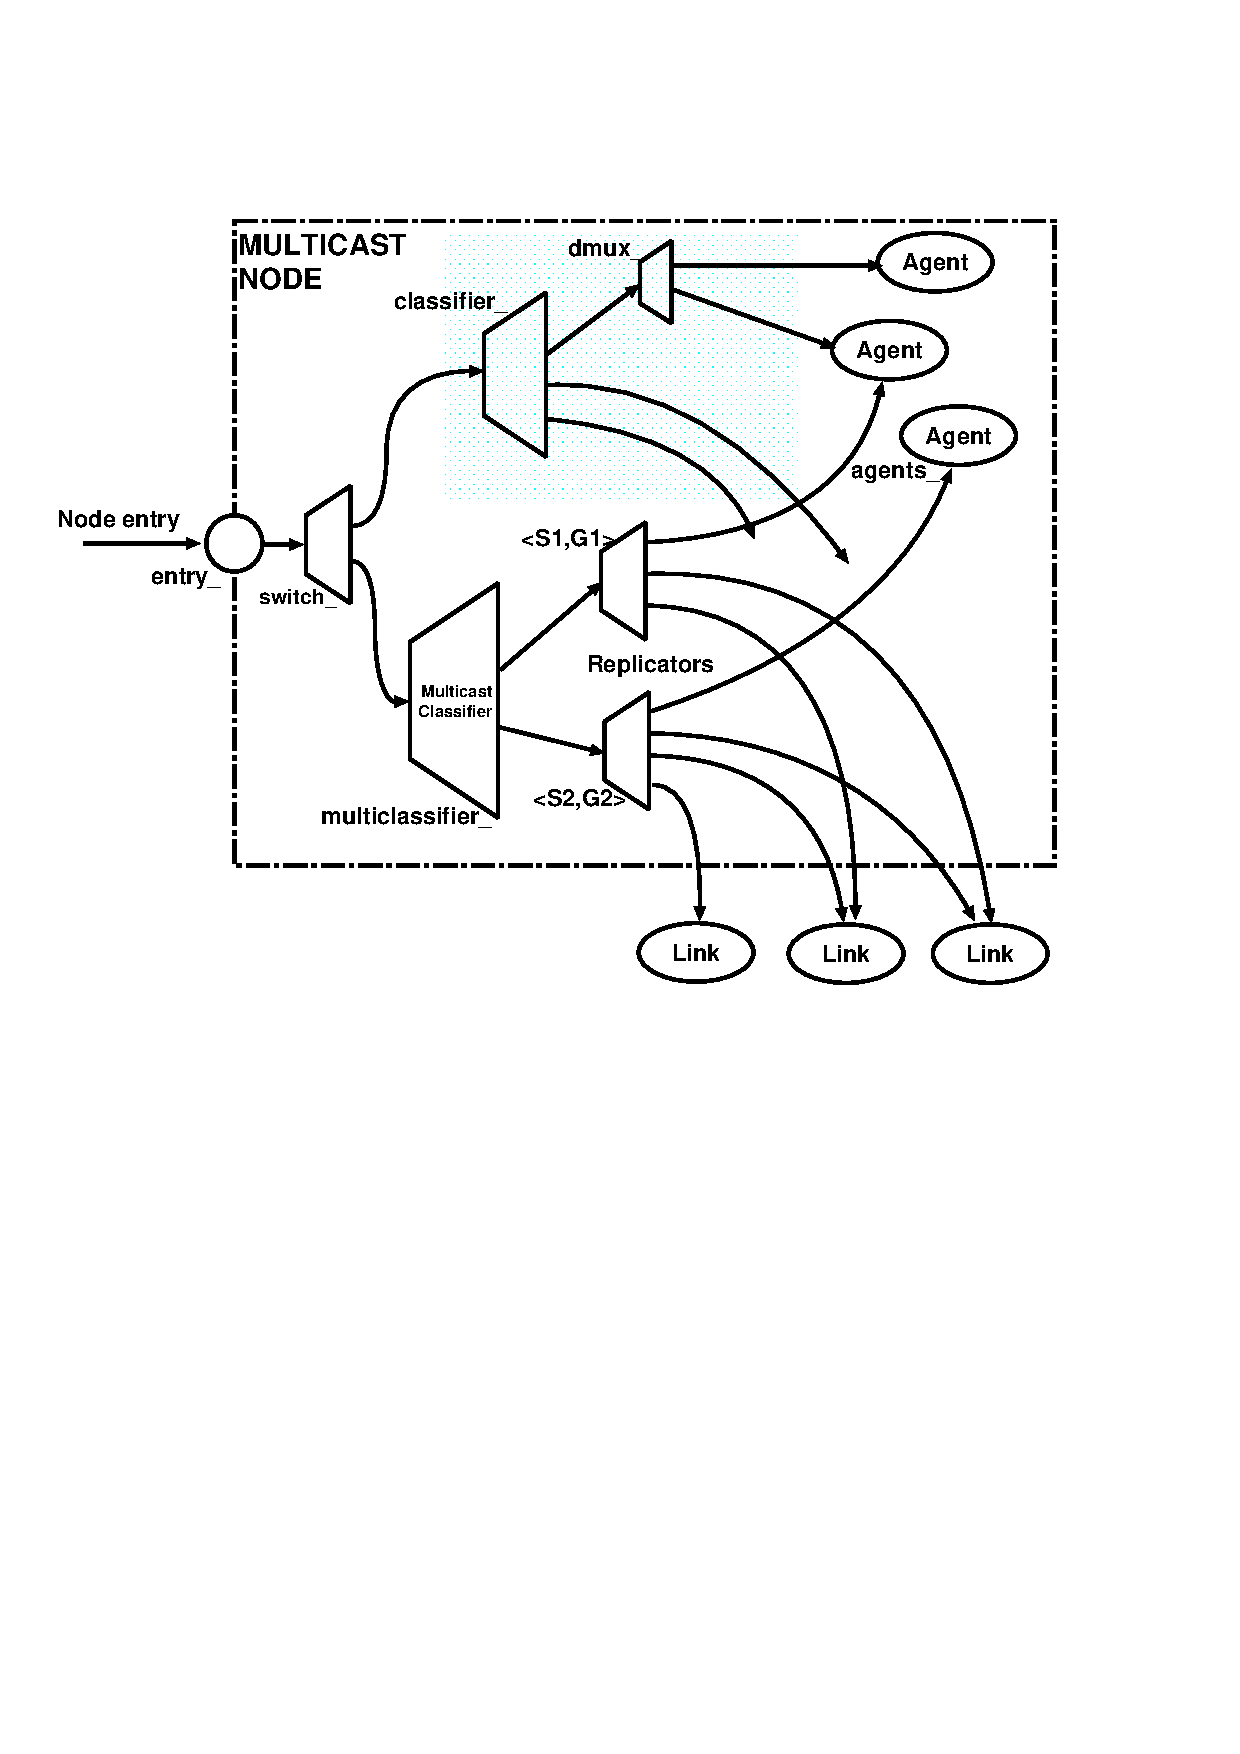
\includegraphics{mcastNode}}
  \caption{Internal Structure of a Multicast Node.}
  \label{fig:node:multicast}
\end{figure}

When a simulation uses multicast routing,
the highest bit of the address indicates whether the particular
address is a multicast address or an unicast address.
If the bit is 0, the address represents a unicast address,
else the address represents a multicast address.
% This implies that, by default, 
% a multicast simulation is restricted to 128 nodes.

\section{Node Methods: Configuring the Node}
\label{sec:node:node}

Procedures to configure an individual node can be classified into:
\begin{list}{---}{\itemsep0pt}
\item Control functions
\item Address and Port number management, unicast routing functions
\item Agent management
\item Adding neighbors
\end{list}
We describe each of the functions in the following paragraphs.

\paragraph{Control functions}
\begin{enumerate}
\item \code{$node entry} %$
returns the entry point for a node.
This is the first element which will handle packets arriving at that node.

The Node instance variable, \code{entry_}, stores the reference this element.
For unicast nodes, this is the address classifier that looks at the higher
bits of the destination address.
The instance variable, \code{classifier_} contains the reference to this
classifier.
However, for multicast nodes, the entry point is the
\code{switch_} which looks at the first bit to decide whether
it should forward the packet to the unicast classifier, or the multicast
classifier as appropriate.

\item \code{$node reset} %$
will reset all agents at the node.
\end{enumerate}


\paragraph{Address and Port number management}
The procedure \code{$node id} %$
returns the node number of the node.
This number is automatically incremented and assigned to each node at
creation by the class Simulator method, \code{$ns node}.%$
The class Simulator also stores an instance variable array\footnote{%
  \ie, an instance variable of a class that is also an array variable},
  \code{Node_}, indexed by the node id, and contains a reference to the
  node with that id.

The procedure \code{$node agent \tup{port}} %$
returns the handle of the
agent at the specified port.
If no agent at the specified port number is available, the procedure returns
the null string.

The procedure \code{alloc-port} returns the next available port number.
It uses an instance variable, \code{np_},
to track the next unallocated port number.

The procedures, \code{add-route} and \code{add-routes},
are used by \href{unicast routing}{Chapter}{chap:unicast}
to add routes to populate the \code{classifier_}
The usage syntax is
\code{$node add-route \tup{destination id} \tup{TclObject}}. %$
\code{TclObject} is the entry of \code{dmux_}, the port demultiplexer
at the node, if the destination id is the same as this node's id,
it is often the head of a link to send packets for that destination to,
but could also be the the entry for other classifiers or types of classifiers.

\code{$node add-routes \tup{destination id} \tup{TclObjects}} %$
is used to add multiple routes to the same destination that must be used
simultaneously in round robin manner to spread the bandwidth used to reach
that destination across all links equally.
It is used only if the instance variable \code{multiPath_} is set to 1,
and detailed dynamic routing strategies are in effect,
and requires the use of a multiPath classifier.
We describe the implementation of the multiPath classifier
\href{later in this chapter}{Section}{sec:node:classifiers};
however, \href{we defer the discussion of multipath
routing}{Chapter}{chap:unicast} to the chapter on unicast routing.

The dual of \proc[]{add-routes} is \proc[]{delete-routes}.
It takes the id, a list of \code{TclObjects}, and a reference to
the simulator's \code{nullagent}.
It removes the TclObjects in the list from the installed routes in the
multipath classifier.
If the route entry in the classifier does not point to a multipath
classifier,
the routine simply clears the entry from \code{classifier_}, and
installs the \code{nullagent} in its place.

Detailed dynamic routing also uses two additional methods:
the instance procedure \proc[]{init-routing} sets the instance variable
\code{multiPath_} to be equal to the class variable of the same name.
It also adds a reference to the route controller object at that node
in the instance variable, \code{rtObject_}.
The procedure \proc[]{rtObject?} returns the handle for the route object 
at the node.

Finally, the procedure \proc[]{intf-changed} is invoked by
the network dynamics code if a link incident on the node
changes state.  Additional details on how this procedure
is used are discussed later
\href{in the chapter on network dynamics}{Chapter}{chap:net-dynamics}.

\paragraph{Agent management}
Given an \tup{agent}, the procedure \proc[]{attach} will
add the agent to its list of \code{agents_},
assign a port number the agent and set its source address,
set the target of the agent to be its (\ie, the node's) \proc[]{entry},
and add a pointer to the port demultiplexer at the node (\code{dmux_})
to the agent at the corresponding slot in the \code{dmux_} classifier.

Conversely, \proc[]{detach}will remove the agent from \code{agents_},
and point the agent's target, and the entry in the node \code{dmux_}
to \code{nullagent}.

\paragraph{Tracking Neighbors}
Each node keeps a list of its adjacent neighbors in its instance variable,
\code{neighbor_}.  The procedure \proc[]{add-neighbor} adds a neighbor to the list.  The procedure \proc[]{neighbors} returns this list.

\section{Node Configuration Interface}
\label{sec:node:nodeconfig}

\framebox{
  \begin{minipage}{\textwidth}
    {\bf NOTE}: This API, especially its internal implementation which
    is messy at this point, is still a moving target. It may undergo
    significant changes in the near future. However, we will do our
    best to maintain the same interface as described in this chapter.
    In addition, this API currently does not cover all existing nodes
    in the old format, namely, nodes built using inheritance, and
    parts of mobile IP. It is principally oriented towards wireless
    and satellite simulation.
    [Sep 15, 2000; updated June 2001].
  \end{minipage}
}

\proc[]{Simulator::node-config} accommodates flexible and modular
construction of different node definitions within the same base Node
class.
For instance, to create a mobile node capable
of wireless communication, one no longer needs a specialized node
creation command, e.g., \proc[]{dsdv-create-mobile-node}; instead, one
changes default configuration parameters, such as  
\begin{program}
$ns node-config -adhocRouting dsdv 
\end{program}
before actually 
creating the node with the command: \code{$ns node}.
Together with routing modules, this allows
one to combine ``arbitrary'' routing functionalities within a single
node without resorting to multiple inheritance and other fancy object
gimmicks. 
We will describe this in more detail in Section~\ref{sec:node:rtarch}.
The functions and procedures relevant to the new node APIs may be
found in \nsf{tcl/lib/ns-node.tcl}.

The node configuration interface consists of two parts. 
The first part deals with node configuration, while the second part
actually creates nodes of the specified type. 
We have already seen the latter in Section~\ref{sec:node:simulator},
in this section we will describe the configuration part. 

Node configuration essentially consists of defining the different node
characteristics before creating them. They may consist of the type of
addressing structure used in the simulation, defining the network
components for mobilenodes, turning on or off the trace options at
Agent/Router/MAC levels, selecting the type of adhoc routing protocol for
wireless nodes or defining their energy model.

As an example, node-configuration for a wireless, mobile node that 
runs AODV as its
adhoc routing protocol in a hierarchical topology would be as shown below.
We decide to turn tracing on at the agent and router level only. Also we 
assume a topology has been instantiated with "set topo [new Topography]". 
The node-config command would look like the following:

\begin{program}
  \$ns_ node-config -addressType hierarchical \bs 
                   -adhocRouting AODV \bs
                   -llType LL \bs
                   -macType Mac/802_11 \bs 
                   -ifqType Queue/DropTail/PriQueue \bs
                   -ifqLen 50 \bs
                   -antType Antenna/OmniAntenna \bs 
                   -propType Propagation/TwoRayGround \bs
                   -phyType Phy/WirelessPhy \bs
                   -topologyInstance \$topo \bs
                   -channel Channel/WirelessChannel \bs 
                   -agentTrace ON \bs 
                   -routerTrace ON \bs
                   -macTrace OFF \bs
                   -movementTrace OFF 
\end{program}

The default values for all the above options are NULL except 
\code{-addressingType}
whose default value is flat. The option \code{-reset} can be used to reset all
node-config parameters to their default value.

Note that the config command can be broken down into separate lines like
\begin{program}
        \$ns_ node-config -addressingType hier
        \$ns_ node-config -macTrace ON
\end{program}
The options that need to be changed may only be called. For example after
configuring for AODV mobilenodes as shown above (and after creating AODV
mobilenodes), we may configure for AODV base-station nodes in the
following way: 
\begin{program}
        \$ns_ node-config -wiredRouting ON
\end{program}
While all other features for base-station nodes and mobilenodes are same,
the base-station nodes are capable of wired routing, while mobilenodes are
not. In this way we can change node-configuration only when it is required.

All node instances created after a given node-configuration command will
have the same property unless a part or all of the node-config command is
executed with different parameter values. And all parameter values remain
unchanged unless they are expicitly changed. So after creation of the AODV
base-station and mobilenodes, if we want to create simple nodes, we will
use the following node-configuration command:
\begin{program}
        \$ns_ node-config -reset
\end{program}
This will set all parameter values to their default setting which
basically defines configuration of a simple node.

Currently, this type of node configuration is oriented towards wireless
and satellite nodes.  Table 5.1
%% ~\ref{table:nodeconfig} 
lists the available options
for these kinds of nodes.  The example scripts 
\nsf{tcl/ex/simple-wireless.tcl} and \nsf{tcl/ex/sat-mixed.tcl} provide
usage examples.

\begin{table}[ht]
\label{table:nodeconfig}
\begin{center} 
{\footnotesize
\begin{tabular}{|l|l|l|}\hline
{\bf option} & {\bf available values} & {\bf default}\\\hline\hline 
\multicolumn{3}{|c|}{\bf general} \\\hline
{\bf addressType} & flat, hierarchical & flat\\\hline
{\bf MPLS} & ON, OFF & OFF\\\hline
\multicolumn{3}{|c|}{\bf both satellite- and wireless-oriented} \\\hline
{\bf wiredRouting} & ON, OFF & OFF\\\hline
{\bf llType} & LL, LL/Sat & "" \\\hline
{\bf macType} & Mac/802\_11, Mac/Csma/Ca, Mac/Sat, & \\ 
& Mac/Sat/UnslottedAloha, Mac/Tdma & "" \\\hline
{\bf ifqType} & Queue/DropTail, Queue/DropTail/PriQueue & "" \\\hline
{\bf phyType} & Phy/WirelessPhy, Phy/Sat& "" \\\hline
\multicolumn{3}{|c|}{\bf wireless-oriented} \\\hline
{\bf adhocRouting} & DIFFUSION/RATE, DIFFUSION/PROB, DSDV, & \\
& DSR, FLOODING, OMNIMCAST, AODV, TORA, M-DART & \\
& PUMA & ""\\\hline
{\bf propType} & Propagation/TwoRayGround, Propagation/Shadowing & ""\\\hline
{\bf propInstance} & Propagation/TwoRayGround, Propagation/Shadowing & ""\\\hline
{\bf antType} & Antenna/OmniAntenna & ""\\\hline
{\bf channel} & Channel/WirelessChannel, Channel/Sat & ""\\\hline
{\bf topoInstance} & <topology file> & ""\\\hline
{\bf mobileIP} & ON, OFF& OFF \\\hline
{\bf energyModel} & EnergyModel & "" \\\hline
{\bf initialEnergy} & <value in Joules> & "" \\\hline
{\bf rxPower} & <value in W> & "" \\\hline
{\bf txPower} & <value in W> & "" \\\hline
{\bf idlePower} & <value in W> & "" \\\hline
{\bf agentTrace} & ON, OFF & OFF \\\hline
{\bf routerTrace} & ON, OFF & OFF \\\hline
{\bf macTrace} & ON, OFF & OFF \\\hline
{\bf movementTrace} & ON, OFF & OFF \\\hline
{\bf errProc} & UniformErrorProc & "" \\\hline
{\bf FECProc} &? & ? \\\hline
{\bf toraDebug} & ON, OFF & OFF \\\hline
\multicolumn{3}{|c|}{\bf satellite-oriented} \\\hline
{\bf satNodeType} & polar, geo, terminal, geo-repeater & "" \\\hline
{\bf downlinkBW} & <bandwidth value, e.g. "2Mb"> & ""\\\hline
\end{tabular}
}
\end{center}
\caption{Available options for node configuration (see tcl/lib/ns-lib.tcl).
}
\end{table}
\normalsize

\section{The Classifier}
\label{sec:node:classifiers}

The function of a node when it receives a packet is to examine
the packet's fields, usually its destination address, and
on occasion, its source address.
It should then map the values to an outgoing interface object
that is the next downstream recipient of this packet.

In \ns, this task is performed by a simple \emph{classifier} object.
Multiple classifier objects,
each looking at a specific portion of the packet
forward the packet through the node.
A node in \ns\ uses many different types of classifiers for different purposes.
This section describes some of the more common, or simpler,
classifier objects in \ns.

We begin with a description of the base class in this section.
The next subsections describe
\href{the address classifier}{Section}{sec:node:addr-classifier},
\href{the multicast classifier}{Section}{sec:node:mcast-classifier},
\href{the multipath classifier}{Section}{sec:node:mpath-classifier}, 
\href{the hash classifier}{Section}{sec:node:hash-classifier}, and
finally, \href{the replicator}{Section}{sec:node:replicator}.

A classifier provides a way to match a packet against some
logical criteria and retrieve a reference to another simulation
object based on the match results.
Each classifier contains a table of simulation objects indexed
by {\em slot number}.
The job of a classifier is to determine the slot number associated
with a received packet and forward that packet to the
object referenced by that particular slot.
The C++ \clsref{Classifier}{../ns-2/classifier.h}
(defined in \nsf{classifier.h})
provides a base class from which other classifiers are derived.
\begin{program}
        class Classifier : public NsObject \{
        public:
                ~Classifier();
                void recv(Packet*, Handler* h = 0);
         protected:
                Classifier();
                void install(int slot, NsObject*);
                void clear(int slot);
                virtual int command(int argc, const char*const* argv);
                virtual int classify(Packet *const) = 0;
                void alloc(int);
                NsObject** slot_;       \* table that maps slot number to a NsObject */
                int nslot_;
                int maxslot_;
        \};
\end{program}
The \fcn[]{classify} method is pure virtual, indicating the
class \code{Classifier} is to be used only as a base class.
The \fcn[]{alloc} method dynamically allocates enough space
in the table to hold the specified number of slots.
The \fcn[]{install} and \fcn[]{clear} methods
add or remove objects from the table.
The \fcn[]{recv} method and the OTcl interface are implemented
as follows in \nsf{classifier.cc}:
\begin{program}
        /*
         *{\cf objects only ever see "packet" events, which come either}
         *{\cf from an incoming link or a local agent (i.e., packet source).}
         */
        void Classifier::recv(Packet* p, Handler*)
        \{
                NsObject* node;
                int cl = classify(p);
                if (cl < 0 || cl >= nslot_ || (node = slot_[cl]) == 0) \{
                        Tcl::instance().evalf("%s no-slot %d", name(), cl);
                        Packet::free(p);
                        return;
                \}
                node->recv(p);
        \}

        int Classifier::command(int argc, const char*const* argv)
        \{
                Tcl& tcl = Tcl::instance();
                if (argc == 3) \{
                        /*
                         * $classifier clear $slot
                         */
                        if (strcmp(argv[1], "clear") == 0) \{
                                int slot = atoi(argv[2]);
                                clear(slot);
                                return (TCL_OK);
                        \}
                        /*
                         * $classifier installNext $node
                         */
                        if (strcmp(argv[1], "installNext") == 0) \{
                                int slot = maxslot_ + 1;
                                NsObject* node = (NsObject*)TclObject::lookup(argv[2]);
                                install(slot, node);
                                tcl.resultf("%u", slot);
                                return TCL_OK;
                        \}
                        if (strcmp(argv[1], "slot") == 0) \{
                                int slot = atoi(argv[2]);
                                if ((slot >= 0) || (slot < nslot_)) \{
                                        tcl.resultf("%s", slot_[slot]->name());
                                        return TCL_OK;
                                \}
                                tcl.resultf("Classifier: no object at slot %d", slot);
                                return (TCL_ERROR);
                        \}
                \} else if (argc == 4) \{
                        /*
                         * $classifier install $slot $node
                         */
                        if (strcmp(argv[1], "install") == 0) \{
                                int slot = atoi(argv[2]);
                                NsObject* node = (NsObject*)TclObject::lookup(argv[3]);
                                install(slot, node);
                                return (TCL_OK);
                        \}
                \}
                return (NsObject::command(argc, argv));
        \}
\end{program} %$
When a classifier \fcn[]{recv}'s a packet,
it hands it to the \fcn[]{classify} method.
This is defined differently in each type of classifier
derived from the base class.
The usual format is for the \fcn[]{classify} method to
determine and return a slot index into the table of slots.
If the index is valid, and points to a valid TclObject,
the classifier will hand the packet to that object using 
that object's \fcn[]{recv} method.
If the index is not valid, the classifier will invoke
the instance procedure \proc[]{no-slot} to attempt to 
populate the table correctly.
However, in the base class \proc[]{Classifier::no-slot} prints
and error message and terminates execution.

The \fcnref{\fcn[]{command} method}{../ns-2/classifier.cc}{Classifier::command}
provides the following instproc-likes to the interpreter:
\begin{itemize}\itemsep0pt
\item \proc[\tup{slot}]{clear} clears the entry in a particular slot.
\item \proc[\tup{object}]{installNext} installs the object
        in the next available slot, and returns the slot number.

        Note that this instproc-like is 
        \fcnref{overloaded by an instance procedure of the same name}{%
                ../ns-2/ns-lib.tcl}{Classifier::installNext}
        that stores a reference to the object stored.
        This then helps quick query of the objects
        installed in the classifier from OTcl.
\item \proc[\tup{index}]{slot} returns the object stored in the specified slot.
\item \proc[\tup{index}, \tup{object}]{install} installs the specified
        \tup{object} at the slot \tup{index}.

        Note that this instproc-like too is 
        \fcnref{overloaded by an instance procedure of the same name}{%
                ../ns-2/ns-lib.tcl}{Classifier::install}
        that stores a reference to the object stored.
        This is also to quickly query of the objects
        installed in the classifier from OTcl.
\end{itemize}

\subsection{Address Classifiers}
\label{sec:node:addr-classifier}

An address classifier is used in supporting unicast packet forwarding.
It applies a bitwise shift and mask operation to a packet's destination
address to produce a slot number.
The slot number is returned from the \fcn[]{classify} method.
The \clsref{AddressClassifier}{../ns-2/classifier-addr.cc}
(defined in \nsf{classifier-addr.cc}) ide defined as follows:
\begin{program}
        class AddressClassifier : public Classifier \{
        public:
                AddressClassifier() : mask_(~0), shift_(0) \{
                        bind("mask_", (int*)&mask_);
                        bind("shift_", &shift_);
                \}
        protected:
                int classify(Packet *const p) \{
                        IPHeader *h = IPHeader::access(p->bits());
                        return ((h->dst() >> shift_) & mask_);
                \}
                nsaddr_t mask_;
                int shift_;
        \};
\end{program}
The class imposes no direct semantic meaning
on a packet's destination address field.
Rather, it returns some number of bits from the packet's
\code{dst_} field as the slot number used
in the \fcnref{\fcn[]{Classifier::recv}}{../ns-2/classifier.cc}{Classifier::recv} method.
The \code{mask_} and \code{shift_} values are set through OTcl.

\subsection{Multicast Classifiers}
\label{sec:node:mcast-classifier}

The multicast classifier classifies packets
according to both source and destination (group) addresses.
It maintains a (chained hash) table mapping source/group pairs to slot numbers.
When a packet arrives containing a source/group unknown to the classifier,
it invokes an Otcl procedure \proc[]{Node::new-group}
to add an entry to its table.
This OTcl procedure may use the method \code{set-hash} to add
new (source, group, slot) 3-tuples to the classifier's table.
The multicast classifier is defined in \nsf{classifier-mcast.cc}
as follows:
\begin{program}
        static class MCastClassifierClass : public TclClass \{
        public:
                MCastClassifierClass() : TclClass("Classifier/Multicast") \{\}
                TclObject* create(int argc, const char*const* argv) \{
                        return (new MCastClassifier());
                \}
        \} class_mcast_classifier;

        class MCastClassifier : public Classifier \{
        public:
                MCastClassifier();
                ~MCastClassifier();
        protected:
                int command(int argc, const char*const* argv);
                int classify(Packet *const p);
                int findslot();
                void set_hash(nsaddr_t src, nsaddr_t dst, int slot);
                int hash(nsaddr_t src, nsaddr_t dst) const \{
                        u_int32_t s = src ^ dst;
                        s ^= s >> 16;
                        s ^= s >> 8;
                        return (s & 0xff);
                \}
                struct hashnode \{
                        int slot;
                        nsaddr_t src;
                        nsaddr_t dst;
                        hashnode* next;
                \};
                hashnode* ht_[256];
                const hashnode* lookup(nsaddr_t src, nsaddr_t dst) const;
        \};

        int MCastClassifier::classify(Packet *const pkt)
        \{
                IPHeader *h = IPHeader::access(pkt->bits());
                nsaddr_t src = h->src() >> 8; /*XXX*/
                nsaddr_t dst = h->dst();
                const hashnode* p = lookup(src, dst);
                if (p == 0) \{
                        /*
                         * Didn't find an entry.
                         * Call tcl exactly once to install one.
                         * If tcl doesn't come through then fail.
                         */
                        Tcl::instance().evalf("%s new-group %u %u", name(), src, dst);
                        p = lookup(src, dst);
                        if (p == 0)
                                return (-1);
                \}
                return (p->slot);
        \}
\end{program}
The \clsref{MCastClassifier}  implements a chained hash table
and applies a hash function on both the packet source and
destination addresses.
The hash function returns the slot number
to index the \code{slot_} table in the underlying object.
A hash miss implies packet delivery to a previously-unknown group;
OTcl is called to handle the situation.
The OTcl code is expected to insert an appropriate entry into the hash table.

\subsection{MultiPath Classifier}
\label{sec:node:mpath-classifier}

This object is devised to support equal cost multipath
forwarding, where the node has multiple equal cost routes
to the same destination, and would like to use all of them
simultaneously.
This object does not look at any field in the packet.
With every succeeding packet, 
it simply returns the next filled slot in round robin fashion.
The definitions for this classifier are in \nsf{classifier-mpath.cc},
and are shown below:
\begin{program}
class MultiPathForwarder : public Classifier \{
public:
        MultiPathForwarder() : ns_(0), Classifier() \{\} 
        virtual int classify(Packet* const) \{
                int cl;
                int fail = ns_;
                do \{
                        cl = ns_++;
                        ns_ %= (maxslot_ + 1);
                \} while (slot_[cl] == 0 && ns_ != fail);
                return cl;
        \}
private:
        int ns_;     \* next slot to be used.  Probably a misnomer? */
\};
\end{program}

\subsection{Hash Classifier}
\label{sec:node:hash-classifier}

This object is used to classify a packet as a member of a
particular {\em flow}.
As their name indicates,
hash classifiers use a hash table internally to assign
packets to flows.
These objects are used where flow-level information is
required (e.g. in flow-specific queuing disciplines and statistics
collection).
Several ``flow granularities'' are available.  In particular,
packets may be assigned to flows based on flow ID, destination address,
source/destination addresses, or the combination of source/destination
addresses plus flow ID.
The fields accessed by the hash classifier are limited to
the {\tt ip} header: {\tt src(), dst(), flowid()} (see {\tt ip.h}).

The hash classifier is created with an integer argument specifying
the initial size of its hash table.  The current hash table size may
be subsequently altered with the {\tt resize} method (see below).
When created, the instance variables \code{shift_} and \code{mask_}
are initialized with the simulator's current {\sf NodeShift} and
{\sf NodeMask} values, respectively.  These values are retrieved
from the {\tt AddrParams} object when the hash classifier is
instantiated.  The hash classifier will fail to operate properly if
the {\tt AddrParams} structure is not initialized.
The following constructors are used for the various hash classifiers:
\begin{program}
        Classifier/Hash/SrcDest
        Classifier/Hash/Dest
        Classifier/Hash/Fid
        Classifier/Hash/SrcDestFid
\end{program}

The hash classifier receives packets, classifies them according
to their flow criteria, and retrieves the classifier {\em slot}
indicating the next node that should receive the packet.
In several circumstances with hash classifiers, most packets should
be associated with a single slot, while only a few flows should
be directed elsewhere. 
The hash classifier includes a \code{default_} instance variable
indicating which slot is to be used for packets that do not match
any of the per-flow criteria.
The \code{default_} may be set optionally.

The methods for a hash classifier are as follows:
\begin{program}
        $hashcl set-hash buck src dst fid slot
        $hashcl lookup buck src dst fid
        $hashcl del-hash src dst fid
        $hashcl resize nbuck
\end{program}

The \fcn[]{set-hash} method inserts a new entry into the hash
table within the hash classifier.
The {\tt buck} argument specifies the hash table bucket number
to use for the insertion of this entry.
When the bucket number is not known, {\tt buck} may be specified
as {\tt auto}. 
The {\tt src, dst} and {\tt fid} arguments specify the IP source,
destination, and flow IDs to be matched for flow classification.
Fields not used by a particular classifier (e.g. specifying {\tt src}
for a flow-id classifier) is ignored.
The {\tt slot} argument indicates the index into the underlying
slot table in the base {\tt Classifier} object from which
the hash classifier is derived.
The {\tt lookup} function returns the name of the object
associated with the given {\tt buck/src/dst/fid} tuple.
The {\tt buck} argument may be {\tt auto}, as for {\tt set-hash}.
The {\tt del-hash} function removes the specified entry from
the hash table.
Currently, this is done by simply marking the entry as inactive,
so it is possible to populate the hash table with unused entries.
The {\tt resize} function resizes the hash table to include
the number of buckets specified by the argument {\tt nbuck}.

Provided no default is defined, a hash classifier will
perform a call into OTcl when it
receives a packet which matches no flow criteria.
The call takes the following form:
\begin{program}
        \$obj unknown-flow src dst flowid buck
\end{program} 
Thus, when a packet matching no flow criteria is received,
the method {\tt unknown-flow} of the instantiated hash classifier
object is invoked with the source, destination, and flow id
fields from the packet.
In addition, the {\tt buck} field indicates the hash bucket
which should contain this flow if it were inserted using
{\tt set-hash}.  This arrangement avoids another hash
lookup when performing insertions into the classifier when the
bucket is already known.

\subsection{Replicator}
\label{sec:node:replicator}

The replicator is different from the other classifiers
we have described earlier,
in that it does not use the classify function.
Rather, it simply uses the classifier as a table of $n$ slots;
it overloads the \fcn[]{recv} method to produce $n$ copies
of a packet, that are delivered to all $n$ objects referenced in the table.

To support multicast packet forwarding, a classifier receiving a
multicast packet from source $S$
destined for group $G$ computes a hash function $h(S,G)$ giving
a ``slot number'' in the classifier's object table.
%Thus, the maximum size of the table is $O(|S|\times|G|)$.
In multicast delivery, the packet must be copied once for
each link leading to nodes subscribed to $G$ minus one.
Production of additional copies of the packet is performed
by a \code{Replicator} class, defined in \code{replicator.cc}:
\begin{program}
        /*
         * {\cf A replicator is not really a packet classifier but}
         * {\cf we simply find convenience in leveraging its slot table.}
         * {\cf (this object used to implement fan-out on a multicast}
         * {\cf router as well as broadcast LANs)}
         */
        class Replicator : public Classifier \{
        public:
                Replicator();
                void recv(Packet*, Handler* h = 0);
                virtual int classify(Packet* const) \{\};
        protected:
                int ignore_;
        \};

        void Replicator::recv(Packet* p, Handler*)
        \{
                IPHeader *iph = IPHeader::access(p->bits());
                if (maxslot_ < 0) \{
                        if (!ignore_)
                                Tcl::instance().evalf("%s drop %u %u", name(), 
                                        iph->src(), iph->dst());
                        Packet::free(p);
                        return;
                \}
                for (int i = 0; i < maxslot_; ++i) \{
                        NsObject* o = slot_[i];
                        if (o != 0)
                                o->recv(p->copy());
                \}
                /* {\cf we know that maxslot is non-null} */
                slot_[maxslot_]->recv(p);
        \}
\end{program}
As we can see from the code,
this class  does not really classify packets.
Rather, it replicates a packet, one for each entry in its table,
and delivers the copies to each of the nodes listed in the table.
The last entry in the table gets the ``original'' packet.
Since the \fcn[]{classify} method is pure virtual in the base class,
the replicator defines an empty \fcn[]{classify} method.

\section{Routing Module and Classifier Organization}
\label{sec:node:rtarch}

As we have seen, a \ns\ node is essentially a collection of
classifiers.
The simplest node (unicast) contains only one address classifier and
one port classifier, as shown in Figure~\ref{fig:node:unicast}.
When one extends the functionality of the node, more classifiers are added
into the base node, for instance, the multicast node shown in
Figure~\ref{fig:node:multicast}.
As more function blocks is added, and each of these blocks requires
its own classifier(s), it becomes important for the node to
provide a {\em uniform} interface to organize these classifiers and to
bridge these classifiers to the route computation blocks.

The classical method to handle this case is through class
inheritance.
For instance, if one wants a node that supports hierarchical routing,
one simply derive a Node/Hier from the base node and override the
classifier setup methods to insert hierarchical classifiers.
This method works well when the new function blocks are independent
and cannot be ``arbitrarily'' mixed. 
For instance, both hierarchical routing and ad hoc routing use their
own set of classifiers. 
Inheritance would require that we have Node/Hier that supports
the former, and Node/Mobile for the latter.
This becomes slightly problematic when one wants an ad hoc routing
node that supports hierarchical routing.
In this simple case one may use multiple inheritance to solve the
problem, but this quickly becomes infeasible as the number of such
function blocks increases. 

The only method to solve this problem is object composition. 
The base node needs to define a set of interfaces for classifier
access and organization. 
These interfaces should
\begin{itemize}
\item allow individual routing modules that implement
  their own classifiers to insert their classifiers into the node;
\item allow route computation blocks to populate routes to classifiers
  in all routing modules that need this information, 
\item provide a single point of management for existing routing modules. 
\end{itemize}
In addition, we should also define a uniform interface for routing
modules to connect to the node interfaces, so as to provide a
systematic approach to extending node functionality. 
In this section we will describe the design of routing modules as well
as that of the corresponding node interfaces.

\subsection{Routing Module}

In general, every routing implementation in \ns\ consists of three
function blocks: 
\begin{itemize}
\item {\em Routing agent} exchanges routing packet with neighbors, 
\item {\em Route logic} uses the information gathered by routing
  agents (or the global topology database in the case of static
  routing) to perform the actual route computation, 
\item {\em Classifiers} sit inside a Node. They use the computed
  routing table to perform packet forwarding.
\end{itemize}
Notice that when implementing a new routing protocol, one does not
necessarily implement all of these three blocks.
For instance, when one implements a link state routing protocol, one
simply implement a routing agent that exchanges information in the
link state manner, and a route logic that does Dijkstra on the
resulting topology database. 
It can then use the same classifiers as other unicast routing
protocols.

\begin{figure}[tb]
  \begin{center}
    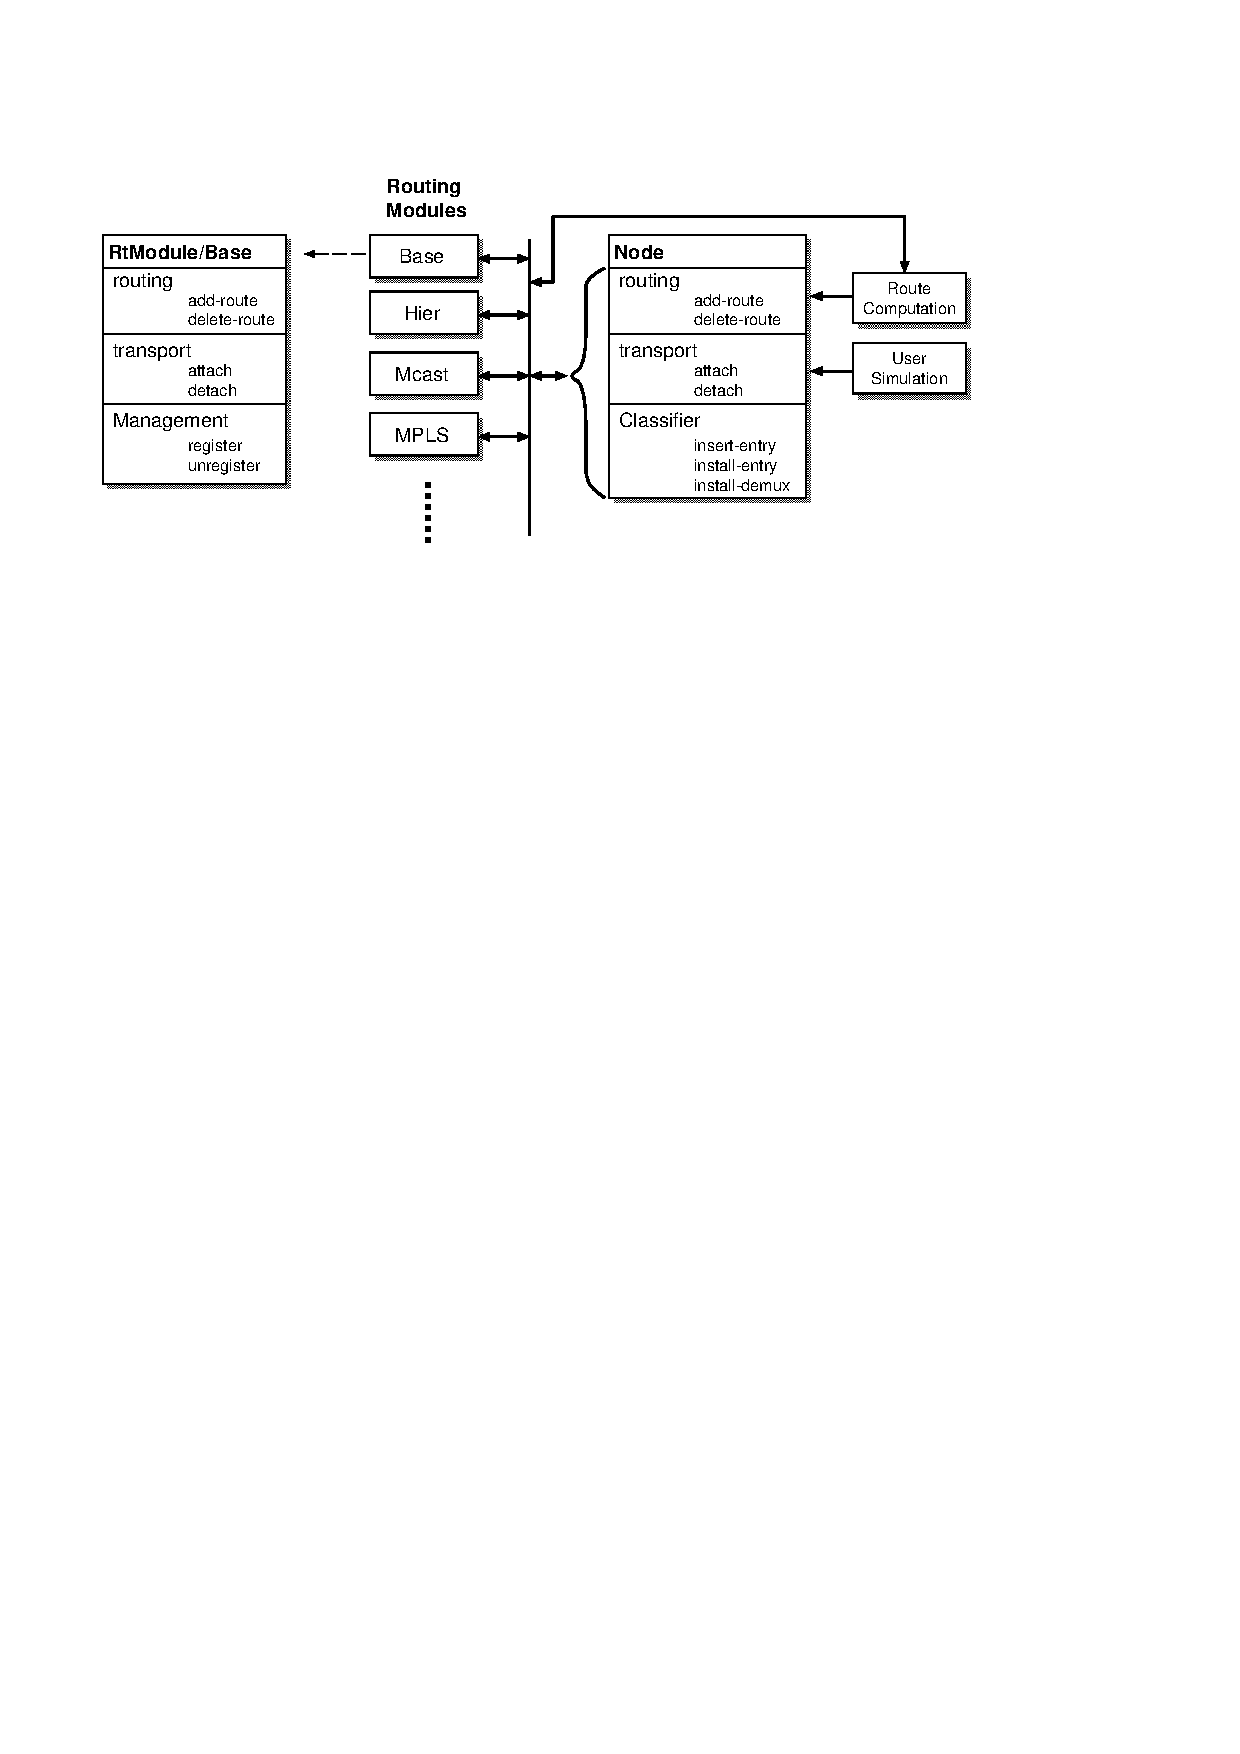
\includegraphics{rtmodule}
    \caption{Interaction among node, routing module, and routing. The
      dashed line shows the details of one routing module.}
    \label{fig:node:rtmodule}
  \end{center}
\end{figure}

When a new routing protocol implementation includes more than one
function blocks, especially when it contains its own classifier, it is
desirable to have another object, which we call 
a {\em routing module}, that manages all these function 
blocks and to interface with node to organize its classifiers.
Figure~\ref{fig:node:rtmodule} shows functional relation among these
objects.
Notice that routing modules may have direct relationship with route
computation blocks, i.e., route logic and/or routing agents.
However, route computation MAY not install their routes directly
through a routing module, because there may exists other modules that
are interested in learning about the new routes.
This is not a requirement, however, because it is possible that some
route computation is specific to one particular routing module, for
instance, label installation in the MPLS module. 

A routing module contains three major functionalities:
\begin{enumerate}
\item %Management
  A routing module initializes its connection to a node through
  \proc[]{register}, and tears the connection down via
  \proc[]{unregister}.
  Usually, in \proc[]{register} a routing module (1) tells the node
  whether it
  interests in knowing route updates and transport agent attachments,
  and (2) creates its classifiers and install them in the node
  (details described in the next subsection).
  In \proc[]{unregister} a routing module does the exact opposite: it
  deletes its classifiers and removes its hooks on routing update in
  the node.
\item %Route handler
  If a routing module is interested in knowing routing updates, the
  node will inform the module via \\
  \proc[dst, target]{RtModule::add-route} and
  \proc[dst, nullagent]{RtModule::delete-route}.
\item %Transport agent handler
  If a routing module is interested in learning about transport agent
  attachment and detachment in a node, the node will inform the module
  via \\ 
  \proc[agent, port]{RtModule::attach} and
  \proc[agent, nullagent]{RtModule::detach}.
\end{enumerate}

There are two steps to write your own routing module:
\begin{enumerate}
\item You need to declare the C++ part of your routing
  module (see \nsf{rtmodule.\{cc,h\}}). For many modules this only
  means to declare a virtual method \code{name()} which returns a
  string descriptor of the module. However, you are free to implement
  as much functionality as you like in C++; if necessary you may
  later move functionality from OTcl into C++ for better performance. 
\item You need to look at the above interfaces implemented in the base
  routing module (see \nsf{tcl/lib/ns-rtmodule.tcl}) and decide which
  one you'll inherit, which one you'll override, and put them in OTcl
  interfaces of your own module. 
\end{enumerate}
There are several derived routing module examples in
\nsf{tcl/lib/ns-rtmodule.tcl}, which may serve as templates for your
modules.

Currently, there are six routing modules implemented in \ns:
\begin{table}[htbp]
  \begin{center}
    \begin{tabular}[htbp]{|c|p{5in}|}
      \hline
      Module Name & Functionality \\ 
      \hline \hline
      RtModule/Base & Interface to unicast routing protocols. Provide
        basic functionality to add/delete route and attach/detach
        agents. \\ \hline
      RtModule/Mcast & Interface to multicast routing protocols. Its
        only purpose is establishes multicast classifiers. All other
        multicast functionalities are implemented as instprocs of
        Node. This should be converted in the future. \\ \hline
      RtModule/Hier & Hierarchical routing. It's a wrapper for
        managing hierarchical classifiers and route installation. Can
        be combined with other routing protocols, e.g., ad hoc
        routing. \\ \hline
      RtModule/Manual & Manual routing. \\ \hline
      RtModule/VC & Uses virtual classifier instead of vanilla
        classifier. \\ \hline
      RtModule/MPLS & Implements MPLS functionality. This is the only
        existing module that is completely self-contained and does not
        pollute the Node namespace. \\
      \hline
    \end{tabular}
    \caption{Available routing modules}
    \label{tab:node:rtmodule}
  \end{center}
\end{table}

\subsection{Node Interface}

To connect to the above interfaces of routing module, a node provides
a similar set of interfaces:
\begin{itemize}
\item %Management
  In order to know which module to register during creation, the Node
  class keeps a list of modules as a class variable. 
  The default value of this list contains only the base routing
  module.
  The Node class provides the following two {\em procs} to manipulate
  this module list:
  \begin{alist}
    \proc[name]{Node::enable-module} & If module
    \code{RtModule/[name]} exists, this proc puts [name] into the
    module list. \\ 
    \proc[name]{Node::disable-module} & If
    [name] is in the module 
    list, remove it from the list. 
  \end{alist}
  When a node is created, it goes through the module list of the Node
  class, creates all modules included in the list, and register these
  modules at the node.

  After a node is created, one may use the following instprocs to list
  modules registered at the node, or to get a handle of a module with
  a particular name:
  \begin{alist}
    \proc[]{Node::list-modules} & Return a list of the handles (shadow
    objects) of all registered modules. \\
    \proc[name]{Node::get-module} & Return a
    handle of the 
    registered module whose name matches the given one. Notice that
    any routing module can only have a single instance registered at
    any node.
  \end{alist}
\item %route and port
  To allow routing modules register their interests of routing
  updates, a node object provide the following instprocs:
  \begin{alist}
    \proc[module]{Node::route-notify} & Add \code{module} into route
    update notification list. \\
    \proc[module]{Node::unreg-route-notify} & Remove \code{module}
    from route update notification list. \\
  \end{alist}
  Similarly, the following instprocs provide hooks on the attachment
  of transport agents:
  \begin{alist}
    \proc[module]{Node::port-notify} & Add \code{module} into agent
    attachment notification list. \\
    \proc[module]{Node::unreg-port-notify} & Remove \code{module} from
    agent attachment notification list. \\
  \end{alist}
  Notice that in all of these instprocs, parameter \code{module}
  should be a module handle instead of a module name. 
\item %classifier
  Node provides the following instprocs to manipulate its address and
  port classifiers:
  \begin{itemize}
  \item \proc[module, clsfr, hook]{Node::insert-entry} inserts
    classifier \code{clsfr} into the entry point of the node. It also
    associates the new classifier with \code{module} so that if this
    classifier is removed later, \code{module} will be unregistered.
    If \code{hook} is specified as a number, the existing classifier
    will be inserted into slot \code{hook} of the new classifier. 
    In this way, one may establish a ``chain'' of classifiers; see
    Figure~\ref{fig:node:multicast} for an example.
    {\bf NOTE}: \code{clsfr} needs NOT to be a classifier. In some
    cases one may want to put an agent, or any class derived from
    Connector, at the entry point of a node. In such cases, one simply
    supplies \code{target} to parameter \code{hook}.
  \item \proc[module, clsfr, hook]{Node::install-entry} differs from
    \code{Node::insert-entry} in that it deletes the existing
    classifier at the node entry point, unregisters any associated
    routing module, and installs the new classifier at that point. 
    If \code{hook} is given, and the old classifier is connected into
    a classifier chain, it will connect the chain into slot
    \code{hook} of the new classifier. 
    As above, if \code{hook} equals to \code{target}, \code{clsfr}
    will be treated as an object derived from Connector instead of a
    classifier. 
  \item \proc[demux, port]{Node::install-demux} places the given
    classifier \code{demux} as the default demultiplexer. If
    \code{port} is given, it plugs the existing demultiplexer into
    slot \code{port} of the new one. Notice that in either case it does
    not delete the existing demultiplexer.
  \end{itemize}
\end{itemize}

\section{Commands at a glance}
\label{sec:nodescommand}
\begin{flushleft}

Following is a list of common node commands used in simulation scripts:

\code{$ns_ node [<hier_addr>]}\\ %$
Command to create and return a node instance. If <hier\_addr> is given,
assign the node address to be <hier\_addr>. Note that the latter MUST
only be used when hierarchical addressing is enabled via either
\proc[]{set-address-format hierarchical} or 
\proc[]{node-config -addressType hierarchical}. 

\code{$ns_ node-config -<config-parameter> <optional-val>}\\%$
This command is used to configure nodes. The different config-parameters
are addressingType, different type of the network stack components,
whether tracing will be turned on or not, mobileIP flag is truned or not,
energy model is being used or not etc. An option -reset maybe used to set
the node configuration to its default state. The default setting of 
node-config, i.e if no values are specified, creates a simple node (base
class Node) with flat addressing/routing. For the syntax details see
Section~\ref{sec:node:nodeconfig}.

\code{$node id}\\%$
Returns the id number of the node.

\code{$node node-addr}\\%$
Returns the address of the node. In case of flat addressing, the node address
is same as its node-id. In case of hierarchical addressing, the node address
in the form of a string (viz. "1.4.3") is returned.

\code{$node reset} \\%$
Resets all agent attached to this node.

\code{$node agent <port_num>} \\%$
Returns the handle of the agent at the specified port. If no agent is found
at the given port, a null string is returned.

\code{$node entry}\\%$
Returns the entry point for the node. This is first object that
handles packet receiving at this node.

\code{$node attach <agent> <optional:port_num>}\\%$
Attaches the <agent> to this node. Incase no specific port number is passed,
the node allocates a port number and binds the agent to this port. Thus once
the agent is attached, it receives packets destined for this host
(node) and port. 

\code{$node detach <agent> <null_agent>}\\%$
This is the dual of "attach" described above. It detaches the agent
from this node 
and installs a null-agent to the port this agent was attached. This is
done to handle transit packets that may be destined to the detached
agent. These on-the-fly packets are then sinked  at the null-agent.

\code{$node neighbors}\\%$
This returns the list of neighbors for the node.

\code{$node add-neighbor <neighbor_node>}\\%$
This is a command to add \code{<neighbor_node>} to the list of neighbors 
maintained by the node.

\rule{\linewidth}{0.3mm}
Following is a list of internal node methods:

\code{$node add-route <destination_id> <target>}\\%$
This is used in unicast routing to populate the classifier. The target is a
Tcl object, which may be the entry of \code{dmux_} (port demultiplexer in
the node) incase the \code{<destination_id>} is same as this node-id.
Otherwise it is usually the head of the link for that destination. It
could also be the entry for other classifiers.

\code{$node alloc-port <null_agent>}\\%$
This returns the next available port number.

\code{$node incr-rtgtable-size}\\%$
The instance variable \code{rtsize_} is used to keep track of size of
routing-table in each node. This command is used to increase the
routing-table size every time an routing-entry is added to the
classifiers.

There are other node commands that supports hierarchical
routing, detailed dynamic routing, equal cost multipath
routing, manual routing, and energy model for mobile nodes. These
and other methods described earlier can be found in 
\nsf{tcl/lib/ns-node.tcl} and \nsf{tcl/lib/ns-mobilenode.tcl}.

\end{flushleft}
\endinput
% LocalWords:  ns tcl lib rtmodule addr cc mcast mpath replicator unicast pt ht
% LocalWords:  multicast mcastNode TclObject dmux installNext strcmp argv int
% LocalWords:  atoi NsObject NsObject argc recv instproc OTcl AddressClassifier
% LocalWords:  const IPHeader IPHeader dst nsaddr Otcl MCastClassifierClass src
% LocalWords:  TclClass MCastClassifier findslot struct hashnode pkt XXX evalf
% LocalWords:  MultiPath multipath MultiPathForwarder cl ip flowid ip NodeShift
% LocalWords:  NodeMask AddrParams SrcDest Dest SrcDestFid hashcl nbuck IDs del
% LocalWords:  flor bj LANs iph maxslot Hier onsists tb MPLS RtModule nullagent
% LocalWords:  config config val num alloc incr rtgtable

\chapter{Links: Simple Links}
\label{chap:links}

This is the second aspect of defining the topology.
In \href{the previous chapter}{Chapter}{chap:nodes},
we had described how to create the nodes in the topology in \ns.
We now describe how to create the links to connect the nodes and complete
the topology.
In this chapter, we restrict ourselves to describing the simple
point to point links.
\ns\ supports a variety of other media, including
an emulation of a multi-access LAN using a mesh of simple links,
and other true simulation of wireless and broadcast media.
They will be described in a separate chapter.
The CBQlink is derived from simple links and is a considerably more
complex form of link that is also not described in this chapter.

We begin by describing the commands to create a link in this section.
As with the node being composed of classifiers, 
a simple link is built up from a sequence of connectors.
We also briefly describe some of the connectors in a simple link.
We then describe
\href{the instance procedures that operate on the various components of
defined by some of these connectors}{Section}{sec:links:components}.
We conclude the chapter
\href{with a description the connector object}{Section}{sec:links:connectors},
including brief
descriptions of the common link connectors.

The \clsref{Link}{../ns-2/ns-link.tcl}
is a standalone class in OTcl,
that provides a few simple primitives.
The \clsref{SimpleLink}{../ns-2/ns-link.tcl}
provides the ability to connect two nodes with a point to point link.
\ns\ provides the instance procedure
\fcnref{\proc[]{simplex-link}}{../ns-2/ns-link.tcl}{Simulator::simplex-link}
to form a unidirectional link from one node to another.
The link is in the class SimpleLink.
The following describes the syntax of the simplex link:
\begin{program}
    set ns [new Simulator]
    $ns simplex-link \tup{node0} \tup{node1} \tup{bandwidth} \tup{delay} \tup{queue_type}
\end{program}
The command creates a link from \code{\tup{node0}} to \code{\tup{node1}},
with specified \code{\tup{bandwidth}} and \code{\tup{delay}} characteristics.
The link uses a queue of type \code{\tup{queue_type}}.
The procedure also adds a TTL checker to the link.
Five instance variables define the link:

\centerline{\begin{tabular}{rp{4in}}
	\code{head\_} &	Entry point to the link, it points
			to the first object in the link. \\
	\code{queue\_} & Reference to the main queue element of the link.
			Simple links usually have one queue per link.
			Other more complex types of links may have multiple
			queue elements in the link. \\
	\code{link\_} &	A reference to the element
			that actually models the link,
			in terms of the delay and bandwidth characteristics
			of the link. \\
	\code{ttl\_} &	Reference to the element that manipulates the
			ttl in every packet. \\
	\code{drophead\_} & Reference to an object that is the head of a
			queue of elements that process link drops. \\
	    \end{tabular}}

In addition, if the simulator instance variable, 
\code{$traceAllFile_}, is defined, 
the procedure will add trace elements that track when a packet is
enqueued and dequeued from \code{queue_}.
Furthermore, tracing interposes a drop trace element after the
\code{drophead_}.
\begin{figure}[tb]
  \centerline{\includegraphics{link}}
  \caption{Composite Construction of a Unidirectional Link}
  \label{fig:link}
\end{figure}
The following instance variables track the trace elements:

\centerline{\begin{tabular}{rp{4in}}
	\code{enqT\_} &	Reference to the element that traces
			packets entering \code{queue\_}.\\
	\code{deqT\_} &	Reference to the element that traces
			packets leaving \code{queue\_}.\\
	\code{drpT\_} &	Reference to the element that traces
			packets dropped from \code{queue\_}.\\
	\code{rcvT\_} &	Reference to the element that traces
			packets received by the next node.\\
	    \end{tabular}}

Note however, that if the user enable tracing multiple times on the link,
these instance variables will only store a reference to the
last elements inserted.

Other configuration mechanisms that add components to a simple link
are network interfaces (used in multicast routing), 
link dynamics models, and tracing and monitors.
We give 
\href{a brief overview of the related objects at the end of this chapter}{%
		Section}{sec:links:connectors},
and discuss their functionality/implementation in other chapters.

The instance procedure
\fcnref{\proc[]{duplex-link}}{../ns-2/ns-link.tcl}{Simulator::duplex-link}
constructs a bi-directional link from two simplex links.

\section{Instance Procedures for Links and SimpleLinks}
\label{sec:links:components}

\paragraph{Link procedures}
The \clsref{Link}{../ns-2/ns-link.tcl} is implemented entirely in Otcl.
The OTcl \code{SimpleLink} class uses the C++ \code{LinkDelay} class
to simulate packet delivery delays.
The instance procedures in the class Link are:

\begin{tabularx}{\linewidth}{rX}
\fcnref{\proc[]{head}}{../ns-2/ns-link.tcl}{Link::head} &
		returns the handle for \code{head\_}. \\
\fcnref{\proc[]{queue}}{../ns-2/ns-link.tcl}{Link::queue} &
		returns the handle for \code{queue\_}. \\
\fcnref{\proc[]{link}}{../ns-2/ns-link.tcl}{Link::link} &
		returns the handle for the delay element, \code{link\_}. \\
\fcnref{\proc[]{up}}{../ns-2/ns-link.tcl}{Link::up} &
		set link status to ``up'' in the \code{dynamics\_} element.
		Also, writes out a trace line to each file specified through
		the procedure \proc[]{trace-dynamics}.\\
\fcnref{\proc[]{down}}{../ns-2/ns-link.tcl}{Link::down} &
		As with \proc[]{up},
		set link status to ``down'' in the \code{dynamics\_} element.
		Also, writes out a trace line to each file specified through
		the procedure \proc[]{trace-dynamics}.\\
\fcnref{\proc[]{up?}}{../ns-2/ns-link.tcl}{Link::up?} &
		returns status of the link.   Status is ``up'' or ``down'';
		status is ``up'' if link dynamics is not enabled.\\
\fcnref{\proc[]{all-connectors}}{../ns-2/ns-link.tcl}{Link::all-connectors} &
		Apply specified operation to all connectors on the link.p
		An example of such usage is \code{\$link all-connectors reset}.\\
\fcnref{\proc[]{cost}}{../ns-2/ns-link.tcl}{Link::cost} &
		set link cost to value specified.\\
\fcnref{\proc[]{cost?}}{../ns-2/ns-link.tcl}{Link::cost?} &
		returns the cost of the link.  Default cost of link is 1, 
		if no cost has been specified earlier.\\
\end{tabularx}

\paragraph{SimpleLink Procedures}
The Otcl \clsref{SimpleLink}{../ns-2/ns-link.tcl}
implements a simple point-to-point
link with an associated queue and delay\footnote{The current
version also includes an object to examine the
network layer ``ttl'' field and discard packets if the
field reaches zero.}.
It is derived from the base Otcl class Link as follows:
\begin{program}
        Class SimpleLink -superclass Link
        SimpleLink instproc init \{ src dst bw delay q \{ lltype "DelayLink" \} \} \{
                $self next $src $dst
                $self instvar link_ queue_ head_ toNode_ ttl_
                ...
                set queue_ $q
                set link_ [new Delay/Link]
                $link_ set bandwidth_ $bw
                $link_ set delay_ $delay

                $queue_ target $link_
                $link_ target [$toNode_ entry]

                ...
                # XXX
                # put the ttl checker after the delay
                # so we don't have to worry about accounting
                # for ttl-drops within the trace and/or monitor
                # fabric
                #
                set ttl_ [new TTLChecker]
                $ttl_ target [$link_ target]
                $link_ target $ttl_
        \}
\end{program}
Notice that when a \code{SimpleLink} object is created,
new \code{Delay/Link} and \code{TTLChecker} objects are
also created.
Note also that,
the \code{Queue} object must have already been created.

There are two additional methods implemented (in OTcl) as part
of the \code{SimpleLink} class: \code{trace} and \code{init-monitor}.
These functions are described in further detail
\href{in the section on tracing}{Chapter}{chap:trace}. 

\section{Connectors}
\label{sec:links:connectors}

Connectors, unlink  classifiers, only generate data for one recipient;
either the packet is delivered to the \code{target_} neighbor, or it
is sent to he \code{drop-target_}.

A connector will receive a packet, perform some function,
and deliver the packet to its neighbor, or drop the packet.
There are a number of different types of connectors in \ns.
Each connector performs a different function.

\begin{tabularx}{\linewidth}{rX}
networkinterface & labels packets with incoming interface identifier---it 
			is used by some multicast routing protocols.
			The class variable ``Simulator NumberInterfaces\_ 1''
			tells \ns\ to add these interfaces, and then, it is
			added to either end of the simplex link.
			\href{Multicast routing protocols are discussed in
				a separate chapter}{Chapter}{chap:multicast}.\\
DynaLink &	Object that gates traffic depending on whether the link 
		is up or down.  It expects to be at the head of the link,
		and is inserted on the link just prior to simulation start.
		It's \code{status\_} variable control whether the link is
		up or down.
		\href{The description of how the DynaLink object is used
		is in a separate chapter}{Chapter}{chap:net-dynamics}.\\
DelayLink &	Object that models the link's
		delay and bandwidth characteristics.
		If the link is not dynamic, then this object simply
		schedules receive events for the downstream object
		for each packet it receives at the appropriate time
		for that packet.  However, if the link is dynamic,
		then it queues the packets internally, and schedules
		one receives event for itself for the next packet that must
		be delivered.
		Thus, if the link goes down at some point, this object's
	 \fcnref{\fcn[]{reset} method}{../ns-2/delay.cc}{DelayLink::reset}
		is invoked, and the object will drop all packets in transit
		at the instant of link failure.
		We discuss the
		\href{specifics of this class in another chapter}{Chapter}{%
			chap:delays}.\\
Queues &	model the output buffers attached
		to a link in a ``real'' router in a network.
		In \ns, they are attached to, and 
		are considered as part of the link.
		We discuss the
		\href{details of queues and different types of queues in \ns
			in another chapter}{Chapter}{chap:qmgmt}.\\
TTLChecker &	will decrement the ttl in each packet that it receives.
		If that ttl then has a positive value, the packet is forwarded
		to the next element on the link.  In the simple links,
		TTLCheckers are automatically added, and are placed
		as the last element on the link, between the delay element,
		and the entry for the next node.\\
\end{tabularx}


\section{Commands at a glance}
\label{sec:linkscommand}

Following is a list of common link commands used in simulation scripts:

\begin{program}
$ns_ simplex-link <node1> <node2> <bw> <delay> <qtype> <args>
\end{program}
This command creates an unidirectional link between node1 and node2 with
specified bandwidth (BW) and delay characteristics. The link uses a queue
type of <qtype> and depending on the queue type different arguments are
passed through <args>.


\begin{program}
$ns_ duplex-link <node1> <node2> <bw> <delay> <qtype> <args>
\end{program}
This creates a bi-directional link between node1 and node2. This procedure
essentially creates a duplex-link from two simplex links, one from node1
to node2 and the other from node2 to node1. The syntax for duplex-link is
same as that of simplex-link described above.


\begin{program}
$ns_ duplex-intserv-link <n1> <n2> <bw> <dly> <sched> <signal> <adc> <args>
\end{program}
This creates a duplex-link between n1 and n2 with queue type of intserv, with
specified BW and delay. This type of queue implements a scheduler with two
level services priority. The type of intserv queue is given by <sched>, with
admission control unit type of <adc> and signal module of type <signal>.


\begin{program}
$ns_ simplex-link-op <n1> <n2> <op> <args>
\end{program}
This is used to set attributes for a simplex link. The attributes may be
the orientation, color or queue-position.


\begin{program}
$ns_ duplex-link-op <n1> <n2> <op> <args>
\end{program}
This command is used to set link attributes (like orientation of the links,
color or queue-position) for duplex links.


\begin{program}
$ns_ link-lossmodel <lossobj> <from> <to>
\end{program}
This function generates losses (using the loss model <lossobj> in the link
that can be visualized by nam.


\begin{program}
$ns_ lossmodel <lossobj> <from> <to>
\end{program}
This is used insert a loss module in regular links.



Following is a list of internal link-related procedures:
\begin{program}
$ns_ register-nam-linkconfig <link>
\end{program}
This is an internal procedure used by \code{"$link orient"} to 
register/update the order in which links should be created in nam.


\begin{program}
$ns_ remove-nam-linkconfig <id1> <id2>
\end{program}
This procedure is used to remove any duplicate links (duplicate links may be
created by GT-ITM topology generator).


\begin{program}
$link head
\end{program}
Returns the instance variable \code{head_} for the link. The \code{head_} is
the entry pont to the link and it points to the first object in the link.


\begin{program}
$link add-to-head <connector>
\end{program}
This allows the <connector> object to be now pointed by the \code{head_}
element in the link, i.e, <connector> now becomes the first object in the
link.


\begin{program}
$link link
\end{program}
Returns the instance variable \code{link_}. The \code{link_} is the element
in the link that actually models the link in terms of delay and bandwidth
characteristics of the link.


\begin{program}
$link queue
\end{program}
Returns the instance variable \code{queue_}. \code{queue_} is queue element
in the link. There may be one or queue elements in a particular link.


\begin{program}
$link cost <c>
\end{program}
This sets a link cost of <c>.


\begin{program}
$link cost?
\end{program}
Returns the cost value for the link. Default cost of link is set to 1.


\begin{program}
$link if-label?
\end{program}
Returns the network interfaces associated with the link (for multicast routing).


\begin{program}
$link up
\end{program}
This sets the link status to "up". This command is a part of network
dynamics support in \ns.


\begin{program}
$link down
\end{program}
Similar to up, this command marks the link status as "down".


\begin{program}
$link up?
\end{program}
Returns the link status. The status is always "up" as default, if link
dynamics is not enabled.


\begin{program}
$link all-connectors op
\end{program}
This command applies the specified operation <op> to all connectors in the link.
Like,  \code{$link all-connectors reset} or \code{$link all-connectors 
isDynamic}.


\begin{program}
$link install-error <errmodel>
\end{program}
This installs an error module after the \code{link_} element.


In addition to the Link and link-related commands listed above, there are
other procedures to support the specific requirements of different types of
links derived from the base class "Link"
like simple-link (SimpleLink), integrated service (IntServLink), class-based
queue (CBQLink), fair queue (FQLink) and procedures to support multicast
routing, sessionsim, nam etc. These and the above procedures may be found
in \ns/tcl/lib/{ns-lib.tcl, ns-link.tcl, ns-intserv.tcl, ns-namsupp.tcl,
ns-queue.tcl}, \ns/tcl/mcast/{McastMonitor.tcl, ns-mcast.tcl},
\ns/tcl/session/session.tcl.


%
% personal commentary:
%        DRAFT DRAFT DRAFT
%        - KFALL
%
\chapter{Queue Management and Packet Scheduling}
\label{chap:qmgmt}

Queues represent locations where packets may be held (or dropped).
Packet scheduling refers to the decision process used to choose
which packets should be serviced or dropped.
Buffer management refers to any particular discipline used
to regulate the occupancy of a particular queue.
At present, support is included for drop-tail (FIFO) queueing,
RED buffer management, CBQ (including a priority and round-robin scheduler), 
and
variants of Fair Queueing including, 
Stochastic Fair Queueing (SFQ), and Deficit Round-Robin (DRR).
In the common case where a {\em delay} element is downstream from
a queue, the queue may be {\em blocked} until it is re-enabled
by its downstream neighbor.
This is the mechanism by which transmission delay is simulated.
In addition, queues may be forcibly blocked or unblocked at arbitrary
times by their neighbors (which is used to implement multi-queue
aggregate queues with inter-queue flow control).
Packet drops are implemented in such a way that queues contain
a ``drop destination''; that is, an object that receives all packets
dropped by a queue.
This can be useful to (for example) keep statistics on dropped packets.

\section{The C++ Queue Class}
\label{sec:qclass}

The \code{Queue} class is derived from a \code{Connector} base class.
It provides a base class used by particular types of (derived) queue classes,
as well as a call-back function to implement blocking (see next section).
The following definitions are provided in \code{queue.h}:
\begin{program}
        class Queue : public Connector \{
         public:
                virtual void enque(Packet*) = 0;
                virtual Packet* deque() = 0;
                void recv(Packet*, Handler*);
                void resume();
                int blocked();
                void unblock();
                void block();
         protected:
                Queue();
                int command(int argc, const char*const* argv);
                int qlim_;         \* maximum allowed pkts in queue */
                int blocked_;
                int unblock_on_resume_; \* unblock q on idle? */
                QueueHandler qh_;
        \};
\end{program}
The \code{enque} and \code{deque} functions are pure virtual, indicating
the \code{Queue} class is to be used as a base class;
particular queues are derived
from \code{Queue} and implement these two functions as necessary.
Particular queues do not, in general, override the \code{recv} function
because it invokes the
the particular \code{enque} and \code{deque}.

The \code{Queue} class does not contain much internal state.
Often these are
\href{special monitoring objects}{Chapter}{chap:trace}.
The \code{qlim_} member is constructed to dictate a bound on the maximum
queue occupancy, but this is not enforced by the \code{Queue} class itself; it
must be used by the particular queue subclasses if they need this value.
The \code{blocked_} member is a boolean indicating whether the
queue is able to send a packet immediately to its downstream neighbor.
When a queue is blocked, it is able to enqueue packets but not send them.

\subsection{Queue blocking}
\label{sec:qblock}

A queue may be either blocked or unblocked at any given time.
Generally, a queue is blocked when a packet is in transit between it
and its downstream neighbor (most of the time if the queue is occupied).
A blocked queue will remain blocked as long as it downstream link is
busy and the queue has at least one packet to send.
A queue becomes unblocked only when its \code{resume} function is
invoked (by means of a downstream neighbor scheduling it via
a callback), usually when no packets are queued.
The callback is implemented by using the following class and
methods:
\begin{program}
        class QueueHandler : public Handler \{
        public:
                inline QueueHandler(Queue& q) : queue_(q) \{\}
                void handle(Event*); /* calls queue_.resume() */
         private:
                Queue& queue_;
        \};
        void QueueHandler::handle(Event*)
        \{
                queue_.resume();
        \}

        Queue::Queue() : drop_(0), blocked_(0), qh_(*this)
        \{
                Tcl& tcl = Tcl::instance();
                bind("limit_", &qlim_);
        \}
        void Queue::recv(Packet* p, Handler*)
        \{
                enque(p);
                if (!blocked_) \{
                        /*
                         * We're not block.  Get a packet and send it on.
                         * We perform an extra check because the queue
                         * might drop the packet even if it was
                         * previously empty!  (e.g., RED can do this.)
                         */
                        p = deque();
                        if (p != 0) \{
                                blocked_ = 1;
                                target_->recv(p, &qh_);
                        \}
                \}
        \}
        void Queue::resume()
        \{
                Packet* p = deque();
                if (p != 0)
                        target_->recv(p, &qh_);
                else \{
                        if (unblock_on_resume_)
                                blocked_ = 0;
                        else
                                blocked_ = 1;
                \}
        \}
\end{program}
The handler management here is somewhat subtle.
When a new \code{Queue} object is created,
it includes a \code{QueueHandler} object (\code{qh_})
which is initialized to contain a reference to the new \code{Queue} object
(\code{Queue& QueueHandler::queue_}).
This is performed by the \code{Queue} constructor using the expression
\code{qh_(*this)}.
When a Queue receives a packet it calls the subclass
(i.e. queueing discipline-specific) version of
the \code{enque} function with the packet.
If the queue is not blocked, it is allowed to send a packet and
calls the specific \code{deque} function which determines which
packet to send, blocks the queue (because a packet is now in transit), and
sends the packet to the queue's downstream neighbor.
Note that any future packets received from upstream neighbors
will arrive to a blocked queue.
When a downstream neighbor wishes to cause the queue to become unblocked
it schedules the QueueHandler's \code{handle} function by
passing \code{&qh_} to the simulator scheduler.
The \code{handle} function invokes \code{resume}, which
will send the next-scheduled packet downstream (and leave the queue blocked),
or unblock the queue when no packet is ready to be sent.
This process is made more clear by also referring to the
\href{\fcn[]{LinkDelay::recv} method}{Section}{sec:delayclass}.

\subsection{PacketQueue Class}
\label{sec:packetqclass}

The \code{Queue} class may implement buffer management and scheduling but
do not implement the low-level operations on a particular queue.
The \code{PacketQueue} class is used for this purpose, and is defined as follows
(see \code{queue.h}):
\begin{program}
        class PacketQueue \{
        public:
                PacketQueue();
                int length(); /* queue length in packets */
                void enque(Packet* p);
                Packet* deque();
                Packet* lookup(int n);
                /* remove a specific packet, which must be in the queue */
                void remove(Packet*);
        protected:
                Packet* head_;
                Packet** tail_;
                int len_;               // packet count
        \};
\end{program}
This class maintains a linked-list of packets, and is commonly
used by particular scheduling and buffer management disciplines
to hold an ordered set of packets.
Particular scheduling or buffer management schemes may make
use of several \code{PacketQueue} objects.
The \code{PacketQueue} class maintains current counts of the number of
packets held in the queue which is returned by the \fcn[]{length} method.
The \code{enque} function places the specified packet at the end of
the queue and updates the \code{len_} member variable.
The \code{deque} function returns the packet at the head of the
queue and removes it from the queue (and updates the counters), or
returns NULL if the queue is empty.
The \code{lookup} function returns the $n$th packet from the head
of the queue, or NULL otherwise.
The \code{remove} function deletes the packet stored in the given address
from the queue (and updates the counters).
It causes an abnormal program termination if the packet does not exist.

\section{Example: Drop Tail}
\label{sec:droptail}

The following example illustrates the implementation of the
\code{Queue/DropTail} object,
which implements FIFO scheduling and
drop-on-overflow buffer management typical of most present-day
Internet routers.
The following definitions declare the class and its OTcl linkage:
\begin{program}
        /*
         * {\cf A bounded, drop-tail queue}
         */
        class DropTail : public Queue \{
         protected:
                void enque(Packet*);
                Packet* deque();
                PacketQueue q_;
        \};
\end{program}
The base class \code{Queue},
from which \code{DropTail} is derived, provides most
of the needed functionality.
The drop-tail queue maintains exactly one FIFO queue, implemented
by including an object of the \code{PacketQueue} class.
Drop-tail implements its own versions of \code{enque} and \code{deque}
as follows:
\begin{program}
        /*
         * {\cf drop-tail}
         */
        void DropTail::enque(Packet* p)
        \{
                q_.enque(p);
                if (q_.length() >= qlim_) \{
                        q_.remove(p);
                        drop(p);
                \}
        \}

        Packet* DropTail::deque()
        \{
                return (q_.deque());
        \}
\end{program}
Here, the \code{enque} function first stores the packet in the
internal packet queue (which has no size restrictions), and then
checks the size of the packet queue versus \code{qlim_}.
Drop-on-overflow is implemented by dropping the packet most recently
added to the packet queue if the limit is reached or exceeded.
Simple FIFO scheduling is implemented in the \code{deque} function
by always returning the first packet in the packet queue.

\endinput

%
% personal commentary:
%        DRAFT DRAFT DRAFT
%        - KFALL
%
\section{\shdr{Delays and Links}{delay.cc}{sec:delays}}

Delays represent the time required for a packet to
traverse a link.
A special form of this object (``dynamic link'')
also captures the possibility of a link failure.
The amount of time required for a packet to traverse a link
is defined to be $s/b + d$ where $s$ is the packet size
(as recorded in its IP header), $b$ is the speed of the link
in bits/sec, and $d$ is the link delay in seconds.
The implementation of link delays is closely associated with
the blocking procedures described for Queues in
Section\ref{sec:qblock}.

\subsection{\shdr{The LinkDelay Class}{delay.cc}{sec:delayclass}}

The \code{LinkDelay} class is derived from a
\code{Connector} base class.
The following definitions are provided in \code{delay.cc}
for the \code{DelayLink} object:
\begin{small}
\begin{verbatim}
        class LinkDelay : public Connector {
         public:
                LinkDelay();
                void recv(Packet* p, Handler*);
		void send(Packet* p, Handler*);
		double delay();    /* line latency on this link */
		double bandwidth(); /* bandwidth on this link */
		double txtime(Packet* p); /* time to send pkt p on this link */
         protected:
                double bandwidth_; /* bandwidth of underlying link (bits/sec) */
                double delay_;     /* line latency */
                Event intr_;
        };

\end{verbatim}
\end{small}

The \code{recv} function overrides the \code{Connector} base class version.
It is defined as follows:
\begin{small}
\begin{verbatim}
        void LinkDelay::recv(Packet* p, Handler* h)
        {    
        	double txt = txtime(p);
        	Scheduler& s = Scheduler::instance();
        	if (dynamic_) {
        		Event* e = (Event*)p;
        		e->time_ = s.clock() + txt + delay_; 
        		itq_->enque(p);
        		schedule_next();
        	} else {
        		s.schedule(target_, p, txt + delay_);
        	}       
        	/*XXX only need one intr_ since upstream object should
        	 * block until it's handler is called
        	 *       
        	 * This only holds if the link is not dynamic.  If it is, then
        	 * the link itself will hold the packet, and call the upstream
        	 * object at the appropriate time.  This second interrupt is
        	 * called inTransit_, and is invoked through schedule_next()
        	 */      
        	s.schedule(h, &intr_, txt);
        }   

\end{verbatim}
\end{small}
For ``non-dynamic'' links,
this method operates by receiving a packet and scheduling two
events.
Assume these two events are called $E_1$ and $E_2$, and that
event $E_1$ is scheduled to occur before $E_2$.
$E_1$ is scheduled to occur when the upstream node attached to this
delay element has completed sending the current packet
(which takes time equal to the packet size divided by the link bandwidth).
$E_1$ is usually associated with a \code{Queue} object, and will
cause it to (possibly) become unblocked (see section \ref{sec:qblock}).
$E_2$ represents the packet arrival event at the downstream neighbor
of the delay element.
Event $E_2$ occurs a number of seconds later than $E_1$ equal to the
link delay.

\subsection{\shdr{The Otcl Link Class}{ns-link.tcl}{sec:nslink}}

The \code{Link} class is one of a handful of classes implemented
entirely in Otcl.  It has a subclass called \code{SimpleLink}
used frequently in the simulator.
The OTcl \code{SimpleLink} class uses the C++ \code{LinkDelay} class
to simulate packet delivery delays as described above.
The \code{Link} class is defined as follows:
\begin{small}
\begin{verbatim}
        Class Link
        Link instproc init { src dst } {
                $self next
                $self instvar trace_ fromNode_ toNode_
                set fromNode_ $src
                set toNode_ $dst
                set trace_ ""
        }

        Link instproc head {} {
                $self instvar head_
                return $head_
        }

        Link instproc queue {} {
                $self instvar queue_
                return $queue_
        }

        Link instproc link {} {
                $self instvar link_
                return $link_
        }
\end{verbatim}
\end{small}
This class really just holds enough state to describe what nodes the two
endpoints of the link are attached to and also hold references to
C++ \code{Queue} and \code{LinkDelay} objects which are used by classes
derived from \code{Link}, such as \code{SimpleLink}.
The \code{head\_} member indicates the first object to receive
a packet that traverses down the link.
Orinarily this would be the \code{Queue} object, but
sometimes it is some form of trace object (see Section\ref{sec:trace}).


\subsection{\shdr{The Otcl SimpleLink Class}{ns-link.tcl}{sec:nslink}}

The Otcl class \code{SimpleLink} implements a simple point-to-point
link with an associated queue and
delay.\footnote{The current
version also includes an object to examine the
network layer ``ttl'' field and discard packets if the
field reaches zero.}
It is derived from the base Otcl class \code{Link} as follows:
\begin{small}
\begin{verbatim}
        Class SimpleLink -superclass Link
        SimpleLink instproc init { src dst bw delay q { lltype "DelayLink" } } {
                $self next $src $dst
                $self instvar link_ queue_ head_ toNode_ ttl_
                ...
                set queue_ $q
                set link_ [new Delay/Link]
                $link_ set bandwidth_ $bw
                $link_ set delay_ $delay

                $queue_ target $link_
                $link_ target [$toNode_ entry]

                ...
                # XXX
                # put the ttl checker after the delay
                # so we don't have to worry about accounting
                # for ttl-drops within the trace and/or monitor
                # fabric
                #
                set ttl_ [new TTLChecker]
                $ttl_ target [$link_ target]
                $link_ target $ttl_
        }
\end{verbatim}
\end{small}
The ``init'' proc listed here is the Otcl analogue of a C++
constructor.
Thus, when a \code{SimpleLink} object is created,
new \code{Delay/Link} and \code{TTLChecker} objects are
also created.
Note that a \code{Queue} object must have already been created.

There are two additional methods implemented (in OTcl) as part
of the \code{SimpleLink} class: \code{trace} and \code{init-monitor}.
These functions are further described in the section about tracing
(see Section\ref{sec:trace}).

%
% Most parts are ported from the Manual of diffserv from Nortel
% -xuanc (Nov 16, 2000)        
%
% DRAFT!!!
%
\chapter{Differentiated Services Module in ns}
\label{chap:diffserv}


\textbf{Note: This chapter is incomplete and subject to change.}

This chapter describes the Differentiated Services Module that was originally 
ported as Nortel's Differentiated Services extension to ns \cite{Diffserv}.

Differentiated Services, or Diffserv, is an IP QoS architecture based on 
packet-marking that allows packets to be prioritized according to user 
requirements.  During the time of congestion, more low priority packets are 
discarded than high priority packets.

\section{Overview}
\label{sec:diffservoverview}

The Diffserv architecture provides QoS by dividing traffic into different 
categories, marking each packet with a code point that indicates its category, 
and scheduling packets according to their code points. The Diffserv module in 
ns currently defines four classes of traffic, each of which has three drop 
precedences.  Those drop precedences enable differential treatment of traffic 
within a single class. A single class of traffic is enqueued into one 
corresponding physical RED queue, which contains three virtual queues (one for
each drop precedence).

Different RED parameters are used for the virtual queues, causing packets from 
one virtual queue to be dropped more frequently than packets from another.  A 
packet with a lower drop precedence is given better treatment in times of 
congestion because it is assigned a code point that corresponds to a virtual 
queue with relatively lenient RED parameters.  

The Diffserv module in ns has three major components:
\begin{description}

\item [policy]
Policy is specified by network administrator about the level of service a class
of traffic should receive in the network.  

\item [edge routers]
Edge routers marks packets with a code point according to the policy specified.

\item [core routers]
Core routers examine packets' code point marking and forward them accordingly.

\end{description}

Diffserv attempts to restrict complexity to only the edge routers.


\section{Implementation}
\label{sec:diffservimplement}

The procedures and functions described in this section can be found in
\nsf{diffserv/dsred, dsredq, dsEdge, dsCore, dsPolicy.\{cc, h\}}.

\subsection{RED queue for Diffserv}
\label{sec:dsredq}

In ns, the Diffserv functionality is captured in a Queue object, which is 
implemented as an alternative to other queue types such as DropTail, CBQ, and 
RED.  A Diffserv queue (\code{dsREDQueue} derived from the base class 
\code{Queue}, see \code{dsred.\{h,cc\}}) contains the abilities:

\begin{itemize}
\item
to implement multiple physical RED queues along a single link;
\item
to implement multiple virtual queues within a physical queue, with 
individual set of parameters for each virtual queue;
\item
to determine in which physical and virtual queue a packet is enqueued, according
to policy specified.
\end{itemize}

The class \code{dsREDQueue} consists of four (defined as \code{numQueues_}) 
physical RED queues,
each containing three (defined as \code{numPrec}) virtual queues, 
referred to as precedence levels. Each physical queue corresponds to a class of
traffic; and each combination of a queue and precedence number is associated 
with a code point (or a drop preference), which specifies a certain level of 
service.

The physical RED queue is defined in \code{class redQueue} 
(see \code{dsredq.\{h,cc\}}). 
The \code{redQueue} class enables that traffic differentiation by defining 
virtual RED queues, each of which has independent configuration and state 
parameters. 
For example, the length of each virtual queue is calculated only on packets 
mapped to that queue.  Thus, packet dropping decisions can be applied based on 
the state and configuration parameters of the virtual queues.

The \code{redQueue} class is not equivalent to the \code{REDQueue} class, which was already 
present in ns.  Instead, it is a modified copy of that class that includes the 
notion of virtual queues.
Instances of the redQueue class only exist inside instances of the \code{dsREDQueue} class.  All user interaction with the \code{redQueue} class is handled through the command interface of the \code{dsREDQueue} class.

The \code{dsREDQueue} class contains a data structure known as the PHB Table 
(per hop behaviour table).  Edge devices handle marking packets with code points
 and core devices simply respond to existing code points.  However, both devices
 need to determine how to map a code point to a particular queue and precedence 
level.

The PHB Table handles this mapping by defining an array with three fields:

\begin{program}
struct phbParam \{
   int codePt_; // corresponding code point
   int queue_;	// physical queue
   int prec_;	// virtual queue (drop precedence)
\};
\end{program}


\subsection{Core and edge routers}
\label{sec:dsedge}
The Diffserv edge and core routers are defined in class \code{edgeQueue} and 
class \code{coreQueue}, which are both derived from class \code{dsREDQueue},
see \code{dsEdge, dsCore.\{h,cc\}}. Class \code{edgeQueue} has a reference to
class \code{Policy}.

\subsection{Policy}
\label{sec:dspolicy}
The class \code{Policy} (defined in \code{dsPolicy.\{cc, h\}}) is used by the 
class \code{edgeQueue} to handle all policy functionality.

A policy is established between a source and destination node.  All flows 
matching that source-destination pair are treated as a single traffic aggregate.
Each policy defines a policer type, a target rate, and other policer-specific 
parameters.  As a minimum, each policy defines two code points; and the choice 
of code point depends on a comparison between the aggregate's target rate and 
current sending rate.

Each traffic aggregate has an associated policer type, meter type, and initial 
code point.  The meter type specifies the method for measuring the state 
variables needed by the policer.  For example, the TSW Tagger is a meter that 
measures the average traffic rate, using a specified time window.

When a packet arrives at an edge router, it is examined to determine to which 
aggregate it belongs.  The meter specified for that aggregate is invoked to 
update all state variables.  Then the policer is invoked to determine how to 
mark the packet.  Depending on the aggregate's state variables, either the 
specified initial code point is used or a downgraded code point is used; and 
the packet is enqueued accordingly.

The \code{Policy} class uses a Policy Table to store the policies of each 
traffic aggregate.  This table is an array that includes fields for the 
source and destination nodes, a policer type, a meter type, an initial code 
point, and various state information.

The fields of the Policy Table are:
\begin{itemize}
\item
Source node ID
\item
Destination node ID
\item
Policer type
\item
Meter type
\item
Initial code point
\item
CIR (committed information rate)
\item
CBS (committed burst size)
\item
C bucket (current size of the committed bucket)
\item
EBS (excess burst size)
\item
E bucket (current size of the excess bucket)
\item
PIR (peak information rate)
\item
PBS (peak burst size)
\item
P bucket (current size of the peak bucket)
\item
Arrival time of last packet
\item
Average sending rate
\item
TSW window length
\end{itemize}

The \code{Policy} class currently supports six policer types:
\begin{enumerate}
\item
TSW2CM (TSW2CMPolicer): uses a CIR and two drop precedences.  The lower precedence is used probabilistically when the CIR is exceeded.
\item
TSW3CM (TSW3CMPolicer): uses a CIR, a PIR, and three drop precedences.  The medium drop precedence is used probabilistically when the CIR is exceeded and the lowest drop precedence is used probabilistically when the PIR is exceeded.
\item
Token Bucket (tokenBucketPolicer): uses a CIR and a CBS and two drop precedences.  An arriving packet is marked with the lower precedence if and only if it is larger than the token bucket.
\item
Single Rate Three Color Marker (srTCMPolicer): uses a CIR, CBS, and an EBS to choose from three drop precedences.
\item
Two Rate Three Color Marker (trTCMPolicer): uses a CIR, CBS, PIR, and a PBS to choose from three drop precdences.

\end{enumerate}

Policer Table:

The Policy class uses a Policer Table to store the mappings from a policy type and initial code point pair to its associated downgraded code point(s).  This table is an array with four fields:
\begin{itemize}
\item
Policer type
\item
Initial code point
\item
Downgraded code point 1
\item
Downgraded code point 2
\end{itemize}
The last field is not used for policer types with only two drop precedences; and it should be set to the worst code point for policer types with three drop precedences.

\section{Configuration}
\label{sec:diffservconfig}

The number of physical and virtual queues can be configured as:

\begin{program}

\$dsredq set numQueues_ 1
\$dsredq setNumPrec 2
\$dsredq configQ 0 1 10 20 0.10

\end{program}

This command configures the RED parameters for one virtual queue.  The above example specifies that physical queue 0/virtual queue 1 has a minth value of 10 packets, a maxth value of 20 packets, and a maxp value of 0.10.  


\code{$dsredq addPHBEntry 11 0 1}

The addPHBEntry command adds an entry to the PHB Table; in this example, code point 11 is mapped to physical queue 0 and virtual queue 1. In ns, the packets are defaulted to a code point of zero. Therefore, to handle best effort traffic one must add a PHB entry for the zero code point.

\code{$dsredq meanPktSize 1500}

This command specifies the mean packet size (in bytes), which is used for RED calculations.

In addition, commands are available which allow the user to choose the scheduling mode between queues.

\code{$dsredq setSchedularMode WRR}

\code{$dsredq addQueueWeights 1 5}

The above pair of commands sets the scheduling mode to Weighted Round Robin and then sets the queue weight for queue 1 to 5. Other scheduling modes supported are Weighted Interleaved Round Robin (WIRR), Round Robin (RR), and Priority (PRI). The default scheduling mode is Round Robin.

For Priority scheduling, priority is arranged in sequential order with queue 0 having the highest priority. Also, one can set the a limit on the maximum bandwidth a particular queue can get using the addQueueRate command.

\code{$dsredq setSchedularMode PRI}

\code{$dsredq addQueueRate 0 5000000}


The values of the bound variables may be checked from a script; and the 
\code{dsREDQueue} Tcl interface also interprets three additional queries:

\code{$dsredq printPHBTable}

This command prints the entire PHB Table, one line at a time.

\code{$dsredq printStats}

This command is meant to be a debugging tool that can be altered as needed.  Currently, it prints the defined number of physical and virtual queues.

\code{$dsredq getAverage 0}

This query returns the RED weighted average size of the specified physical queue.

The addPolicyEntry command is used to add an entry to the Policy Table.  It takes different parameters depending on what policer type is used.  The first two parameters after the command name are always the source and destination node IDs, and the next parameter is the policer type. 

Following the policer type are the parameters needed by that policer as summarized below:

\begin{quote}
\begin{tabular}{llllll}
TSW2CM&{Initial code point}&CIR\\
TSW3CM&{Initial code point}&CIR&PIR\\
TokenBucket&{Initial code point}&CIR&CBS\\
srTCM&{Initial code point}&CIR&CBS&EBS\\
trTCM&{Initial code point}&CIR&CBS&PIR&PBS
\end{tabular}
\end{quote}

The rates CIR and PIR are specified in bits per second; the buckets CBS, EBS, and PBS are specified in bytes.
 
Consider a Tcl script for which \code{$q} is a variable for an edge queue, 
and \code{$s} and \code{$d} are source and destination nodes.   
The following command adds a TSW2CM policer for traffic going from the source to the destination:

\code{$q addPolicyEntry [$s id] [$d id] TSW2CM 10 2000000}

The following parameters could be used in place of "TSW2CM . . ." to use a different policer:
\begin{quote}
\begin{tabular}{llllll}
TSW3CM&10&2000000&3000000\\
TokenBucket&10&2000000&10000\\
srTCM&10&2000000&10000&20000\\
trTCM&10&2000000&10000&3000000&10000
\end{tabular}
\end{quote}

Note, however, that only one policy can be applied to any source-destination pair.

The following command adds an entry to the Policer Table, specifying that the trTCM initial (green) code point 10 should be downgraded to yellow code point 11 and red code point 12:

\code{$dsredq addPolicerEntry trTCM 10 11 12}

There must be a Policer Table entry in place for every policer type/initial code point pair.

Four queries are interpreted by an edgeQueue class instance:

\code{$dsredq printPolicyTable}

This command prints the entire Policy Table, one line at a time.

\code{$dsredq printPolicerTable}

This command prints the entire Policer Table, one line at a time.

\code{$dsredq getCBucket}

This query returns the current size of the C Bucket, in bytes.

%\section{Adding new policy}
%\label{sec:diffservaddnewpolicy}

\section{Commands at a glance}
\label{sec:diffservcommand}

The following is a list of error-model related commands commonly used in
simulation scripts:

\begin{program}
\$ns simplex-link \$edge \$core 10Mb 5ms dsRED/edge
\$ns simplex-link \$core \$edge 10Mb 5ms dsRED/core
\end{program}

These two commands create the queues along the link between an edge router and 
a core router.

\begin{program}
set qEC [[\$ns link \$edge \$core] queue]

# Set DS RED parameters from Edge to Core:
\$qEC meanPktSize \$packetSize
\$qEC set numQueues_ 1
\$qEC setNumPrec 2
\$qEC addPolicyEntry [$s1 id] [$dest id] TokenBucket 10 $cir0 $cbs0
\$qEC addPolicyEntry [$s2 id] [$dest id] TokenBucket 10 $cir1 $cbs1
\$qEC addPolicerEntry TokenBucket 10 11
\$qEC addPHBEntry 10 0 0
\$qEC addPHBEntry 11 0 1
\$qEC configQ 0 0 20 40 0.02
\$qEC configQ 0 1 10 20 0.10
\end{program}

This block of code obtains handle to the Diffserv queue from an edge router to
a core router and configures all of the parameters for it.

The meanPktSize command is required for the RED state variables to be calculated
accurately.  Setting the number of queues and precedence levels is optional, but
it aids efficiency. Because neither the scheduling or MRED mode type are set, 
they default to Round Robin scheduling and RIO-C Active Queue Management.

The addPolicyEntry commands establish two policies at the edge queue: one 
between nodes S1 and Dest and one between nodes S2 and Dest.  Note that the 
\code{[$s1 id]} command returns the ID value needed by addPolicyEntry.  The CIR and CBS values used in the policies are the ones set at the beginning of the script.

The addPolicerEntry line is required because each policer type/initial code point pair requires an entry in the Policer Table.  Each of the policies uses the same policer and initial code point, so only one entry is needed.

The addPHBEntry commands map each code point to a queue/precedence pair.  Although each code point in this example maps to a unique queue/precedence pair, that need not be the case; multiple code points could receive identical treatment.

Finally, the configQ commands set the RED parameters for each virtual queue.  Note that as the precedence value increases, the RED parameters become harsher.

\begin{program}

set qCE [[\$ns link \$core \$e1] queue]

# Set DS RED parameters from Core to Edge:
\$qCE meanPktSize \$packetSize
\$qCE set numQueues_ 1
\$qCE setNumPrec 2
\$qCE addPHBEntry 10 0 0
\$qCE addPHBEntry 11 0 1
\$qCE configQ 0 0 20 40 0.02
\$qCE configQ 0 1 10 20 0.10

\end{program}

Note that the configuration of a core queue matches that of an edge queue, except that there is no Policy Table or Policer Table to configure at a core router.  A core router's chief requirement is that it has a PHB entry for all code points that it will see.

\begin{program}
\$qE1C printPolicyTable
\$qCE2 printCoreStats
\end{program}

These methods output the policy or policer tables on link and different statistics.  

For further information, please refer to the example scripts under \ns/tcl/ex/diffserv.

%
% personal commentary:
%        handlers and how they are used are confusing
%        Connector::send is needed, but so is just send()... confusing
%        default handler in Connector::recv is confusing
%        this is a DRAFT DRAFT DRAFT
%        - KFALL
%
\chapter{\shdr{Agents}{agent.h}{sec:agents}}

Agents represent endpoints where network-layer
packets are constructed or consumed, and provide
some functions helpful in developing transport-layer and other
protocols.
Generally, a user wishing to create a new
source or sink for network-layer packets
will create a class derived from {\tt Agent}.
The class \code{Agent} has an implementation partly in
OTcl and partly in C++.
The C++ implementation is contained in \code{agent.cc} and
\code{agent.h}, and the OTcl support is in
\code{tcl/lib/ns-agent.tcl}.

\section{\shdr{Agent state}{agent.h}{sec:agentstate}}

The C++ class \code{Agent} includes enough internal state
to assign various fields to a simulated packet before
it is sent.
This state includes the following:

\begin{tabularx}{\linewidth}{rX}
\code{addr\_} & node address of myself (source address in packets) \\
\code{dst\_} & where I am sending packets to \\
\code{size\_} & packet size in bytes (placed into the common packet header) \\
\code{type\_} & type of packet (in the common header, see packet.h) \\
\code{fid\_} & the IP flow identifier (formerly {\em class} in ns-1) \\
\code{prio\_} & the IP priority field \\
\code{flags\_} & packet flags (similar to ns-1) \\
\code{defttl\_} & default IP ttl value \\
\end{tabularx}

These variables may be modified by any class derived from \code{Agent},
although not all of them may be needed by any particular agent.

\section{\shdr{Agent methods}{agent.h}{sec:agentmethods}}

The \code{Agent} class supports packet generation and reception.
The following member functions are implemented by the C++ Agent class, and are
generally {\em not} over-ridden by derived classes:

\begin{tabularx}{\linewidth}{rX}
\fcn[]{Packet* allocpkt} & allocate new packet and assign its fields \\
\fcn[int]{Packet* allocpkt} & allocate new packet with a data payload of n bytes and assign its fields \\
\end{tabularx}

The following member functions are also defined by the \code{Agent} class,
but {\em are} intended to be over-ridden by classes deriving from Agent:

\begin{tabularx}{\linewidth}{rX}
  \fcn[timeout number]{void timeout} & subclass-specific time out method \\
  \fcn[Packet*, Handler*]{void recv} & receiving agent main receive path \\
\end{tabularx}

The \code{allocpkt} function is used by derived classes to create
packets to send.
The function fills in the following fields in the common packet
header (see \ref{sec:pformat}): {\tt uid, ptype, size}, and the
following fields in the IP header: {\tt src, dst, flowid, prio, ttl}.
It also zero-fills in the following fields of the Flags header:
{\tt ecn, pri, usr1, usr2}.
Any packet header information not included in these lists must
be must be handled in the classes derived from \code{Agent}.

The \code{recv} function is the main entrypoint for an
Agent which receives packets, and
is invoked by upstream nodes when sending a packet.
In most cases, Agents make no use of the second argument (the handler
defined by upstream nodes).

\section{\shdr{Protocol Agents}{cbr.h}{sec:protoagents}}

There are several agents supported in the simulator.
These are their names in OTcl:

\begin{tabularx}{\linewidth}{rX}
  TCP & a ``Tahoe'' TCP sender (cwnd = 1 on any loss)	\\
  TCP/Reno & a ``Reno'' TCP sender  (with fast recovery)	\\
  TCP/NewReno & a modified Reno TCP sender (changes fast recovery)	\\
  TCP/Sack1 & a SACK TCP sender	\\
  TCP/Fack & a ``forward'' SACK sender TCP 	\\
  TCP/FullTcp & a more full-functioned TCP with 2-way traffic	\\
  TCP/Vegas & a ``Vegas'' TCP sender	\\
  TCP/Vegas/RBP & a Vegas TCP with ``rate based pacing''	\\
  TCP/Vegas/RBP & a Reno TCP with ``rate based pacing''	\\
  TCP/Asym & an experimental Tahoe TCP for asymmetric links	\\
  TCP/Reno/Asym & an experimental Reno TCP for asymmetric links	\\
  TCP/Newreno/Asym & an experimental NewReno TCP for asymmetric links	\\
  TCPSink & a Reno or Tahoe TCP receiver (not used for FullTcp)	\\
  TCPSink/DelAck & a TCP delayed-ACK receiver	\\
  TCPSink/Asym & an experimental  TCP sink for asymmetric links	\\
  TCPSink/Sack1 & a SACK TCP receiver	\\
  TCPSink/Sack1/DelAck & a delayed-ACK SACK TCP receiver	\\
	\\
  CBR & connectioness protocol with sequence numbers	\\
  CBR/RTP & an RTP sender and receiver	\\
  CBR/UDP & UDP with sequence numbers and traffic sources	\\
  RTCP & an RTCP sender and receiver	\\
	\\
  LossMonitor & a packet sink which checks for losses	\\
	\\
  IVS/Source & an IVS source	\\
  IVS/Receiver & an IVS receiver	\\
	\\
  CtrMcast/Encap & a ``centralised multicast'' encapsulator	\\
  CtrMcast/Decap & a ``centralised multicast'' de-encapsulator	\\
  Message & a protocol to carry textual messages	\\
  Message/Prune & processes multicast routing prune messages	\\
	\\
  SRM & an SRM agent with non-adaptive timers	\\
  SRM/Adaptive & an SRM agent with adaptive timers	\\
	\\
  Tap & interfaces the simulator to a live network	\\
	\\
  Null & a degenerate agent which discards packets	\\
	\\
  rtProto/DV & distance-vector routing protocol agent	\\
\end{tabularx}

Agents are used in the implementation of protocols at various layers.
Thus, for some transport protocols (e.g.~UDP) the distribution
of packet sizes and/or inter-departure times
may be dictated by some separate
object representing the demands of an application.
For agents used in the implementation of lower-layer protocols
(e.g. routing agents), size and departure timing is generally dictated
by the agent's own processing of protocol messages.

\section{\shdr{OTcl Linkage}{../ns/ns-default.tcl}{sec:agentotcl}}

Agents may be created within OTcl and an agent's internal
state can be modified by use of Tcl's \code{set} function and
any Tcl functions an Agent (or its base classes) implements.
Note that some of an Agent's internal state may exist
only within OTcl, and is thus is not directly accessible from C++.

\subsection{\shdr{creating and manipulating agents}{../ns/ns-lib.tcl}{sec:agentcreateotcl}}

The following example illustrates the creation and modification
of an Agent in OTcl:
\begin{program}
        set newtcp [new Agent/TCP] \; create new object (and C++ shadow object);
        $newtcp set window_ 20 \; sets the tcp agent's window to 20;
        $newtcp target $dest \; target is implemented in Connector class;
        $newtcp set portID_ 1 \; exists only in OTcl, not in C++;
\end{program}

\subsection{\shdr{default values}{../ns/ns-default.tcl}{sec:agentdefaults}}

Default values for member variables, those visible in OTcl only and those
linked between OTcl and C++ with \code{bind} are initialized
in the \nsf{tcl/lib/ns-default.tcl} file.  For example,
\code{Agent} and \code{CBR_Agent}
are initialized as follows:
\begin{program}
        Agent set fid_ 0
        Agent set prio_ 0
        Agent set addr_ 0
        Agent set dst_ 0
        Agent set flags_ 0

        Agent/CBR set interval_ 3.75ms
        Agent/CBR set random_ 0
        Agent/CBR set packetSize_ 210
	\ldots
\end{program}

Generally these initializations are placed in the OTcl namespace
before any objects of these types are created.
Thus, when an \code{Agent} or \code{Agent/CBR} object
is created, the calls to \code{bind}
in the objects' constructors will causes the corresponding member variables
to be set to these specified defaults.

\subsection{\shdr{OTcl methods}{../ns/ns-agent.tcl}{sec:agentmethodsotcl}}

The instance procedures defined for the OTcl \code{Agent} class are
currently found in \nsf{tcl/lib/ns-agent.tcl}.
They are as follows:
\begin{tabularx}{\linewidth}{rX}
\code{port} & the agent's port identifier \\
\code{dst-port} & the destination's port identifier \\
\code{attach-source \tup{stype}} & create and attach a Source object to an agent \\
\end{tabularx}

\section{\shdr{Examples: Tcp, TCP Sink Agents}{tcp-simple.cc}{sec:agentexample}}

The class \code{TCP} represents a simplified TCP sender.
It sends data to a \code{TCPSink} agent and processes its acknowledgments.
It has a separate object associated with it which represents
an application's demand.
By looking at the \code{TCPAgent} and \code{TCPSinkAgent} classes
we may see how relatively complex agents are constructed.
An example from the Tahoe TCP agent \code{TCPAgent} is also given
to illustrate the use of timers.

\subsection{\shdr{creating the agent}{tcp-simple.cc}{sec:createtcpsimple}}

The following OTcl code fragment creates a \code{TCP} agent
and sets it up:
\begin{small}
\begin{verbatim}
        set tcp [new Agent/TCP] ; # create sender agent
        $tcp set fid_ 2 ; # set IP-layer flow ID
        set sink [new Agent/TCPSink] ; # create receiver agent
        $ns attach-agent $n0 $tcp ; # put sender on node $n0
        $ns attach-agent $n3 $sink ; # put receiver on node $n3
        $ns connect $tcp $sink ; # establish TCP connection
        set ftp [new Source/FTP] ; # create an FTP source "application"
        $ftp set agent_ $tcp ; # associate FTP with the TCP sender
        $ns at 1.2 "$ftp start" ; # arrange for FTP to start at time 1.2 secs
\end{verbatim}
\end{small}
The OTcl instruction \code{new Agent/TCP} results in the
creation of a C++ \code{TcpAgent} class object.
It's constructor performs first invokes the constructor of the
\code{Agent} base class and then performs its own bindings.
These two constructors appear as follows:
\begin{small}
\begin{verbatim}

The TcpSimpleAgent constructor (tcp.cc):

        TcpAgent::TcpAgent() : Agent(PT_TCP), rtt_active_(0), rtt_seq_(-1),
			rtx_timer_(this), delsnd_timer_(this)
        {
                bind("window_", &wnd_);
                bind("windowInit_", &wnd_init_);
                bind("windowOption_", &wnd_option_);
                bind("windowConstant_", &wnd_const_);
                ...
                bind("off_ip_", &off_ip_);
                bind("off_tcp_", &off_tcp_);
                ...

The Agent constructor (agent.cc):

        Agent::Agent(int pkttype) : 
                addr_(-1), dst_(-1), size_(0), type_(pkttype), fid_(-1),
                prio_(-1), flags_(0)
        {
                memset(pending_, 0, sizeof(pending_)); // timers
                // this is really an IP agent, so set up
                // for generating the appropriate IP fields...
                bind("addr_", (int*)&addr_);
                bind("dst_", (int*)&dst_);
                bind("fid_", (int*)&fid_);
                bind("prio_", (int*)&prio_);
                bind("flags_", (int*)&flags_);
                ...
\end{verbatim}
\end{small}
These code fragments illustrate the common case where an agent's
constructor passes a packet type identifier to the \code{Agent}
constructor.
The values for the various packet types are used by the packet tracing
facility (see \ref{sec:trace}) and are defined in \code{trace.h}.
The variables which are bound in the \code{TcpAgent} constructor
are ordinary instance/member variables for the class
with the exception of the special integer values \code{off_tcp_}
and \code{off_ip_}.
These are needed in order to access a TCP header and IP header,
respectively.
For details on how to access packet headers, see \ref{sec:ppackethdr}.

Note that the \code{TcpAgent} constructor contains initializations for
two timers, \code{rtx_timer_} and \code{delsnd_timer_}.  \code{TimerHandler} 
objects are initialized by providing a pointer (the \code{this} pointer) to
the relevant agent.

\subsection{\shdr{starting the agent}{tcp.cc}{sec:starttcp}}

The \code{TcpAgent} agent is started in the example when its
FTP source receives the \code{start} directive at time 1.2.
The \code{start} operation is an instance procedure defined on the
\code{Source/FTP} class (and described in \ref{sec:sources}).
It is defined in \code{tcl/lib/ns-source.tcl} as follows:
\begin{small}
\begin{verbatim}
        Source/FTP instproc start {} {
                $self instvar agent_ maxpkts_
                $agent_ advance $maxpkts_
        }
\end{verbatim}
\end{small}
In this case, \code{agent_} refers to our simple TCP agent and
\code{maxpkts_} defaults to a large value (2147483647).

The call to \code{advance} eventually results in the simple TCP sender
generating some packets.  The following function \code{output}
performs this:
\begin{small}
\begin{verbatim}
        void TcpAgent::output(int seqno, int reason)
        {
                Packet* p = allocpkt();
                hdr_tcp *tcph = (hdr_tcp*)p->access(off_tcp_);
                double now = Scheduler::instance().clock();
                tcph->seqno() = seqno;
                tcph->ts() = now;
                tcph->reason() = reason;
                Connector::send(p, 0);
                ...
                if (!(rtx_timer_.status() == TIMER_PENDING))
                        /* No timer pending.  Schedule one. */
                        set_rtx_timer();
        }
\end{verbatim}
\end{small}
Here we see an illustration of the use of the \code{Agent::allocpkt()}
function.
This output routine first allocates a new packet
(with its common and IP headers already filled in), but then must fill
in the appropriate TCP-layer header fields.
To find the TCP header in a packet (assuming it has been enabled, see
\ref{sec:packethdrmgr}) the \code{off_tcp_} must be properly initialized,
as illustrated in the constructor.
The packet \code{access()} function returns a pointer to the TCP
header, its sequence number and time stamp fields are filled in,
and the \code{send} function of the \code{Connector} class is called
to send the packet downstream one hop.
Note that the C++ \code{::} scoping operator is used here to avoid
calling \code{TcpSimpleAgent::send()} (which is also defined).
The check for a pending timer uses the timer method \code{status()} which
is defined in the \code{TimerHandler} base class.
It is used here to set a retransmission timer if one is not already set
(a TCP sender only sets one timer per window of packets on each connection).

\subsection{\shdr{processing input at receiver}{tcp-sink.cc}{sec:tcpsink}}

Many of the TCP agents can be used with the \code{TCPSink} class
as the peer.
This class defines the \code{recv} and \code{ack} functions as follows:
\begin{small}
\begin{verbatim}
        void TcpSink::recv(Packet* pkt, Handler*)
        {
                hdr_tcp *th = (hdr_tcp*)pkt->access(off_tcp_);
                acker_->update(th->seqno());
                ack(pkt);
                Packet::free(pkt);
        }
        void TcpSink::ack(Packet* opkt)
        {
                Packet* npkt = allocpkt();
        
                hdr_tcp *otcp = (hdr_tcp*)opkt->access(off_tcp_);
                hdr_tcp *ntcp = (hdr_tcp*)npkt->access(off_tcp_);
                ntcp->seqno() = acker_->Seqno();
                ntcp->ts() = otcp->ts();
        
                hdr_ip* oip = (hdr_ip*)opkt->access(off_ip_);
                hdr_ip* nip = (hdr_ip*)npkt->access(off_ip_);
                nip->flowid() = oip->flowid();
        
                hdr_flags* of = (hdr_flags*)opkt->access(off_flags_);
                hdr_flags* nf = (hdr_flags*)npkt->access(off_flags_);
                nf->ecn_ = of->ecn_;
        
                acker_->append_ack((hdr_cmn*)npkt->access(off_cmn_),
                                   ntcp, otcp->seqno());
                send(npkt, 0);
        }
\end{verbatim}
\end{small}
The \code{recv} function overrides the \code{Agent::recv} function
(which merely discards the received packet).
It updates some internal state with the sequence number of the
received packet (and therefore requires the \code{off_tcp_} variable
to be properly initialized.
It then generates an acknowledgment for the received packet.
The \code{ack} function makes liberal use of access to packet header
fields including separate accesses to the TCP header, IP header,
Flags header, and common header.
The call to \code{send} invokes the \code{Connector::send} function.

\subsection{\shdr{processing responses at the sender}{tcp-simple.cc}{sec:tcpsimpleack}}

Once the simple TCP's peer receives data and generates an ACK, the
sender must (usually) process the ACK.
In the \code{TcpAgent} agent, this is done as follows:
\begin{small}
\begin{verbatim}
        /*
         * main reception path - should only see acks, otherwise the
         * network connections are misconfigured
         */
        void TcpAgent::recv(Packet *pkt, Handler*)
        {
                hdr_tcp *tcph = (hdr_tcp*)pkt->access(off_tcp_);
                hdr_ip* iph = (hdr_ip*)pkt->access(off_ip_);
                ...
                if (((hdr_flags*)pkt->access(off_flags_))->ecn_)
                        quench(1);
                if (tcph->seqno() > last_ack_) {
                        newack(pkt);
                        opencwnd();
                } else if (tcph->seqno() == last_ack_) {
                        if (++dupacks_ == NUMDUPACKS) {
                                ...
                        }
                }
                Packet::free(pkt);
                send(0, 0, maxburst_);
       }
\end{verbatim}
\end{small}
This routine is invoked when an ACK arrives at the sender.
In this case, once the information in the ACK is processed (by \code{newack})
the packet is no longer needed and is returned to the packet memory
allocator.
In addition, the receipt of the ACK indicates the possibility of sending
additional data, so the \code{TcpSimpleAgent::send} routine is
invoked which attempts to send more data if the TCP window allows.

\subsection{\shdr{implementing timers}{tcp.cc}{sec:tcptimer}}

As described in the following section (Section \ref{sec:timers}), specific
timer classes must be derived from an abstract base class 
\code{TimerHandler} defined in \code{timer-handler.h}.  Instances of these
subclasses can then be used as various agent timers.
An agent may wish to override the \code{Agent::timeout} function (which does 
nothing).  In the case of the Tahoe TCP agent, two timers are used: a delayed
send timer \code{delsnd_timer_} and a retransmission timer \code{rtx_timer_}.
Section \ref{sec:timerexample} describes the retransmission timer in TCP
as an example of timer usage.  

\section{\shdr{Creating a New Agent}{agent.cc}{sec:createagent}}

To create a new agent, one has to do the following:
\begin{enumerate}
        \item decide its inheritance structure (section \ref{sec:pingexample})
        \item create the class, \code{recv}, and \code{timeout} functions (section \ref{})
		\item define any necessary timer classes,
        \item define OTcl linkage functions (section \ref{})
        \item write the necessary OTcl code to access your agent (section \ref{})
\end{enumerate}

The action required to create and agent can be illustrated
by means of a very simple example.
Suppose we wish to construct an agent which performs
the ICMP ECHO REQUEST/REPLY (or ``ping'') operations.

\subsection{\shdr{Example: A ``ping'' requestor (Inheritance Structure)}{agent.h}{sec:pingexample}}

Deciding on the inheritance structure is a matter of personal choice, but is
likely to be related to the layer at which the agent will operate
and its assumptions on lower layer functionality.
For protocol endpoints wishing to use a connectionless
datagram-oriented transport layer (like UDP) with sequencing,
the \code{CBR_Agent} base class is likely to be appropriate.
For protocols wishing to use a connection-oriented stream transport
(like TCP), the various TCP Agents could be used.
Finally, if a new transport or ``sub-transport'' protocol
is to be developed, using \code{Agent}
as the base class would likely be the best choice.
In our example, we'll use Agent as the base class, given that
we are constructing an agent logically belonging to the IP layer
(or just above it).

We may use the following class definitions:
\begin{small}
\begin{verbatim}
	
        class ECHO_Timer;
 
        class ECHO_Agent : public Agent {
         public:
                ECHO_Agent();
                int command(int argc, const char*const* argv);
         protected:
                void timeout(int);
                void sendit();
                double interval_;
                ECHO_Timer echo_timer_;
        };

        class ECHO_Timer : public TimerHandler {
        public:
                ECHO_Timer(ECHO_Agent *a) : TimerHandler() {a_ = a; }
        protected:
                virtual void expire(Event *e);
                ECHO_Agent *a_;
        }; 
\end{verbatim}
\end{small}

The implementation of the member functions will look similar to
the \code{CBR_Agent} described above.

\subsection{The \code{recv} and \code{timeout} functions}

The \code{recv} function is not defined here, as this agent
represents a request function and will generally not be receiving
events or packets\footnote{This is perhaps unrealistically simple.
An ICMP ECHO REQUEST agent would likely wish to process
ECHO REPLY messages.}
By not defining the \code{recv} function, the base class version
of \code{recv} (i.e. \code{Connector::recv}) is used.
The \code{timeout} function is used to periodically send request packets.
The following \code{timeout} function is used, along with a helper
function \code{sendit}:

\begin{small}
\begin{verbatim}
        void ECHO_Agent::timeout(int)
        {
                sendit();
                echo_timer_.resched(interval_);
        }
        void ECHO_Agent::sendit()
        {
                Packet* p = allocpkt();
                ECHOHeader *eh = ECHOHeader::access(p->bits());
                eh->timestamp() = Scheduler::instance().clock();
                send(p, 0);     // Connector::send()
        }

        void ECHO_Timer::expire(Event *e) {
                a_->timeout(0);
        }
\end{verbatim}
\end{small}

The \code{timeout} function simply arranges for \code{sendit} to be
executed every \code{interval_} seconds.
The \code{sendit} function create a new packet with most of its
header fields already set up by the \code{allocpkt} function.
The packet is only lacking the current time stamp. 
The call to \code{access} provides for a structured interface to the
packet header fields, and is used to set the timestamp field.
Note that this agent uses its own special header (``ECHOHeader'').
The creation and use of packet headers is described in (see \ref{pheader});
To send the packet to the next downstream node, \code{Connector::send()}
is invoked without a handler.

\subsection{Linking the ``ping'' agent with OTcl}

There are three items we must handle to properly link our agent
with Otcl.
First we need to establish a mapping between the OTcl name
for our class and the actual object created when an
instantiation of the class is requested in OTcl.
This is done as follows:
\begin{small}
\begin{verbatim}
        static class ECHOClass : public TclClass {
        public:
                ECHOClass() : TclClass("Agent/ECHO") {}
                TclObject* create(int argc, const char*const* argv) {
                        return (new ECHO_Agent());
                }
        } class_echo;
\end{verbatim}
\end{small}

Here, a {\em static} object ``class\_echo'' is created. It's constructor
(executed immediately when the simulator is executed) places the class name
``Agent/ECHO'' into the OTcl name space.  The mixing of case is
by convention, although the ``/'' character is interpreted by the
\code{Tcl} library as a hierarchy delimiter and is required.
The definition of the \code{create} function specifies how a C++
shadow object should be created when
the OTcl interpreter is instructed to create an
object of class ``Agent/ECHO''.  In this case, a dynamically-allocated
object is returned.  This is the normal way new C++ shadow objects
are created.
Note that arguments could have been passed to our constructor
via OTcl through the conventional \code{argc/argv} pairs of the
\code{create} function, although this is rare.

Once we have the object creation set up, we will want to link
C++ member variables with corresponding variables in the OTcl
name space, so that accesses to OTcl variables are actually
backed by member variables in C++.
Assume we would like OTcl to be able to adjust the sending
interval and the packet size.
This is accomplished in the class's constructor:
\begin{small}
\begin{verbatim}

        ECHO_Agent::ECHO_Agent() : Agent(PT_ECHO)
        {
                bind_time("interval_", &interval_);
                bind("packetSize_", &size_);
        }
\end{verbatim}
\end{small}

Here, the C++ variables \code{interval_} and \code{size_} are
linked to the OTcl instance variables \code{interval_} and
\code{packetSize_}, respectively.
Any read or modify operation to the Otcl variables will result
in a corresponding access to the underlying C++ variables.
See \ref{c++linkage} for more detail on how the various \code{bind}
functions work.
The defined constant \code{PT_ECHO} is passed to the \code{Agent}
constuctor so that the \code{Agent::allocpkt} function may set
the packet type field used by the trace support
(see section \ref{traceptype}).  In this case, \code{PT_ECHO} represents
a new packet type and must be defined in \code{trace.h}.
(see section \ref{sec:traceformat}).

Once object creation and variable binding is set up, we may
want to create methods implemented in C++ but which can
be invoked from OTcl.
These are often control functions that initiate, terminate or
modify behavior.
In our present example, we may wish to be able to start the
ping query agent from OTcl using a ``start'' directive.
This may be implemented as follows (very similar to the CBR Agent):
\begin{small}
\begin{verbatim}

        int ECHO_Agent::command(int argc, const char*const* argv)
        {
                if (argc == 2) {
                        if (strcmp(argv[1], "start") == 0) {
                                timeout(0);
                                return (TCL_OK);
                        }
                }
                return (Agent::command(argc, argv));
        }
\end{verbatim}
\end{small}
Here, the \code{start} method available to OTcl simply calls
the C++ member function \code{timeout} which initiates the
first packet generation and schedules the next.
Note this class is so simple it does not even include a
way to be stopped.

\section{Using the agent through OTcl}

The agent we have created will have to be instantiated and attached
to a node.
Note that a node and simulator object is assumed to have
already been
created (Section \ref{tcllink} describes how this is done).
The following OTcl code performs these functions:
\begin{small}
\begin{verbatim}
        set echoagent [new Agent/ECHO]
        $simulator attach-agent $node $echoagent
\end{verbatim}
\end{small}

To set the interval and packet size, and start packet generation,
the following OTcl code is executed:
\begin{small}
\begin{verbatim}

        $echoagent set dst_ $dest
        $echoagent set fid_ 0
        $echoagent set prio_ 0
        $echoagent set flags_ 0
        $echoagent set interval_ 1.5
        $echoagent set packetSize_ 1024
        $echoagent start
\end{verbatim}
\end{small}

This will cause our agent to generate one 1024-byte packet destined for
node \code{$dest} every 1.5 seconds.

\endinput

%       This draft written by Tom Henderson (8/29/97) based on John Heidemann's
%   code comments.
%
%
% If you get conflicts, here's what you need to keep:  The chapter heading
% in the first entry is essential.  The \endinput at end is useful.
% Other mods are to promote each sub*section one level up.
%
\chapter{\shdr{Timers}{timer-handler.h}{sec:timers}}

Timers may be implemented in C++ or OTcl.  In C++, timers are based on an 
abstract base class defined in \code{timer-handler.h}.  They are most often 
used in agents, but the 
framework is general enough to be used by other objects.  The discussion
below is oriented towards the use of timers in agents.

In OTcl, a simple timer class is defined in \code{tcl/ex/timer.tcl}.  
Subclasses can be derived to provide a simple mechanism for scheduling events 
at the OTcl level.

\section{\shdr{C++ abstract base class TimerHandler}{timer-handler.h}{sec:abstractbaseclass}}

The abstract base class \code{TimerHandler} contains the following public member functions:
\begin{tt}
\begin{quote}
\begin{itemize}
\item[void sched(double delay)] - schedule a timer to expire delay seconds in the future
\item[void resched(double delay)] - reschedule a timer (similar to sched(), but
timer may be pending)
\item[void cancel()] - cancel a pending timer
\item[int status()] - returns timer status (either IDLE, PENDING, or HANDLING)
\end{itemize}
\end{quote}
\end{tt}

The abstract base class \code{TimerHandler} contains the following protected members:
\begin{tt}
\begin{quote}
\begin{itemize}
\item[virtual void expire(Event *e) = 0] - this method must be filled in by the timer client
\item[virtual void handle(Event *e) = 0] - consumes an event 
\item[int status\_] - keeps track of the current timer status
\item[Event event\_] - event to be consumed upon timer expiry 
\end{itemize}
\end{quote}
\end{tt}

The pure virtual functions must be defined by the timer classes deriving
from this abstract base class.

Finally, two private inline functions are defined:
\begin{small}
\begin{verbatim}
        inline void _sched(double delay) {
            (void)Scheduler::instance().schedule(this, &event_, delay);
        }
        inline void _cancel() {
            (void)Scheduler::instance().cancel(&event_);
        }
\end{verbatim}
\end{small}

From this code we can see that timers make use of methods of the 
\code{Scheduler} class.

\subsection{\shdr{Definition of a new timer}{timer-handler.h}{sec:definition}}

To define a new timer, subclass this function and define handle() if needed 
(handle() is not always required):

\begin{small}
\begin{verbatim}

        class MyTimer : public TimerHandler {
        public:
          MyTimer(MyAgentClass *a) : TimerHandler() { a_ = a; }
          virtual double expire(Event *e);
        protected:
          MyAgentClass *a_;
        };

\end{verbatim}
\end{small}

Then define expire:

\begin{small}
\begin{verbatim}

        double
        MyTimer::expire(Event *e)
        {
          // do the work
          // return TIMER_HANDLED;    // => do not reschedule timer
          // return delay;            // => reschedule timer after delay
        }

\end{verbatim}
\end{small}

Note that \code{expire()} can return either the flag TIMER\_HANDLED or a
delay value, depending on the requirements for this timer.

Often \code{MyTimer} will be a friend of \code{MyAgentClass}, or 
\code{expire()} will only call a public function of \code{MyAgentClass}.

Timers are not directly accessible from the OTcl level, although users are
free to establish method bindings if they so desire.

\subsection{\shdr{Example: Tcp retransmission timer}{tcp.cc}{sec:timerexample}}

TCP is an example of an agent which requires timers.  There are three timers
defined in the basic Tahoe TCP agent defined in \code{tcp.cc}:

\begin{small}
\begin{verbatim}
        rtx_timer_;      //  Retransmission timer
        delsnd_timer_;   //  Delays sending of packets by a small random
                             amount of time, to avoid phase effects
        burstsnd_timer_;   // Helps TCP to stagger the transmission of a large
                              window into several smaller bursts
\end{verbatim}
\end{small}

In \code{tcp.h}, three classes are derived from the base class 
\code{TimerHandler}:
\begin{small}
\begin{verbatim}

class RtxTimer : public TimerHandler {
public:
    RtxTimer(TcpAgent *a) : TimerHandler() { a_ = a; }
protected:                   
    virtual void expire(Event *e);
    TcpAgent *a_;
};  
    
class DelSndTimer : public TimerHandler {
public:
    DelSndTimer(TcpAgent *a) : TimerHandler() { a_ = a; }
protected:
    virtual void expire(Event *e);
    TcpAgent *a_;
};      
    
class BurstSndTimer : public TimerHandler {
public: 
    BurstSndTimer(TcpAgent *a) : TimerHandler() { a_ = a; }
protected:
    virtual void expire(Event *e); 
    TcpAgent *a_;
};  

\end{verbatim}
\end{small}

In the constructor for \code{TcpAgent} in \code{tcp.cc}, each of these timers
is initialized with the \code{this} pointer, which is assigned to the pointer
\code{a_}.

\begin{small}
\begin{verbatim}

TcpAgent::TcpAgent() : Agent(PT_TCP), rtt_active_(0), rtt_seq_(-1), 
    ...
    rtx_timer_(this), delsnd_timer_(this), burstsnd_timer_(this)
{
    ...
}

\end{verbatim}
\end{small}

In the following, we will focus only on the retransmission timer.  Various
helper methods may be defined to schedule timer events; \eg,

\begin{small}
\begin{verbatim}

/*
 * Set retransmit timer using current rtt estimate.  By calling resched(),
 * it does not matter whether the timer was already running.
 */
void TcpAgent::set_rtx_timer()
{
    rtx_timer_.resched(rtt_timeout());
}

/*
 * Set new retransmission timer if not all outstanding
 * data has been acked.  Otherwise, if a timer is still
 * outstanding, cancel it.
 */
void TcpAgent::newtimer(Packet* pkt)
{
    hdr_tcp *tcph = (hdr_tcp*)pkt->access(off_tcp_);
    if (t_seqno_ > tcph->seqno())
        set_rtx_timer();
    else if (rtx_timer_.status() == TIMER_PENDING)
        rtx_timer_.cancel();
}

\end{verbatim}
\end{small}

In the above code, the \code{set_rtx_timer()} method reschedules the 
retransmission timer by calling \code{rtx_timer_.resched()}.  Note that if
it is unclear whether or not the timer is already running, calling
\code{resched()} eliminates the need to explicitly cancel the timer.  In
the second function, examples are given of the use of the \code{status()}
and \code{cancel()} methods.

Finally, the \code{expire()} method for class \code{RtxTimer} must be 
defined.  In this case, \code{expire()} calls the \code{timeout()} method
for \code{TcpAgent}.  This is possible because \code{timeout()} is a 
public member function; if it were not, then \code{RtxTimer} would have
had to have been declared a friend class of \code{TcpAgent}.

\begin{small}
\begin{verbatim}

void TcpAgent::timeout(int tno)
{                     
    /* retransmit timer */
    if (tno == TCP_TIMER_RTX) {
        if (highest_ack_ == maxseq_ && !slow_start_restart_) {
            /*
             * TCP option:
             * If no outstanding data, then don't do anything.
             */
            return;  
        };
        recover_ = maxseq_;
        recover_cause_ = 2;
        closecwnd(0);
        reset_rtx_timer(0,1);
        send_much(0, TCP_REASON_TIMEOUT, maxburst_); 
    }       
    else {  
        /*  
         * delayed-send timer, with random overhead
         * to avoid phase effects  
         */     
        send_much(1, TCP_REASON_TIMEOUT, maxburst_);
    }           
}           
            
void RtxTimer::expire(Event *e) {
    a_->timeout(TCP_TIMER_RTX);
}

\end{verbatim}
\end{small}

The various TCP agents contain additional examples of timers.

\section{\shdr{OTcl Timer class}{timer.tcl}{sec:otcltimer}}

A simple timer class is defined in \code{tcl/ex/timer.tcl}.  Subclasses of
\code{Timer} can be defined as needed.  Unlike the C++ timer API, where a 
\code{sched()} aborts if the timer is already set, \code{sched()} and
\code{resched()} are the same; i.e., no state is kept for the OTcl timers.
The following methods are defined in the \code{Timer} base class:
\begin{program}

    $self sched $delay   \; causes "$self timeout" to be called $delay seconds in the future;
    $self resched $delay \; same as "$self sched $delay" ;
    $self cancel         \; cancels any pending scheduled callback;
    $self destroy        \; same as "$self cancel";
    $self expire         \; calls "$self timeout" immediately;

\end{program}

\endinput

\include{events}
%
% personal commentary:
%        DRAFT DRAFT DRAFT
%        - KFALL
%
\section{\shdr{Packet Headers and Formats}{packet.h}{sec:pformat}}

Objects of the class \code{Packet} are the fundamental unit of
exchange between objects in the simulation.
The \code{Packet} class provides enough information to
link a packet on to a list (i.e. in a \code{PacketQueue} or on a free
list of packets), refer to a buffer containing packet headers
which are defined on a per-protocol basis, and to refer to a buffer
of packet data.
New protocols may define their own packet headers or may extend
existing headers with additional fields.

New packet headers are introduced into the simulator
by defining a C++ structure with the needed
fields, defining a static class to provide
OTcl linkage, and then modifying some of the simulator initialization
code to assign a byte offset in each packet where the new header
is to be located relative to others.

When the simulator is initialized through OTcl,
a user may choose to enable
only a subset of the compiled-in packet formats, resulting in
a modest savings of memory during the execution of the simulation.
Presently, all configured-in packet formats are enabled.
The management of which packet formats are currently enabled
in a simulation is handled by a special packet header manager
object described below.
This object supports an OTcl method used to specify
which packet headers will be used in a simulation.
If an object in the simulator makes use of a field in a header
which has not been enabled, a run-time fatal program abort occurs.

\subsection{\shdr{A Protocol-Specific Packet Header}{rtp.h}{sec:ppackethdr}}

Protocol developers
will often wish to provide a specific header type to be used in packets.
Doing so allows a new protocol implementation
to avoid overloading already-existing header fields.
We consider a simplified version of RTP as an example.
The RTP header will require a sequence number fields and a source
identifier field.
The following classes create the needed header
(see \code{rtp.h} and \code{rtp.cc}):
\begin{small}
\begin{verbatim}
From rtp.h:
	/* rtp packet.  For now, just have srcid + seqno. */
	struct hdr_rtp { 
		u_int32_t srcid_;
		int seqno_;

		/* per-field member functions */
		u_int32_t& srcid() {
			return (srcid_);
		}
		int& seqno() {
			return (seqno_);
		}
	};   


From rtp.cc:
	class RTPAgent: public CBQ_Agent {
	...
		int off_rtp_;
	};

	class RTPHeaderClass : public PacketHeaderClass {
	public: 
		RTPHeaderClass() : PacketHeaderClass("PacketHeader/RTP",
						     sizeof(hdr_rtp)) {}
	} class_rtphdr;

	void RTPAgent::sendpkt()
	{
		Packet* p = allocpkt();
		hdr_rtp *rh = (hdr_rtp*)p->access(off_rtp_);
		lastpkttime_ = Scheduler::instance().clock();

		/* Fill in srcid_ and seqno */
		rh->seqno() = seqno_++;
		rh->srcid() = session_->srcid();
		target_->recv(p);
	}

	RTPAgent::RTPAgent()
		: session_(0), lastpkttime_(-1e6)
	{
		type_ = PT_RTP;
		bind("seqno_", &seqno_);
		bind("off_rtp_", &off_rtp_);
	}


\end{verbatim}
\end{small}
The first structure defines the layout (in terms of words and their
placement): which fields are needed and how big they are.
This structure definition is only used by the
compiler to compute byte offsets of fields;
no objects of this structure type are ever directly allocated.
The structure also provides member functions
which in turn
provide a layer of data hiding for objects wishing to read
or modify header fields of packets.
Note that the variable \code{off\_rtp\_} is used
to find the byte offset at which the rtp header is located
in an arbitrary packet.
To access any packet header other than the ``common'' header
(see below, section\ref{sec:commonhdr}), the accessing code
must obtain the appropriate header offset.
This is accomplished by declaring and binding
the integer variable \code{off\_<hdrname>\_}
where \code{<hdrname>} refers to a shorthand name
of the header of interest which must match the
name assigned in \code{tcl/lib/ns-packet.tcl}.
This is performed above by the RTPAgent's constructor.
Generally, one header object for each type of header
in the simulation is instantiated at simulator run-time.
A particular header is enabled via OTcl in the simulation during
simulator configuration time (see \ref{sec:configpacket}).

The static object \code{class\_rtphdr} of class \code{RTPHeaderClass}
is used to provide linkage to OTcl when the RTP header is
enabled at configuration time.
When the simulator executes, this static object calls
the \code{PacketHeaderClass} constructor with arguments
\code{"PacketHeader/RTP"} and \code{sizeof(hdr\_rtp}.
This causes the size of the RTP header to be stored
and made available to the packet header manager
at configuration time (see below, section\ref{sec:packethdrmgr}).

The sample member function \code{sendpkt()}
of \code{RTPAgent} creates a new packet
to send by calling \code{allocpkt()}, which handles assignment
of all the network-layer packet header fields (in this case, IP).
Headers other than IP are handled separately.
In this case, the agent uses the \code{RTPHeader} defined above.
The \code{Packet::access()} member function returns the address
of the first byte in a buffer used to hold header information (see below).
Its return value is cast as a pointer to the header of interest,
after which member functions of the \code{RTPHeader}
object are used to access individual fields.

\subsubsection{adding a new packet header type}

Assuming we wish to create a new header called \code{newhdr}
the following steps are performed:
\begin{enumerate}
        \item create a new structure defining the raw fields (called \code{hdr\_newhdr})
        \item define member functions for needed fields
	\item create a static class to perform OTcl linkage (defines \code{PacketHeader/Newhdr})
        \item edit \code{tcl/lib/ns-packet.tcl} to enable new packet format (see \ref{sec:configpacket})
\end{enumerate}

\subsection{\shdr{Packet Classes}{packet.h}{sec:packetclasses}}

There are three C++ classes relevant to the handling of packets
and packet headers in general: \code{Packet},
\code{PacketHeader}, and \code{PacketHeaderManager}.
The \code{Packet} class defines the type for all packets in the
simulation; it is a subclass of \code{Event} so that packets may
be scheduled (e.g.~for later arrival at some queue).
The \code{PacketHeader} class provides a base class for
any packet header configured into the simulation.
It essentially provides 
enough internal state to locate any particular packet
header in the collection of packet headers present in any given packet.
The \code{PacketHeaderManager} defines a class used to collect
and manage currently-configured headers.
It is invoked by a method available to OTcl at simulation configuration
time to enable some subset of the compiled-in packet headers.

\begin{figure}[h]
\centerline{\psfig{figure=packet.eps,width=4in}}
\caption{\label{pic:packet}A Packet Object}
\end{figure}

\subsubsection{\shdr{the Packet class}{packet.h}{sec:packetclass}}

The \code{Packet} class defines the structure of a
packet and provides member functions to handle a
free list for objects of this type.
It is illustrated in Figure~\ref{pic:packet} and
defined as follows in \code{packet.h}:
\begin{small}
\begin{verbatim}
	class Packet : public Event {
	private:
		friend class PacketQueue;
		u_char* bits_;  
		u_char* data_;  // variable size buffer for 'data'
		u_int datalen_; // length of variable size buffer
	protected:
		static Packet* free_;
	public: 
		Packet* next_;  // for queues and the free list
		static int hdrlen_;
		Packet() : bits_(0), datalen_(0), next_(0) { }
		u_char* const bits() { return (bits_); }
		Packet* copy() const;
		static Packet* alloc();
		static Packet* alloc(int);
		inline void allocdata(int);
		static void free(Packet*);
		inline u_char* access(int off) { if (off < 0) abort(); return (&bits_[of
	f]); }  
		inline u_char* accessdata() {return data_;}
	};

\end{verbatim}
\end{small}
This class holds a pointer to a generic array of unsigned
characters (commonly called the ``bag of bits'' or BOB for short)
where packet header fields are stored.
It also holds a pointer to packet ``data'' (which is often not used in
simulations).
The \code{bits\_} variable contains the address of
the first byte of the BOB.
Effectively BOB is (currently implemented as) a concatenation
of all the structures defined for each packet header (by convention,
the structures with names beginning {\tt hdr\_<something>}) that have
been configured in.
BOB generally remains a fixed size throughout a simulation, and
the size is recorded in the \code{Packet::hdrlen\_} member
variable.
This size is updated during simulator configuration by
OTcl.\footnote{It is not intended to be updated after configuration
time.  Doing so {\em should} be possible, but is currently untested.}

The other methods of the \code{Packet} class are for creating new
packets and storing old (unused) ones on a private free list.
Such allocation and deallocation is performed by the
following code (in \code{packet.h}):
\begin{small}
\begin{verbatim}
        inline Packet* Packet::alloc()
        {
                Packet* p = free_;
                if (p != 0)
                        free_ = p->next_;
                else {
                        p = new Packet;
                        p->bits_ = new u_char[hdrsize_];
                        if (p == 0 || p->bits_ == 0)
                                abort();
                }
                return (p);
        }
	/* allocate a packet with an n byte data buffer */

	inline Packet* Packet::alloc(int n)
	{
		Packet* p = alloc();
		if (n > 0)
		       p->allocdata(n);
		return (p);
	}
		
	/* allocate an n byte data buffer to an existing packet */
		
	inline void Packet::allocdata(int n)
	{       
		datalen_ = n; 
		data_ = new u_char[n];
		if (data_ == 0)
			abort();
	 
	}       
	inline void Packet::free(Packet* p)
	{
		p->next_ = free_;
		free_ = p;
		if (p->datalen_) {
			delete p->data_;
			p->datalen_ = 0;
		}
	}       
	 
	inline Packet* Packet::copy() const
	{               
		Packet* p = alloc();
		memcpy(p->bits(), bits_, hdrlen_);  
		if (datalen_) { 
			p->datalen_ = datalen_;
			p->data_ = new u_char[datalen_];
			memcpy(p->data_, data_, datalen_);
		}
		return (p);
	}

\end{verbatim}
\end{small}
The \code{alloc} method is a support function commonly
used to create new packets.
It is most often called by the \code{Agent::allocpkt()} method on
behalf of agents and is thus not normally invoked directly by most objects.
It first attempts to locate an old packet on the free list and
if this fails allocates a new one using the C++ \code{new} operator.
Note that \code{Packet} class objects and BOBs are
allocated separately.
The \code{free} method frees a packet by returning it to the free
list.
Note that {\bf packets are never returned to the system's memory
allocator}.
Instead, they are stored on a free list when \code{Packet::free} is called.
The \code{copy} member creates a new, identical copy of a packet
with the exception of the \code{uid} field, which is unique.
This function is used by \code{Replicator} objects to support
multicast distribution and LANs.

\subsubsection{\shdr{the hdr\_cmn class}{packet.h}{sec:commonhdr}}

Each packet in the simulator has a ``common''
header which is defined in \code{packet.h} as follows:
\begin{small}
\begin{verbatim}
	struct hdr_cmn {
		double  ts_;            // timestamp: for q-delay measurement
		int     ptype_;         // packet type (see above)
		int     uid_;           // unique id 
		int     size_;          // simulated packet size
		int     iface_;         // receiving interface (label)
	 
		/* per-field member functions */
		int& ptype() { return (ptype_); }
		int& uid() { return (uid_); }
		int& size() { return (size_); }
		int& iface() { return (iface_); }
		double& timestamp() { return (ts_); }
	}; 
\end{verbatim}
\end{small}
This structure primarily defines fields used for tracing
the flow of packets or measuring other quantities.
The time stamp field is used to measure queueing delay
at switch nodes.
The \code{ptype\_} field is used to identify the
type of packets, which makes reading traces simpler.
The \code{uid\_} field is used by the scheduler in scheduling
packet arrivals.
The \code{size\_} field is of general use and gives the
simulated packet's size.
Note that the actual number of bytes consumed in the simulation
may not relate to the value of this field.
Rather, it is used most often in computing the time required for a packet
to be delivered along a network link.
The \code{iface\_} field is used by the simulator when performing
multicast distribution tree computations.
It is a label indicating (typically) on which link a packet was received.

\subsubsection{\shdr{the PacketHeaderManager class}{packet.cc}{sec:packethdrmgr}}

An object of the class \code{PacketHeaderManager} is used
to manage the set of currently-active packet header types and
assign each of them unique offsets in the BOB.
It is defined in both the C++ and OTcl code:
\begin{small}
\begin{verbatim}
From tcl/lib/ns-packet.h:

	PacketHeaderManager set hdrlen_ 0

	#XXX could potentially get rid of this by searching having a more
	# uniform offset concept...
	foreach pair {
			{ Common off_cmn_ }
			{ Mac off_mac_ }
			{ LL off_ll_ }
			{ Snoop off_snoop_ }
			{ IP off_ip_ }
			{ TCP off_tcp_ }
			{ TCPA off_tcpasym_ }
			{ Flags off_flags_ }
			{ RTP off_rtp_ }
			{ Message off_msg_ }
			{ IVS off_ivs_ }
			{ rtProtoDV off_DV_ }
			{ CtrMcast off_CtrMcast_ }
			{ Prune off_prune_ }
			{ Tap off_tap_ }
			{ aSRM off_asrm_ }
			{ SRM off_srm_ }} {
		set cl [lindex $pair 0]
		set var [lindex $pair 1]
		PacketHeaderManager set vartab_($cl) $var
	}    

	Simulator instproc create_packetformat { } {
		set pm [new PacketHeaderManager]
		foreach oclass [PacketHeader info subclass] {
			set L [split $oclass /]
			set cl [lindex $L 1]
			set var [PacketHeaderManager set vartab_($cl)]
			set off [$pm allochdr $cl]
			TclObject set $var $off
		}       
		$self set packetManager_ $pm
	}    
	PacketHeaderManager instproc allochdr cl {
		set size [PacketHeader/$cl set hdrlen_]
	     
		$self instvar hdrlen_ 
		set NS_ALIGN 8
		# round up to nearest NS_ALIGN bytes
		set incr [expr ($size + ($NS_ALIGN-1)) & ~($NS_ALIGN-1)]
		set base $hdrlen_
		incr hdrlen_ $incr

		return $base
	}

From packet.cc:

	/* manages active packet header types */
	class PacketHeaderManager : public TclObject {
	public:
		PacketHeaderManager() {
			bind("hdrlen_", &Packet::hdrlen_);
		}
	};

\end{verbatim}
\end{small}
The code in \code{ns-packet.tcl} is executed when the
simulator initializes.
Thus, the {\tt foreach} statement is executed before the
simulation begins, and initializes the OTcl class array
{\tt vartab\_} to contain the mapping between class
the name and the name of the variable used to contain
that class's header in a packet (which is initialized later).
For example, the value of {\tt vartab\_(IP)} is set to
{\tt off\_ip\_}.

The \code{create\_packetformat} instance procedure is part of the
basic Simulator class and is called one time during simulator
configuration.
It first creates a single \code{PacketHeaderManager} object.
The C++ constructor links the OTcl instance
variable \code{hdrlen\_} (of class \code{PacketHeaderManager})
to the C++ variable \code{Packet::hdrlen\_} (a static
member of the \code{Packet} class).
This has the effect of setting \code{Packet::hdrlen\_} to
zero.
Note that binding across class types in this fashion is
unusual.

\label{sec:configpacket}
After creating the packet manager, the \code{foreach}
loop enables each of the packet headers of interest.
This loop iterates through the list of defined
packet headers of the form
$(h_i, o_i)$ where $h_i$ is the name of the  $i$th header
and $o_i$ is the name of the variable containing the
location of the $h_i$ header in BOB.
The placement of headers is performed by the \code{allochdr}
instproc of the \code{PacketHeaderManager} OTcl class.
The procedure keeps a running variable \code{hdrlen\_} with
the current length of BOB as new packet headers are enabled.
It also arranges for 8-byte alignment for any newly-enabled packet
header.
This is needed to ensure that when double-world length quantities
are used in packet headers on machines where double-word alignment
is required, access faults are not produced.\footnote{In
some processer architectures, including the
Sparc and HP-PA, double-word access must be performed on a double-word
boundary (i.e. addresses ending in 0 mod 8).  Attempting to perform
unaligned accesses result in an abnormal program termination.}.

%
% personal commentary:
%        DRAFT DRAFT DRAFT
%        - GNGUYEN
%
\chapter{Error Model}
\label{chap:error_model}

This chapter describes the implementation and configuration of error
models, which introduces packet losses into a simulation. 

\section{Implementation}

The procedures and functions described in this section can be found in
\nsf{errmodel.\{cc, h\}}.

Error model simulates link-level errors or loss by either marking the
packet's error flag or dumping the packet to a drop target.  In
simulations, errors can be generated from a simple model such as the
packet error rate, or from more complicated statistical and empirical models.
To support a wide variety of models, the unit of error can be specified
in term of packet, bits, or time-based.

The \code{ErrorModel} class is derived from the \code{Connector} base
class.  As the result, it inherits some methods for hooking up objects
such as \code{target} and \code{drop-target}.  If the drop target
exists, it will received corrupted packets from \code{ErrorModel}.
Otherwise, \code{ErrorModel} just marks the \code{error_} flag of the
packet's common header, thereby, allowing agents to handle the loss.
The \code{ErrorModel} also defines additional Tcl method \code{unit} to
specify the unit of error and \code{ranvar} to specify the random
variable for generating errors.  If not specified, the unit of error
will be in packets, and the random variable will be uniform distributed
from 0 to 1.  Below is a simple example of creating an error model with
the packet error rate of 1 percent (0.01):
\begin{program}
        # create a loss_module and set its packet error rate to 1 percent
        set loss_module [new ErrorModel]
        \$loss_module set rate_ 0.01

        # {\cf optional:  set the unit and random variable}
        \$loss_module unit pkt            \; error unit: packets (the default);
        \$loss_module ranvar [new RandomVariable/Uniform]

        # {\cf set target for dropped packets}
        \$loss_module drop-target [new Agent/Null]
\end{program}

In C++, the \code{ErrorModel} contains both the mechanism and policy for
dropping packets.  The packet dropping mechanism is handled by the
\code{recv} method, and packet corrupting policy is handled by the
\code{corrupt} method.
\begin{program}
        enum ErrorUnit \{ EU_PKT=0, EU_BIT, EU_TIME \};

        class ErrorModel : public Connector \{
        public:
                ErrorModel();
                void recv(Packet*, Handler*);
                virtual int corrupt(Packet*);
                inline double rate() \{ return rate_; \}
        protected:
                int command(int argc, const char*const* argv);
                ErrorUnit eu_;          \* error unit in pkt, bit, or time */
                RandomVariable* ranvar_;
                double rate_;
        \};
\end{program}
The \code{ErrorModel} only implements a simple policy based on a single
error rate, either in packets of bits.  More sophisticated dropping
policy can be implemented in C++ by deriving from \code{ErrorModel} and
redefining its \code{corrupt} method.

%{\bf To be completed.}

\section{Configuration}

The previous section talked about error model, in this section we
discuss how to use error models in ns. 

To use an error model, it has to be inserted into a SimpleLink
object. Because a SimpleLink is a composite object (Chapter
\ref{chap:links}), an error model can
be inserted to many places. Currently we provide the following methods
to insert an error module into three different places. 

\begin{itemize}
\item Insert an error module in a SimpleLink BEFORE the queue module. 
  This is provided by the following two OTcl methods: 

  \begin{alist}
    SimpleLink::errormodule args & When an error model is given
    as a parameter, it inserts the error module into the simple link,
    right after the queue module, and set the drop-target of the error
    model to be the drop trace object of the simple link. Note that
    this requires the following configuration order: \code{\$ns
    namtrace-all} followed by link configurations, followed by error
    model insertion. When no argument is given, it returns the current
    error model in the link, if there's any. This method is defined in
    \ns/tcl/lib/ns-link.tcl \\

    Simulator::lossmodel \tup{em} \tup{src} \tup{dst} & Call
    SimpleLink::errormodule to insert the given error module into the
    simple link (src, dst). It's simply a wrapper for the above
    method. This method is defined in \ns/tcl/lib/ns-lib.tcl. 
  \end{alist}
  
\item Insert an error module in a SimpleLink AFTER the queue but
  BEFORE the delay link.
  This is provided by the following two methods:

  \begin{alist}
    SimpleLink::insert-linkloss args & This method's behavior
    is identical to that of \code{SimpleLink::errormodule}, except
    that it inserts an error module immediately after the queue
    object. It's defined in \ns/tcl/lib/ns-link.tcl \\

    Simulator::link-lossmodel \tup{em} \tup{src} \tup{dst} &
    This is a wrapper for \code{SimpleLink::insert-linkloss}. It's
    defined in \ns/tcl/lib/ns-lib.tcl 
  \end{alist}
  
  The nam traces generated by error models inserted using these two
  methods do not require special treatment and can be visualized using
  an older version of nam. 

\item Insert an error module in a Link AFTER the delay link module. 
  This can be done by \code{Link::install-error}. 
  Currently this API doesn't produce any trace. It only serves as a
  placeholder for possible future extensions. 
\end{itemize}

\section{Multi-state error model}

Contributed by Jianping Pan (jpan@bbcr.uwaterloo.ca).

The multi-state error model implements time-based error state
transitions. Transitions to the next  
error state occur at the end of the duration of the current state. The
next error state is then selected using the 
transition state matrix.

To create a multi-state error model, the following parameters should
be supplied (as defined in \ns/tcl/lib/ns-errmodel.tcl): 
\begin{itemize}
\item {\tt states}: an array of states (error models).
\item {\tt periods}: an array of state durations.
\item {\tt trans}: the transition state model matrix.
\item {\tt transunit}: one of {\tt [pkt|byte|time]}.
\item {\tt sttype}: type of state transitions to use: either {\tt
    time} or {\tt pkt}.
\item {\tt nstates}: number of states.
\item {\tt start}: the start state.
\end{itemize}

Here is a simple example script to create a multi-state error model:
\begin{program}
        set tmp [new ErrorModel/Uniform 0 pkt]
        set tmp1 [new ErrorModel/Uniform .9 pkt]
        set tmp2 [new ErrorModel/Uniform .5 pkt]

        # {\cf Array of states (error models)}
        set m_states [list $tmp $tmp1 $tmp2]
        # {\cf Durations for each of the states, tmp, tmp1 and tmp2, respectively}
        set m_periods [list 0 .0075 .00375]
        # {\cf Transition state model matrix}
        set m_transmx \{ \{0.95 0.05 0\}
          \{0   0   1\}
          \{1   0   0\} \}
        set m_trunit pkt
        # {\cf Use time-based transition}
        set m_sttype time
        set m_nstates 3
        set m_nstart [lindex $m_states 0]

        set em [new ErrorModel/MultiState $m_states $m_periods $m_transmx \\
                $m_trunit $m_sttype $m_nstates $m_nstart]
\end{program} %$

\section{Commands at a glance}
\label{sec:errmodelcommand}

The following is a list of error-model related commands commonly used in
simulation scripts:
\begin{flushleft}
\code{set em [new ErrorModel]\\
$em unit pkt\\
$em set rate_ 0.02\\
$em ranvar [new RandomVariable/Uniform]\\
$em drop-target [new Agent/Null]}\\
This is a simple example of how to create and configure an error model.
The commands to place the error-model in a simple link will be shown next.


\code{$simplelink errormodule  <args>}\\
This commands inserts the error-model before the queue object in simple link.
However in this case the error-model's drop-target points to the link's
\code{drophead_} element.


\code{$ns_ lossmodel <em> <src> <dst>}\\
This command places the error-model before the queue in a simplelink defined
by the <src> and <dst> nodes. This is basically a wrapper for the above method.


\code{$simplelink insert-linkloss <args>}\\
This inserts a loss-module after the queue, but right before the delay \code{link_}
element in the simple link. This is because nam can visualize a packet drop
only if the packet is on the link or in the queue. The error-module's
drop-target points to the link's \code{drophead_} element.


\code{$ns_ link-lossmodel <em> <src> <dst>}\\
This too is a wrapper method for insert-linkloss method described above.
That is this inserts the error-module right after the queue element in a
simple link (src-dst).

In addition to the methods described above for the class ErrorModel, there
are several other types of error modules derived from this base class like
SRMErrorModel, ErrorModel/Trace, ErrorModel/Periodic etc. These definitions
can be found in \ns/tcl/lib/(ns-errmodel.tcl and ns-default.tcl).

\end{flushleft}


% Local Variables:
% TeX-master: "everything"
% LocalWords:
% End:

%\documentstyle[11pt,fullpage]{article}
%\setlength{\parindent}{0 in}
%\setlength{\parskip}{.1in}
%\setlength{\topmargin}{-0.5in}
%\setlength{\textheight}{8.5in}
%\begin{document}


%
% personal commentary:
%        DRAFT DRAFT DRAFT
%        - GNGUYEN
%
\chapter{Local Area Networks}
\label{chap:lan}

The characteristics of the wireless and local area networks (LAN) are
inherently different from those of point-to-point links.  A network
consisting of multiple point-to-point links cannot capture the sharing
and contention properties of a LAN.  To simulate these properties, we
created a new type of \code{Link}, called \code{LanLink}.  The OTcl
configurations and interfaces for \code{LanLink} reside in the following
two files in the main \ns directory:

\begin{verbatim}
        tcl/lan/ns-lan.tcl
        tcl/lan/ns-mac.tcl
\end{verbatim}

\section{Tcl configuration}
\label{sec:lan_tcl}

The interfaces for creating and configuring a LAN slightly differs from
those of point-to-point link.  At the top level, the OTcl class
\code{Simulator} exports a new method called \code{make-lan}.  The
parameters to this method is similar to the method \code{duplex-link},
except that \code{make-lan} only accepts a list of nodes as a single
parameter instead of 2 parameters as in \code{duplex-link}:

\begin{verbatim}
Simulator instproc make-lan {nodes bw delay lltype ifqtype mactype chantype }
\end{verbatim}

The optional parameters to \code{make-lan} specify the type of objects
to be created for the link layer (\code{LL}), the interface queue, the
MAC layer (\code{Mac}), and the physical layer (\code{Channel}).  Below
is an example of how a new CSMA/CD (Ethernet) LAN is created.

Example:
\begin{verbatim}
        [$ns make-lan "$n1 $n2" $bw $delay LL Queue/DropTail Mac/Csma/Cd]
\end{verbatim}
create a LAN with basic link-layer, drop-tail queue, and CSMA/CD MAC.


\section{Components of a LAN}
\label{sec:lan_components}

LanLink captures the functionality of the three lowest layers in the
network stack:

\begin{enumerate}
\item
	Link Layer (LL)
\item
	Medium Access Control (MAC) Layer
\item
	Physical (PHY) Layer
\end{enumerate}


\begin{verbatim}

Network Layer
and above
                  Sender                  Receiver

_________________|_____|__________________|_____|____________________
                 |     |                  |     |
               +----+----+              +----+----+
               | LL | LL |              | LL | LL |
Link           +----+----+              +----+----+         .
Layer             |   |                    |   |            .
                +-------+              +------------+       .
                | Queue |              | Classifier |
                +-------+              +------------+
____________________|________________________|_______________________
                    |                        |
                +-------+                +-------+      +-------+
MAC Layer       |  Mac  |                |  Mac  |      |  Mac  |
                +-------+                +-------+      +-------+
____________________|__________________________|__________|__________
                    |                          |          |
Physical        +---------+                 +----------------+
Layer           | Channel |---------------->| Classifier/Mac |
                +---------+                 +----------------+

\end{verbatim}

The above figure illustrates the extended network stack that is make
simulations of local area network possible in \ns.  At the bottom of the
stack, the physical layer is composed of two simulation objects: the
\code{Channel} and \code{Classifier/Mac}.  The \code{Channel} object
simulates the shared medium and support the medium access mechanisms of
the MAC objects on the sending side of the transmission.  On the
receiving side, the \code{Classifier/Mac} is responsible for delivering
and optionally replicating packets to the receiving MAC objects.

Depending on the type of physical layer, the MAC layer must contain a
certain set of functionalities such as: carrier sense, collision
detection, collision avoidance, etc.  Since these functionalities affect
both the sending and receiving, they are implemented in a single
\code{Mac} object.  For sending, the \code{Mac} object must follow a certain
medium access protocol before transmitting the packet on the channel.
For receiving, the MAC layer is responsible for delivering the packet to
the link layer.

Above the MAC layer, the link layer can potentially have many
functionalities such as queuing and link-level retransmission.  The need
of having a wide variety of link-level schemes leads to the division of
functionalities into three components: \code{LL} (link-layer),
\code{Queue}, and \code{Classifier}.  The \code{LL} object implements
a particular data link protocol, such as ARQ, on the per
source/destination basis.  By combining both the sending and receiving
functionalities into one module, the \code{LL} object can also support
other mechanisms such as piggybacking.

Since multiple \code{LL} objects can use the same \code{Mac} object for
sending, their packets must be buffered in the interface queue.  This
interface queue belongs to the same \code{Queue} class that is described
in Section \ref{queue_mgmt}.  On the receiving side, the link-layer
specific \code{Classifier} object is responsible for demultiplexing
packets that are received by a single MAC to the appropriate \code{LL}
objects.


\section{Channel Class}
\label{sec:channel}

The \code{Channel} class simulates the actual transmission of the packet
at the physical layer.  The basic \code{Channel} implements a shared
medium with support for contention mechanisms.  It allows the MAC to
carry out carrier sense, contention, and collision detection.  If more
than one transmissions overlaps in time, a channel raises the collision
flag.  By checking this flag, the MAC object can implement collision detection
and handling.

Since the transmission time is a function of the number of bits in the
packet and the modulation speed of each individual interface (MAC), the
\code{Channel} object only set its busy signal for the duration
requested by the MAC object.  It also schedule the packets to be
delivered to the destination MAC objects after the transmission time
plus the propagation delay.

\subsection{Channel State}
\label{sec:channelstate}

The C++ \clsref{Channel}{../ns-2/channel.h} includes enough internal
state to schedule packet delivery and detect collisions.  It exports the
following OTcl configuration parameter:

\begin{tabularx}{\linewidth}{rX}
\code{delay\_} & propagation delay on the channel \\
\end{tabularx}

\subsection{Example: Channel and classifier of the physical layer}
\label{ex:channel}

\begin{verbatim}
        set channel_ [new Channel]
        $channel_ set delay_ 4us        # propagation delay

        set mclass [new Classifier/Mac]
        $channel_ target $mclass
        $mclass install $iface_number $recv_iface
                . . .
\end{verbatim}

\subsection{Channel Class in C++}
\label{sec:channelcplus}

In C++, the class Channel extendsConnector with several new methods to
support a variety of MAC protocols.  The class is defined as follow in
\nsf{channel.h}:

\begin{program}
   class Channel : public Connector \{
   public:
        Channel();
        void recv(Packet* p, Handler*);
        virtual int send(Packet* p, double txtime);
        virtual void contention(Packet*, Handler*);
        int hold(double txtime);
        virtual int collision() \{ return numtx_ > 1; \}
        virtual double txstop() \{ return txstop_; \}
                . . .
   \};
\end{program}

The important methods of the class \code{Channel} are:

\begin{itemize}
\item  \code{txstop()} method returns the time when the channel will become
idle, which can be used by the MAC to implement carrier sense.
\item  \code{contention()} method allows the MAC to contend for the channel
before sending a packet.  The channel then use this packet to signal the
corresponding \code{Mac} object at the end of each contention period.
\item  \code{collision()} method indicates whether a collision occurs
during the contention period.  When the \code{Channel} signal the end of
the contention period, the MAC can use the \code{collision()} method to
detect collision.
\item  \code{send()} method allows the MAC object to transmit a packet on the
channel for a specified duration of time.
\item  \code{hold()} method allows the MAC object to hold the channel for a
specified duration of time without actually transmitting any packet.
This is useful in simulating the jamming mechanism of some MAC
protocols.
\end{itemize}

\section{MacClassifier Class}
\label{sec:mac_classifier}

The \code{MacClassifier} class extends the \code{Classifier} class to
implement a simple broadcasting mechanism.  It modifies the
\code{recv()} method to replicate the packet to all receivers, ie. MAC
objects, if it cannot find a single receiver that match the destination
address.

\begin{program}
    class MacClassifier : public Classifier \{
    public:
        void recv(Packet*, Handler*);
    \};

    void MacClassifier::recv(Packet* p, Handler*)
    \{
        NsObject* node = find(p);
        if (node == 0) \{
                // Replicate packets to all slots (broadcast)
                . . .
                return;
        \}
        node->recv(p);
    \}
\end{program}


\section{MAC Class}
\label{sec:mac}

The \code{Mac} object simulates the medium access protocols that are
necessary in the shared medium environment such as the wireless and
local area networks.  Since the sending and receiving mechanisms are
tightly coupled in most MAC, it is essential for the \code{Mac} object
to be duplex.

On the sending side, the \code{Mac} object is responsible for adding the
MAC header and transmitting the packet onto the channel.  On the
receiving side, the \code{Mac} object asynchronously receives packets
from the classifier of the physical layer.  After MAC protocol
processing, it passes the data packet to the link layer.

\subsection{MAC State}
\label{sec:macstate}

The C++ \clsref{Mac}{../ns-2/mac.h} class contains enough internal state
simulate the particular MAC protocol.  It also exports the following
OTcl configuration parameter:

\begin{tabularx}{\linewidth}{rX}
\code{bandwidth\_} & modulation rate of the MAC \\
\code{hlen\_} & additional bytes added to packet for MAC header \\
\code{label\_} & MAC address \\
\end{tabularx}

\subsection{MAC Methods}
\label{sec:macmethods}

The \clsref{Mac}{../ns-2/mac.cc} class added several Tcl methods for
configuration, in particular, linking with other simulation objects:

\begin{tabularx}{\linewidth}{rX}
\code{channel} & specify the channel for transmission \\
\code{cclass} & the classifier that deliver packets to receiving MAC \\
\code{maclist} & a link list of MAC interfaces on the same node \\
\end{tabularx}

\subsection{Mac Class in C++}
\label{sec:maccplus}

In C++, the \code{Mac} class derives from \code{Connector}.  When the
\code{recv()} method gets a packet, it identifies the direction of the
packet based on the presence of a callback handler.  If there is a
callback handler, the packet is outgoing, otherwise, it is incoming.

\begin{program}
   class Mac : public Connector \{
   public:
        Mac();
        virtual void recv(Packet* p, Handler* h);
        virtual void send(Packet* p);
        virtual void resume(Packet* p = 0);
                . . .
    \};
\end{program}

When a \code{Mac} object received a packet via its \code{recv()} method,
it checks whether the packet is outgoing or incoming.  For an outgoing
packet, it assumes that the link-layer of the sender have obtained the
destination MAC address and filled in the \code{macDA\_} field of the
MAC header, \code{hdr_mac}.  The \code{Mac} object fills in the rest of
the MAC header with the source MAC address and the frame type.  It then
passes the packet to its \code{send()} method, which carries out the
medium access protocol.  For the basic \code{Mac} object, the
\code{send} method calls \code{txtime()} to compute the transmission
time then invoke \code{Channel::send} to transmit the packet.  It then
schedules itself to resume after the transmission time has elapsed.

For an incoming packet, the MAC object does its protocol processing and
passes the packet to the link-layer classifier.  This classifier
demultiplexes the packet to the correct link-layer object based on the
MAC source address, \code{macSA\_}, in the MAC header.

\subsection{CSMA-based MAC}

The \clsref{CsmaMac}{../ns-2/mac-csma.cc} extends the \code{Mac} class
with new methods that implements carrier sense and backoff mechanisms.
The \code{CsmaMac::send()} method detects when the channel becomes idle
using \code{Channel::txtime()}.  If the channel is busy, the MAC
schedules the next carrier sense at the moment the channel turns idle.
Once the channel is idle, the \code{CsmaMac} object initiates the
contention period with \code{Channel::contention()}.  At the end of the
contention period, the \code{endofContention()} method is invoked.  At
this time, the basic \code{CsmaMac} just transmit the packet using
\code{Channel::send}.

\begin{program}
    class CsmaMac : public Mac \{
    public:
        CsmaMac();
        void send(Packet* p);
        void resume(Packet* p = 0);
        virtual void endofContention(Packet* p);
        virtual void backoff(Handler* h, Packet* p, double delay=0);
                . . .
    \};

    class CsmaCdMac : public CsmaMac \{
    public:
        CsmaCdMac();
        void endofContention(Packet*);
    \};

    class CsmaCaMac : public CsmaMac \{
    public:
        CsmaCaMac();
        virtual void send(Packet*);
    \};
\end{program}

The \code{CsmaCdMac} extends \code{CsmaMac} to carry out collision
detection in the \code{endofContention} method.  When the channel
signals the end of contention period, the \code{CsmaCdMac} object checks
for collision using the \code{Channel::collision()} method.  If there is
a collision, the MAC invokes its \code{backoff} method to schedule the
next carrier sense to retransmit the packet.

The \code{CsmaCaMac} extends the \code{send} method of \code{CsmaMac} to
carry out the collision avoidance procedure.  Instead of transmitting
immediately when the channel is idle, the \code{CsmaCaMac} object
backoff a random number of slots, and transmit if the channel remains
idle until the end of the backoff period.

\subsection{Example:  creating MAC layer from Mac, Queue, and Classifier}
\label{ex:maclayer}

\begin{verbatim}
        set mac [new Mac/Csma/Cd]
        $mac set bandwidth_ $bw
        $mac set hlen_ $mac_header_size_in_bytes
        $mac set label_ $iface_label

        # sending side: interface queue and target channel
        set ifq [new Queue/DropTail]
        $ifq target $mac
        $mac channel $channel

        # receiving side: demuxer to link-layer objects
        set lclass [new Classifier/LL]
        $mac target $lclass
                . . .
\end{verbatim}


\section{LL (link-layer) Class}
\label{sec:linklayer}

The link-layer object is responsible for simulating the data link
protocols.  Many protocols can be implemented within this layer such as
packet fragmentation and reassembly, and reliable link protocol.

\subsection{Mac Class in C++}
\label{sec:maccplus}

The C++ class \code{LL} derives from the \code{LinkDelay} class.  Since
it is a duplex object, it keeps a separate pointer for the send target,
\code{sendtarget}, and the receive target, \code{recvtarget}.  It also
defines the methods \code{recvfrom()} and \code{sendto()} to handle the
incoming and outgoing packets respectively.

\begin{program}
   class LL : public LinkDelay \{
   public:
        LL();
        virtual void recv(Packet* p, Handler* h);
        virtual void recvfrom(Packet* p);
        virtual void sendto(Packet* p, Handler* h);
        inline Mac* mac() \{ return mac_; \}
   protected:
        int command(int argc, const char*const* argv);
        int seqno_;		// link-layer sequence number
        int off_ll_;		// offset of link-layer header
        int off_mac_;		// offset of MAC header
        LL* peerLL_;		// link layer of the peer
        Mac* mac_;		// MAC object
        NsObject* sendtarget_;	// where packet is passed down the stack
        NsObject* recvtarget_;	// where packet is passed up the stack
   \};
\end{program}

\subsection{Example: Link Layer configuration}
\label{ex:linklayer}

\begin{verbatim}
        set ll1 [new LL]
        set ll2 [new LL]
        $ll1 peerLL $ll2
        $ll2 peerLL $ll1

        $ll1 set delay_ $delay          # link-level overhead
        $ll1 sendtarget $ifq1           # interface queue at the sender side
        $ll1 recvtarget $recv_entry1    # classifier at the receiver side
                . . .
\end{verbatim}


\section{Other Components}
\label{sec:lan_others}

In addition to the C++ components described above, simulating local area
networks also requires a number of existing components in \ns such as
\code{Classifier}, \code{Queue}, and \code{Trace}.  Configuring these
objects requires the knowledge of what the user wants to simulate.  The
default configuration are implemented in the two Tcl files mentioned at
the beginning of this chapter.  To obtain more realistic simulations of
wireless networks, one can use the \code{ErrorModel} described in the
following chapter.

%\end{document}

\chapter{The (Revised) Addressing Structure in NS}
\label{chap:Address}

This chapter describes the internals of the revised addressing format
implemented in \ns. The chapter consists of five sections. We
describe the APIs that can be used for allocating bits to the ns addressing
structure. The address space as described in chapter 3, can be thought
of a contiguous field of {\em n} bits, where n may vary as per the
address requirement of the simulation. The default value of {\em n} is
16 (as defined by {\em MAXADDRSIZE\_}). The maximum value of {\em n} is
set to 32 (defined as {\em MAXADDRSIZE\_}). These default and maximum 
address sizes are defined in \nsf{/tcl/lib/ns-default.tcl}.

The address space consists of 2 parts, the node-id and the port-id.
The higher bits are assigned as the node's
address or id\_ and remaining lower bits are assigned to form port-id or
the identification of the agent attached to the node. Of the higher
bits, 1 bit is assigned for multicast. The default settings allow 7
higher bits for node-id, the MSB for multicast and the lower remaining 8
bits for port-id. Naturally this limits the simulation to 128
nodes. This address space may be expanded to accomodate
larger number of nodes in the simulation. The port-id may also be
expanded to 
suppprt higher number of agents. Additionally, the address space may
also be set in hierarchical format, consisting of multiple levels of
addressing hierarchy. 
We shall be describing the APIs for setting address structure in
different formats as described above as well as expanding the address
space. 
The procedures and functions described in this chapter can be found in
\nsf{tcl/lib/ns-address.tcl, address.cc and address.h}.

\section{The Default Address Format}
\label{sec:defaultFormat}

The default settings allocates 8 lower bits for port-id, 1 higher bit
for mcast and the rest 7 higher bits for node-id. The procedure to set
the address format in default mode is called during initialisation of
the simulator as:


\begin{program}
{\cf # The preamble}
set ns [new Simulator]                  \; initialise the simulation;
\end{program}

It can also be called explicitly set as:
\begin{program}
\$ns set-address-format def
\end{program}


\section{The Hierarchical Address Format}
\label{sec:hierFormat}

There are two options for setting an address to hierarchical format, the
default and the specified.

\subsection{Default Hierarchical Setting}
\label{sec:def-hier}
The default hierarchical node-id consists of 3 levels with 8 bits
assigned to each level. The hierarchical configuration may be invoked as
follows: 

\$ns set-address-format hierarchical

\begin{quote}
This sets :

* 8 bits for port-id, 
* 24 bits for node-id assigned in 
  - 3 levels of hierarchy 
  - 8 bits for each level 
  - looks like 8 8 8
  - or 7 8 8, if multicast is enabled. 
\end{quote}

\subsection{Specific Hierarchical Setting}
\label{sec:sp-hier}
The second option allows a hierarchical address to be set with specified
number of levels with number of bits assigned for each level. The API
would be as the following:

\$ns set-address-format hierarchical <\#n hierarchy levels> <\#bits for
level1> <\#bits for level 2> ....<\#bits for nth level> 


An example configuration would be:

\$ns set-address-format hierarchical 2 8 15 

where 2 levels of hierarchy is specified, assigning 8 bits for the 1st
level and 15 bits for the second.


\section{The Expanded Node-Address Format}
\label{sec:expandFormat}

On the event of requirement of more bits to the address space, the
expanded address API may be used as:

\$ns set-address-format expanded   

This expands the address space to 30 bits, allocating 22 higher bits to
node-id and lower 8 bits to port-id. 


\section{Expanding port-id field}    
\label{sec:expandportFormat}

This primitive may be used in case of need to expand portid in the event
of requirement to attach a large number of agents to the nodes. This may
be used in conjunction with set-addres-format command (with different
options) explained above. Synopsis for this command shall be:

expand-port-field-bits <\#bits for portid> 

expand-port-field-bits checks and raises error in the following if the
requested portsize cannot be accomodated (i.e if sufficient num.of free
bits are not available) or if requested portsize is less than or equal
to the existing portsize. 

\section{Errors in setting address format}
\label{sec:err-add}

Errors are returned for both {\em set-address-format} and
{\em expand-port-field-bits} primitives in the following cases:
\begin{quote}
* if number of bits specified is less than 0.
* if bit positions clash (contiguous number of requested free bits not
* found).  
* if total number of bits exceed MAXADDRSIZE\_.
* if expand-port-field-bits is attempted with portbits less than or
* equal to the existing portsize.
* if number of hierarchy levels donot match with number of bits
* specified (for each level).  
\end{quote}

\endinput






%\documentstyle[11pt,fullpage]{article}
%\setlength{\parindent}{0 in}
%\setlength{\parskip}{.1in}
%\setlength{\topmargin}{-0.5in}
%\setlength{\textheight}{8.5in}
%\begin{document}
\chapter{Mobile Networking in ns}
\label{chap:mobility}

This chapter describes the wireless model that was originally ported as CMU's Monarch group's mobility extension to \ns. 
This chapter consists of two sections and several subsections. The
first section covers the original mobility model ported from
CMU/Monarch group. In this section, we cover the internals of a
mobilenode, routing mechanisms and network components that are used to
construct the network stack for a mobilenode. The components that are
covered briefly are Channel, Network-interface, Radio propagation
model, MAC protocols, Interface Queue, Link layer and Address
resolution protocol model (ARP). CMU trace support and Generation of
node movement and traffic scenario files are also covered in this
section. 
The original CMU model allows simulation of pure wireless LANs or
multihop ad-hoc networks. Further extensions were made to this model
to allow combined simulation of wired and wireless networks. MobileIP
was also extended to the wireless model. These are
discussed in the second section of this chapter.                


\section{The basic wireless model in ns}
\label{sec:basic-model}

The wireless model essentially consists of the MobileNode at the core,with
additional supporting features that allows simulations of multi-hop ad-hoc
networks, wireless LANs etc. The MobileNode object is a split object. The
C++ \clsref{MobileNode}{../ns-2/mobilenode.h} is derived from parent
\clsref{Node}{../ns-2/node.h}. Refer to Chapter~\ref{chap:nodes} for
details on \code{Node}. A \code{MobileNode} thus is the basic \code{Node}
object with added functionalities of a wireless and mobile node like
ability to move within a given topology, ability to receive and transmit
signals to and from a wireless channel etc. A major difference between
them, though, is that a \code{MobileNode} is not connected by means of
\code{Links} to other nodes or mobilenodes. In this section we shall
describe the internals of \code{MobileNode}, its routing mechanisms, the
routing protocols dsdv, aodv, tora and dsr, creation of network stack
allowing channel
access in \code{MobileNode}, brief description of each stack component,
trace support and movement/traffic scenario generation for wireless
simulations. 


\subsection{Mobilenode: creating wireless topology}
\label{sec:mobilenode-creation}

\code{MobileNode} is the basic \ns \code{Node} object with added
functionalities like movement, ability to transmit and receive on a
channel that allows it to be used to create mobile, wireless simulation
environments. The class MobileNode is derived from the base class Node.
\code{MobileNode} is a split object. The mobility features including node
movement, periodic position updates, maintaining topology boundary etc are
implemented in C++ while plumbing of network components within
\code{MobileNode} itself (like classifiers, dmux , LL, Mac, Channel etc)
have been implemented in Otcl. The functions and procedures described in
this subsection can be found in \nsf{mobilenode.\{cc,h\}},
\nsf{tcl/lib/ns-mobilenode.tcl}, \nsf{tcl/mobility/dsdv.tcl},
\nsf{tcl/mobility/dsr.tcl}, \nsf{tcl/mobility/tora.tcl}. Example scripts
can be found in
\nsf{tcl/ex/wireless-test.tcl} and \nsf{tcl/ex/wireless.tcl}. While the
first example uses a small topology of 3 nodes, the second example runs
over a topology of 50 nodes. These scripts can be run simply by typing

\begin{program}
$ns tcl/ex/wireless.tcl (or /wireless-test.tcl)
\end{program} %$

The four ad-hoc routing protocols that are currently supported are 
Destination Sequence Distance Vector (DSDV), Dynamic Source Routing
(DSR), Temporally ordered Routing Algorithm (TORA) and Adhoc On-demand
Distance Vector (AODV). The APIs for creating a mobilenode depends on
which routing protocol it would be using. Hence the primitive to    
create a mobilenode is

\begin{program}
        set mnode [$opt(rp)-create-mobile-node $id] 
\end{program}
where \$opt(rp) defines "dsdv", "aodv", "tora" or "dsr" and id is the
index for the mobilenode.

The above procedure creates a mobilenode (split)object, creates a routing
agent as specified, creates the network stack consisting of a link layer,
interface queue, mac layer, and a network interface with an antenna,
interconnects these components and con   
nects the stack to the channel. The mobilenode now looks like the
schematic in Figure~\ref{fig:mobilenode-dsdv}.  
\begin{figure}
    \centerline{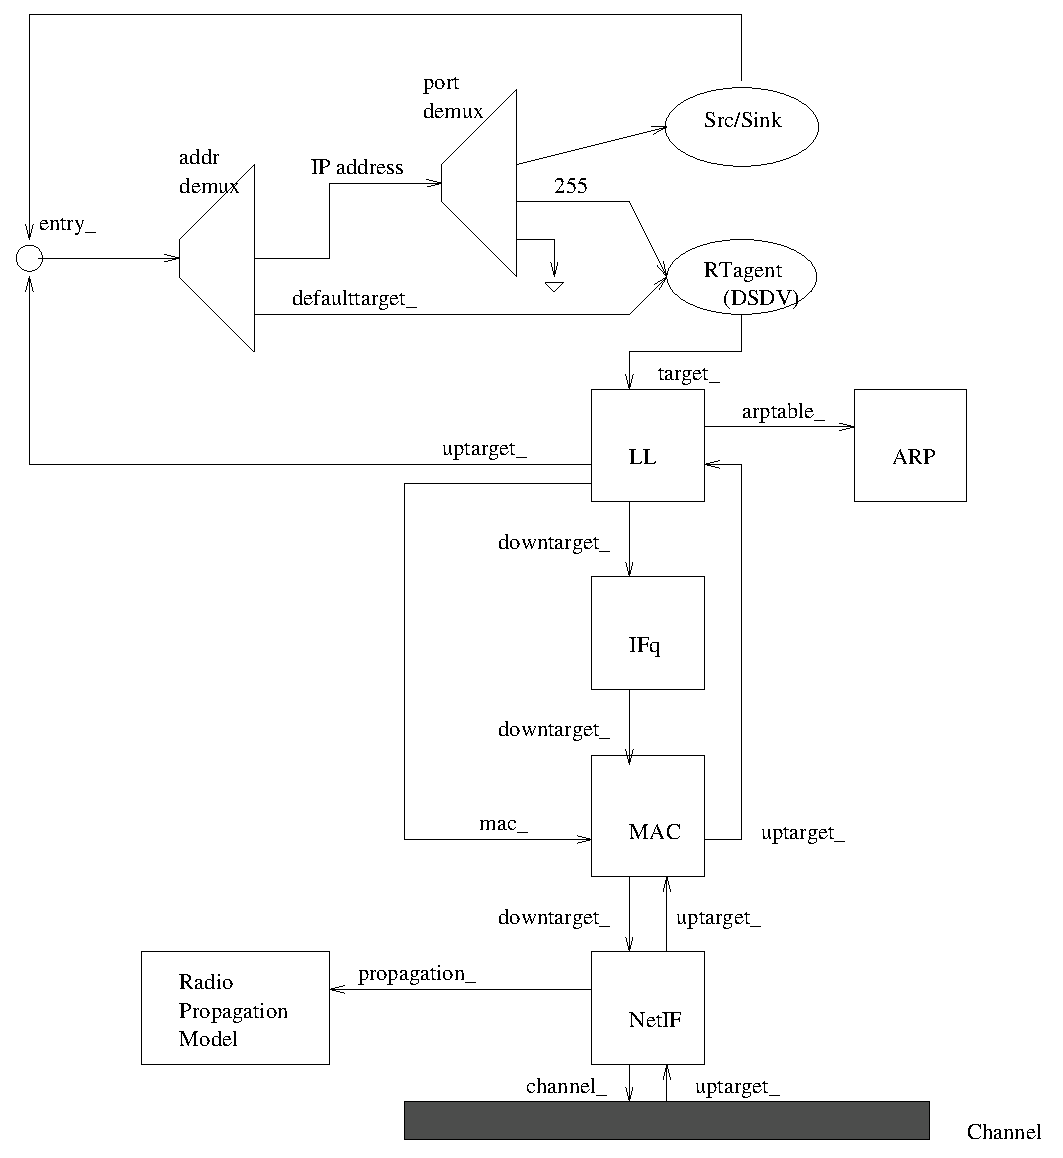
\includegraphics{dsdv}}
    \caption{Schematic of a mobilenode under the CMU monarch's
      wireless extensions to \ns} 
    \label{fig:mobilenode-dsdv} 
\end{figure}

The mobilenode structure used for DSR routing is slightly different from
the mobilenode described above. The class SRNode is derived from class
MobileNode. SRNode doesnot use address demux or classifiers and all
packets received by the node are handed dow   
n to the DSR routing agent by default. The DSR routing agent either
receives pkts for itself by handing it over to the port dmux or forwards
pkts as per source routes in the pkt hdr or sends out route requests and
route replies for fresh packets. Details    
on DSR routing agent may be found in section~\ref{sec:dsr}. The schematic
model for a SRNode is shown in Figure~\ref{fig:mobilenode-dsr}. 
\begin{figure}[tb]
    \centerline{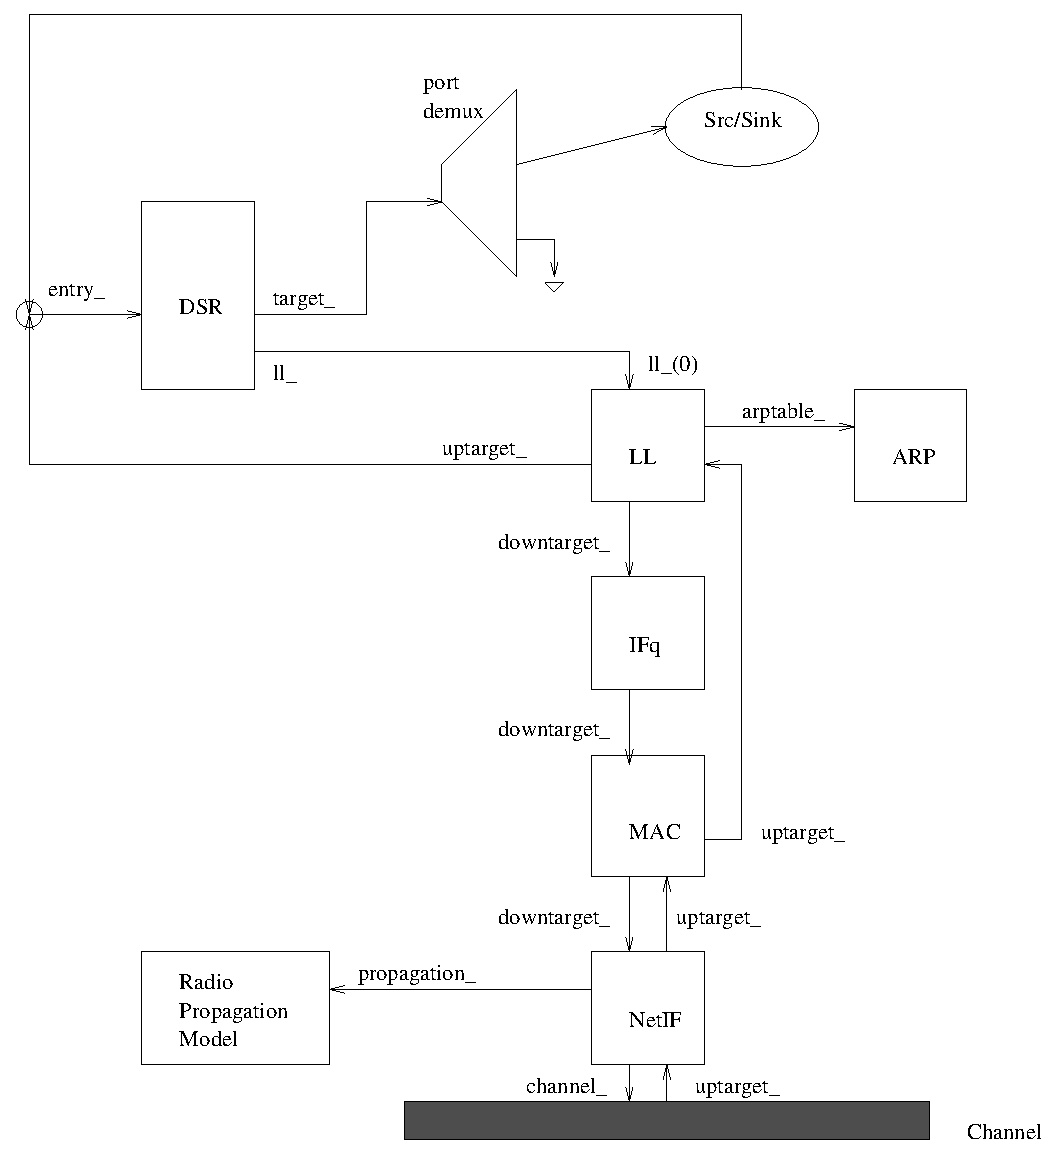
\includegraphics{dsr}}
    \caption{Schematic of a SRNode under the CMU monarch's wireless
      extensions to \ns} 
    \label{fig:mobilenode-dsr}
\end{figure}

\subsection{Creating Node movements}
\label{sec:mobilenode-movements}

The mobilenode is designed to move in a three dimensional topology. However the third dimension (Z) is not used. That is the mobilenode is assumed to move always on a flat terrain with Z always equal to 0.
Thus the mobilenode has X, Y, Z(=0) co-ordinates that is continually adjusted as the node moves. There are two mechanisms to induce movement in mobilenodes. 
In the first method, starting position of the node and its future destinations may be set explicitly. These directives are normally included in a separate movement scenario file. 

The start-position and future destinations for a mobilenode may be set
by using the following APIs:
\begin{program}
$node set X_ <x1>
$node set Y_ <y1>
$node set Z_ <z1>

$ns at $time $node setdest <x2> <y2> <speed> 
\end{program}
At \$time sec, the node would start moving from its initial position 
of (x1,y1) towards a destination (x2,y2) at the defined speed.

In this method the node-movement-updates are triggered whenever the
position of the node at a given time is required to be known. This
may be triggered by a query from a neighbouring node seeking to know
the distance between them, or the setdest directive
described above that changes the direction and speed of the node.

An example of a movement scenario file using the above APIs, can be
found in \nsf{tcl/mobility/scene/scen-670x670-50-600-20-0}. Here
670x670 defines the length and width of the topology with 50 nodes
moving at a maximum speed of 20m/s with average pause time of
600s. These node movement files may be generated using CMU's scenario
generator to be found under
\nsf{indep-utils/cmu-scen-gen/setdest}. See 
subsection~\ref{sec:mobile-scen-generator} for details on generation
of node movement scenarios. 

The second method employs random movement of the node. The primitive
to be used is:
\begin{program}
$mobilenode start
\end{program} %$
which starts the mobilenode with a random position and have routined
updates to change the direction and speed of the node. The destination
and speed values are generated in a random fashion. We have not used
the second method and leave it to the user to 
explore the details. 
The mobilenode movement is implemented in C++. See methods in
\nsf{mobilenode.\{cc.h\}} for the implementational details.

Irrespective of the methods used to generate node movement,
the topography for mobilenodes needs to be defined. It should be
defined before creating mobilenodes. Normally flat topology is created
by specifying the length and width of the topography using the
following primitive:
\begin{program}    
set topo        [new Topography]
$topo load_flatgrid $opt(x) $opt(y)
\end{program} %$
where opt(x) and opt(y) are the boundaries used in simulation.

The movement of mobilenodes may be logged by using a procedure like
the following:

\begin{program}
proc log-movement \{\} \{
    global logtimer ns_ ns

    set ns $ns_
    source ../mobility/timer.tcl
    Class LogTimer -superclass Timer
    LogTimer instproc timeout \{\} \{
        global opt node_;
        for \{set i 0\} \{$i < $opt(nn)\} \{incr i\} \{
            $node_($i) log-movement
        \}
        $self sched 0.1
    \}

    set logtimer [new LogTimer]
    $logtimer sched 0.1
\}
\end{program} %$
In this case, mobilenode positions would be logged every 0.1 sec.

\subsection{Network Components in a mobilenode}
\label{sec:mobilenode-components}

The network stack for a mobilenode consists of a link layer(LL), an
ARP module connected to LL, an interface priority queue(IFq), a mac
layer(MAC), a network interface(netIF), all connected to the channel. 
These network components are created and plumbed together in OTcl. 
The relevant MobileNode method add-interface() in
\nsf{tcl/lib/ns-mobilenode.tcl} is shown below:

\begin{program}
#
#  The following setups up link layer, mac layer, network interface
#  and physical layer structures for the mobile node.
#
Node/MobileNode instproc add-interface \{ channel pmodel 
                lltype mactype qtype qlen iftype anttype \} \{

        $self instvar arptable_ nifs_
        $self instvar netif_ mac_ ifq_ ll_

        global ns_ MacTrace opt

        set t $nifs_
        incr nifs_

        set netif_($t)  [new $iftype]           ;# net-interface
        set mac_($t)    [new $mactype]          ;# mac layer
        set ifq_($t)    [new $qtype]            ;# interface queue
        set ll_($t)     [new $lltype]           ;# link layer
        set ant_($t)    [new $anttype]

        #
        # Local Variables
        #
        set nullAgent_ [$ns_ set nullAgent_]
        set netif $netif_($t)
        set mac $mac_($t)
        set ifq $ifq_($t)
        set ll $ll_($t)

        #
        # Initialize ARP table only once.
        #
        if \{ $arptable_ == "" \} \{
            set arptable_ [new ARPTable $self $mac]
            set drpT [cmu-trace Drop "IFQ" $self]
            $arptable_ drop-target $drpT
        \}

        #
        # Link Layer
        #
        $ll arptable $arptable_
        $ll mac $mac
        $ll up-target [$self entry]
        $ll down-target $ifq

        #
        # Interface Queue
        #
        $ifq target $mac
        $ifq set qlim_ $qlen
        set drpT [cmu-trace Drop "IFQ" $self]
        $ifq drop-target $drpT

        #
        # Mac Layer
        #
        $mac netif $netif
        $mac up-target $ll
        $mac down-target $netif
        $mac nodes $opt(nn)

        #
        # Network Interface
        #
        $netif channel $channel
        $netif up-target $mac
        $netif propagation $pmodel      ;# Propagation Model
        $netif node $self               ;# Bind node <---> interface
        $netif antenna $ant_($t)        ;# attach antenna

        #
        # Physical Channel
        #
        $channel addif $netif           ;# add to list of interfaces

        # ============================================================
        # Setting up trace objects
        
        if \{ $MacTrace == "ON" \} \{
            #
            # Trace RTS/CTS/ACK Packets
            #
            set rcvT [cmu-trace Recv "MAC" $self]
            $mac log-target $rcvT


            #
            # Trace Sent Packets
            #
            set sndT [cmu-trace Send "MAC" $self]
            $sndT target [$mac sendtarget]
            $mac sendtarget $sndT

            #
            # Trace Received Packets
            #
            set rcvT [cmu-trace Recv "MAC" $self]
            $rcvT target [$mac recvtarget]
            $mac recvtarget $rcvT

            #
            # Trace Dropped Packets
            #
            set drpT [cmu-trace Drop "MAC" $self]
            $mac drop-target $drpT
        \} else \{
            $mac log-target [$ns_ set nullAgent_]
            $mac drop-target [$ns_ set nullAgent_]
        \}

        # ============================================================

        $self addif $netif
\}
\end{program} %$

The plumbing in the above method creates the network stack we see in
Figure~\ref{fig:mobilenode-dsdv}.

Each component is briefly described here. Hopefully more detailed
docuentation from CMU shall be available in the future. 
\begin{description}
\item[{\bf Link Layer}] The \code{LL} used by mobilenode is same as
  described in Chapter~\ref{chap:lan}. The only difference being the
  link layer for mobilenode, has an ARP module connected to it which
  resolves all IP to hardware (Mac) address conversions. Normally for
  all outgoing (into the channel) packets, the packets are handed down
  to the \code{LL} by the Routing Agent. The \code{LL} hands down
  packets to the interface queue. For all incoming packets (out of the
  channel), the mac layer hands up packets to the \code{LL} which is
  then handed off at the \code{node_entry_} point. The
  \clsref{LL}{../ns-2/ll.h} is implemented in \nsf{ll.\{cc,h\}} and
  \nsf{tcl/lan/ns-ll.tcl}.

\item [{\bf ARP}] The Address Resolution Protocol (implemented in BSD
  style) module receives queries from Link layer. If ARP has the
  hardware address for destination, it writes it into the mac header
  of the packet. Otherwise it broadcasts an ARP query, and caches the
  packet temporarily. For each unknown destination hardware address,
  there is a buffer for a single packet. Incase additional packets to
  the same destination is sent to ARP, the earlier buffered packet is
  dropped. Once the hardware address of a
  packet"s next hop is known, the packet is inserted into the
  interface queue. The \clsref{ARPTable}{../ns-2/arp.h} is implemented
  in \nsf{arp.\{cc,h\}} and \nsf{tcl/lib/ns-mobilenode.tcl}.

\item[{\bf Interface Queue}] The \clsref{PriQueue}{../ns-2/priqueue.h}
  is implemented as a priority queue which gives priority to routing  
  rotocol packets, inserting them at the head of the queue. It supports
  running a filter over all packets in the queue and removes those with
  a specified destination address. See \nsf{priqueue.\{cc,h\}} for 
  interface queue implementation.

\item[{\bf Mac Layer}] The IEEE 802.11 distributed coordination 
  function (DCF) Mac protocol has been implemented by CMU. It uses a 
  RTS/CTS/DATA/ACK pattern for all unicast packets and simply sends out
  DATA for all broadcast packets. The implementation uses both 
  physical and virtual carrier sense. The
  \clsref{Mac802\_11}{../ns-2/mac-802\_11.h} is implemented in
  \nsf{mac-802\_11.\{cc,h\}}.
  
\item[{\bf Tap Agents}] \code{Agents} that subclass themselves as
  \clsref{Tap}{../ns-2/mac.h} defined in mac.h can register themselves
  with the mac object using method installTap(). If the particular Mac
  protocol permits it, the tap will promiscuously be 
  given all packets received by the mac layer, before address filtering
  is done. See \nsf{mac.\{cc,h\}} for \clsref{Tap} implementation. 

\item[{\bf Network Interfaces}] The Network Interphase layer serves as
  a hardware interface which is used by mobilenode to access the
  channel. The wireless shared media interface is implemented as
  \clsref{Phy/WirelessPhy}{../ns-2/wireless-phy.h}. This interface
  subject to collisions and the radio propagation model receives
  packets transmitted by other node interfaces to the channel. The
  interface stamps each transmitted packet with the meta-data related
  to the transmitting interface like the transmission power,
  wavelength etc. This meta-data in pkt header is used by the
  propagation model in receiving network interface to determine if the
  packet has minimum power to be received and/or captured and/or
  detected (carrier sense) by the receiving node. The model
  approximates the DSSS radio interface (Lucent WaveLan
  direct-sequence spread-spectrum). See \nsf{phy.\{cc.h\}} and
  \nsf{wireless-phy.\{cc,h\}} for network interface implementations.

\item[{\bf Radio Propagation Model}]  It uses Friss-space attenuation
  ($1/r^2$) at near distances and an approximation to Two ray Ground
  ($1/r^4$) at far distances. The approximation assumes specular
  reflection off a flat ground plane. See \nsf{tworayground.\{cc,h\}}
  for implementation.

\item[{\bf Antenna}] An omni-directional antenna having unity gain is 
  used by mobilenodes. See \nsf{antenna.\{cc,h\}} for implementation
  details. 
\end{description}

\subsection{Different types of Routing Agents in mobile networking}
\label{sec:mobilenode-routing}

The four different ad-hoc routing protocols currently implemented
for mobile networking in \ns are dsdv, dsr, aodv and tora. In this section
we shall briefly discuss each of them.

\subsubsection{DSDV}
\label{sec:dsdv}

In this routing protocol routing messages are exchanged between
neighbouring mobilenodes (i.e mobilenodes that are within range of one
another). Routing updates may be triggered or routine. Updates are
triggered in case a routing information from one of t   
he neighbours forces a change in the routing table.
A packet for which the route to its destination is not known is cached
while routing queries are sent out. The pkts are cached until
route-replies are received from the destination. There is a maximum buffer
size for caching the pkts waiting for routing information beyond which
pkts are dropped. 

All packets destined for the mobilenode are routed directly by the address
dmux to its port dmux. The port dmux hands the packets to the respective
destination agents. A port number of 255 is used to attach routing agent
in mobilenodes. The mobilenodes al
so use a default-target in their classifier (or address demux). In the
event a target is not found for the destination in the classifier (which
happens when the destination of the packet is not the mobilenode itself),
the pkts are handed to the default-ta   
rget which is the routing agent. The routing agent assigns the next hop
for the packet and sends it down to the link layer. 

The routing protocol is mainly implemented in C++. See \nsf{dsdv}
directory and \nsf{tcl/mobility/dsdv.tc}l for all procedures related to
DSDV protocol implementation.  

\subsubsection{DSR}
\label{sec:dsr}

This section briefly describes the functionality of the dynamic source
routing protocol. As mentioned earlier the \code{SRNode} is different from
the \code{MobileNode}.  The \code{SRNode}'s \code{entry\_} points to the
DSR routing agent, thus forcing all    
packets received by the node to be handed down to the routing agent. This
model is required for future implementation of piggy-backed routing
information on data packets which otherwise would not flow through the
routing agent.   

The DSR agent checks every data packet for source-route information. It
forwards the packet as per the routing information. Incase it doesnot find
routing information in the packet, it provides the source route, if route
is known, or caches the packet and   
sends out route queries if route to destination is not known. Routing
queries, always triggered by a data packet with no route to its
destination, are initially broadcast to all neighbours. Route-replies are
send back either by intermediate nodes or the 
destination node, to the source, if it can find routing info for the
destination in the route-query.  It hands over all packets destined to
itself to the port dmux.  
In \code{SRNode} the port number 255 points to a null agent since the
packet has already been processed by the routing agent. 

See \nsf{dsr} directory and \nsf{tcl/mobility/dsr.tcl} for implementation
of DSR protocol. 

\subsubsection{TORA}
\label{sec:tora}

Tora is a distributed routing protocol based on "link reversal" algorithm. 
At every node a separate copy of TORA is run for every destination. When a
node needs a route to a given destination it broadcasts a QUERY message
containing the address of the destination for which it requires  a route.
This packet travels through the network until it reaches the destination
or an intermediate node that has a route to the destination node.
This recepient node node then broadcasts an UPDATE packet listing its
height wrt the destination. As this node propagates through the network
each node updates its height to a value greater than the height of the
neighbour from which it receives the UPDATE. This results in a series of
directed links from the node that originated the QUERY to the destination
node. If a node discovers a particular destination to be unreachable it
sets a local maximum value of height for that destination. Incase the node
cannot find any neighbour having finite height wrt this destination it
attempts to find a new route. In case of network partition, the node
broadcasts a CLEAR message that resets all routing states and removes
invalid routes from the network.

TORA operates on top of IMEP (Internet MANET Encapsulation Protocol) that
provides reliable delivery of route-messages and informs the routing
protocol of any changes of the links to its neighbours. IMEP tries to
aggregate IMEP and TORA messages into a single packet (called block) in
order to reduce overhead. For link-status sensing and maintaining a list
of neighbour nodes, IMEP sends out periodic BEACON messages which is
answered by each node that hears it by a HELLO reply message.
See \ns/tora directory and \ns/tcl/mobility/tora.tcl for implementation of
tora in \ns.

\subsubsection{AODV}
\label{sec:AODV}

AODV is a combination of both DSR and DSDV protocols. It has the basic
route-discovery and route-maintenance of DSR and uses the hop-by-hop
routing, sequence numbers and beacons of DSDV. The node that wants to know
a route to a given destination generates a ROUTE REQUEST. The route
request is forwarded by intermediate nodes that also creates a reverse
route for itself from the destination. When the request reaches a node
with route to destination it generates a ROUTE REPLY containing the number
of hops requires to reach destination. All nodes that participates in
forwarding this reply to the source node creates a forward route to
destination. This state created from each node from source to destination
is a hop-by-hop state and not the entire route as is done in source
routing.
See \ns/aodv and \ns/tcl/lib/ns-lib.tcl for implementational details
of aodv.


\subsection{Trace Support}
\label{sec:mobile-trace}

The trace support for wireless simulations currently use cmu-trace
objects. In the future this shall be extended to merge with trace and
monitoring support available in ns, which would also include nam support
for wireless modules. For now we will explain briefly with cmu-trace
objects and how they may be used to trace packets for wireless scenarios. 

The cmu-trace objects are of three types - \code{CMUTrace/Drop},
\code{CMUTrace/Recv} and \code{CMUTrace/Send}. These are used for tracing
packets that are dropped, received and sent by agents, routers, mac layers
or interface queues in \ns. The methods and procedures used for
implementing wireless trace support can be found under
\nsf{trace.\{cc,h\}} and \nsf{tcl/lib/ns-cmutrace.tcl}.

A cmu-trace object may be created by the following API:
\begin{program}
set sndT [cmu-trace Send "RTR" $self]
\end{program} %$
which creates a trace object, sndT, of the type \code{CMUTrace/Send}
for tracing all packets that are sent out in a router. The trace
objects may be used to trace packets in MAC, agents (routing or
others), routers or any other NsObject. 

The cmu-trace object \code{CMUTrace} is derived from the base class
\code{Trace}. See Chapter~\ref{chap:trace} for details on class
\code{Trace}. The class \code{CMUTrace} is defined as the following:

\begin{program}
class CMUTrace : public Trace \{
public:
        CMUTrace(const char *s, char t);
        void    recv(Packet *p, Handler *h);
        void    recv(Packet *p, const char* why);

private:
        int off_arp_;
        int off_mac_;
        int off_sr_;

        char    tracename[MAX_ID_LEN + 1];
        int     tracetype;
        MobileNode *node_;

        int initialized() \{ return node_ && 1; \}

        int     command(int argc, const char*const* argv);
        void    format(Packet *p, const char *why);

        void    format_mac(Packet *p, const char *why, int offset);
        void    format_ip(Packet *p, int offset);

        void    format_arp(Packet *p, int offset);
        void    format_dsr(Packet *p, int offset);
        void    format_msg(Packet *p, int offset);
        void    format_tcp(Packet *p, int offset);
        void    format_rtp(Packet *p, int offset);
\};
\end{program}

The type field (described in \code{Trace} class definition) is used to
differentiate among different types of traces. For cmu-trace this can be
{\bf s} for sending, {\bf r} for receiving or {\bf D} for dropping a
packet. A fourth type {\bf f} is used to denote forwarding of a packet
(When the node is not the originator of the packet). 
Similar to the method Trace::format(), the CMUTrace::format() defines and
dictates the trace file format. The method is shown below: 
\begin{program}
void CMUTrace::format(Packet* p, const char *why)
\{
        hdr_cmn *ch = HDR_CMN(p);
        int offset = 0;

        /*
         * Log the MAC Header
         */
        format_mac(p, why, offset);
        offset = strlen(wrk_);

        switch(ch->ptype()) \{

        case PT_MAC:
                break;

        case PT_ARP:
                format_arp(p, offset);
                break;

        default:
                format_ip(p, offset);
                offset = strlen(wrk_);

                switch(ch->ptype()) \{

                case PT_DSR:
                        format_dsr(p, offset);
                        break;

                case PT_MESSAGE:
                case PT_UDP:
                        format_msg(p, offset);
                        break;
                        
                case PT_TCP:
                case PT_ACK:
                        format_tcp(p, offset);
                        break;
                        
                case PT_CBR:
                        format_rtp(p, offset);
                        break;
                ..........

                \}
        \}
\}
\end{program}
The above function calls different format functions depending on the type
of the packet being traced. All traces are written to the buffer wrk\_. A
count of the offset for the buffer is kept and is passed along the
different trace functions. The most basic format is defined by
format\_mac() and is used to trace all pkt types. The other format
functions print additional information as defined by the packet types. The
mac format prints the following:   
\begin{program}
\#ifdef LOG_POSITION
        double x = 0.0, y = 0.0, z = 0.0;
        node_->getLoc(&x, &y, &z);
\#endif

        sprintf(wrk_ + offset,
\#ifdef LOG_POSITION
                "%c %.9f %d (%6.2f %6.2f) %3s %4s %d %s %d [%x %x %x %x] ",
\#else
                "%c %.9f _%d_ %3s %4s %d %s %d [%x %x %x %x] ",
\#endif
                op,                    // s, r, D or f
                Scheduler::instance().clock(),  // time stamp
                src_,                  // the nodeid for this node
\#ifdef LOG_POSITION
                x,                     // x co-ord 
                y,                     // y co-ord
\#endif
                tracename,             // name of object type tracing
                why,                   // reason, if any

                ch->uid(),             // identifier for this event
                packet_info.name(ch->ptype()), // packet type
                ch->size(),                    // size of cmn header
                mh->dh_duration,       // expected time to send data 
                ETHER_ADDR(mh->dh_da), // mac_destination address
                ETHER_ADDR(mh->dh_sa),         // mac_sender address
                GET_ETHER_TYPE(mh->dh_body));  // type - arp or IP
\end{program}

If the LOG\_POSITION is defined the x and y co-ordinates for the
mobilenode is also printed. The descriptions for different fields in the
mac trace are given in the comments above. For all IP packets additional
IP header fields are also added to the above trace. The IP trace is
described below:

\begin{program}
sprintf(wrk_ + offset, "------- [%d:%d %d:%d %d %d] ",
                src,          // IP src address
                ih->sport_,   // src port number
                dst,          // IP dest address
                ih->dport_,   // dest port number
                ih->ttl_,     // TTL value 
                (ch->next_hop_ < 0) ? 0 : ch->next_hop_); // next hopaddress, if any.
\end{program}

An example of a trace for a tcp packet is as follows:
\begin{program}
r 160.093884945 _6_ RTR  --- 5 tcp 1492 [a2 4 6 800] ------- [655
36:0 16777984:0 31 16777984] [1 0] 2 0
\end{program}
Here we see a TCP data packet being received by a node with id of 6. UID
of this pkt is 5 with a cmn hdr size of 1492. The mac details shows an IP
pkt (ETHERTYPE\_IP is defined as 0x0800, ETHERTYPE\_IP is 0x0806 ), mac-id
of this receiving node is 6. That of the sending node is 4 and expected
time to send this data pkt over the wireless channel is a2 (hex2dec
conversion: 160+2 sec). Additionally, IP traces information about IP src
and destination addresses. The src translates (using a 3 level
hier-address of 8/8/8) to a address string of 0.1.0 with port of 0. The
dest address is 1.0.3 with port address of 0. The TTL value is 31 and the
destination was a hop away from the src. Additionally TCP format prints
information about tcp seqno of 1, ackno of 0. See other formats described
in \nsf/cmu-trace.cc for DSR, UDP/MESSAGE, TCP/ACK and CBR packet types.

Other trace formats are also used by the routing agents (TORA and DSR) to
log certain special routing events like "originating" (adding a SR header
to a packet) or  "ran off the end of a source route" indicating some sort
of routing problem with the source route etc. These special event traces
begin with "S" for DSR and "T" for Tora and may
be found in \nsf{tora/tora.cc} for TORA and \nsf{dsr/dsrgent.cc} for DSR
routing agent.


\subsection{Revised format for wireless traces}
\label{sec:revtraceformat}

In an effort to merge wireless trace, using cmu-trace objects, with
ns tracing, a new, inproved trace format has been introduced. This revised
trace support is backwards compatible with the old trace formatting and
can be enabled by the following command:
\begin{program}
$ns use-newtrace
\end{program}
This command should be called before the universal trace command \code{$ns
trace-all <trace-fd>}. Primitive \code{use-newtrace} sets up new
format for wireless tracing by setting a simulator variable called
\code{newTraceFormat}. Currently this new trace support is available for
wireless simulations only and shall be extended to rest of \ns in the near
future.

An example of the new trace format is shown below:
\begin{program}
s -t 0.267662078 -Hs 0 -Hd -1 -Ni 0 -Nx 5.00 -Ny 2.00 -Nz 0.00 -Ne
-1.000000 -Nl RTR -Nw --- -Ma 0 -Md 0 -Ms 0 -Mt 0 -Is 0.255 -Id -1.255 -It
message -Il 32 -If 0 -Ii 0 -Iv 32
s -t 1.511681090 -Hs 1 -Hd -1 -Ni 1 -Nx 390.00 -Ny 385.00 -Nz 0.00 -Ne
-1.000000 -Nl RTR -Nw --- -Ma 0 -Md 0 -Ms 0 -Mt 0 -Is 1.255 -Id -1.255 -It
message -Il 32 -If 0 -Ii 1 -Iv 32
s -t 10.000000000 -Hs 0 -Hd -2 -Ni 0 -Nx 5.00 -Ny 2.00 -Nz 0.00 -Ne
-1.000000 -Nl AGT -Nw --- -Ma 0 -Md 0 -Ms 0 -Mt 0 -Is 0.0 -Id 1.0 -It tcp -Il 1000 -If
2 -Ii 2 -Iv 32 -Pn tcp -Ps 0 -Pa 0 -Pf 0 -Po 0
r -t 10.000000000 -Hs 0 -Hd -2 -Ni 0 -Nx 5.00 -Ny 2.00 -Nz 0.00 -Ne
-1.000000 -Nl RTR -Nw --- -Ma 0 -Md 0 -Ms 0 -Mt 0 -Is 0.0 -Id 1.0 -It tcp -Il 1000 -If
2 -Ii 2 -Iv 32 -Pn tcp -Ps 0 -Pa 0 -Pf 0 -Po 0
r -t 100.004776054 -Hs 1 -Hd 1 -Ni 1 -Nx 25.05 -Ny 20.05 -Nz 0.00 -Ne
-1.000000 -Nl AGT -Nw --- -Ma a2 -Md 1 -Ms 0 -Mt 800 -Is 0.0 -Id 1.0 -It
tcp -Il 1020 -If 2 -Ii 21 -Iv 32 -Pn tcp -Ps 0 -Pa 0 -Pf 1 -Po 0
s -t 100.004776054 -Hs 1 -Hd -2 -Ni 1 -Nx 25.05 -Ny 20.05 -Nz 0.00 -Ne
-1.000000 -Nl AGT -Nw --- -Ma 0 -Md 0 -Ms 0 -Mt 0 -Is 1.0 -Id 0.0 -It ack -Il 40
-If 2 -Ii 22 -Iv 32 -Pn tcp -Ps 0 -Pa 0 -Pf 0 -Po 0 
\end{program}

\subsubsection{Explanation of new trace format}
The new trace format as seen above can be can be divided into the
following fields :
\begin{description}
\item[Event type]
In the traces above, the first field (as in the older trace format)
describes the type of event taking place at the node and can be one of the 
four types:
\begin{description}
\item[s] send 
\item[r] receive 
]item[d] drop 
\item[f] forward
\end{description}

\item[General tag]
The second field starting with "-t" may stand for time or global setting
\begin{description}
\item[-t] time
\item[-t] * (global setting)
\end{description}

\item[Node property tags]
This field denotes the node properties like node-id, the level at
which tracing is being done like agent, router or MAC. The tags start
with a leading "-N" and are listed as below:
\begin{description}
\item[-Ni:] node id
\item[-Nx:] node's x-coordinate
\item[-Ny:] node's y-coordinate
\item[-Nz:] node's z-coordinate
\item[-Ne:] node energy level
\item[-Nl:] trace level, such as AGT, RTR, MAC
\item[-Nw:] reason for the event. The different reasons for dropping a
packet are given below:
\begin{description}
\item["END"] DROP\_END\_OF\_SIMULATION          
\item["COL"] DROP\_MAC\_COLLISION              
\item["DUP"] DROP\_MAC\_DUPLICATE 
\item["ERR"] DROP\_MAC\_PACKET\_ERROR  
\item["RET"] DROP\_MAC\_RETRY\_COUNT\_EXCEEDED
\item["STA"] DROP\_MAC\_INVALID\_STATE      
\item["BSY"] DROP\_MAC\_BUSY                 

\item["NRTE"] DROP\_RTR\_NO\_ROUTE i.e no route is available.
\item["LOOP"] DROP\_RTR\_ROUTE\_LOOP i.e there is a routing loop
\item["TTL"]  DROP\_RTR\_TTL i.e TTL has reached zero.
\item["TOUT"] DROP\_RTR\_QTIMEOUT i.e packet has expired.
\item["CBK"]  DROP\_RTR\_MAC\_CALLBACK

\item["IFQ"]  DROP\_IFQ\_QFULL i.e no buffer space in IFQ.
\item["ARP"]  DROP\_IFQ\_ARP\_FULL i.e dropped by ARP
\item["OUT"]  DROP\_OUTSIDE\_SUBNET i.e dropped by base stations on
receiving routing updates from nodes outside its domain.
\end{description}
\end{description}

\item[Packet information at IP level]
The tags for this field start with a leading "-I" and are listed along
with their explanations as following:
\begin{description}
\item[-Is:] source address.source port number
\item[-Id:] dest address.dest port number
\item[-It:] packet type
\item[-Il:] packet size
\item[-If:] flow id
\item[-Ii:] unique id
\item[-Iv:] ttl value  
\end{description}

\item[Next hop info]
This field provides next hop info and the tag starts with a leading "-H".
\begin{description}
\item[-Hs:] id for this node
\item[-Hd:] id for next hop towards the destination.
\end{description}

\item[Packet info at MAC level]
This field gives MAC layer information and starts with a leading "-M" as
shown below:
\begin{description}
\item[-Ma:] duration
\item[-Md:] dst's ethernet address
\item[-Ms:] src's ethernet address
\item[-Mt:] ethernet type  
\end{description}     

\item[Packet info at "Application level"]
The packet information at application level consists of the type of
application like ARP, TCP, the type of adhoc routing protocol like
DSDV, DSR, AODV etc being traced. This field consists of a leading "-P"
and list of tags for different application is listed as below:
\begin{description}
\item[-P arp] Address Resolution Protocol. Details for ARP is given by the
following tags:
\begin{description}
\item[-Po:] ARP Request/Reply
\item[-Pm:] src mac address
\item[-Ps:] src address
\item[-Pa:] dst mac address
\item[-Pd:] dst address
\end{description}

\item[-P dsr] This denotes the adhoc routing protocol called Dynamic
source routing. Information on DSR is represented by the following tags:
\begin{description}
\item[-Pn:] how many nodes traversed
\item[-Pq:] routing request flag
\item[-Pi:] route request sequence number
\item[-Pp:] routing reply flag
\item[-Pl:] reply length
\item[-Pe:] src of srcrouting->dst of the source routing
\item[-Pw:] error report flag ?
\item[-Pm:] number of errors
\item[-Pc:] report to whom
\item[-Pb:] link error from linka->linkb
\end{description}

\item[-P cbr] Constant bit rate. Information about the CBR application is
represented by the following tags:

\begin{description}
\item[-Pi:] sequence number
\item[-Pf:] how many times this pkt was forwarded
\item[-Po:] optimal number of forwards 
\end{description}

\item[-P tcp] Information about TCP flow is given by the following
subtags:

\begin{description}
\item[-Ps:] seq number
\item[-Pa:] ack number
\item[-Pf:] how many times this pkt was forwarded
\item[-Po:] optimal number of forwards 
\end{description}
\end{description}

This field is still under development and new tags shall be added for
other applications as they get included along the way.
\end{description}


\subsection{Generation of node-movement and traffic-connection for
  wireless scenarios}
\label{sec:mobile-scen-generator}

Normally for large topologies, the node movement and traffic connection
patterns are defined in separate files for convinience. These movement and
traffic files may be generated using CMU's movement- and
connection-generators. In this section we shall describe both separately.

\subsubsection{MobileNode Movement}
\label{sec:mobile-movement-file}

Some examples of node movement files may be found in
\nsf{tcl/mobility/scene/scen-670x670-50-600-20-\{0,1,2\}. These files
define a topology of 670 by 670m where 50 nodes move with a speed of 20m/s
with pause time of 600s. each node is assigned a starting position. The
information regarding number of hops between the nodes is fed to the
central object "GOD" (XXX but why/where is this information used??-answer
awaited from CMU.) Next each node is a speed and a direction to move to. 

The generator for creating node movement files are to be found under
\nsf{indep-utils/cmu-scen-gen/setdest/} directory. Compile the files
under setdest to create an executable. run setdest with arguments in
the following way:
\begin{program}
./setdest -n <num_of_nodes> -p <pausetime> -s <maxspeed> -t <simtime>
          -x <maxx> -y <maxy> > <outdir>/<scenario-file>
\end{program}
Note that the index used for nodes now start from 0 instead of 1 as
was in the original CMU version, to match with \ns's tradition of
assigning node indices from 0.


\subsubsection{Generating traffic pattern files}
\label{sec:mobile-traffic-file}

The examples for traffic patterns may be found in
\nsf{tcl/mobility/scene/cbr-50-\{10-4-512, 20-4-512\}}.

The traffic generator is located under \nsf{indep-utils/cmu-scen-gen/}
and are called cbrgen.tcl and tcpgen.tcl. They may be used for
generating CBR and TCP connections respectively.

To create CBR connecions, run
\begin{program}
ns cbrgen.tcl [-type cbr|tcp] [-nn nodes] [-seed seed] 
              [-mc connections] [-rate rate]
\end{program}
To create TCP connections, run
\begin{program}
ns tcpgen.tcl [-nn nodes] [-seed seed]
\end{program}
You will need to pipe the outputs from above to a cbr-* or a tcp-* file.


\section{Extensions made to CMU's wireless model}
\label{sec:wireless-extensions}

As mentioned earlier, the original CMU wireless model allows
simulation of wireless LANs and ad-hoc networks. However in order to
use the wireless model for simulations using both wired and wireless
nodes we had to add certain extensions to cmu model. We 
call this wired-cum-wireless feature. Also SUN's MobileIP (implemented
for wired nodes) was integrated into the wireless model allowing
mobileIP to run over wireless mobilenodes. The following two
subsections describe these two extensions to the wireless 
model in \ns. 


\subsection{wired-cum-wireless scenarios}
\label{sec:wired-cum-wireless}

The mobilenodes described so far mainly supports simulation of
multi-hop ad-hoc networks or wireless LANs. But what if we need to
simulate a topology of multiple wireless LANs connected through wired
nodes, or may need to run mobileIP on top of these wireless nodes? The
extensions made to the CMU wireless model allows us to do that. 

The main problem facing the wired-cum-wireless scenario was the issue
of routing. In ns, routing information is generated based on the
connectivity of the topology, i.e how nodes are connected to one
another through \code{Links}. Mobilenodes on the other hand have no
concept of links. They route packets among themselves, within the
wireless topology, using their routing protocol. so how would packets
be exchanged between these two types of nodes? 

So a node called \code{BaseStationNode} is created which plays the
role of a gateway for the wired and wireless domains. The
\code{BaseStationNode} is essentially a hybrid between a Hierarchical
node\footnote{Refer to Chapter~\ref{chap:hier-rtg} for details on
  hierarchical routing and internals of \code{HierNode}.}
(\code{HierNode}) and a \code{MobileNode}. The basestation node is
responsible for delivering packets into and out of the wireless
domain. In order to achieve this we need Hierarchical routing. 

Each wireless domain along with its base-station would have an unique
domain address assigned to them. All packets destined to a wireless
node would reach the base-station attached to the domain of that
wireless node, who would eventually hand the packet
over to the destination (mobilenode). And mobilenodes route packets,
destined to outside their (wireless) domain, to their base-station
node. The base-station knows how to forward these packets towards the
(wired) destination.
\begin{figure}
    \centerline{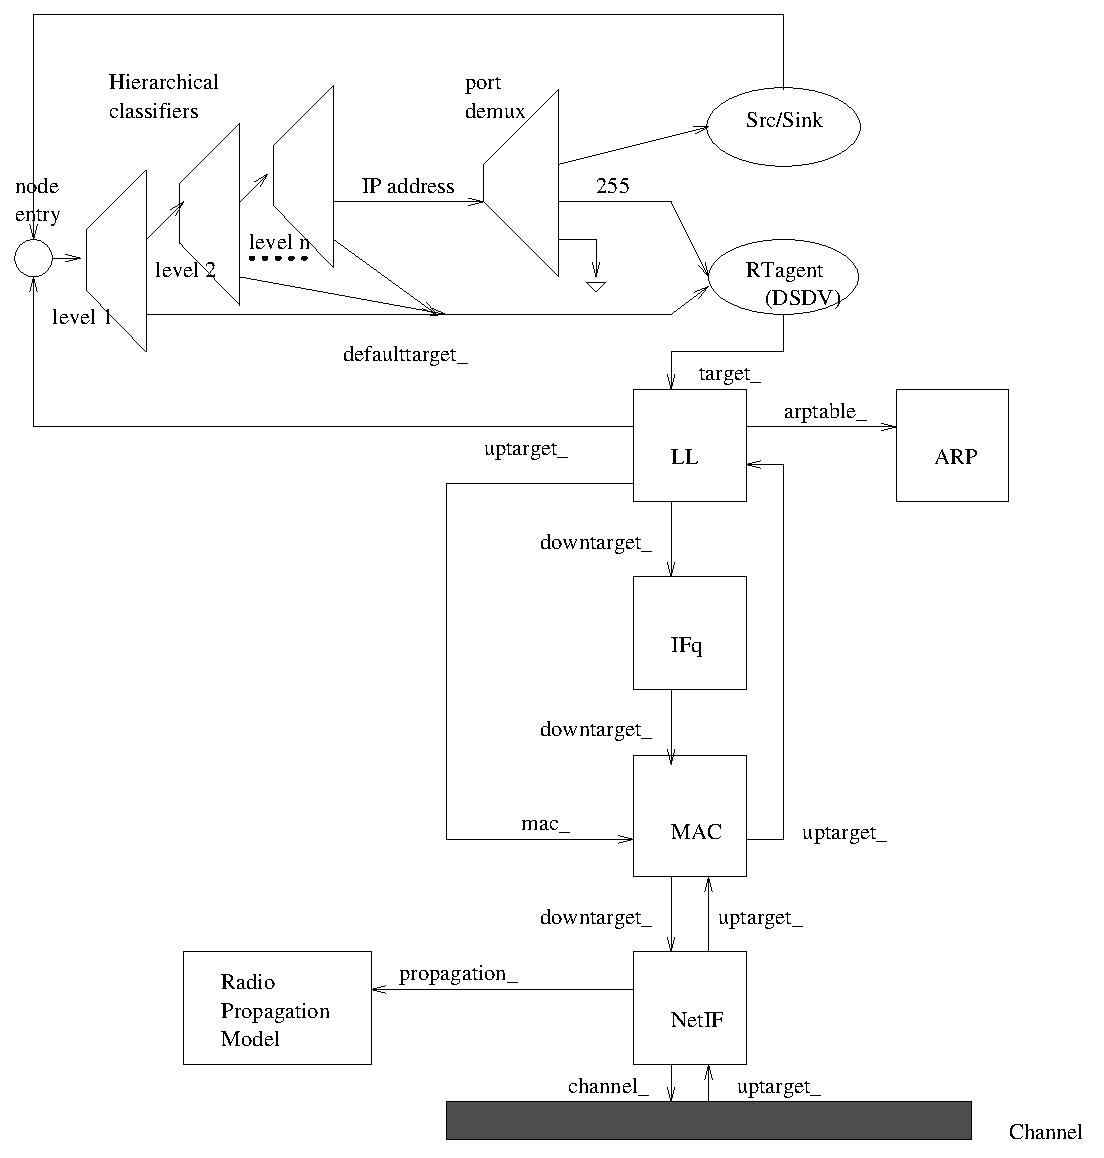
\includegraphics{basestation}}
    \caption{Schematic of a baseStationNode}
    \label{fig:mobilenode-basestation}
\end{figure}
The schematic of a \code{BaseStationNode} is shown in
Figure~\ref{fig:mobilenode-basestation}.

The mobilenodes in wired-cum-wireless scenario are required to support
hierarchical addressing/routing. Thus the \code{MobileNode} looks
exactly like the \code{BaseStationNode}. The SRNode, however, simply
needs to have its own hier-address since it does not require any
address demuxes and thus is not required to support hier
routing\footnote{In order to do away with all these different
  variations of the definition of a node, we are planning to revise
  the node architecture that would allow a more flexible
  and modularised construction of a node without the necessity of having
  to define and be limited to certain Class definitions only.}.

The DSDV agent on having to forward a packet checks to see if the
destination is outside its (wireless) subnet. If so, it tries to
forward the packet to its base-station node. In case no route to
base-station is found the packet is dropped. Otherwise the
packet is forwarded to the next\_hop towards the base-station. Which
is then routed towards the wired network by base-station's
classifiers.

The DSR agent, on receiving a pkt destined outside its subnet, sends
out a route-query for its base-station in case the route to
base-station is not known. The data pkt is temporarily cached while it
waits to hear route replies from base-station. On getting a reply the
packet is provided with routing information in its header and send
away towards the base-station. The base-station address demuxes routes
it correctly toward the wired network.

The example script for a wired-cum-wireless simulation can be found at
\nsf{tcl/ex/wired-cum-wireless-sim.tcl}. The methods for
wired-cum-wireless implementations are defined in
\nsf{tcl/lib/ns-bsnode.tcl}, \nsf{tcl/mobility/\{com.tcl,dsr.tcl,
  dsdv.tcl\}}, \nsf{dsdv/dsdv.\{cc,h\}} and
\nsf{dsr/dsragent.\{cc,h\}}.


\subsection{MobileIP}
\label{sec:mobileip}

The wired-cum-wireless extensions for the wireless model paved the
path for supporting wireless MobileIP in \ns. Sun Microsystem's
(Charlie Perkins {\em et al}) MobileIP model was based on ns's wired model
(consisting of \code{Node}'s and \code{Link}'s) and thus didnot use
CMU's mobility model.

Here we briefly describe the wireless MobileIP implementation. We hope
that Sun would provide the detailed version of the documentation in
the future.

The mobileIP scenario consists of Home-Agents(HA) and
Foreign-Agents(FA) and have Mobile-Hosts(MH) moving between their HA
and FAs.
The HA and FA are essentially base-station nodes we have described
earlier. While MHs are basically the mobileNodes described in
section~\ref{sec:mobilenode-creation}.
The methods and procedures for MobileIP extensions are described in
\nsf{mip.\{cc,h\}}, \nsf{mip-reg.cc}, \nsf{tcl/lib/ns-mip.tcl} and
\nsf{tcl/lib/ns-wireless-mip.tcl}.

\begin{figure}
    \centerline{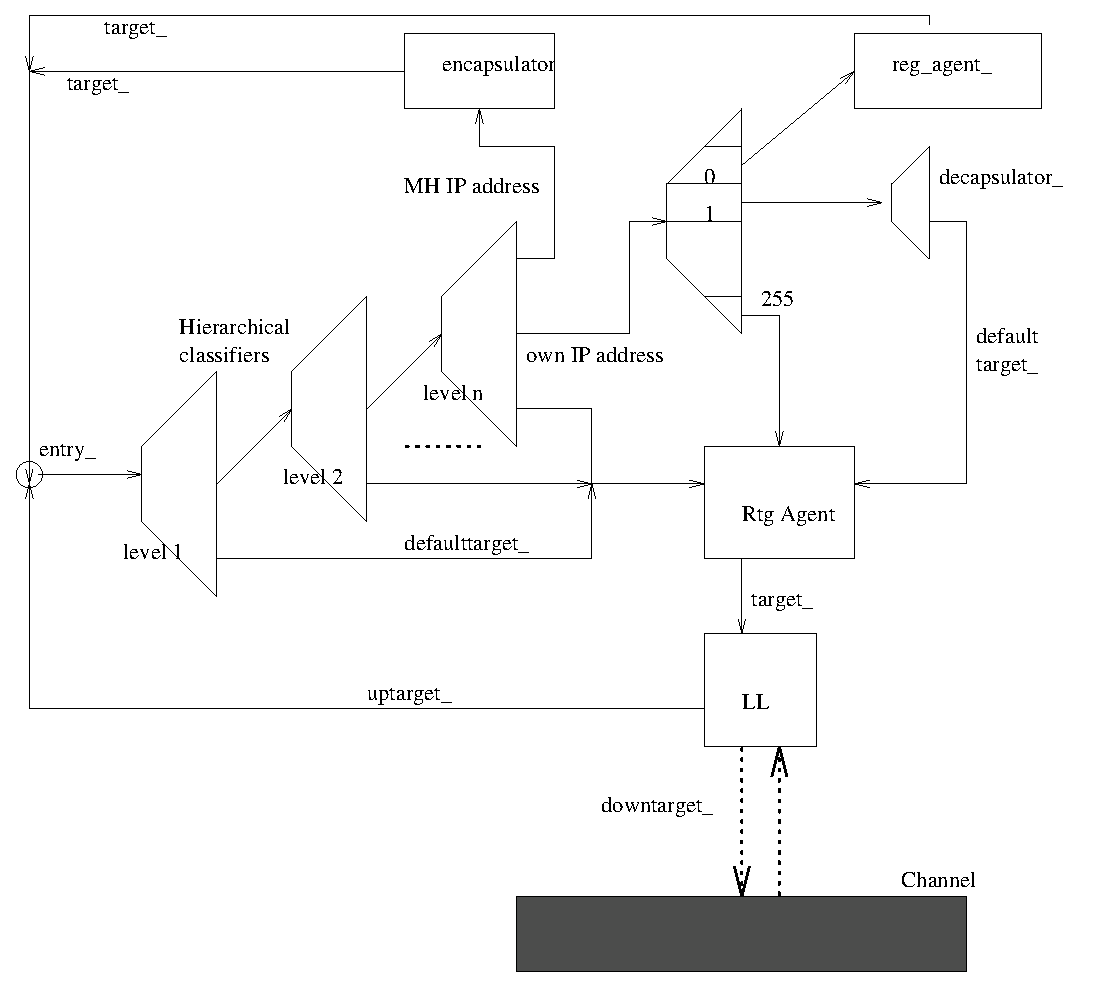
\includegraphics{wireless-mip}}
    \caption{Schematic of a Wireless MobileIP BaseStation Node}
    \label{fig:mobilenode-wireless-mip}
\end{figure}
The HA and FA nodes are defined as \code{MobileNode/MIPBS} having a
registering agent (regagent\_) that sends beacon out to the
mobilenodes, sets up encapsulator and decapsulator, as required and
replies to solicitations from MHs. 
The MH nodes are defined as \code{MobileNode/MIPMH} which too have a
regagent\_ that receives and responds to beacons and sends out
solicitations to HA or FAs. Figure~\ref{fig:mobilenode-wireless-mip}
illustrates the schematic of a \code{MobileNode/MIPBS} 
node. The \code{MobileNode/MIPMH} node is very similar to this except
for the fact that it doesnot have any encapsulator or decapsulator. As
for the SRNode version of a MH, it doesnot have the hierarchical
classifiers and the RA agent forms the entry point of the node. See
Figure~\ref{fig:mobilenode-dsr} for model of a SRNode. 

The \code{MobileNode/MIPBS} node routinely broadcasts beacon or
advertisement messages out to MHs. A solicitation from a mobilenode
generates an ad that is send directly to the requesting MH. The
address of the base-station sending out beacon is heard by 
MH and is used as the COA (care-of-address) of the MH. Thus as the MH
moves from its native to foreign domains, its COA changes. 
Upon receiving  reg\_request (as reply to ads) from a mobilehost the
base-station checks to see if it is the HA for the MH. If not, it sets
up its decapsulator and forwards the reg\_request towards the HA of
the MH. 

In case the base-station {\em is} the HA for the requesting MH but the
COA doesnot match its own, it sets up an encapsulator and sends
reg-request-reply back to the COA (address of the FA) who has
forwarded the reg\_request to it. so now all packets destined to the
MH reaching the HA would be tunneled through the encapsulator which
encapsulates the IP pkthdr with a IPinIP hdr, now destined to the COA
instead of MH. The FA's decapsulator recives this packet, removes the
encapsulation and sends it to the MH.

If the COA matches that of the HA, it just removes the encapsulator it
might have set up (when its mobilehost was roaming into foreign
networks) and sends the reply directly back to the MH, as the MH have
now returned to its native domain.

The mobilehost sends out solicitations if it doesnot hear any ads from the
base-stations. Upon receiving ads, it changes its COA to the address of
the HA/FA it has heard the ad from, and replies back to the COA with a
request for registration (\code{reg-request}).
Initially the MH maybe in the range of the HA and receives all pkts
directly from its COA which is HA in this case. 
Eventually as the MH moves out of range of its HA and into the a foreign
domain of a FA, the MH's COA changes from its HA to that of the FA. The HA
now sets up an encapsulator and tunnels all pkts destined for MH towards
the FA. The FA decapsulates the pkts and hands them over to the MH. The
data from MH destined for the wired world is always routed towards its
current COA.  
An example script for wireless mobileIP can be found at
\nsf{tcl/ex/wireless-mip-test.tcl}. The simulation consists of a MH moving
between its HA and a FA. The HA and FA are each connected to a wired
domain on one side and to their wireless domains on the other. TCP flows
are set up between the MH and a wired node. 

\section{Commands at a glance}
\label{sec:wirelesscommand}

Following is a list of commands used in wireless simulations:
\begin{program}
$ns_ node-config -addressingType <usually flat or hierarchical used for 
                                   wireless topologies>
                 -adhocRouting   <adhoc rotuing protocol like DSDV, DSR,
                                   TORA, AODV etc>
                 -llType         <LinkLayer>
                 -macType        <MAC type like Mac/802_11>
                 -propType       <Propagation model like
                                   Propagation/TwoRayGround>
                 -ifqType        <interface queue type like
                                   Queue/DropTail/PriQueue>
                 -ifqLen         <interface queue length like 50>
                 -phyType        <network inteface type like
                                   Phy/WirelessPhy>
                 -antType        <antenna type like Antenna/OmniAntenna>
                 -channelType    <Channel type like Channel/WirelessChannel>
                 -topoInstance   <the topography instance>
                 -wiredRouting   <turning wired routing ON or OFF>
                 -mobileIP       <setting the flag for mobileIP ON or OFF>
                 -energyModel    <EnergyModel type>
                 -initialEnergy  <specified in Joules>
                 -rxPower        <specified in W>
                 -txPower        <specified in W>
                 -agentTrace     <tracing at agent level turned ON or OFF>
                 -routerTrace    <tracing at router level turned ON or OFF>
                 -macTrace       <tracing at mac level turned ON or OFF>
                 -movementTrace  <mobilenode movement logging turned
                                   ON or OFF>
\end{program}
This command is used typically to configure for a mobilenode. For more info
about this command (part of new node APIs) see chapter titled "Restructuring
ns node and new Node APIs" in ns Notes and Documentation.

\begin{flushleft}
\code{$ns_ node <optional:hier address>}\\
This command is used to create a mobilenode after node configuration is done
as shown in the node-config command. Incase hierarchical addressing is being
used, the hier address of the node needs to be passed as well.


\code{$node log-movement}\\
This command previously used to enable logging of mobilenode's movement has now
been replaced by \code{$ns_ node-config -movementTrace <ON or OFF>}.


\code{create-god <num_nodes>}\\
This command is used to create a God instance. The number of mobilenodes
is passed as argument which is used by God to create a matrix to store
connectivity information of the topology.


\code{$topo load_flatgrid <X> <Y> <optional:res>}\\
This initializes the grid for the topography object. <X> and <Y> are the x-y
co-ordinates for the topology and are used for sizing the grid. The grid
resolution may be passed as <res>. A default value of 1 is normally used.


\code{$topo load_demfile <file-descrptor>}\\
For loading DEMFile objects into topography. See \ns/dem.{cc,.h} for details on
DEMFiles.


\code{$ns_ namtrace-all-wireless <namtrace> <X> <Y>}\\
This command is used to initialize a namtrace file for logging node movements
to be viewed in nam. The namtrace file descriptor, the X and Y 
co-ordinates of the wireless topology is passed as parameters with
this command.


\code{$ns_ nam-end-wireless <stop-time>}\\
This command is used to tell nam the simulation stop time given by <stop-time>.


\code{$ns_ initial_node_pos <node> <size>}\\
This command defines the node initial position in nam. <size> denotes the size
of node in nam. This function must be called after mobility model has been
defined.


\code{$mobilenode random-motion <0 or 1>}\\
Random-motion is used to turn on random movements for the mobilenode, in which
case random destinations are assigned to the node. 0 disables and 1 enables
random-motion.


\code{$mobilenode setdest <X> <Y> <s>}\\
This command is used to setup a destination for the mobilenode. The mobile
node starts moving towards destination given by <X> and <Y> at a speed of
<s> m/s.


\code{$mobilenode reset}\\
This command is used to reset all the objects in the nodes (network 
components like LL, MAC, phy etc).


Internal procedures\\
Following is a list of internal procedures used in wireless networking:

\code{$mobilenode base-station <BSnode-hier-addr>}\\
This is used for wired-cum-wireless scenarios. Here the mobilenode is provided
with the base-stationnode info for its domain. The address is hierarchical
since wired-cum-wireless scenarios typically use hierarchical addressing.


\code{$mobilenode log-target  <target-object>}\\
The <target-object>, which is normally a trace object, is used to log
mobilenode movements and their energy usage, if energy model is provided.


\code{$mobilenode topography <topoinstance>}\\
This command is used to provide the node with a handle to the topography
object.


\code{$mobilenode addif}\\
A mobilenode may have more than one network interface. This command is used
to pass handle for a network interface to the node.


\code{$mobilenode  namattach <namtracefd>}\\
This command is used to attach the namtrace file descriptor <namtracefd>
to the mobilenode. All nam traces for the node are then written into this
namtrace file.


\code{$mobilenode radius <r>}\\
The radius <r> denotes the node's range. All mobilenodes that fall within
the circle of radius <r> with the node at its center are considered as
neighbours. This info is typically used by the gridkeeper.


\code{$mobilenode start}\\
This command is used to start off the movement of the mobilenode.

\end{flushleft}

%\end{document}
\endinput



%\documentstyle[11pt,fullpage]{article}
%\setlength{\parindent}{0 in}
%\setlength{\parskip}{.1in}
%\setlength{\topmargin}{-0.5in}
%\setlength{\textheight}{8.5in}
%\begin{document}
\chapter{Satellite Networking in \ns}
\label{chap:satellite}

This chapter describes extensions that enable the simulation of satellite
networks in \ns.  In particular, these extensions enable \ns~to model
the following:  i) traditional geostationary ``bent-pipe'' satellites with 
multiple users per uplink/downlink and asymmetric links, ii) geostationary 
satellites with processing payloads (either regenerative payloads or full 
packet switching), and iii) polar orbiting LEO constellations such as 
Iridium and Teledesic.  These satellite models are principally aimed at 
using \ns~to study networking aspects of satellite systems; in particular, 
MAC, link layer, routing, and transport protocols.  

\paragraph{Notice (caveat emptor)} 

This code (including perhaps the APIs at OTcl level) is likely to change 
over the next few months (as of this writing in June 1999) as the \ns~
developers work on integrating the structure of satellite nodes, 
wireless nodes, hierarchical nodes, etc.  In particular, we plan on
modifying the code to support mixed-node topologies (e.g., simulations
consisting of traditional \ns~nodes and satellite nodes) and running existing 
unicast and multicast OTcl-based routing protocols.  \nam~~is 
not currently supported with these extensions.

%%%%%%%%%%%%%%%%%%%%%%%%%%%%%%%%%%%%%%%%%%%%%%%%%%%%%%%%%%%%%%%%%%%%%%%%%%
%%%%%%%%%%%%%%%%%%%%%%%%%%%%%%%%%%%%%%%%%%%%%%%%%%%%%%%%%%%%%%%%%%%%%%%%%%

\section{Overview of satellite models}
\label{sec:satellite/overview}

Exact simulation of satellite networks requires a
detailed modelling of radio frequency characteristics (interference, fading),
protocol interactions (e.g., interactions of residual burst errors on the 
link with error checking codes), and second-order orbital effects (precession,
gravitational anomalies, etc.).  However, in order to study fundamental
characteristics of satellite networks from a {\em networking} perspective,
certain features may be abstracted out.  For example, the performance of
TCP over satellite links is impacted little by using an approximate rather than 
detailed channel model-- performance can be characterized to first order
by the overall packet loss probability.  This is the approach taken in this
simulation model-- to create a framework for studying transport, 
routing, and MAC protocols in a satellite environment consisting of
geostationary satellites or constellations of polar-orbiting 
low-earth-orbit (LEO) satellites.  Of course, users may extend these models
to provide more detail at a given layer.   

%%%%%%%%%%%%%%%%%%%%%%%%%%%%%%%%%%%%%%%%%%%%%%%%%%%%%%%%%%%%%%%%%%%%%%%%%%

\subsection{Geostationary satellites}
\label{sec:satellite/overview/geo}

Geostationary satellites orbit the Earth at an altitude of 22,300 miles 
above the equator.  The position of the satellites is specified in terms
of the longitude of the nadir point (subsatellite point on the Earth's
surface).  In practice, geostationary satellites can drift from their
designated location due to gravitational perturbations-- these effects
are not modelled in \ns.   

Two kinds of geostationary satellites can be modelled.  Traditional
``bent-pipe'' geostationary satellites are merely repeaters in orbit--
all packets received by such satellites on an uplink channel are piped
through at RF frequencies to a corresponding downlink, and the satellite node
is not visible to routing protocols.   Newer satellites will
increasingly use baseband processing, both to regenerate the digital signal and
to perform fast packet switching on-board
the spacecraft.  In the simulations, these satellites can be modelled more like 
traditional \ns~nodes with classifiers and routing agents.  
  
Previously, users could simulate geostationary satellite links by simply
simulating a long delay link using traditional \ns~links and nodes.  The
key enhancement of these satellite extensions with respect to geostationary
satellites is the capability to simulate MAC protocols.  Users can now
define many terminals at different locations on the Earth's surface and
connect them to the same satellite uplink and downlink channels, and the
propagation delays in the system (which are slightly different for each
user) are accurately modelled.  In addition, the uplink and downlink channels
can be defined differently (perhaps with different bandwidths or error models).

%%%%%%%%%%%%%%%%%%%%%%%%%%%%%%%%%%%%%%%%%%%%%%%%%%%%%%%%%%%%%%%%%%%%%%%%%%

\subsection{Low-earth-orbiting satellites}
\label{sec:satellite/overview/leo}

\begin{figure}
    \centerline{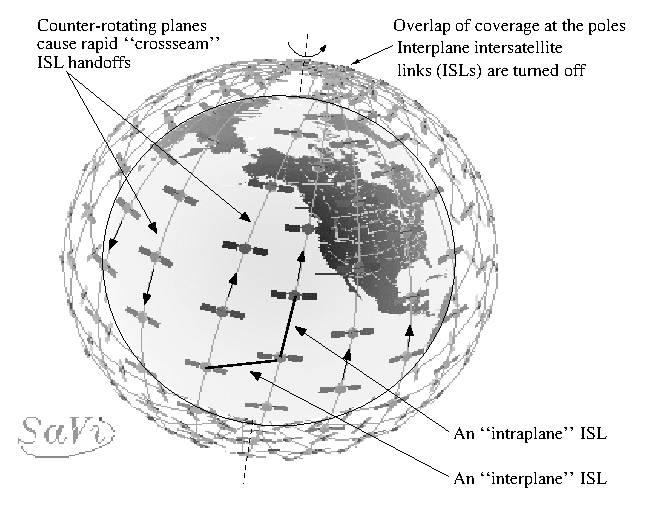
\includegraphics{sat-constellation}}
    \caption{Example of a polar-orbiting LEO constellation.  This figure
was generated using the SaVi software package from the geometry center at the
University of Minnesota.}
    \label{fig:constellation}
\end{figure}

Polar orbiting satellite systems, such as Iridium and the proposed Teledesic 
system, can
be modelled in \ns.   In particular, the simulator supports the specification
of satellites that orbit in purely circular planes, for which the neighboring 
planes are co-rotating.
There are other non-geostationary constellation configurations  
possible (e.g., Walker constellations)-- the interested user may develop new
constellation classes to simulate these other constellation types.  In
particular, this would mainly require defining new intersatellite link 
handoff procedures.

The following are the parameters of satellite constellations that can currently
be simulated:
\begin{itemize}
        \item {\bf Basic constellation definition} Includes satellite altitude,
number of satellites, number of planes, number of satellites per plane.
        \item {\bf Orbits} Orbit inclination can range continuously
from 0 to 180 degrees (inclination greater than 90 degrees corresponds to
retrograde orbits).  Orbit eccentricity is not modeled.  Nodal precession is 
not modeled.  Intersatellite spacing within a given plane is fixed.  Relative
phasing between planes is fixed (although some systems may not control phasing
between planes).
        \item {\bf Intersatellite (ISL) links} For polar orbiting 
constellations,
intraplane, interplane, and crossseam ISLs can be defined.  Intraplane ISLs
exist between satellites in the same plane and are never deactivated or 
handed off.  Interplane ISLs exist between satellites of neighboring 
co-rotating planes.  These links are deactivated near the poles (above
the ``ISL latitude threshold'' in the table) because the antenna pointing 
mechanism cannot track these links in the polar regions.  Like intraplane ISLs,
interplane ISLs are never handed off.  Crossseam ISLs may exist in a 
constellation between satellites in counter-rotating planes (where the 
planes form a so-called ``seam'' in the topology).   GEO ISLs can also be
defined for constellations of geostationary satellites.
        \item {\bf Ground to satellite (GSL) links}  Multiple terminals
can be connected to a single GSL satellite channel.  GSL links for GEO 
satellites are static, while GSL links for LEO channels are periodically 
handed off as described below.  
        \item {\bf Elevation mask} The elevation angle above which a GSL 
link can be operational.  Currently, if the (LEO) satellite serving a terminal
drops below the elevation mask, the terminal searches for a new satellite
above the elevation mask.  Satellite terminals check for handoff opportunities
according to a timeout interval specified by the user.  Each terminal
initiates handoffs asynchronously; it would be possible also to define
a system in which each handoff occurs synchronously in the system.
\end{itemize}

The following table lists parameters used for example simulation scripts
of the Iridium\footnote{Aside
from the link bandwidths (Iridium is a narrowband system only), these
parameters are very close to what a broadband version of the Iridium system
might look like.}  and Teledesic\footnote{These Teledesic constellation 
parameters are subject to change; 
thanks to Marie-Jose Montpetit of Teledesic for providing
tentative parameters as of January 1999.  The link bandwidths are not
necessarily accurate.} systems.

\begin{table}[h]
\begin{center}
{\tt
\begin{tabular}{|c||c|c|}\hline
& {\bf Iridium} & {\bf Teledesic}\\\hline\hline
{\bf Altitude} & \rm 780 km& \rm 1375 km\\\hline
{\bf Planes} & \rm 6& \rm 12\\\hline
{\bf Satellites per plane} & \rm 11 & \rm 24\\\hline
{\bf Inclination (deg)} & \rm 86.4 & \rm 84.7\\\hline
{\bf Interplane separation (deg)} & \rm 31.6 & \rm 15\\\hline
{\bf Seam separation (deg)} & \rm 22 & \rm 15\\\hline
{\bf Elevation mask (deg)} & \rm 8.2 & \rm 40\\\hline
{\bf Intraplane phasing} & \rm yes & \rm yes\\\hline
{\bf Interplane phasing} & \rm yes & \rm no\\\hline
{\bf ISLs per satellite} & \rm 4  & \rm 8\\\hline
{\bf ISL bandwidth} & \rm 25 Mb/s  & \rm 155 Mb/s\\\hline
{\bf Up/downlink bandwidth} & \rm 1.5 Mb/s  & \rm 1.5 Mb/s\\\hline
{\bf Cross-seam ISLs} & \rm no & \rm yes\\\hline
{\bf ISL latitude threshold (deg)} & \rm 60 & \rm 60\\\hline
\end{tabular}
}
\end{center}
\caption{Simulation parameters used for modeling a broadband version of
the Iridium system and the proposed 288-satellite Teledesic system.
Both systems are examples of polar orbiting constellations.
}
\end{table}
\clearpage
%%%%%%%%%%%%%%%%%%%%%%%%%%%%%%%%%%%%%%%%%%%%%%%%%%%%%%%%%%%%%%%%%%%%%%%%%%
%%%%%%%%%%%%%%%%%%%%%%%%%%%%%%%%%%%%%%%%%%%%%%%%%%%%%%%%%%%%%%%%%%%%%%%%%%

\section{Using the satellite extensions}
\label{sec:satellite/usage}

\begin{figure}
    \centerline{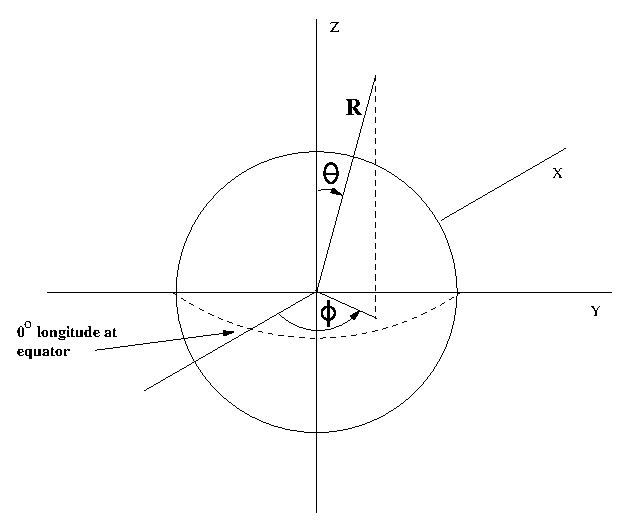
\includegraphics{sat-spherical}}
    \caption{Spherical coordinate system used by satellite nodes}
    \label{fig:spherical}
\end{figure}

%%%%%%%%%%%%%%%%%%%%%%%%%%%%%%%%%%%%%%%%%%%%%%%%%%%%%%%%%%%%%%%%%%%%%%%%%%

\subsection{Nodes and node positions}
\label{sec:satellite/usage/nodes}

There are two basic kinds of satellite nodes:  {\em geostationary}  
and {\em non-geostationary} satellite nodes.  In addition, {\em terminal} nodes
can be placed on the Earth's surface.  As is explained later in 
Section \ref{sec:satellite/implementation},
each of these three different types of nodes is actually implemented with 
the same \code{class SatNode} object, but with different position,
handoff manager,  and link objects attached.  
The position object keeps track of the satellite node's location 
in the coordinate system as a function of the elapsed simulation time.
This position information is used to determine link propagation delays and
appropriate times for link handoffs. 

Figure \ref{fig:spherical} illustrates the spherical coordinate system,
and the corresponding Cartesian coordinate system.
The coordinate system is centered at the 
Earth's center, and the $z$ axis coincides with the Earth's axis of rotation.  
$(R,\theta,\phi) = (6378 km, 90^o, 0^o)$ corresponds to $0^o$ longitude 
(prime meridian) on the equator.

Specifically, there is one class of satellite node \code{Class Node/SatNode},
to which one of three types of \code{Position} objects may be attached.  
Each \code{SatNode} and \code{Position} object is a split OTcl/C++ object,
but most of the code resides in C++.  The following types of position objects 
exist: 
\begin{itemize}
\item \code{Position/Sat/Term} A terminal is specified by its latitude and
longitude.  Latitude ranges from $[-90, 90]$ and longitude ranges from
$[-180, 180]$, with negative values corresponding to south and west, 
respectively.  As simulation time evolves, the terminals move along
with the Earth's surface.  The  Simulator instproc \code{satnode} can be used 
to create a terminal with an attached position object as follows:
\begin{program}
$ns satnode terminal $lat $lon
\end{program}
\item \code{Position/Sat/Geo} A geostationary satellite is specified by its 
longitude above the equator.  As simulation time evolves, the geostationary
satellite moves through the coordinate system with the same orbital period
as that of the Earth's rotation.  The longitude ranges from $[-180,180]$
degrees.  The Simulator instproc \code{satnode} can be 
used to create a geostationary satellite with an attached position object as 
follows:
\begin{program}
$ns satnode geo $lon
\end{program}
\item \code{Position/Sat/Polar} A polar orbiting satellite has a purely
circular orbit along a fixed plane in the coordinate system; the Earth
rotates underneath this orbital plane, so there is both an east-west and
a north-south component to the track of a polar satellite's footprint on
the Earth's surface.  Strictly speaking, the polar position object can
be used to model the movement of any circular orbit in a fixed plane;  
we use the term ``polar'' here because we later use such satellites to model 
polar-orbiting constellations.

Satellite orbits are usually specified by six parameters:  {\em altitude},
{\em semi-major axis}, {\em eccentricity}, 
{\em right ascension of ascending node}, {\em inclination}, and
{\em time of perigee passage}.  The polar orbiting satellites in \ns~have
purely circular orbits, so we simplify the specification of the orbits to
include only three parameters: {\em altitude}, {\em inclination}, and
{\em longitude}, with a fourth parameter {\em alpha} specifying initial 
position of the satellite in the orbit, as described below.
{\bf Altitude} is specified in kilometers above the Earth's surface, and 
{\bf inclination} can range from $[0,180]$ degrees, with $90$ corresponding
to pure polar orbits and angles greater than $90$ degrees corresponding
to ``retrograde'' orbits.  The {\em ascending node} refers to the point
where the footprint of the satellite orbital track crosses the equator 
moving from south to north.  In this simulation model, the parameter 
{\bf longitude of ascending node} specifies the earth-centric longitude at 
which the satellite's nadir point crosses the equator moving south
to north.\footnote{Traditionally, the ``right ascension'' of the ascending
node is specified for satellite orbits-- the right ascension corresponds to the 
{\em celestial} longitude.  In our case, we do not care about the
orientation in a celestial coordinate system, so we specify the earth-centric
longitude instead.} {\em Longitude of ascending node} can range from 
$[-180,180]$ degrees.  The fourth parameter,
{\bf alpha}, specifies the initial position of the satellite along this
orbit, starting from the ascending node.  
For example, an {\em alpha} of $180$ degrees indicates that the
satellite is initially above the equator moving from north to south.
{\em Alpha} can range from $[0,360]$ degrees.
Finally, a fifth parameter, {\bf plane}, is specified when creating
polar satellite nodes-- all satellites in the same plane are given the
same plane index.
The Simulator instproc \code{satnode} can be 
used to create a polar satellite with an attached position object as 
follows:
\begin{program}
$ns satnode polar $alt $inc $lon $alpha $plane
\end{program}

\end{itemize}

%%%%%%%%%%%%%%%%%%%%%%%%%%%%%%%%%%%%%%%%%%%%%%%%%%%%%%%%%%%%%%%%%%%%%%%%%%

\subsection{Satellite links}
\label{sec:satellite/usage/links}

\begin{figure}
    \centerline{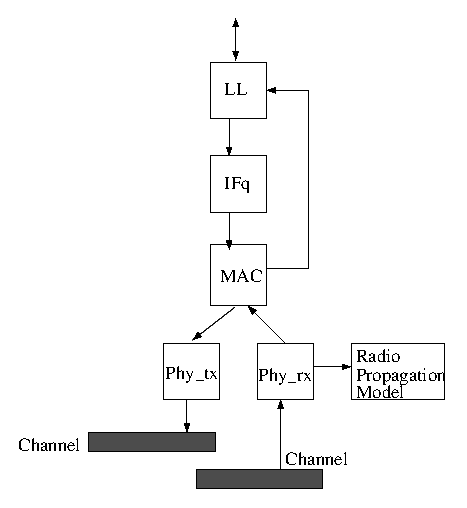
\includegraphics{sat-stack-basic}}
    \caption{Main components of a satellite network interface}
    \label{fig:sat-stack-basic}
\end{figure}

Satellite links resemble wireless links, which are described in Chapter
\ref{chap:mobility}.  Each satellite
node has one or more satellite network interface stacks, to which
channels are connected to the physical layer object in the stack.  Figure
\ref{fig:sat-stack-basic} illustrates the major components.  Satellite
links differ from \ns~wireless links in two major respects:  i) the
transmit and receive interfaces must be connected to different channels,
and ii) there is no ARP implementation.  Currently, the {\em
Radio Propagation Model} is a placeholder for users to add more detailed
error models if so desired; the current code does not use a propagation
model.

Network interfaces can be added with the following instproc of
\code{Class Node/SatNode}:
\begin{program}
$node add-interface $type $ll $qtype $qlim $mac $mac_bw $phy
\end{program}
The \code{add-interface} instproc returns an index value that can be used
to access the network interface stack later in the simulation.  By convention,
the first interface created on a node is attached to the uplink and downlink
channels of a satellite or terminal.  The
following parameters must be provided:

\begin{itemize} 
	\item {\bf type}:~~The following link types can be indicated:  
\code{geo} or 
\code{polar} for links from a terminal to a geo or polar satellite, 
respectively, \code{gsl} and \code{gsl-repeater} for links from a satellite
to a terminal, and \code{intraplane}, \code{interplane}, and \code{crossseam}
ISLs.  The type field is used internally in the simulator to identify the
different types of links, but structurally they are all very similar.
	\item {\bf ll}:~~The link layer type (\code{class LL/Sat} is currently
the only one defined).  
	\item {\bf qtype}:~~The queue type (e.g., \code{class Queue/DropTail}).
Any queue type may be used-- however, if additional parameters beyond the
length of the queue are needed, then this instproc may need to be modified
to include more arguments.
	\item {\bf qlim}:~~The length of the interface queue, in packets.
	\item {\bf mac}:~~The MAC type.  Currently, two types are defined:
\code{class Mac/Sat}-- a basic MAC for links with only one receiver (i.e.,
it does not do collision detection), and
\code{Class Mac/Sat/UnslottedAloha}-- an implementation of unslotted Aloha.
	\item {\bf mac\_bw}:~~The bandwidth of the link is set by this 
parameter, which controls the transmission time how fast the MAC sends. The
packet size used to calculate the transmission time is the sum of the
values \code{size()} in the common packet header and \code{LINK_HDRSIZE},
which is the size of any link layer headers.  The default value for
\code{LINK_HDRSIZE} is 16 bytes (settable in \code{satlink.h}).
The transmission time is encoded in the packet header for use at the
receive MAC (to simulate waiting for a whole packet to arrive).  
	\item {\bf phy}:~~The physical layer-- currently two Phys 
(\code{Class Phy/Sat} and \code{Class Phy/Repeater}) are defined.  
The class \code{Phy/Sat} just pass the information up and down the stack--
as in the wireless code described in Chapter \ref{chap:mobility}, 
a radio propagation model could be attached at this point.  The class
\code{Phy/Repeater} pipes any packets received on a receive interface
straight through to a transmit interface.
\end{itemize}

An ISL can be added between two nodes using the following instproc:
\begin{program}
$ns add-isl $ltype $node1 $node2 $bw $qtype $qlim
\end{program}
This creates two channels (of type \code{Channel/Sat}), and appropriate
network interfaces on both nodes, and attaches the channels to the 
network interfaces.  The bandwidth of the link is
set to \code{bw}.  The linktype (\code{ltype})
must be specified as either \code{intraplane}, \code{interplane}, or 
\code{crossseam}.


A GSL involves adding network interfaces and a channel on board the
satellite (this is typically done using the wrapper methods described
in the next paragraph), and then defining the correct interfaces on
the terrestrial node and attaching them to the satellite link, as 
follows:
\begin{program}
$node add-gsl $type $ll $qtype $qlim $mac $bw_up $phy \bs
   [$node_satellite set downlink_] [$node_satellite set uplink_]
\end{program}
Here, the \code{type} must be either \code{geo} or \code{polar}, 
and we make use
of the \code{downlink_} and \code{uplink_} instvars of the satellite;
therefore, the satellite's uplink and downlink must be created before
this instproc is called.

Finally, the following wrapper methods can be used to create nodes of a 
given type and, in the case of satellite nodes, give them an uplink and
downlink interface as well as create and attach an uplink and downlink
channel: 
\begin{program}
$ns satnode-terminal $latitude $longitude
$ns satnode-polar $alt $inc $lon $alpha $plane $linkargs $chan
$ns satnode-geo $longitude $linkargs $chan
$ns satnode-geo-repeater $longitude $chan
\end{program}
where \code{linkargs} is a list of link argument options for the 
network interfaces (i.e., \code{$ll $qtype $qlim $mac $mac_bw $phy}). 


%%%%%%%%%%%%%%%%%%%%%%%%%%%%%%%%%%%%%%%%%%%%%%%%%%%%%%%%%%%%%%%%%%%%%%%%%%

\subsection{Handoffs }
\label{sec:satellite/usage/handoffs}

Satellite handoff modelling is a key component of LEO satellite network 
simulations.  It is difficult to predict exactly how handoffs will occur
in future LEO systems because the subject is not well treated in the
literature.  In these satellite extensions, we establish certain criteria for 
handoffs, and allow nodes to independently monitor for situations that 
require a handoff.  An alternative would be to have all handoff events
synchronized across the entire simulation-- it would not be difficult to 
change the simulator to work in such a manner.

There are no link handoffs involving geostationary satellites, but there 
are two types of links to polar orbiting satellites
that must be handed off:  GSLs to polar satellites, and crossseam ISLs.  
A third type of link, interplane ISLs, are not handed off but are deactivated
at high latitudes as we describe below.

Each terminal connected to a polar orbiting satellite runs a timer that,
upon expiry, causes the \code{HandoffManager} to check whether the current 
satellite has fallen below the
elevation mask of the terminal.  If so, the handoff manager detaches the
terminal from that satellite's up and down links, and searches
through the linked list of satellite nodes for another possible satellite.
First, the ``next'' satellite in the current orbital plane is checked-- a 
pointer to this satellite is stored in the Position object of each
polar satellite node and is set during simulation configuration using
the \code{Node/SatNode} instproc ``\code{$node set_next $next_node}.''
If the next satellite is not suitable, the handoff manager searches
through the remaining satellites.  If it finds a suitable polar
satelite, it connects its network interfaces to that satellite's uplink and 
downlink channels, and restarts the handoff timer.  If it does not find 
a suitable
satellite, it restarts the timer and tries again later.  If any link
changes occur, the routing agent is notified.

The elevation mask and handoff timer interval are settable via OTcl: 
\begin{program}
HandoffManager/Term set elevation_mask_ 10; # degrees
HandoffManager/Term set term_handoff_int_ 10; # seconds
\end{program}
In addition, handoffs may be randomized to avoid phase effects by setting
the following variable:
\begin{program}
HandoffManager set handoff_randomization_ 0; # 0 is false, 1 is true 
\end{program}
If \code{handoff_randomization_} is true, then the next handoff interval
is a random variate picked from a uniform distribution across
$(0.5 * term\_handoff\_int\_, 1.5 * term\_handoff\_int\_)$.  

Crossseam ISLs are the only type of ISLs that are handed off.  The criteria
for handing off a crossseam ISL is whether or not there exists a satellite
in the neighboring plane that is closer to the given satellite than the
one to which it is currently connected.  Again, a handoff timer running
within the handoff manager on the polar satellite determines when the
constellation is checked for handoff opportunities.  Crossseam ISL
handoffs are
initiated by satellites in the lower-numbered plane of the two.  It is
therefore possible for a transient condition to arise in which a polar
satellite has two crossseam ISLs (to different satellites).  The
satellite handoff interval is again settable from OTcl and may also be
randomized:
\begin{program}
HandoffManager/Sat set sat_handoff_int_ 10; # seconds
\end{program}

Interplane and crossseam ISLs are deactivated near the poles, because 
the pointing requirements for the links are too severe as the satellite
draw close to one another.  Shutdown of these links is governed by a parameter:
\begin{program}
HandoffManager/Sat set latitude_threshold_ 70; # degrees 
\end{program}
The values for this parameter in the example scripts are speculative;
the exact value is dependent upon the satellite hardware.  The handoff
manager checks the latitude of itself and its peer satellite upon a handoff
timeout; if either or both of the satellites is above 
\code{latitude_threshold_} degrees latitude (north or south), the link
is deactivated until both satellites drop below this threshold.

Finally, if crossseam ISLs exist, there are certain situations in which
the satellites draw too close to one another in the mid-latitudes (if
the orbits are not close to being pure polar orbits).  We check for
the occurence of this orbital overlap with the following parameter:
\begin{program}
HandoffManager/Sat set longitude_threshold_ 10; # degrees 
\end{program}
Again, the values for this parameter in the example scripts are speculative.
If the two satellites are closer together in longitude than 
\code{longitude_threshold_} degrees, the link between them is deactivated.
This parameter is disabled (set to $0$) by default-- all defaults for
satellite-related bound variables can be found in \nsf{tcl/lib/ns-sat.tcl}.


%%%%%%%%%%%%%%%%%%%%%%%%%%%%%%%%%%%%%%%%%%%%%%%%%%%%%%%%%%%%%%%%%%%%%%%%%%

\subsection{Routing }
\label{sec:satellite/usage/routing}

The current status of routing is that it is incomplete.  Ideally, one should
be able to run all existing \ns~routing protocols over satellite links.  
However,
many of the existing routing protocols implemented in OTcl require that
the conventional \ns~links be used.  The \ns~developers are working to
remedy this situation so that existing routing implementations are 
independent of the underlying link objects.

With that being said, the current routing implementation is similar to
Session routing described in Chapter \ref{chap:unicast}, except that it
is implemented entirely in C++.   Upon each topology change, a centralized
routing genie determines the global network topology, computes new routes
for all nodes, and uses the routes to build
a forwarding table on each node.  Currently,
the slot table is kept by a routing agent on each node, and packets 
not destined for agents on the node are sent by default to this routing 
agent.  For each destination for which the node has a route, the forwarding
table contains a pointer to the head of the corresponding outgoing link.
As noted in Chapter \ref{chap:unicast}, the user is cautioned that this type 
of centralized routing can lead to minor causality violations.

The routing genie is a \code{class SatRouteObject} and is created and
invoked with the following OTcl commands:
\begin{program}
set satrouteobject_ [new SatRouteObject]
$satrouteobject_ compute_routes
\end{program}
where the call to \code{compute_routes} is performed after all of the
links and nodes in the simulator have been instantiated.
Like the \code{Scheduler}, there is one instance of a SatRouteObject in the
simulation, and it is accessed by means of an instance variable in C++.
For example, the call to recompute routes after a topology change is:
\begin{program}
SatRouteObject::instance().recompute();
\end{program}

Despite the current use of centralized routing, the design of having
a routing agent on each node was mainly done with distributed routing 
in mind.  Routing packets can be sent to port 255 of each node.  The key
to distributed routing working correctly is for the routing agent to
be able to 
determine from which link a packet arrived.  This is accomplished by the
inclusion of a \code{class NetworkInterface} object in each link, which
uniquely labels the link on which the packet arrived.  A helper function
\code{NsObject* intf_to_target(int label)} can be used to return the head 
of the
link corresponding to a given label.  The use of routing agents parallels
that of the mobility extensions, and the interested reader can turn to
those examples to see how to implement distributed routing protocols in
this framework.

The shortest-path route computations use the current propagation delay of
a link as the cost metric.  It is possible to compute routes using only
the hop count and not the propagation delays; in order to do so, set
the following default variable to "false":
\begin{program}
SatRouteObject set metric_delay_ "true"
\end{program}

Finally, for very large topologies (such as the Teledesic example), the 
centralized routing code will produce a very slow runtime because it executes
an all-pairs shortest path algorithm upon each topology change even if
there is no data currently being sent.  To speed up simulations in which
there is not much data transfer but there are lots of satellites and
ISLs, one can disable {\em handoff-driven} and enable {\em data-driven} 
route computations.  With data-driven computations, routes are computed
only when there is a packet to send, and furthermore, a single-source
shortest-path algorithm (only for the node with a packet to send) is 
executed instead of an all-pairs shortest path algorithm.  The following
OTcl variable can configure this option (which is set to "false" by
default):
\begin{program}
SatRouteObject set data_driven_computation_ "false"
\end{program}


%%%%%%%%%%%%%%%%%%%%%%%%%%%%%%%%%%%%%%%%%%%%%%%%%%%%%%%%%%%%%%%%%%%%%%%%%%

\subsection{Trace support}
\label{sec:satellite/usage/trace}

Tracefiles using satellite nodes and links are very similar to conventional
\ns~tracing described in Chapter \ref{chap:trace}.  Special SatTrace objects
(\code{class SatTrace} derives from \code{class Trace}) are used
to log the geographic latitude and longitude of the node logging the trace
(in the case of a satellite node, the latitude and longitude correspond
to the nadir point of the satellite).

For example, a packet on a link from node 66 to node 26 might normally be
logged as:  
\begin{program}
+ 1.0000 66 26 cbr 210 ------- 0 66.0 67.0 0 0 
\end{program}
but in the satellite simulation, the position information is appended:
\begin{program}
+ 1.0000 66 26 cbr 210 ------- 0 66.0 67.0 0 0 37.90 -122.30 48.90 -120.94
\end{program}
In this case, node 66 is at latitude 37.90 degrees, longitude -122.30
degrees, while node 26 is a LEO satellite whose subsatellite
point is at 48.90 degrees latitude, -120.94 degrees longitude (negative
latitude corresponds to south, while negative longitude corresponds to
west).

One addition is the \code{Class Trace/Sat/Error}, which traces any packets
that are errored by an error model.  The error trace logs packets dropped
due to errors as follows, for example:  
\begin{program}
e 1.2404 12 13 cbr 210 ------- 0 12.0 13.0 0 0 -0.00 10.20 -0.00 -10.00
\end{program}

To enable tracing of all satellite links in the simulator, use the following
commands {\em before} instantiating nodes and links:
\begin{program}
set f [open out.tr w]
$ns trace-all $f
\end{program}
Then use the following line after all node and link creation (and all
error model insertion, if any) to enable tracing of all satellite links:
\begin{program}
$ns trace-all-satlinks $f
\end{program}
Specifically, this will put tracing around the link layer queues in all
satellite links, and will put a receive trace between the mac and the
link layer for received packets.  To enable tracing only on a specific
link on a specific node, one may use the command:
\begin{program}
$node trace-inlink-queue $f $i
$node trace-outlink-queue $f $i
\end{program}
where $i$ is the index of the interface to be traced.  

The implementations of the satellite trace objects can be found in 
\nsf{tcl/lib/ns-sat.tcl} and \nsf{sattrace.\{cc,h\}}.

%%%%%%%%%%%%%%%%%%%%%%%%%%%%%%%%%%%%%%%%%%%%%%%%%%%%%%%%%%%%%%%%%%%%%%%%%%

\subsection{Error models}
\label{sec:satellite/usage/error}

\ns~error models are described in Chapter \ref{chap:error_model}.  These
error models can be set to cause packets to be errored according to various
probability distributions.  These error models are simple and don't 
necessarily correspond to what would be experienced on an actual satellite
channel (particularly a LEO channel).  Users are 
free to define more sophisticated error models that more closely match a 
particular satellite environment.

The following code provides an example of how to add an error model to a
link:
\begin{program}
set em_ [new ErrorModel]
$em_ unit pkt
$em_ set rate_ 0.02
$em_ ranvar [new RandomVariable/Uniform]
$node interface-errormodel $em_ 
\end{program}
This will add an error model to the receive path of the first interface
created on node \code{$node} (specifically, between the MAC and link layer)--
this first interface generally corresponds to the uplink and downlink
interface for a satellite or a terminal (if only one uplink and/or downlink
exists).
To add the error model to a different stack (indexed by $i$), use the 
following code:
\begin{program}
$node interface-errormodel $em_ $i 
\end{program}


%%%%%%%%%%%%%%%%%%%%%%%%%%%%%%%%%%%%%%%%%%%%%%%%%%%%%%%%%%%%%%%%%%%%%%%%%%

\subsection{Other configuration options}
\label{sec:satellite/usage/other}

Given an initial configuration of satellites specified for time $0$, 
it is possible to start the 
satellite configuration from any arbitrary point in time through the use of the
\code{time_advance_} parameter (this is really only useful for LEO
simulations). During the simulation run, this will set the position of 
the object to the position at time
\code{Scheduler::instance().clock + time_advance_} seconds.
\begin{program}
Position/Sat set time_advance_ 0; # seconds          
\end{program}


%%%%%%%%%%%%%%%%%%%%%%%%%%%%%%%%%%%%%%%%%%%%%%%%%%%%%%%%%%%%%%%%%%%%%%%%%%

\subsection{\nam~~support}
\label{sec:satellite/usage/nam}
\nam~~is not currently supported.  Addition of \nam~~ for GEO satellite
topologies is an active work item.  \nam~~ support for LEO constellations is
not planned (interested users are encouraged to develop this component).

%%%%%%%%%%%%%%%%%%%%%%%%%%%%%%%%%%%%%%%%%%%%%%%%%%%%%%%%%%%%%%%%%%%%%%%%%%

\subsection{Integration with other modules}
\label{sec:satellite/usage/integration}
Currenty, these satellite extensions do not interoperate with the wireless
code, mobile-IP code, and OTcl routing protocols (in particular, multicast).
This is an active work item for the \ns~developers and more support along
these lines will be added later.

%%%%%%%%%%%%%%%%%%%%%%%%%%%%%%%%%%%%%%%%%%%%%%%%%%%%%%%%%%%%%%%%%%%%%%%%%%

\subsection{Example scripts}
\label{sec:satellite/usage/example}

Example scripts can be found in the \nsf{tcl/ex} directory, including:
\begin{itemize}
\item \code{sat-mixed.tcl}  A simulation with a mixture of polar and
geostationary satellites.
\item \code{sat-repeater.tcl}  Demonstrates the use of a simple bent-pipe
geostationary satellite, and also error models.
\item \code{sat-aloha.tcl}  Simulates one hundred terminals in a mesh-VSAT
configuration using an unslotted Aloha MAC protocol 
with a ``bent-pipe'' geostationary satellite.  Terminals listen to their
own transmissions (after a delay), and if they do not successfully receive
their own packet within a timeout interval, they perform exponential 
backoff and then retransmit the packet. 
\item \code{sat-iridium.tcl}  Simulates a broadband LEO constellation with
parameters similar to that of the Iridium constellation (with supporting
scripts \code{sat-iridium-links.tcl}, \code{sat-iridium-linkswithcross.tcl}, 
and \code{sat-iridium-nodes.tcl}).
\item \code{sat-teledesic.tcl}  Simulates a broadband LEO constellation with
parameters similar to those proposed for the 288 satellite Teledesic
constellation (with supporting scripts \code{sat-teledesic-links.tcl} and 
\code{sat-teledesic-nodes.tcl}).
\end{itemize}
In addition, there is a test suite script that tries to exercise a lot
of features simultaneously, it can be found at \nsf{tcl/test/test-suite-sat.tcl}.

%%%%%%%%%%%%%%%%%%%%%%%%%%%%%%%%%%%%%%%%%%%%%%%%%%%%%%%%%%%%%%%%%%%%%%%%%%
%%%%%%%%%%%%%%%%%%%%%%%%%%%%%%%%%%%%%%%%%%%%%%%%%%%%%%%%%%%%%%%%%%%%%%%%%%

\section{Implementation}
\label{sec:satellite/implementation}

The code for the implementation of satellite extensions can be found
in \nsf{\{sat.h, sathandoff.\{cc,h\}, satlink.\{cc,h\}, satnode.\{cc,h\}, 
satposition.\{cc,h\}, satroute.\{cc,h\}, sattrace.\{cc,h\}\}}, and
\nsf{tcl/lib/ns-sat.tcl}.  Almost all of the mechanism is implemented
in C++.

In this section, we focus on some of the key components of the implementation;
namely, the use of linked lists, the node structure, and a detailed look
at the satellite link structure.

\subsection{Use of linked lists}
\label{sec:satellite/implementation/list}

\begin{figure}
    \centerline{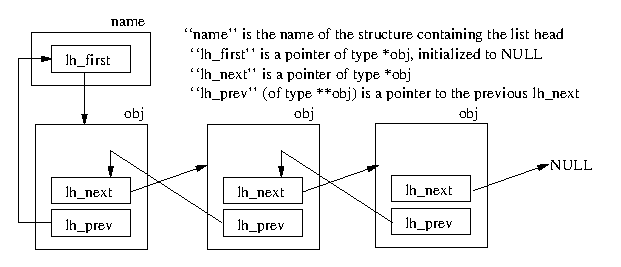
\includegraphics{linked-list}}
    \caption{Linked list implementation in \ns.}
    \label{fig:linked-list}
\end{figure}

There are a number of linked lists used heavily in the implementation:
\begin{itemize}

\item \code{class Node} maintains a (static) list of all objects of class
\code{Node} in the simulator.  The variable \code{Node::nodehead_} stores
the head of the list.  The linked list of nodes is used for centralized
routing, for finding satellites to hand off to, and for tracing.

\item \code{class Node} maintains a list of all (satellite) links on the
node.  Specifically, the list is a list of objects of class \code{LinkHead}. 
The variable \code{linklisthead_} stores the head of the list.  The
linked list of LinkHeads is used for checking whether or not to handoff
links, and to discover topology adjacencies.

\item \code{class Channel} maintains a list of all objects of class
\code{Phy} on the channel.  The head of the list is stored in the variable
\code{if_head_}.  This list is used to determine the set of interfaces on a
channel that should receive a copy of a packet.
\end{itemize}

Figure \ref{fig:linked-list} provides a schematic of how the linked list
is organized.  Each object in the list is linked through a ``LINK\_ENTRY''
that is a protected member of the class.  This entry contains a pointer
to the next item in the list and also a pointer to the address of the
previous ``next'' pointer in the preceding object.   Various macros
found in \nsf{list.h} can be used to manipulate the list; the 
implementation of linked-lists in \ns~is similar to the \code{queue} 
implementation found in some variants of BSD UNIX.

\subsection{Node structure}

\begin{figure}
    \centerline{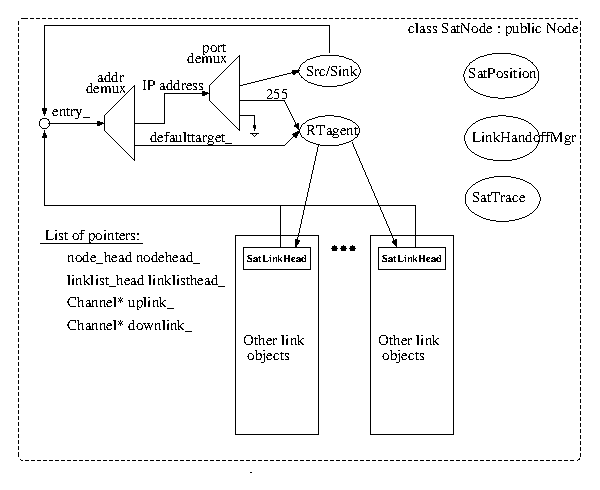
\includegraphics{sat-node}}
    \caption{Structure of \code{class SatNode}.}
    \label{fig:sat-node}
\end{figure}

Figure \ref{fig:sat-node} is a schematic of the main components of a
\code{SatNode}.  The structure bears resemblance to the \code{MobileNode}
in the wireless extensions, but there are several differences.  Like all
\ns~nodes, the SatNode has an ``entry'' point to a series of classifiers.
The address classifier contains a slot table for forwarding packets to 
foreign nodes, but since OTcl routing is not used, all packets not destined
for this node (and hence forwarded to the port classifier), are sent to
the default target, which points to a routing agent.  Packets destined
on the node for port 255 are classified as routing packets and are also
forwarded to the routing agent.

Each node contains one or more ``network stacks'' that include a generic
\code{SatLinkHead} at the entry point of the link.  The \code{SatLinkHead}
is intended to serve as an API to get at other objects in the link structure,
so it contains a number of pointers (although the API here has not been
finalized).  Packets leaving the network stack are sent to the node's
entry.  An important feature is that each packet leaving a network stack
has its \code{iface_} field in the common packet header coded with the
unique \code{NetworkInterface} index corresponding to the link.  This value
can be used to support distributed routing as described below.

The base class routing agent is \code{class SatRouteAgent}; it can be used 
in conjunction with centralized routing.  SatRouteAgents contain
a forwarding table that resolves a packet's address to a particular 
LinkHead target-- it is the job of the \code{SatRouteObject} to populate this
table correctly.  The SatRouteAgent populates certain fields in the header
and then sends the packet down to the approprate link.  To implement
a distributed routing protocol, a new SatRouteAgent could be defined-- this
would learn about topology by noting the interface index marked in each 
packet as it came up the stack-- a helper function in the node 
\code{intf_to_target()} allows it to resolve an index value to
a particular LinkHead. 

There are pointers to three additional objects in a SatNode.  First,
each SatNode contains a position object, discussed in the previous section.
Second, each SatNode contains a \code{LinkHandoffMgr} that monitors
for opportunities to hand links off and coordinates the handoffs.  Satellite
nodes and terminal nodes each have their specialized version of a 
LinkHandoffMgr.

Finally, a number of pointers to objects are contained in a SatNode.  We
discussed \code{linklisthead_} and \code{nodehead_} in the previous 
subsection.  The \code{uplink_} and \code{downlink_} pointers are
used for convenience under the assumption that, in most simulations,
a satellite or a terminal has only one uplink and downlink channel.

\subsection{Detailed look at satellite links}
\begin{figure}
    \centerline{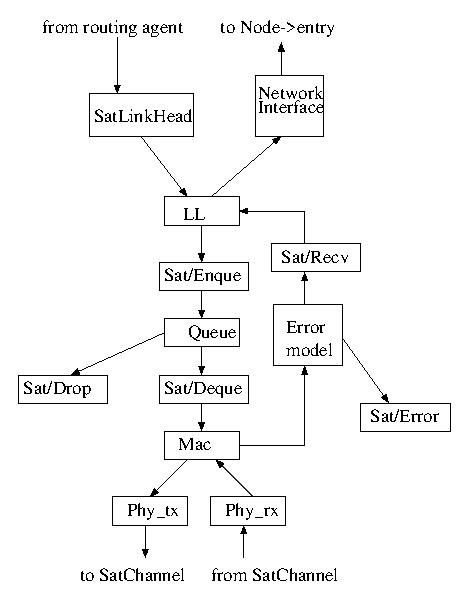
\includegraphics{sat-stack}}
    \caption{Detailed look at network interface stack.}
    \label{fig:sat-stack}
\end{figure}

Figure \ref{fig:sat-stack} provides a more detailed look at how satellite links
are composed.  In this section, we describe how packets move up and down
the stack, and the key things to note at each layer.  The file 
\nsf{tcl/lib/ns-sat.tcl} contains the various OTcl instprocs that assemble
links according to Figure \ref{fig:sat-stack}.  We describe the composite
structure herein as a ``network stack.''  Most of the code for the
various link components is in \nsf{satlink.\{cc,h\}}.

The entry point to a network stack is the \code{SatLinkHead} object.  The
SatLinkHead object derives from \code{Class LinkHead}; the aim of link
head objects is to provide a uniform API for all network stacks.
\footnote{In the author's opinion, all network stacks in \ns~ should 
eventually have a LinkHead object at the front-- the class SatLinkHead 
would then disappear.}  The SatLinkHead object contains pointers to
the LL, Queue, MAC, Error model, and both Phy objects.  The SatLinkHead
object can also be queried as to what type of network stack it is-- e.g.,
GSL, interplane ISL, crossseam ISL, etc..  Valid codes for the \code{type_} 
field are currently found in \nsf{sat.h}.  Finally, the SatLinkHead
stores a boolean variable \code{linkup_} that indicates whether
the link to at least one other node on the channel is up.  The C++
implementation of SatLinkHead is found in \nsf{satlink.\{cc,h\}}.

Packets leaving a node pass through the SatLinkHead transparently to the 
\code{class SatLL} object.  The SatLL class derives from LL (link layer).
Link layer protocols (like ARQ protocols) can be defined here.  The current
SatLL assigns a MAC address to the packet.  Note that in the satellite case,
we do not use an Address Resolution Protocol (ARP); instead, we simply use
the MAC \code{index_} variable as its address, and we use a helper function
to find the MAC address of the corresponding interface of the next-hop node.  
Since \code{class LL} derives from \code{class LinkDelay}, the \code{delay_}
parameter of LinkDelay can be used to model any processing delay in the
link layer; by default this delay is zero.

The next object an outgoing packet encounters is the interface queue.  
However, if tracing is enabled, tracing elements may surround the
queue, as shown in Figure \ref{fig:sat-stack}.  This part of a satellite
link functions like a conventional \ns~ link.

The next layer down is the MAC layer.  The MAC layer draws packets from
the queue (or deque trace) object-- a handshaking between the MAC and the 
queue allows the MAC to draw packets out of the queue as it needs them.  The
transmission time of a packet is modelled in the MAC also-- the MAC computes
the transmission delay of the packet (based on the sum of the 
LINK\_HDRSIZE field defined in \code{satlink.h} and the \code{size} field 
in the common packet header), and does not call up for another packet until
the current one has been ``sent'' to the next layer down.  Therefore, it
is important to set the bandwidth of the link correctly at this layer.
For convenience, the transmit time is encoded in the \code{mac} header; this
information can be used at the receiving MAC to calculate how long it must
wait to detect a collision on a packet, for example.

Next, the packet is sent to a transmitting interface (Phy\_tx) of class 
\code{SatPhy}.  This
object just sends the packet to the attached channel.  We noted earlier
in this chapter that all interfaces attached to a channel are part of the
linked list for that channel.  This is not true for transmit interfaces,
however.  Only receive interfaces attached to a channel comprise this linked
list, since only receive interfaces should get a copy of transmitted packets.
The use of separate transmit and receive interfaces mirrors the real world
where full-duplex satellite links are made up of RF channels at different
frequencies.

The outgoing packet is next sent to a \code{SatChannel}, which copies the
packet to every receiving interface (of class \code{SatPhy}) on the channel. 
The Phy\_rx sends the packet to the MAC layer.  At the MAC layer, the packet
is held for the duration of its transmission time (and any appropriate
collision detection is performed if the MAC, such as the Aloha MAC,
supports it).  If the packet is determined to have arrived safely at the MAC,
it next passes to an \code{ErrorModel} object, if it exists.  If not, the
packet moves through any receive tracing objects to the \code{SatLL}
object.  The SatLL object passes the packet up after a processing delay
(again, by default, the value for \code{delay_} is zero).

The final object that a received packet passes through is an object of
\code{class NetworkInterface}.  This object stamps the \code{iface_} field
in the common header with the network stack's unique index value.  This
is used to keep track of which network stack a packet arrived on.  The
packet then goes to the \code{entry} of the SatNode (usually, an address
classifier).  

Finally, ``geo-repeater'' satellites exist, as described earlier in this
chapter.  Geo-repeater network stacks are very simple-- they only contain
a Phy\_tx and a Phy\_rx of \code{class RepeaterPhy}, and a SatLinkHead.  
Packets received by a Phy\_rx are sent to the Phy\_tx without delay.  The
geo-repeater satellite is a degenerate satellite node, in that it does not
contain things like tracing elements, handoff managers, routing agents, or 
any other link interfaces other than repeater interfaces.

\endinput




%----------------------------------------------------------------------------
\chapter{Radio Propagation Models}
\label{chap:propagation}

This chapter describes the radio propagation models implemented in \ns.
These models are used to predict the received signal power of
each packet. At the physical layer of each wireless node, there is a receiving
threshold. When a packet is received, if its signal power is below the receiving
threshold, it is marked as error and dropped by the MAC layer.

Up to now there are three propagation models in \ns, which are the free
space model\footnote{Based on the code contributed to \ns~from the CMU Monarch
project.}, two-ray ground reflection model\footnote{Contributed to \ns~from the
CMU Monarch project.} and the shadowing model\footnote{Implemented in \ns~by
Wei Ye at USC/ISI}. Their implementation can be found in \nsf{propagation.\{cc,h\}},
\nsf{tworayground.\{cc,h\}} and \nsf{shadowing.\{cc,h\}}. This documentation
reflects the APIs in ns-2.1b7.

%----------------------------------------------------------------------------
\section{Free space model}
\label{sec:freespace}

The free space propagation model assumes the ideal propagation condition
that there is only one clear line-of-sight path between the transmitter and
receiver. H. T. Friis presented the following equation to
calculate the received signal power in free space at distance $d$ from the
transmitter \cite{Friis46}.

\begin{equation}
  P_r (d) = \frac{P_t G_t G_r \lambda^2}{(4\pi)^2 d^2 L}
  \label{eqn:freespace}
\end{equation}

where $P_t$ is the transmitted signal power. $G_t$ and $G_r$ are the antenna
gains of the transmitter and the receiver respectively. $L (L\ge1)$ is the
system loss, and $\lambda$ is the wavelength. It is common to select
$G_t = G_r = 1$ and $L = 1$ in \ns~ simulations.

The free space model basically represents the communication range as a circle
around the transmitter. If a receiver is within the circle, it receives all
packets. Otherwise, it loses all packets

The OTcl interface for utilizing a propagation model is the \code{node-config}
command. One way to use it here is

\begin{program}
$ns_ node-config -propType Propagation/FreeSpace
\end{program}

Another way is

\begin{program}
set prop [new Propagation/FreeSpace]
$ns_ node-config -propInstance $prop
\end{program}

%----------------------------------------------------------------------------
\section{Two-ray ground reflection model}
\label{sec:tworay}

A single line-of-sight path between two mobile nodes is seldom the only means
of propation. The two-ray ground reflection model considers both the direct
path and a ground reflection path. It is shown \cite{Rappaport96} that this
model gives more accurate prediction at a long distance than the free space
model. The received power at distance $d$ is predicted by

\begin{equation}
  P_r (d) = \frac{P_t G_t G_r {h_t}^2 {h_r}^2}{d^4 L}
  \label{eqn:tworay}
\end{equation}

where $h_t$ and $h_r$ are the heights of the transmit and receive antennas
respectively. Note that the original equation in \cite{Rappaport96} assumes
$L = 1$. To be consistent with the free space model, $L$ is added here.

The above equation shows a faster power loss than Eqn. (\ref{eqn:freespace})
as distance increases. However, The two-ray model does not give a good result
for a short distance due to the oscillation caused by the constructive and
destructive combination of the two rays. Instead, the free space model is
still used when $d$ is small.

Therefore, a cross-over distance $d_c$ is calculated in this model. When
$d < d_c$, Eqn. (\ref{eqn:freespace}) is used. When $d > d_c$, Eqn.
(\ref{eqn:tworay}) is used. At the cross-over distance, Eqns. (\ref{eqn:freespace})
and (\ref{eqn:tworay}) give the same result. So $d_c$ can be calculated as

\begin{equation}
%  d_c = \frac{4\pi h_t h_r}{\lambda}
  d_c = \left( 4\pi h_t h_r \right) / \lambda
  \label{eqn:crossover}
\end{equation}

Similarly, the OTcl interface for utilizing the two-ray ground reflection model
is as follows.

\begin{program}
$ns_ node-config -propType Propagation/TwoRayGround
\end{program}

Alternatively, the user can use

\begin{program}
set prop [new Propagation/TwoRayGround]
$ns_ node-config -propInstance $prop
\end{program}


%----------------------------------------------------------------------------
\section{Shadowing model}
\label{sec:shadowing}

\subsection{Backgroud}

The free space model and the two-ray model predict the received power
as a deterministic function of distance. They both represent the communication
range as an ideal circle. In reality, the received power at certain distance
is a random variable due to multipath propagation effects, which is also
known as fading effects. In fact, the above two models predicts the mean
received power at distance $d$. A more general and widely-used model is
called the shadowing model~\cite{Rappaport96}.

The shadowing model consists of two parts. The first one is known as path
loss model, which also predicts the mean received power at distance $d$,
denoted by $\overline{P_r(d)}$. It uses a close-in distance $d_0$ as
a reference. $\overline{P_r(d)}$ is computed relative to $P_r(d_0)$
as follows.

\begin{equation}
  \frac{P_r(d_0)}{\overline{P_r(d)}} = {\left( \frac{d}{d_0} \right)}^\beta
  \label{eqn:pathloss}
\end{equation}

$\beta$ is called the path loss exponent, and is usually empirically
determined by field measurement. From Eqn. (\ref{eqn:freespace}) we
know that $\beta = 2$ for free space propagation. Table~\ref{tab:pathlossexp}
gives some typical values of $\beta$.
Larger values correspond to more obstructions and hence faster
decrease in average received power as distance becomes larger. $P_r(d_0)$
can be computed from Eqn. (\ref{eqn:freespace}).

\begin{table}
\begin{center}
  \centering \small
  \begin{tabular}{|l|l|c|}
  \hline \multicolumn{2}{|c|}{\bf{Environment}} & $\beta$ \\
  \hline Outdoor & Free space & 2 \\
  \cline{2 - 3}  & Shadowed urban area & 2.7 to 5 \\
  \hline In building & Line-of-sight & 1.6 to 1.8 \\
  \cline{2 - 3}  & Obstructed & 4 to 6 \\ \hline
  \end{tabular}
  \caption{Some typical values of path loss exponent $\beta$}
  \label{tab:pathlossexp}
\end{center}
\end{table}
\begin{table}
\begin{center}
  \centering \small
  \begin{tabular}{|l|c|}
  \hline \bf{Environment} & $\sigma_{dB}$ (dB) \\
  \hline Outdoor & 4 to 12 \\
  \hline Office, hard partition & 7 \\
  \hline Office, soft partition & 9.6 \\
  \hline Factory, line-of-sight & 3 to 6 \\
  \hline Factory, obstructed & 6.8 \\ \hline
  \end{tabular}
  \caption{Some typical values of shadowing deviation $\sigma_{dB}$}
  \label{tab:stddb}
\end{center}
\end{table}

The path loss is usually measured in dB. So from Eqn. (\ref{eqn:pathloss})
we have

\begin{equation}
  {\left[ \frac{\overline{P_r(d)}}{P_r(d_0)} \right]}_{dB} =
    -10 \beta \log \left( \frac{d}{d_0} \right)
  \label{eqn:pathlossdb}
\end{equation}

The second part of the shadowing model reflects the variation of the
received power at certain distance. It is a log-normal random variable,
that is, it is of Gaussian distribution if measured in dB. The overall
shadowing model is represented by

\begin{equation}
{\left[ \frac{P_r(d)}{P_r(d_0)} \right]}_{dB} =
    -10 \beta \log \left( \frac{d}{d_0} \right) + X_{dB}
  \label{eqn:shadowing}
\end{equation}

where $X_{dB}$ is a Gaussian random variable with zero mean and
standard deviation $\sigma_{dB}$. $\sigma_{dB}$ is called the
shadowing deviation, and is also obtained by measurement. Table
~\ref{tab:stddb} shows some typical values of $\sigma_{dB}$. Eqn.
(\ref{eqn:shadowing}) is also known as a log-normal shadowing model.

The shadowing model extends the ideal circle model to a richer
statistic model: nodes can only probabilistically communicate when
near the edge of the communication range.


\subsection{Using shadowing model}

Before using the model, the user should select the values of the path
loss exponent $\beta$ and the shadowing deviation $\sigma_{dB}$
according to the simulated environment.

The OTcl interface is still the \code{node-config} command. One way to
use it is as follows, and the values for these parameters are just examples.

\begin{program}
# first set values of shadowing model
Propagation/Shadowing set pathlossExp_ 2.0  ;# path loss exponent
Propagation/Shadowing set std_db_ 4.0       ;# shadowing deviation (dB)
Propagation/Shadowing set dist0_ 1.0        ;# reference distance (m)
Propagation/Shadowing set seed_ 0           ;# seed for RNG

$ns_ node-config -propType Propagation/Shadowing
\end{program}

The shadowing model creates a random number generator (RNG) object. The RNG has
three types of seeds: raw seed, pre-defined seed (a set of known good seeds)
and the huristic seed (details in Section~\ref{sec:random}). The
above API only uses the pre-defined seed. If a user want different seeding
method, the following API can be used.

\begin{program}
set prop [new Propagation/Shadowing]
$prop set pathlossExp_ 2.0
$prop set std_db_ 4.0
$prop set dist0_ 1.0
$prop seed <seed-type> 0              ;# user can specify seeding method

$ns_ node-config -propInstance $prop
\end{program}

The \code{<seed-type>} above can be \code{raw}, \code{predef} or \code{heuristic}.

%--------------------------------------------------------------------------------

\section{Communication range}
\label{sec:commrange}

In some applications, a user may want to specify the communication range of
wireless nodes. This can be done by set an appropriate value of the receiving
threshold in the network interface, \ie,

\begin{program}
Phy/WirelessPhy set RXThresh_ <value>
\end{program}

A separate C program is provided at \nsf{indep-utils/propagation/threshold.cc}
to compute the receiving threshold. It can be used for all the
propagation models discussed in this chapter. Assume you have compiled it and get
the excutable named as \code{threshold}. You can use it to compute the threshold
as follows

\begin{program}
threshold -m <propagation-model> [other-options] distance
\end{program}

where \code{<propagation-model>} is either \code{FreeSpace}, \code{TwoRayGround}
or \code{Shadowing}, and the \code{distance} is the communication range in meter.

\code{[other-options]} are used to specify parameters other than their
default values. For the shadowing model there is a necessary parameter,
\code{-r <receive-rate>}, which specifies the rate of correct reception at the
\code{distance}. Because the communication range in the shadowing model is not
an ideal circle, an inverse Q-function \cite{Rappaport96} is used to calculate the
receiving threshold. For example, if you want 95\% of packets can be correctly
received at the distance of 50m, you can compute the threshold by

\begin{program}
threshold -m Shadowing -r 0.95 50
\end{program}

Other available values of \code{[other-options]} are shown below

\begin{program}
-pl <path-loss-exponent> -std <shadowing-deviation> -Pt <transmit-power>
-fr <frequency> -Gt <transmit-antenna-gain> -Gr <receive-antenna-gain>
-L <system-loss> -ht <transmit-antenna-height> -hr <receive-antenna-height>
-d0 <reference-distance>
\end{program}

%-------------------------------------------------------------------------------

\section{Commands at a glance}
\label{sec:propcommand}

Following is a list of commands for propagation models.

\begin{flushleft}
\code{$ns_ node-config -propType <propagation-model>}\\
This command selects \code{<propagation-model>} in the simulation. the
\code{<propagation model>} can be \code{Propagation/FreeSpace},
\code{Propagation/TwoRayGround} or \code{Propagation/Shadowing}

\code{$ns_ node-config -propInstance $prop}\\
This command is another way to utilize a propagation model. \code{$prop} is
an instance of the \code{<propagation-model>}.

\code{$sprop_ seed <seed-type> <value>}\\
This command seeds the RNG. \code{$sprop_} is an instance of the shadowing model.

\code{threshold -m <propagation-model> [other-options] distance}\\
This is a separate program at \nsf{indep-utils/propagation/threshold.cc}, which
is used to compute the receiving threshold for a specified communication range.

\end{flushleft}

\endinput
%------------------------------------------------------------------------------


















\chapter{Energy Model in ns}
\label{chap:enerymodel}

Energy Model, as implemented in \ns, is a node attribute. The
energy model represents level of energy in a mobile host. The energy
model in a node has a initial value which is the level of energy the node
has at the beginning of the simulation. This is known as
\code{initialEnergy_}.
It also has a given energy usage
for every packet it transmits and receives. These are called
\code{txPower_} and \code{rxPower_}.
The files where the energy model is defined are ~ns/energymodel[.cc and.h].
Other functions/methods described in this chapter may be found in
~ns/wireless-phy.cc, ~ns/cmu-trace.cc, ~ns/tcl/lib[ns-lib.tcl, 
ns-node.tcl, ns-mobilenode.tcl].


\section{The C++ EnergyModel Class}
\label{sec:c++energymodel}

The basic energy model is very simple and is defined by class EnergyModel
as shown below:

\begin{program}
class EnergyModel : public TclObject {
public:
  EnergyModel(double energy) { energy_ = energy; }
  inline double energy() { return energy_; }
  inline void setenergy(double e) {energy_ = e;}
  virtual void DecrTxEnergy(double txtime, double P_tx) {
    energy_ -= (P_tx * txtime);
  }
  virtual void DecrRcvEnergy(double rcvtime, double P_rcv) {
    energy_ -= (P_rcv * rcvtime);
  }
protected:
  double energy_;
};   
\end{program}

As seen from the EnergyModel Class definition above, there is only a
single class variable \code{energy_} which represents the
level of energy in the node at any given time. The constructor
EnergyModel(energy) requires the initial-energy to be passed along as a 
parameter. The other class methods are
used to decrease the energy level of the node for every packet transmitted
( \code{DecrTxEnergy(txtime, P_tx)}) and every packet received (
\code{DecrRcvEnergy
(rcvtime, P_rcv)}) by the node. \code{P_tx} and \code{P_rcv} are the
transmitting and
receiving power (respectively) required by the node's interface or PHY.
At the beginning of simulation, \code{energy_} is set to
\code{initialEnergy_} which is then
decremented for every transmission and reception of packets at the node.
When the energy level at the node goes down to zero, no more packets can
be received or transmitted by the node. If tracing is turned on, line
\code{DEBUG: node <node-id> dropping pkts due to energy = 0}
is printed in the tracefile.


\section{The OTcl interface}
\label{sec:otclenergymodel}

Since the energy model is a node attribute, it may be defined by the
following node configuration APIs:
\begin{verbatim}
$ns_ node-config -energyModel $energymodel \
                 -rxPower $p_rx \
                 -txPower $p_tx \
                 -initialEnergy $initialenergy
\end{verbatim}
Optional values for above configuration parameters of the energy
model are given in the following table:
\begin{table}[h]
\begin{center}
{\tt
\begin{tabular}{|c||c|c|}\hline
{\bf Attribute} & {\bf optional values} & {\bf default values}\\\hline
\rm -energyModel& \rm "EnergyModel"&  \rm none\\\hline
\rm -rxPower& \rm receiving power in watts (e.g 0.3)& \rm 281.8mW\\\hline
\rm -txPower& \rm transmitting power in watts (e.g 0.4)& \rm 
281.8mW\\\hline
\rm -initialEnergy& \rm energy in joules (e.g 0.1)& \rm 0.0\\\hline
\end{tabular}
}
\end{center}
\end{table}
\clearpage



\part{Support}
\chapter{Debugging ns}
\label{sec:debug}

\ns is a simulator engine built in C++ and has an OTcl (Object-oriented
Tcl) interface that is used for configuration and commands. Thus in order
to debug \ns we will have to deal with debugging issues involving
both OTcl and C++. This chapter gives debugging tips at Tcl and C++
level and shows how to move to-fro the Tcl and C++ boundaries. It also
briefly covers memory debugging and memory conservation in \ns.


\section{Tcl-level Debugging}
\label{sec:tcldebug}

Ns supports Don Libs' Tcl debugger ( see its Postscript documentation at
http://expect.nist.gov/tcl-debug/tcl-debug.ps.Z and its source code at
http://expect.nist.gov/tcl-debug/tcl-debug.tar.gz ).
Install the program or leave the source code in a directory
parallel to ns-2 and it will be built. Unlike expect, described in the
tcl-debug documentation, we do not support the -D flag. To enter the
debugger, add the lines "debug 1" to your script at the appropriate
location. In order to build ns with the debugging flag turned on,
configure ns with configuration option "--enable-debug"
and incase the Tcl debugger has been installed in a directory not parallel
to ns-2, provide the path with configuration option 
"--with-tcldebug=<give/your/path/to/tcl-debug/library>".

An useful debugging command is \code{$ns_ gen-map} which may be used to 
list all OTcl objects in a raw form. This is useful to correlate the
position and function of an object given its name. The name of the object
is the OTcl handle, usually of the form \code{_o###}. For TclObjects, this
is also available in a C++ debugger, such as gdb, as \code{this->name_}. 


\section{C++-Level Debugging}
\label{sec:cdebug}

Debugging at C++ level can be done using any standard debugger. The
following macro for gdb makes it easier to see what happens in Tcl-based
subroutines: 
\begin{program}
## for Tcl code
define pargvc
set $i=0
while $i < argc
  p argv[$i]
  set $i=$i+1
  end
end
document pargvc
Print out argc argv[i]'s common in Tcl code.
(presumes that argc and argv are defined)
end
\end{program}


\section{Mixing Tcl and C debugging}
\label{sec:mixdebug}

It is a painful reality that when looking at the Tcl code and debugging
Tcl level stuff, one wants to get at the C-level classes, and vice versa.
This is a smallish hint on how one can make that task easier. If you are
running ns through gdb, then the following incantation (shown below) gets
you access to the Tcl 
debugger. Notes on how you can then use this debugger and what you can do
with it are documented earlier in this chapter and at this URL
(http://expect.nist.gov/tcl-debug/tcl-debug.ps.Z).
\begin{program} 
(gdb) run
Starting program: /nfs/prot/kannan/PhD/simulators/ns/ns-2/ns 
...

Breakpoint 1, AddressClassifier::AddressClassifier (this=0x12fbd8)
    at classifier-addr.cc:47
(gdb) p this->name_
$1 = 0x2711e8 "_o73"
(gdb) call Tcl::instance().eval("debug 1")
15: lappend auto_path $dbg_library
dbg15.3> w
*0: application
 15: lappend auto_path /usr/local/lib/dbg
dbg15.4> Simulator info instances
_o1
dbg15.5> _o1 now
0
dbg15.6> # and other fun stuff
dbg15.7> _o73 info class
Classifier/Addr
dbg15.8> _o73 info vars
slots_ shift_ off_ip_ offset_ off_flags_ mask_ off_cmn_
dbg15.9> c
(gdb) w
Ambiguous command "w": while, whatis, where, watch.
(gdb) where
#0  AddressClassifier::AddressClassifier (this=0x12fbd8)
    at classifier-addr.cc:47
#1  0x5c68 in AddressClassifierClass::create (this=0x10d6c8, argc=4, 
    argv=0xefffcdc0) at classifier-addr.cc:63
...
(gdb)
\end{program}

In a like manner, if you have started ns through gdb, then you can always
get gdb's attention by sending an interrupt, usually a \code{<Ctrl-c>}
on
berkeloidrones. However, note that these do tamper with the stack frame, and on occasion,
may (sometimes can (and rarely, does)) screw up the stack so that, you may
not be in a position to resume execution. To its credit, gdb appears to be
smart enough to warn you about such instances when you should tread
softly, and carry a big stick. 


\section{Memory Debugging}
\label{sec:memdebug}

The first thing to do if you run out of memory is to make sure you can use
all the memory on your system. Some systems by default limit the memory
available for individual programs to something less than all available
memory. To relax this, use the limit or ulimit command. These are shell
functions---see the manual page for your shell for details. Limit is for
csh, ulimit is for sh/bash. 

Simulations of large networks can consume a lot of memory. Ns-2.0b17
supports Gray Watson's dmalloc library (see its web documentation at
http://www.letters.com/dmalloc/ and get the source code from
ftp://ftp.letters.com/src/dmalloc/dmalloc.tar.gz ).
To add it, install it on your system or leave its source in
a directory parallel to ns-2 and specify --with-dmalloc when configuring
ns. Then build all components of ns for which you want memory information
with debugging symbols (this should include at least ns-2, possibly tclcl
and otcl and maybe also tcl). 


\subsection{Using dmalloc}
\label{sec:usedmalloc}

In order to use dmalloc do the following:
\begin{itemize}
\item Define an alias 
\begin{verbatim}
for csh: alias dmalloc 'eval `\dmalloc -C \!*`', 
for bash: function dmalloc { eval `command dmalloc -b $*` }%$
\end{verbatim}
\item Next turn debugging on by typing \code{dmalloc -l logfile low }
\item Run your program (which was configured and built with dmalloc as
described above). 
\item Interpret logfile by running \code{dmalloc_summarize ns <logfile}.
(You need to download \code{dmalloc_summarize} separately.) 
\end{itemize}

On some platforms you may need to link things statically to get dmalloc to
work. On Solaris this is done by linking with these options:
\code{"-Xlinker -B -Xlinker -static {libraries} -Xlinker -B -Xlinker -dynamic -ldl -lX11 -lXext"}.
(You'll need to change Makefile. Thanks to
Haobo Yu and Doug Smith for working this out.) 

We can interpret a sample summary produced from this process on
ns-2/tcl/ex/newmcast/cmcast-100.tcl with an exit statement after the
200'th duplex-link-of-interefaces statement: 

Ns allocates ~6MB of memory. \\
~1MB is due to TclObject::bind \\
~900KB is StringCreate, all in 32-byte chunks \\
~700KB is NewVar, mostly in 24-byte chunks \\
Dmalloc\_summarize must map function names to and from their addresses. It
often can't resolve addresses for shared libraries, so if you see lots of
memory allocated by things beginning with ``ra='', that's what it is. The
best way to avoid this problem is to build ns statically (if not all, then
as much as possible). 

Dmalloc's memory allocation scheme is somewhat expensive, plus there's
bookkeeping costs. Programs linked against dmalloc will consume more
memory than against most standard mallocs. 

Dmalloc can also diagnose other memory errors (duplicate frees, buffer
overruns, etc.). See its documentation for details. 


\subsection{Memory Conservation Tips}
\label{sec:memconserve}

Some tips to saving memory (some of these use examples from the 
cmcast-100.tcl script): 
If you have many links or nodes: 
\begin{description}
\item[Avoid \code{trace-all} :]
\code{$ns trace-all $f} causes trace objects to be pushed on all links. If 
you only want to trace one link, there's no need for this overhead. Saving
is about 14 KB/link. 

\item[Use arrays for sequences of variables :]
Each variable, say \code{n$i} in \code{set n$i [$ns node]}, has a certain
overhead. If a sequence of nodes are created as an array, i.e.
\code{n($i)}, then only one variable is created, consuming much less
memory. Saving is about 40+ Byte/variable. 

\item[Avoid unnecessary variables :]
If an object will not be referred to later on, avoid naming the object.
E.g.
\code{set cmcast(1) [new CtrMcast $ns $n(1) $ctrmcastcomp [list 1 1]]}
would be better if replaced by
\code{new CtrMcast $ns $n(1) $ctrmcastcomp [list 1 1]}.
Saving is about 80 Byte/variable. 

\item[Run on top of FreeBSD :]
malloc() overhead on FreeBSD is less than on some other systems. We will
eventually port that allocator to other platofrms. 

\item[Dynamic binding :]
Using bind() in C++ consumes memory for each object you create. This
approach can be very expensive if you create many identical objects.
Changing \code{bind()} to \code{delay_bind()} changes this memory
requirement to per-class. See \ns/object.cc for an example of how to do
binding, either way.

\item[Disabling packet headers :]
For packet-intensive simulations, disabling all packet headers that
you will not use in your simulation may significantly reduce memory
usage. See Section~\ref{sec:ppackethdr} for detail.
 
\end{description}


\subsection{Some statistics collected by dmalloc}
\label{sec:statdmalloc}

A memory consumption problem occured in recent simulations 
(cmcast-[150,200,250].tcl), so we decided to take a closer look at scaling
issue. See page http://www-mash.cs.berkeley.edu/ns/ns-scaling.html
which demostrates the efforts in finding the bottlneck. 
 
The following table summarises the results of investigating the
bottleneck:\\
\begin{table}[h]
\begin{center}
\begin{tabular}{|c|c|c|}\hline  
{\em KBytes} &{\em cmcast-50.tcl(217 Links)} &{\em cmcast-100.tcl(950 
Links)}\\\hline 
trace-all &8,084 &28,541\\\hline
turn off trace-all &5,095 &15,465 \\\hline
use array &5,091 &15,459\\\hline 
remove unnecessay variables &5,087 &15,451 \\\hline
on SunOS &5,105 &15,484\\\hline
\end{tabular}
\end{center}
\end{table}


\section{Memory Leaks}
\label{memleak}

This section deals with memory leak problems in \ns, both in Tcl as well
as C/C++.


\subsection{OTcl}
\label{leakTcl}
OTcl, especially TclCL, provides a way to allocate new objects. However,
it does not accordingly provide a garbage collection mechanism for these
allocated objects. This can easily lead to unintentional memory leaks.
Important: tools such as dmalloc and purify are unable to detect this kind
of memory leaks. For example, consider this simple piece of OTcl script: 
\begin{program}
set ns [new Simulator]
for {set i 0} {$i < 500} {incr i} {
        set a [new RandomVariable/Constant]
}
\end{program}
One would expect that the memory usage should stay the same after the
first RandomVariable is allocated. However, because OTcl does not have
garbage collection, when the second RandomVariable is allocated, the
previous one is not freed and hence results in memory leak. Unfortunately,
there is no easy fix for this, because garbage collection of allocated
objects is essentially incompatible with the spirit of Tcl. The only way
to fix this now is to always explicitly free every allocated OTcl object
in your script, in the same way that you take care of malloc-ed object in
C/C++. 


\subsection{C/C++}
\label{leakC}

Another source of memory leak is in C/C++. This is much easier to track
given tools that are specifically designed for this task, e.g., dmalloc
and purify. \ns  has a special target ns-pure to build purified ns
executable. First make sure that the macro PURIFY in the ns Makefile
contains the right -collector for your linker (check purify man page if
you don't know what this is). Then simply type \code{make ns-pure}. See
earlier sections in this chapter on how to use ns with libdmalloc. 




%
% personal commentary:
%        DRAFT DRAFT DRAFT
%        - KFALL
%
\section{\shdr{Mathematical Support}{random.h}{sec:math}}

The simulator includes a small collection of mathematical
functions used to implement random variate generation and integration.
This area of the simulator is currently undergoing some
changes.

\subsection{\shdr{Random Number Generation}{rng.h}{sec:random}}

The \code{RNG} class contains an implementation of the minimal standard
multiplicative linear congruential generator of Park, S.K. and
Miller, K.W., "Random Number Generators: Good Ones are Hard to Find,"
CACM 31:10, Oct. 88, pp. 1192-1201.

Multiple instances of the RNG class can be created to allow a
simulation to draw random numbers from independent random number
streams.  For instance, a user who wants to generate the same traffic
(based on some random process) in 2 different simulation experiments
that compare different dropping algorithms that are themselves based
on random processes may choose to base the traffic generation on one
random number stream and the dropping algorithms on another stream.
However, when using multiple RNG objects in a simulation care should
be taken to insure that they are seeded in such a way as to guarantee
that they produce independent streams of random numbers.  Features
will be added in the future to help seed multiple random number
generators properly.

Most users will be satisfied with a single instance of the RNG.
Hence, a default RNG, created at simulator initialization time, is
provided.

\paragraph{C++ Support}
This random number generator is
implemented by the RNG class, defined in rng.h:
\begin{small}
\begin{verbatim}
class RNG : public TclObject {
enum RNGSources { RAW_SEED_SOURCE, PREDEF_SEED_SOURCE, HEURISTIC_SEED_SOURCE };
	...
        // These are primitive but maybe useful.
        inline int uniform_positive_int() {  // range [0, MAXINT]
                return (int)(stream_.next());
        }
        inline double uniform_double() { // range [0.0, 1.0)
                return stream_.next_double();
        }

        inline int uniform(int k)
                { return (uniform_positive_int() % (unsigned)k); }
        inline double uniform(double r) 
                { return (r * uniform_double());}
        inline double uniform(double a, double b)
                { return (a + uniform(b - a)); }
        inline double exponential()
                { return (-log(uniform_double())); }
        inline double exponential(double r)
                { return (r * exponential());}
        inline double pareto(double scale, double shape)
                { return (scale * (1.0/pow(uniform_double(), 1.0/shape)));}
	...
};


The \code{uniform\_positive\_int} method generates random integers in the
range $[0,2^{31}-1]$.
In particular,
Additional member functions provide the following random variate
generation:
\begin{itemize}
        \item {\tt uniform(double r)} - generate floating-point number uniformly distributed on $[0,r]$
        \item {\tt uniform(double a, double b)} - generate floating-point number uniformly distributed on $[a,b]$
        \item {\tt exponential()} - generate floating-point number exponentially distributed (with parameter 1) on $[0, \infty)$
        \item {\tt integer(int k)} - generate integer uniformly distributed on $[0, (k-1)]$
\end{itemize}
The \code{Random} class can be used to construct randomized algorithms,
as in this code fragment from RED:
\begin{small}
\begin{verbatim}
        ...
        // drop probability is computed, pick random number and act
        double u = rng_->uniform_double();
        if (u <= edv_.v_prob) {
                edv_.count = 0;
                if (edp_.setbit) 
                        iph->flags() |= IP_ECN; // ip ecn bit
                else
                        return (1);
        }
        ...
\end{verbatim}
\end{small}

The set of random numbers produced by an RNG object depends on its
initial seed.  The initial seed can be set with the {\tt set\_seed} method
which takes 2 parameters, where the second
defaults to 1.  The first parameter, an enumerated type,
determines how
the seed is generated and the second is a seed value.  There are 3
values of this enumerated type used determine the initial seed value:

\begin{itemize}

\item[RAW\_SEED\_SOURCE]:  the value contained in the second parameter is used
as the seed.

\item [PREDEF\_SEED\_SOURCE]:  the value contained in the second parameter is
used as the index into an array of predefined seed values.  These
values have been precomputed and provide independent streams of random
numbers.  There are currently 64 such seeds.

\item [HEURISTIC\_SEED\_SOURCE]: use a heuristic to generate the seed.
The second argument is ignored if provided.
\end{itemize}

The heuristic seeding method
attempts to pick some sort of non-recurring seed values (resulting
in different random numbers from run to run).  The heuristic implementation
is contained in the file \code{rng.cc}.

\paragraph{OTcl support}
The RNG class can be accessed from OTcl.  For example, a new RNG is
created and seeded with:

\begin{program}
set rng [new RNG]
$rng seed 0 \; seeds the RNG heuristically;
$rng seed n \; seeds the RNG with value n;
$rng next-random \;  return the next random number;
$rng uniform a b \; return a number uniformly distributed on [a, b];
$rng integer k \; return an integer uniformly distributed on [0, (k-1)];
$rng exponential \; return a number from an exponential distribution with average 1.;
\end{program}

\subsection{\shdr{Random Variables}{ranvar.h}{sec:ranvar}}

The RandomVariable class provides a thin layer of functionality on top
of the base random number generator that implements random variates.
It is defined in {\tt ranvar.h}:

\subsection{\shdr{Integrals}{integrator.h}{sec:integral}}

To support the approximation of (continuous) integration by (discrete)
sums, the \code{Integrator} class is defined in \code{integrator.h}:
\begin{small}
\begin{verbatim}
From integrator.h:
        class Integrator : public TclObject {
        public:
                Integrator();
                void set(double x, double y);
                void newPoint(double x, double y);
                int command(int argc, const char*const* argv);
        protected:
                double lastx_;
                double lasty_;
                double sum_;
        };
From integrator.cc:
        Integrator::Integrator() : lastx_(0.), lasty_(0.), sum_(0.)
        {
                bind("lastx_", &lastx_);
                bind("lasty_", &lasty_);
                bind("sum_", &sum_);
        }

        void Integrator::set(double x, double y)
        {
                lastx_ = x;
                lasty_ = y;
                sum_ = 0.;
        }

        void Integrator::newPoint(double x, double y)
        {
                sum_ += (x - lastx_) * lasty_;
                lastx_ = x;
                lasty_ = y;
        }

        int Integrator::command(int argc, const char*const* argv)
        {
                if (argc == 4) {
                        if (strcmp(argv[1], "newpoint") == 0) {
                                double x = atof(argv[2]);
                                double y = atof(argv[3]);
                                newPoint(x, y);
                                return (TCL_OK);
                        }
                }
                return (TclObject::command(argc, argv));
        }
\end{verbatim}
\end{small}
This class provides a base class used by other classes such
as \code{QueueMonitor} that keep running sums.
Each new element of the running sum is added by
the \code{newPoint(x,y)} function.
After the $k$th execution of \code{newPoint}, the running sum
is equal to $\sum_{i=1}^{k}y_{i-1}(x_i - x_{i-1})$ where
$x_0 = y_0 = 0$ unless \code{lastx\_}, \code{lasty\_}, or \code{sum\_}
are reset via OTcl.
Note that a new point in the sum can be added either by the
C++ member \code{newPoint} or the OTcl member \code{newpoint}.
The use of integrals to compute certain types of averages
(e.g. mean queue lengths) is given in Jain(1991, pp. 429-430).

%
% personal commentary:
%        DRAFT DRAFT DRAFT
%        - KFALL
%
\chapter{Trace and Monitoring Support}
\label{chap:trace}

The procedures and functions described in this chapter can be found in
\nsf{trace.\{cc, h\}},
\nsf{tcl/lib/ns-trace.tcl},
\nsf{queue-monitor.\{cc, h\}},
\nsf{tcl/lib/ns-link.tcl},
\nsf{packet.h},
\nsf{flowmon.cc}, and
\nsf{classifier-hash.cc}.

There are a number of ways of collecting output or
trace data on a simulation.
Generally, trace data is either displayed directly during execution
of the simulation, or (more commonly) stored in a file to be
post-processed and analyzed.
There are two primary but distinct types of monitoring capabilities
currently supported by the simulator.
The first, called {\em traces}, record each individual packet
as it arrives, departs, or is dropped at a link or queue.
Trace objects are configured into a simulation as nodes in the
network topology, usually with a Tcl ``Channel'' object
hooked to them, representing the destination of collected data
(typically a trace file in the current directory).
The other types of objects, called {\em monitors}, record counts
of various interesting quantities such as packet and byte arrivals,
departures, etc.
Monitors can monitor counts associated with all packets,
or on a per-flow basis using a 
\href{{\em flow monitor} below}{Section}{sec:flowmon}.

To support traces, there is a special {\em common} header
included in each packet (this format is defined in \nsf{packet.h}
as \code{hdr_cmn}).
It presently includes a unique identifier on each packet, a
packet type field (set by agents when they generate packets),
a packet size field (in bytes, used to determine the transmission
time for packets), and an interface label (used for computing
multicast distribution trees).

Monitors are supported by a separate
set of objects that are created and inserted into the network topology
around queues.
They provide a place where
arrival statistics and times are gathered and make use of the
\clsref{Integrator}{../ns-2/integrator.h} (Section~\ref{sec:integral})
to compute statistics over time intervals.

\section{Trace Support}
\label{sec:otcltrace}

The trace support in OTcl consists of a number of specialized
classes visible in OTcl but implemented in C++, combined
with a set of Tcl helper procedures and classes defined in the \ns\ library.

All following OTcl classes are supported by underlying C++
classes defined in \nsf{trace.cc}.
Objects of the following types are inserted directly in-line in the
network topology:

\begin{tabularx}{\linewidth}{rX}
Trace/Hop & trace a ``hop'' (XXX what does this mean exactly; it is not really used XXX) \\
Trace/Enque & a packet arrival (usually at a queue) \\
Trace/Deque & a packet departure (usually at a queue) \\
Trace/Drop & packet drop (packet delivered to drop-target) \\
Trace/Recv & packet receive event at the destination node of a link \\
SnoopQueue/In & on input, collect a time/size sample (pass packet on) \\
SnoopQueue/Out & on output, collect a time/size sample (pass packet on) \\
SnoopQueue/Drop & on drop, collect a time/size sample (pass packet on) \\
SnoopQueue/EDrop & on an "early" drop, collect a time/size sample (pass packet on) \\
\end{tabularx}

Objects of the following types are added in the simulation and a referenced
by the objects listed above.  They are used to aggregate statistics collected
by the SnoopQueue objects:

\begin{tabularx}{\linewidth}{rX}
QueueMonitor & receive and aggregate collected samples from snoopers \\
QueueMonitor/ED & queue-monitor capable of distinguishing between ``early'' and standard packet drops \\
QueueMonitor/ED/Flowmon & per-flow statistics monitor (manager) \\
QueueMonitor/ED/Flow & per-flow statistics container \\
QueueMonitor/Compat & a replacement for a standard QueueMonitor when \ns~v1 compatibility is in use \\
\end{tabularx}

\subsection{OTcl Helper Functions}
\label{sec:helptrace}

The following helper functions may be used within simulation
scripts to help in attaching trace elements (see \nsf{tcl/lib/ns-lib.tcl});
they are instance procedures of the class Simulator:

\begin{tabularx}{\linewidth}{rX}
\code{flush-trace \{\}} & flush buffers
        for all trace objects in simulation \\
\code{create-trace \{ type file src dst \}} & create
        a trace object of type {\em type}
        between the given src and dest nodes.
        If {\em file} is non-null, it is interpreted as a Tcl channel
        and is attached to the newly-created trace object. \
        The procedure returns the handle to the newly created trace object.\\
\code{trace-queue \{ n1 n2 file \}} & arrange for tracing on the link
        between nodes {\em n1} and {\em n2}.
        This function calls create-trace,
        so the same rules apply with respect to the {\em file} argument. \\
\code{trace-callback\{ ns command \}} & arranges to call \code{command}
        when a line is to be traced.
        The procedure treats \code{command}
        as a string and evaluates it for every line traced.
        See \nsf{tcl/ex/callback\_demo.tcl} for additional details on usage.\\
\code{monitor-queue \{ n1 n2 \}} & this function
        calls the {\tt init-monitor} function
        on the link between nodes {\em n1} and {\em n2}. \\
\code{drop-trace \{ n1 n2 trace \}} & the given {\em trace} object
        is made the drop-target of the queue
        associated with the link between nodes {\em n1} and {\em n2}.
\end{tabularx}

The \proc[]{create-trace} procedure is used to create a new \code{Trace}
object of the appropriate kind and attach an Tcl I/O channel to it
(typically a file handle).
The \code{src\_} and \code{dst\_} fields are are used by the underlying C++
object for producing the trace output file so that trace output
can include the node addresses defining the endpoints of the link which
is being traced.
Note that they are not used for {\em matching}.  Specifically, these
values in no way relate to the packet header \code{src} and \code{dst}
fields, which are also displayed when tracing.
\href{See the description of the \code{Trace} class below}{Section}{sec:tracemoncplus}.

The \code{trace-queue} function enables
\code{Enque}, \code{Deque}, and \code{Drop} tracing on the link
between nodes \code{n1} and \code{n2}.
\href{The Link \code{trace} procedure is described below}{Section}{sec:libexam}.

The \code{monitor-queue} function is constructed similarly to
\code{trace-queue}.
By calling the link's \code{init-monitor} procedure, it arranges
for the creation of objects (\code{SnoopQueue} and \code{QueueMonitor}
objects) which can, in turn, be used to ascertain time-aggregated
queue statistics.

The \code{drop-trace} function provides a way to specify a
\code{Queue}'s drop target without having a direct handle of
the queue.

\section{Library support and examples}
\label{sec:libexam}

The \code{Simulator} procedures described above require the \code{trace}
and \code{init-monitor} methods associated with the OTcl \code{Link} class.
Several subclasses of link are defined, the most common of which
is called \code{SimpleLink}.  Thus, the \code{trace} and \code{init-monitor}
methods are actually part of the \code{SimpleLink} class rather than
the \code{Link} base class.
The \code{trace} function is defined as follows (in \code{ns-link.tcl}):
\begin{program}
#
# {\cf Build trace objects for this link and}
# {\cf update the object linkage}
#
SimpleLink instproc trace \{ ns f \} \{
        $self instvar enqT_ deqT_ drpT_ queue_ link_ head_ fromNode_ toNode_
        $self instvar drophead_

        set enqT_ [$ns create-trace Enque $f $fromNode_ $toNode_]
        set deqT_ [$ns create-trace Deque $f $fromNode_ $toNode_]
        set drpT_ [$ns create-trace Drop $f $fromNode_ $toNode_]

        $drpT_ target [$drophead_ target]
        $drophead_ target $drpT_
        $queue_ drop-target $drpT_

        $deqT_ target [$queue_ target]
        $queue_ target $deqT_

        if \{ [$head_ info class] == "networkinterface" \} \{
            $enqT_ target [$head_ target]
            $head_ target $enqT_
            # puts "head is i/f"
        \} else \{
            $enqT_ target $head_
            set head_ $enqT_
            # puts "head is not i/f"
        \}
\}
\end{program}
This function establishes \code{Enque}, \code{Deque}, and \code{Drop}
traces in the simulator \code{$ns} and directs their
output to I/O handle \code{$f}.
The function assumes a queue has been associated with the link.
It operates by first creating three new trace objects
and inserting the \code{Enque} object before the queue, the
\code{Deque} object after the queue, and the \code{Drop} object
between the queue and its previous drop target.
Note that all trace output is directed to the same I/O handle.

This function performs one other  additional tasks.
It checks to see if a link contains a network interface,
and if so, leaves it as the first object in the chain of objects
in the link, but otherwise inserts the \code{Enque} object as
the first one.
%The second additional task check to see if link dynamics
%(see \ref{linkdynamics}) are enabled for links in the simulation
%and if so, enables tracing of the link's up/down status.
% Whiel the code still does this, and it should be fixed,
% This is not strictly essential, as link dynamics is only
% created just before runtime now, and hence will not
% be defined when the simulation starts.
%

The following functions, \code{init-monitor} and
\code{attach-monitor}, are used to create a set of
objects used to monitor queue sizes of a queue associated
with a link.
They are defined as follows:
\begin{program}
        SimpleLink instproc attach-monitors \{ insnoop outsnoop dropsnoop qmon \} \{
                $self instvar queue_ head_ snoopIn_ snoopOut_ snoopDrop_
                $self instvar drophead_ qMonitor_

                set snoopIn_ $insnoop
                set snoopOut_ $outsnoop
                set snoopDrop_ $dropsnoop

                $snoopIn_ target $head_
                set head_ $snoopIn_

                $snoopOut_ target [$queue_ target]
                $queue_ target $snoopOut_

                $snoopDrop_ target [$drophead_ target]
                $drophead_ target $snoopDrop_

                $snoopIn_ set-monitor $qmon
                $snoopOut_ set-monitor $qmon
                $snoopDrop_ set-monitor $qmon
                set qMonitor_ $qmon
        \}

        #
        # {\cf Insert objects that allow us to monitor the queue size}
        # {\cf of this link.  Return the name of the object that}
        # {\cf can be queried to determine the average queue size.}
        #
        SimpleLink instproc init-monitor \{ ns qtrace sampleInterval\} \{
                $self instvar qMonitor_ ns_ qtrace_ sampleInterval_

                set ns_ $ns
                set qtrace_ $qtrace
                set sampleInterval_ $sampleInterval
                set qMonitor_ [new QueueMonitor]

                $self attach-monitors [new SnoopQueue/In] \bs
                        [new SnoopQueue/Out] [new SnoopQueue/Drop] $qMonitor_

                set bytesInt_ [new Integrator]
                $qMonitor_ set-bytes-integrator $bytesInt_
                set pktsInt_ [new Integrator]
                $qMonitor_ set-pkts-integrator $pktsInt_
                return $qMonitor_
        \}
\end{program}
These functions establish queue monitoring on the \code{SimpleLink} object
in the simulator \code{ns}.
Queue monitoring is implemented by constructing three \code{SnoopQueue}
objects and one \code{QueueMonitor} object.
The \code{SnoopQueue} objects are linked in around a \code{Queue} in a way
similar to \code{Trace} objects.
The \code{SnoopQueue/In(Out)} object monitors packet arrivals(departures)
and reports them to an associated \code{QueueMonitor} agent.
In addition, a \code{SnoopQueue/Out} object is also used to accumulate
packet drop statistics to an associated \code{QueueMonitor} object.
For \code{init-monitor} the same \code{QueueMonitor} object is used
in all cases.
The C++ definitions of the \code{SnoopQueue} and \code{QueueMonitor}
classes are described below.

\section{The C++ Trace Class}
\label{sec:tracemoncplus}

Underlying C++ objects are created in support of the interface specified
in Section~\ref{sec:tracemoncplus} and are linked into the network topology
as network elements.
The single C++ \code{Trace} class is used to implement the OTcl
classes \code{Trace/Hop}, \code{Trace/Enque}, \code{Trace/Deque},
and \code{Trace/Drop}.
The \code{type\_} field is used to differentiate among the
various types of
traces any particular \code{Trace} object might implement.
Currently, this field may contain one of the following symbolic characters:
{\bf +} for enque, {\bf -} for deque, {\bf h} for hop, and
{\bf d} for drop.
The overall class is defined as follows in \nsf{trace.cc}:
\begin{program}
        class Trace : public Connector \{
         protected:
                int type_;
                nsaddr_t src_;
                nsaddr_t dst_;
                Tcl_Channel channel_;
                int callback_;
                char wrk_[256];
                void format(int tt, int s, int d, Packet* p);
                void annotate(const char* s);
                int show_tcphdr_;  // {\cf bool flags; backward compat}
         public:
                Trace(int type);
                ~Trace();
                int command(int argc, const char*const* argv);
                void recv(Packet* p, Handler*);
                void dump();
                inline char* buffer() \{ return (wrk_); \}
        \};
\end{program}
The \code{src\_}, and \code{dst\_} internal state is used
to label trace output and is independent of the corresponding field
names in packet headers.
The main \fcn[]{recv} method is defined as follows:
\begin{program}
        void Trace::recv(Packet* p, Handler* h)
        \{
                format(type_, src_, dst_, p);
                dump();
                /* {\cf hack: if trace object not attached to anything free packet} */
                if (target_ == 0)
                        Packet::free(p);
                else
                        send(p, h); /* \fcn[]{Connector::send} */
        \}
\end{program}
The function merely formats a trace entry using the source, destination,
and particular trace type character.
The \code{dump} function writes the formatted entry out to the
I/O handle associated with \code{channel\_}.
The \code{format} function, in effect, dictates the trace file format.

\section{Trace File Format}
\label{sec:traceformat}

The \fcn[]{Trace::format} method defines the trace file format used
in trace files produced by the \code{Trace} class.
It is constructed to maintain backward compatibility with output files
in earlier versions of the simulator (\ie, \ns~v1) so that \ns~v1
post-processing scripts continue to operate.
The important pieces of its implementation are as follows:
\begin{program}
        // {\cf this function should retain some backward-compatibility, so that}
        // {\cf scripts don't break.}
        void Trace::format(int tt, int s, int d, Packet* p)
        \{
                hdr_cmn *th = (hdr_cmn*)p->access(off_cmn_);
                hdr_ip *iph = (hdr_ip*)p->access(off_ip_);
                hdr_tcp *tcph = (hdr_tcp*)p->access(off_tcp_);
                hdr_rtp *rh = (hdr_rtp*)p->access(off_rtp_);
                int t = th->ptype();
                const char* name = pt_names[t];

                if (name == 0)
                        abort();

                int seqno;
                /* XXX */
                /* {\cf CBR's now have seqno's too} */
                if (t == PT_RTP || t == PT_CBR)
                        seqno = rh->seqno();
                else if (t == PT_TCP || t == PT_ACK)
                        seqno = tcph->seqno();
                else
                        seqno = -1;

                \ldots

                if (!show_tcphdr_) \{
                        sprintf(wrk_, "%c %g %d %d %s %d %s %d %d.%d %d.%d %d %d",
                                tt,
                                Scheduler::instance().clock(),
                                s,
                                d,
                                name,
                                th->size(),
                                flags,
                                iph->flowid() /* was p->class_ */,
                                iph->src() >> 8, iph->src() & 0xff,     // XXX
                                iph->dst() >> 8, iph->dst() & 0xff,     // XXX
                                seqno,
                                th->uid() /* was p->uid_ */);
                \} else \{
                        sprintf(wrk_,
                        "%c %g %d %d %s %d %s %d %d.%d %d.%d %d %d %d 0x%x %d",
                                tt,
                                Scheduler::instance().clock(),
                                s,
                                d,
                                name,
                                th->size(),
                                flags,
                                iph->flowid() /* was p->class_ */,
                                iph->src() >> 8, iph->src() & 0xff,     // XXX
                                iph->dst() >> 8, iph->dst() & 0xff,     // XXX
                                seqno,
                                th->uid(), /* was p->uid_ */
                                tcph->ackno(),
                                tcph->flags(),
                                tcph->hlen());
                \}
\end{program}
This function is somewhat unelegant, primarily due to the desire
to maintain backward compatibility.
It formats the source, destination, and type fields defined in the
trace object ({\em not in the packet headers}), the current time,
along with various packet header fields including,
type of packet (as a name), size, flags (symbolically),
flow identifier, source and destination packet header fields,
sequence number (if present), and unique identifier.
The \code{show_tcphdr_} variable indicates whether the trace
output should append tcp header information (ack number, flags, header length)
at the end of each output line.
This is especially useful for simulations using
\href{FullTCP agents}{Section}{sec:fulltcp}.
An example of a trace file (without the tcp header fields) migh
appear as follows: 
\begin{small}
\begin{verbatim}
+ 1.84375 0 2 cbr 210 ------- 0 0.0 3.1 225 610
- 1.84375 0 2 cbr 210 ------- 0 0.0 3.1 225 610
r 1.84471 2 1 cbr 210 ------- 1 3.0 1.0 195 600
r 1.84566 2 0 ack 40 ------- 2 3.2 0.1 82 602
+ 1.84566 0 2 tcp 1000 ------- 2 0.1 3.2 102 611
- 1.84566 0 2 tcp 1000 ------- 2 0.1 3.2 102 611
r 1.84609 0 2 cbr 210 ------- 0 0.0 3.1 225 610
+ 1.84609 2 3 cbr 210 ------- 0 0.0 3.1 225 610
d 1.84609 2 3 cbr 210 ------- 0 0.0 3.1 225 610
- 1.8461 2 3 cbr 210 ------- 0 0.0 3.1 192 511
r 1.84612 3 2 cbr 210 ------- 1 3.0 1.0 196 603
+ 1.84612 2 1 cbr 210 ------- 1 3.0 1.0 196 603
- 1.84612 2 1 cbr 210 ------- 1 3.0 1.0 196 603
+ 1.84625 3 2 cbr 210 ------- 1 3.0 1.0 199 612
\end{verbatim}
\end{small}
Here we see 14 trace entries, five enque operations (indicated by ``+''
in the first column), four deque operations (indicated by ``-''),
four receive events (indicated by ``r''), and one drop event.
(this had better be a trace fragment, or
some packets would have just vanished!).
The simulated time (in seconds) at which each event occurred is listed
in the second column.
The next two fields indicate between which two nodes tracing is happening.
The next field is 
\href{a descriptive name for the the type of packet seen}{Section}{sec:traceptype}.
The next field is the packet's size, as encoded in its IP header.
The next four characters represent special flag bits which may be
enabled.  Presently only one such bit exists (explicit congestion
notification, or {\sf ECN}).  In this example, {\sf ECN} is not used.
The next field gives the IP {\em flow identifier} field as defined
for IP version 6.\footnote{In \ns~v1, each packet included a \code{class}
field, which was used by CBQ to classify packets.
It then found additional use to differentiate between
``flows'' at one trace point.  In \ns~v2, the flow ID field is available
for this purpose, but any additional information (which was commonly overloaded
into the class field in \ns~v1) should be placed in its own separate field,
possibly in some other header}.
The subsequent two fields indicate the packet's source and destination
node addresses, respectively.
The following field indicates the sequence number.\footnote{In \ns~v1,
all packets contained a sequence number, whereas in \ns~v2 only those
Agents interested in providing sequencing will generate sequence numbers.
Thus, this field may not be useful in \ns~v2 for packets generated by
agents that have not filled in a sequence number.  It is used here
to remain backward compatible with \ns~v1.}
The last field is a unique packet identifier.  Each new packet
created in the simulation is assigned a new, unique identifier.

\section{Packet Types}
\label{sec:traceptype}

Each packet contains a packet type field used by \code{Trace::format}
to print out the type of packet encountered.
The type field is defined in the \code{TraceHeader} class, and is considered
to be part of the trace support; it is not interpreted
elsewhere in the simulator.
Initialization of the type field in packets is performed by the
\fcn{Agent::allocpkt} method.
The type field is set to integer values associated with the
definition passed to
\href{the \code{Agent} constructor}{Section}{sec:agents:exlinkage}.
The currently-supported definitions, their values, and their
associated symblic names are as follows
(defined in \nsf{packet.h}):
\begin{program}
        #define PT_TCP          0
        #define PT_TELNET       1
        #define PT_CBR          2
        #define PT_AUDIO        3
        #define PT_VIDEO        4
        #define PT_ACK          5
        #define PT_START        6
        #define PT_STOP         7
        #define PT_PRUNE        8
        #define PT_GRAFT        9
        #define PT_MESSAGE      10
        #define PT_RTCP         11
        #define PT_RTP          12
        #define PT_RTPROTO_DV   13
        #define PT_CtrMcast_Encap 14
        #define PT_CtrMcast_Decap 15
        #define PT_SRM          16
        #define PT_NTYPE        17

        #define PT_NAMES "tcp", "telnet", "cbr", "audio", "video", "ack", \bs
                "start", "stop", "prune", "graft", "message", "rtcp", "rtp", \bs
                "rtProtoDV", "CtrMcast_Encap", "CtrMcast_Decap", "SRM"
\end{program}
The definition of \code{PT_NAMES} is used to initialize the
n\code{pt_names} array as indicated above;
\code{PT_NTYPE} is not presently used.

\section{Queue Monitoring}
\label{sec:qmonitor}

Queue monitoring refers to the capability of tracking the
dynamics of packets at a queue (or other object).
A queue monitor tracks packet arrival/departure/drop statistics,
and may optionally compute averages of these values.
Monitoring may be applied all packets (aggregate statistics), or
per-flow statistics (using a Flow Monitor).

Several classes are used in supporting queue monitoring.
When a packet arrives at a link where queue monitoring is enabled,
it generally passes through a \code{SnoopQueue} object when it
arrives and leaves (or is dropped).
These objects contain a reference to a \code{QueueMonitor} object.

A \code{QueueMonitor} is defined as follows (\nsf{queue-monitor.cc}):
\begin{program}
        class QueueMonitor : public TclObject \{
         public: 
                QueueMonitor() : bytesInt_(NULL), pktsInt_(NULL), delaySamp_(NULL),
                  size_(0), pkts_(0),
                  parrivals_(0), barrivals_(0),
                  pdepartures_(0), bdepartures_(0),
                  pdrops_(0), bdrops_(0),
                  srcId_(0), dstId_(0), channel_(0) \{

                        bind("size_", &size_);
                        bind("pkts_", &pkts_);
                        bind("parrivals_", &parrivals_);
                        bind("barrivals_", &barrivals_);
                        bind("pdepartures_", &pdepartures_);
                        bind("bdepartures_", &bdepartures_);
                        bind("pdrops_", &pdrops_);
                        bind("bdrops_", &bdrops_);
                        bind("off_cmn_", &off_cmn_);
                \};

                int size() const \{ return (size_); \}
                int pkts() const \{ return (pkts_); \}
                int parrivals() const \{ return (parrivals_); \}
                int barrivals() const \{ return (barrivals_); \}
                int pdepartures() const \{ return (pdepartures_); \}
                int bdepartures() const \{ return (bdepartures_); \}
                int pdrops() const \{ return (pdrops_); \}
                int bdrops() const \{ return (bdrops_); \}
                void printStats();
                virtual void in(Packet*);
                virtual void out(Packet*);
                virtual void drop(Packet*);
                virtual void edrop(Packet*) \{ abort(); \}; // not here
                virtual int command(int argc, const char*const* argv);
                \ldots

        // {\cf packet arrival to a queue}
        void QueueMonitor::in(Packet* p)
        \{
                hdr_cmn* hdr = (hdr_cmn*)p->access(off_cmn_);
                double now = Scheduler::instance().clock();
                int pktsz = hdr->size();

                barrivals_ += pktsz;
                parrivals_++;
                size_ += pktsz;
                pkts_++;
                if (bytesInt_)
                        bytesInt_->newPoint(now, double(size_));
                if (pktsInt_)
                        pktsInt_->newPoint(now, double(pkts_));
                if (delaySamp_)
                        hdr->timestamp() = now;
                if (channel_)
                        printStats();
        \}

        \ldots \fcn[]{in}, \fcn[]{out}, \fcn[]{drop} are all defined similarly \ldots
\end{program}
It addition to the packet and byte counters, a queue monitor
may optionally refer to objects that keep an integral
of the queue size over time using
\code{Integrator} objects, which are defined in Section\ref{sec:integral}.
The \code{Integrator} class provides a simple implementation of
integral approximation by discrete sums.

All bound variables beginning with {\bf p} refer to packet counts, and
all variables beginning with {\bf b} refer to byte counts.
The variable {\tt size\_} records the instantaneous queue size in bytes,
and the variable {\tt pkts\_} records the same value in packets.
When a \code{QueueMonitor} is configured to include the integral
functions (on bytes or packets or both), it
computes the approximate integral of the
queue size (in bytes)
with respect to time over the interval $[t_0, now]$, where
$t_0$ is either the start of the simulation or the last time the
\code{sum\_} field of the underlying \code{Integrator} class was reset.

The \code{QueueMonitor} class is not derived from \code{Connector}, and
is not linked directly into the network topology.
Rather, objects of the \code{SnoopQueue} class (or its derived classes)
are inserted into the network topology, and these objects contain references
to an associated queue monitor.
Ordinarily, multiple \code{SnoopQueue} objects will refer to the same
queue monitor.
Objects constructed out of these classes are linked in the simulation
topology as described above and call \code{QueueMonitor}
\code{out}, \code{in}, or \code{drop} procedures,
depending on the particular type of snoopy queue.

\section{Per-Flow Monitoring}
\label{sec:flowmon}

A collection of specialized classes are used to to implement
per-flow statistics gathering.
These classes include: \\
\code{QueueMonitor/ED/Flowmon},
\code{QueueMonitor/ED/Flow}, and \code{Classifier/Hash}.
Typically, an arriving packet is inspected to determine
to which flow it belongs.
This inspection and flow mapping is performed by a {\em classifier}
object (described in section \ref{sec:flowmonitor}).
Once the correct flow is determined, the packet is passed to
a {\em flow monitor}, which is responsible for collecting per-flow
state.
Per-flow state is contained in {\em flow} objects in a one-to-one
relationship to the flows known by the flow monitor.
Typically, a flow monitor will create flow objects on-demand when
packets arrive that cannot be mapped to an already-known flow.

\subsection{The Flow Monitor}
\label{sec:flowmonitor}

The \code{QueueMonitor/ED/Flowmon} class is responsible for managing
the creation of new flow objects when packets arrive on previously
unknown flows and for updating existing flow objects.
Because it is a subclass of \code{QueueMonitor}, each flow monitor
contains an aggregate count of packet and byte arrivals, departures, and
drops.
Thus, it is not necessary to create a separate queue monitor to record
aggregate statistics.
It provides the following OTcl interface:
\begin{quote}
\begin{tabularx}{\linewidth}{rX}
         classifier & get(set) classifier to map packets to flows\\
         attach & attach a Tcl I/O channel to this monitor\\
         dump  & dump contents of flow monitor to Tcl channel\\
         flows & return string of flow object names known to this monitor\\
\end{tabularx}
\end{quote}

The {\tt classifier} function sets or gets the name of the previously-allocated
object which will perform packet-to-flow mapping for the flow monitor.
Typically, the type of classifier used will have to do with the notion of
``flow'' held by the user.
One of the hash based classifiers that inspect various IP-level header
fields is typically used here (e.g. fid, src/dst, src/dst/fid).
Note that while classifiers usually receive packets and forward them
on to downstream objects, the flow monitor uses the classifier only for
its packet mapping capability, so the flow monitor acts as a passive
monitor only and does not actively forward packets.

The {\tt attach} and {\tt dump} functions are used to
associate a Tcl I/O stream with the
flow monitor, and dump its contents on-demand.
The file format used by the {\tt dump} command is described below.

The {\tt flows} function returns a list of the names of flows known
by the flow monitor in a way understandable to Tcl.
This allows tcl code to interrogate a flow monitor in order
to obtain handles to the individual flows it maintains.

\subsection{Flow Monitor Trace Format}
\label{sec:flowmonclass}

The flow monitor defines a trace format which may be used by post-processing
scripts to determine various counts on a per-flow basis.
The format is defined by the folling code in \nsf{flowmon.cc}:
\begin{program}
void
FlowMon::fformat(Flow* f)
\{   
        double now = Scheduler::instance().clock();
        sprintf(wrk_, "%8.3f %d %d %d %d %d %d %d %d %d %d %d %d %d %d %d %d %d 
%d", 
                now,    
                f->flowid(),    // flowid
                0,              // category
                f->ptype(),     // type (from common header) 
                f->flowid(),    // flowid (formerly class)
                f->src(),
                f->dst(),
                f->parrivals(), // arrivals this flow (pkts)
                f->barrivals(), // arrivals this flow (bytes) 
                f->epdrops(),   // early drops this flow (pkts)
                f->ebdrops(),   // early drops this flow (bytes) 
                parrivals(),    // all arrivals (pkts)
                barrivals(),    // all arrivals (bytes) 
                epdrops(),      // total early drops (pkts)
                ebdrops(),      // total early drops (bytes) 
                pdrops(),       // total drops (pkts)
                bdrops(),       // total drops (bytes) 
                f->pdrops(),    // drops this flow (pkts) [includes edrops] 
                f->bdrops()     // drops this flow (bytes) [includes edrops]
        );
\};  
\end{program}
Most of the fields are explained in the code comments.
The ``category'' is historical, but is used to maintain loose backward-
compatibility with the flow manager format in \ns~version 1.

\subsection{The Flow Class}
\label{sec:flowclass}

The class \code{QueueMonitor/ED/Flow} is used by the flow monitor
for containing per-flow counters.
As a subclass of \code{QueueMonitor}, it inherits the standard
counters for arrivals, departures, and drops, both in packets and
bytes.
In addition, because each flow is typically identified by
some combination of the packet source, destination, and flow
identifier fields, these objects contain such fields.
It's OTcl interface contains only bound variables:
\begin{quote}
\begin{alist}
        \code{src\_} &   source address on packets for this flow\\
        \code{dst\_} &   destination address on packets for this flow\\
        \code{flowid\_} & flow id on packets for this flow\\
\end{alist}
\end{quote}

Note that packets may be mapped to flows (by classifiers) using
criteria other than a src/dst/flowid triple.
In such circumstances, only those fields actually used by
the classifier in performing the packet-flow mapping should be
considered reliable.

\endinput

%
% How to write a testsuite for ns.
% Drafted by Xuan Chen (xuanc@usc.edu) 
% Fri Nov 10 11:14:57 PST 2000
%
\chapter{Test Suite Support}
\label{chap:testsuite}

The ns distribution contains many test suites under \nsf{tcl/test}, which
used by validation programs (\nsf{validate, validate-wired, validate-wireless, 
and validate.win32}) to verify that the installation of ns is correct. If you 
modify or add new modules to ns, you are encouraged to run the validation 
programs to make sure that your changes do not affect other parts in ns. 

\section{Test Suite Components}
\label{sec:testsuitecomponents}

Each test suite under \nsf{tcl/test} is written to verify the correctness
of a certain module in ns. It has 3 components: 

\begin{itemize}
\item A shell script (test-all-xxx) to start the test;
\item A ns tcl script (test-suite-xxx.tcl) to actually run through the tests 
   defined.
\item A subdirectory (test-output-xxx) under \nsf{tcl/test}, which contains 
 thecorrect trace files generated by the test suite. These files are used to 
 verify if the test suite runs correctly with your ns.
\end{itemize}

(Note: xxx stands for the name of the test suite.)

\section{Write a Test Suite}
\label{sec:writeatestsuite}

You can take one of the test suites under \nsf{tcl/test} as a template when
you are writing your own, for example the test suite written for wireless lan
(test-all-wireless-lan, test-suite-wireless-lan.tcl, and 
test-output-wireless-lan). 

To write a test suite, you first need to write the shell script (test-all-xxx).
In the shell script, you specify the module to be tested, the name of the ns 
tcl script and the output subdirectory. You can run this shell script in quiet 
mode. Below is the example (test-all-wireless-lan):

\begin{program}
   \# To run in quiet mode:  "./test-all-wireless-lan quiet".

   f="wireless-lan"		\# Specify the name of the module to test.
   file="test-suite-\$f.tcl"	\# The name of the ns script.
   directory="test-output-\$f" 	\# Subdirectory to hold the test results
   version="v2"			\# Speficy the ns version.
   
   \# Pass the arguments to test-all-template1, which will run through
   \# all the test cases defined in test-suite-wireless-lan.tcl.
   ./test-all-template1 \$file \$directory \$version \$@
\end{program}


You also need to create several test cases in the ns script (test-suite-xxx.tcl)
by defining a subclass of TestSuite for each different test. For example, in 
test-suite-wireless-lan.tcl, each test case uses a different Ad Hoc routing 
protocol. They are defined as:

\begin{program}	
   Class TestSuite

   \# wireless model using destination sequence distance vector
   Class Test/dsdv -superclass TestSuite

   \# wireless model using dynamic source routing
   Class Test/dsr -superclass TestSuite
   ... ...

\end{program}


Each test case is basically a simulation scenario. In the super class 
TestSuite, you can define some functions, like init and finish to do the work 
required by each test case, for example setting up the network topology and ns
trace. The test specific configurations are defined within the corresponding 
sub-class. Each sub-class also has a run function to start the simulation.

\begin{program}	
   TestSuite instproc init \{\} \{
     global opt tracefd topo chan prop 
     global node_ god_ 
     \$self instvar ns_ testName_
     set ns_         [new Simulator]
      ... ...
   \} 

   TestSuite instproc finish \{\} \{
     \$self instvar ns_
     global quiet

     \$ns_ flush-trace

     puts "finishing.."
     exit 0
   \}
        
   Test/dsdv instproc init \{\} \{
     global opt node_ god_
     \$self instvar ns_ testName_
     set testName_       dsdv
     ... ...    

     \$self next
     ... ...

     \$ns_ at $opt(stop).1 "$self finish"
   \}

   Test/dsdv instproc run \{\} \{
     \$self instvar ns_
     puts "Starting Simulation..."
     \$ns_ run
   \}
\end{program}

All the tests are started by the function runtest in the ns script.

\begin{program}
   proc runtest \{arg\} \{
     global quiet
     set quiet 0

     set b [llength \$arg]
     if \{\$b == 1\} \{
        set test \$arg
     \} elseif \{\$b == 2\} \{
        set test [lindex \$arg 0]
        if \{[lindex \$arg 1] == "QUIET"\} \{
         set quiet 1
        \}
      \} else \{
         usage
     \}
     set t [new Test/\$test]
     \$t run
\}

global argv arg0
runtest \$argv
\end{program}


When you run the tests, trace files are generated and saved to the output 
subdirectory. These trace files are compared to the those correct trace coming 
with the test suite. If the comparation shows difference, the test is failed. 






%
\chapter{Nam}
\label{chap:nam}


\section{Introduction}

Nam is a Tcl/TK based animation tool for viewing network simulation traces and real world packet tracedata. The design theory behind nam was to create an animator that is able to read large animation data sets and be extensible enough so that it could be used indifferent network visualization situations.  Under this constraint nam was designed to read simple animation event commands from a large trace file.  In order to handle large animtion data sets a minimum amount of information is kept in memory.  Event commands are kept in the file and reread from the file whenever necessary.

The first step to use nam is to produce the trace file. The trace file contains topology information, e.g., nodes, links, as well as packet traces. The detailed format is described in the section \ref{sec:namtraceformat}. Usually, the trace file is generated by ns. During an ns simulation, user can produce topology configurations, layout information, and packet traces using tracing events in ns.  However any application can generate a nam trace file.

When the trace file is generated, it is ready to be animated by nam. Upon startup, nam will read the tracefile, create topology, pop up a window, do layout if necessary, and then pause at time 0. Through its user interface, nam provides control over many aspects of animation. These functionalities will be described in detail in the USER INTERFACE section.

There are bugs in nam however each successive has become much more stable than the previous one.  Please  mail ns-users@isi.edu if you encounter any bugs, or have suggestions for addiotional desired functionality.

\section{Nam Command Line Options}
\label{sec:namcommandlineoptions}
\begin{program}
nam [ -g <geometry> ] [ -t <graphInput> ] [ -i <interval> ] [ -j <startup time> ] 
    [ -k <intial socket port number> ] [ -N <application name> ] [ -c <cache size> ] 
    [ -f <configuration file> ] [ -r initial animation rate ]
    [ -a ] [ -p ] [ -S ]
    [ <tracefile(s)> ]
\end{program}

\textbf{Command Line Options}

\begin{tabular}{ll}
-g & Specify geometry of the window upon startup. \\

-t & Instruct nam to use tkgraph, and specify input file nam for tkgraph. \\

-i & [Information  for  this  option  may  not  be  accurate]  Specify rate (real)  milliseconds  as  the  screenupdate rate. The default rate is 50ms (i.e., 20 frames per second). Note that the X server may not be able to keep up with this rate, in which case the animation will run as fast as the X server allowsit to (at 100\% cpu utilization). \\
-N & Specify the application name of this nam instance. This application name may later be used in peer synchronization. \\
-c & The  maximum  size  of  the  cache  used  to  store  'active' objects when doing animating in reverse. \\
-f & Name of the initialization files to be loaded during startup. In this file, user can define functions which will be called in the trace file. An example for this is the 'link-up' and 'link-down' events of dynamic links in ns. (Refer to \$ns rtmodel for detail, and tcl/ex/simple-dyn.tcl in your ns direc-tory for example). Example initialization files can be found at ex/sample.nam.tcl and ex/dynamicnam.conf. \\
-a & Create a separate instance of nam. \\
-p & Print out nam trace file format. \\
-S & Enable synchronous X behavior so it is easier for graphics debugging. For UNIX system running X only. \\
<tracefile> & is the name of the file containing the trace data to be animated.  If <tracefile> cannot be read, nam will try to open <tracefile>.nam. \\
\end{tabular}


\section{User Interface}
\label{sec:userinterface}

Starting up nam will first create the nam console window.  You can have multiple animations running under the same nam instance.  At the top of all nam windows is a menu bar.  For the nam console there are 'File' and 'Help' menus.  Under the 'File' there is a 'New' command for creating a ns topology using the nam editor (under construction) , an 'Open' command which allows you to open existing tracefiles, a 'WinList' command that popup a window will the names of all currently opened tracefiles, and a 'Quit' command which exits nam. The 'Help' menu contains a very limited popup help screen and a command to show version and copyright information. 

Once a tracefile has been loaded into nam (either by using the 'Open' menu command or by specifying the tracefile on the command line) an animation window will appear.  It has a 'Save layout' command which will save the current network layout to a file and a 'Print' command which will print the current network layout.

The 'Views' menu has 4 buttons:
\begin{itemize}
\item New view button: Creates a new view of the same animation. User can scroll and zoom on the newview. All views will be animated synchronously.
\item  Show monitors checkbox: If checked, will show a pane at the lower half of window, where moni-tors will be displayed.
\item  Show autolayout checkbox: If checked, will show a pane at the lower half of window, which con-tains input boxes and a button for automatic layout adjustments. This box will not be enabled when using link orientain layouts.
\item Show annotation checkbox: If checked, will show a listbox at the lower half of window, which will be used to list annotations in the ascending order of time.
\end{itemize}

Below the  menu  bar, there  is  a control  bar containing  6  buttons,  a  label,  and  a  small  scrollbar(scale). They can be clicked in any order. We will explain them from left to right.

\begin{itemize}
\item Button 1 (<<) - Rewind. When clicked, animation time will go back at the rate of 25  times the current screen update rate.
\item  Button 2 (<) - Backward play. When clicked, animation will be played backward with time decreasing.
\item Button 3 (square) - Stop. When clicked, animation will pause.
\item Button 4 (>)  - Forward play. When clicked, animation will be played forward with time increasing.
\item Button 5 (>>) - Fast  Forward.  When  clicked,  animation  time  will  go  forward  at  the  rate  of  25  times  the  current screen update rate.
\item Button 6 (Chevron logo) - Close current animation window.
\end{itemize}

Time label - Show the current animation time (i.e., simulation time as in the trace file). 
Rate Slider - Controls the screen update rate (animation granularity). The current rate is displayed in the label above the slider.


Below the first control bar, there is Main Display, which contains a tool bar and a main view pane with two panning scroll bars. All new views created by menu command  'Views/New view' will have these three components. The  tool bar contains two zoom buttons. The  button with an up arrow zooms in, the button with a down arrrow zooms out. The two scroll bars are used to pan the main animation view. 

Clicking the left button on any of the objects in the main view pane will pop up a information window. For packet and agent objects, there is a 'monitor' button in the popup window. Clicking that  button  will  bring  out  the  monitor  pane (if  it  is  not already there),  and add a monitor to the object.  For link objects, there will be a 'Graph' button. Clicking on that button will bring up another popup window, where users can select between drawing a bandwidth  utilization graph or drawing a link loss graph of one simplex edge of the duplex link.

Below the user interface objects we have discussed  so  far, there  may  or  may  not  be  a Monitor  pane, depending  on whether the checkbox 'Views/Show monitors' is set. (The default is unset). All monitors will be shown in this pane. A monitor looks like a big button in the pane. Currently only packets and agents may have monitors.

 A packet monitor shows the size, id, and sent time. When the packet reaches its destination, the monitor will still be there, but will say that the packet is invisible. An agent monitor shows the name of the agent, and if there are any variable traces associated with this agent, they will be shown there as well.
 
Below the monitor pane (or in its place if the monitor pane isn't there), there is a Time Slider. It looks likea scaled ruler, with a tag 'TIME' which can be dragged along the ruler. It is used to set the current animation time.  As you drag the 'TIME' tag, current animation time will be displayed in the time label in the control bar above. The left edge of the slider represents the earliest event time in the trace file and the right edge represents the last event time. Clicking left button on the ruler (not on the tag) has the same effect as Rewind or Fast Forward, depending on the clicking position.

The Automatic Layout Pane may be visible or hidden. If visible, it is below the time slider. It has three inputboxes and one relayout button. The labeled input boxes let user adjust two automatic layout constants, and the number of iterations during next layout. When user press ENTER in any of the input boxes, or click the'relayout' button, that number of iterations will be performed. Refer to the AUTOMATIC LAYOUT section for details of usage.

 The bottom component of the nam window is a Annotation Listbox, where annotations are displayed. Anannotation is a (time, string) pair, which describes a event occuring at that time. Refer to ns(1) for functions to generate annotations. Double-clicking on an annotation in the listbox will bring nam to the time when that annotation is recorded. When the pointer is within the listbox,  clicking the right button will stop the animation and bring up a popup menu with 3 options: Add, Delete, Info. 'Add' will bring up a dialog box with a text input to add a new annotation entry which has the current animation time. The user can type an annotation string in the dialog box. `Delete' will delete the annotation entry pointed by the pointer. `Info' will bring out a pane which shows both the annotation time and the annotation string.

\section{Keyboard Commands}
\label{sec:keyboardcommands}
Most of the buttons have keyboard equivalents. Note they only function when the mouse cursor is inside the nam window.

\begin{itemize}
\item <return> - Typing a <return> will pause nam if it's not already paused. If nam is paused, <return> will step the animation one simulated clock tick. (If your keyboard autorepeats, holding down <return> is a goodway to slow-step through the animation.)
\item 'p' or 'P' - Pause but not step if paused.
\item 'c' or 'C' - Continue after a pause.
\item 'b' or 'B' - Decrease animation time for one screen update interval.
\item 'r' or 'R' - Rewind.
\item 'f' or 'F' - Fast Forward.
\item 'n' or 'N' - Jump to time of next event in the tracefile.
\item 'x' or 'X' - Undo the last rate change.
\item 'u' or 'U' - Undo the last time slider drag.
\item '>' or `.' Increase the granularity (speed up) by 5\%.
\item '<' or ',' Decrease the granularity (slow down) by 5\%.
\item <space bar> -  Toggle the pause state of nam. 
\item 'q', 'Q' or <control-c> - Quit.
\end{itemize}

\section{Generating External Animations from Nam}
\label{sec:exteranlanimations}

Nam animations can be saved and converted to animated gifs or MPEG movies.

To save the frames of your movie, first start nam with your trace and set it up where you want it to start and adjust other parameters (step rate, size, etc.) Select 'Record Animation' from the File menu to start saving frames.  Each animation step will be saved in a X-window dump file called ``nam\%d.xwd'' where \%d is the frame number. These files can then be assembled into animated GIFs or MPEGs with the appropriate post-processing tools.

The following shell script (sh, not csh) converts these files into an animated gif:
\begin{program}
    for i in *.xwd; do
    	xwdtoppm <$i |
    	ppmtogif -interlace -transparent'#e5e5e5' >`basename $i .xwd`.gif;
    done
    gifmerge -l0 -2 -229,229,229 *.gif >movie.gif
\end{program}

Please note that the programs xwdtoppm, ppmtogif, and gifmerge are \emph{not} part of ns.
You can get the first two from
\url{http://download.sourceforge.net/netpbm/}
and gifmerge from
\url{http://www.the-labs.com/GIFMerge/}.


\section{Network Layout}
\label{sec:networklayout}

In nam, a topology is specified by alternating node objects with edge objects. But to display the topology in a comprehensible way, a layout mechanism is needed. Currently nam provides three layout methods. First, user may specify layout by the link's orientation. A link orientation is the angle between the edge and a horizontal line, in the interval [0, 2$\pi$]. During layout, nam will honor the given link orientation. Generally, it will first choose a reference node, then place other nodes using link orientations and link length.  The link length is determined by link delay and connecting node sizes. This works well for small and manually generated topologies.

Second, when dealing with randomly generated topologies, we may want to do layout automatically. An automatic graph layout algorithm has been adapted and implemented. The basic idea of the algorithm is to model the graph as balls (nodes) connected by springs (links). Balls will repulse each other, while springs pull them together. This system will (hopefully) converge after some number of iterations. In practice, after a small number of iterations (tens or hundreds), most small to medium sized graphs will converge to a visually comprehensible structure. Larger graphs may take a combination of automatic layout and hand placement to achieve an acceptable layout. 

There are 3 parameters to tune the automatic layout process: 
Ca  Attractive force constant, which controls springs's force between balls.
Cr  Repulsive force constant, which controls the repulsive force between balls.
Number of iterations How many times to run the autolayout procedure.

For small topologies with tens of nodes, using the default parameters (perhaps with 20 to 30 more iterations) will suffice to produce a nice layout. But for larger topology, careful parameter tuning is necessary. Following is a empirical method to layout a 100 node random transit stub topologygenerated  by  Georgia  Tech's ITM  internet  topology  modeler. First,  set Ca  and  Cr  to  0.2,  do about 30 iterations, then set Cr to 1.0, Ca to about 0.01, then do about 10 iterations, then set Ca to 0.5, Cr to 1.0, do about 6 iterations.

Third, there is a x,y coordinate style layout.  This was developed for use in displaying a wireless topologies in which permanent links don't exist.  Using this style, nodes events are given x and y coordinate values indicating where those nodes should be placed in a cartesian world.



\section{Animation Objects}

Nam does animation using the following building blocks which are defined below:

\begin{description}
\item[Node]
Nodes are created from 'n' trace event in trace file. It represents a source, host, or router. Nam will skip over any duplicate definitions for the same node. A node may have three shapes, (circle, square, and hexagon), but once created it cannot change its shape. Nodes can change its color during animation.

\item[Link]
Links are created between nodes to form a network topology. Internally nam links are consist of 2 simplex links. The trace event 'l' creates two simplex links and does other necessary setup. Therefore, for a users perspective all links are duplex links.  Links can change color during the animation.

\item[Queue]
Queues need to be constructed in nam between two nodes. A nam queue is associated to only one edge of a duplex link. Queues are visualized as stacked packets.  Packets are stacked along a line, the angle between the line and the horizontal line can be specified in the queue trace event.

\item[Packet]
Packets are visualized as a block with an arrow. The direction of the arrow shows the flow direction of the packet. Queued packets are shown as little squares. A packet may be dropped from a queue or a link. Dropped packets are shown as falling rotating squares, and disappear at the end of the screen.  Unfortunately, due to nam's design dropped packets are not visible during backward animation.

\item[Agent]
Agents are used to separate protocol states from nodes. They are always associated with nodes. An agent has a name, which is a unique identifier of the agent. It is shown as a square with its name inside, and is drawn next to its associated node.
\end{description}



\part{Routing}
\include{rtarch}
\chapter{Unicast Routing}
\label{chap:unicast}

This section describes the structure of unicast routing in \ns.
We begin by describing
\href{the interface to the user}{Section}{sec:API},
through methods in the \clsref{Simulator}{../ns-2/ns-lib.tcl}
and the \clsref{RouteLogic}{../ns-2/ns-lib.tcl}.
We then describe
\href{configuration mechanisms for specialised routing}{%
        Section}{sec:uni:specroute}
such as asymetric routing, or equal cost multipath routing
The next section describes the
\href{the configuration mechanisms for individual routing strategies
and protocols}{Section}{sec:uni:protconfig}.
We conclude with a comprehensive look at 
\href{the internal architecture}{Section}{sec:rtg-internals}
of routing in \ns.

The procedures and functions described in this chapter can be found in
\nsf{tcl/lib/ns-route.tcl}, \nsf{tcl/rtglib/route-proto.tcl}, 
\nsf{tcl/mcast/McastProto.tcl}, and \nsf{rtProtoDV.\{cc, h\}}.

\section{The Interface to the Simulation Operator (The API)}
\label{sec:API}

The user level simulation script requires one command:
to specify the unicast routing strategy or protocols for the simulation.
A routing strategy is a general mechanism by which \ns\
will compute routes for the simulation.
There are three routing strategies in \ns:
Static, Session, and Dynamic.
Conversely, a routing protocol is a realisation of a specific algorithm.
Currently, Static and Session routing use
the
\fcnref{Dijkstra's all-pairs SPF algorithm \cite{}}{../ns-2/route.cc}{%
        RouteLogic::compute\_routes};
one type of dynamic routing strategy is currently implemented: the
\fcnref{Distributed Bellman-Ford algorithm \cite{}}{../ns-2/route-proto.tcl}{%
        Agent/rtProto/DV::compute\_routes}.
In \ns, we blur the distinction between strategy and protocol for
static and session routing, considering them simply as protocols%
\footnote{The consideration is that static and session routing
  strategies/protocols are implemented as agents derived from
  the \clsref{Agent/rtProto},
  similar to how the different dynamic routing protocols are implemented;
  hence the blurred distinctions.}.

\fcnref{\proc[]{rtproto}}{../ns-2/route-proto.tcl}{Simulator::rtproto}
is the instance procedure in the \clsref{Simulator}{../ns-2/ns-lib.tcl}
that specifies the unicast routing protocol to be used in the simulation.
It takes multiple arguments, the first of which is mandatory;
this first argument identifies the routing protocol to be used.
Subsequent arguments specify the nodes
that will run the instance of this protocol.
The default is to run the same routing protocol
on all the nodes in the topology.
As an example, the following commands illustrate the use of the
\proc[]{rtproto} command.
\begin{program}
        $ns rtproto Static            \; Enable static route strategy for the simulation;
        $ns rtproto Session           \; Enable session routing for this simulation;
        $ns rtproto DV $n1 $n2 $n3    \; Run DV agents on nodes $n1, $n2, and $n3;
\end{program}
If a simulation script does not specify any \proc[]{rtproto} command,
then \ns\ will run Static routing on all the nodes in the topology.

Multiple \proc[]{rtproto} lines for the same or different routing 
procotols can occur in a simulation script.
However, a simulation cannot use both
centralised routing mechanisms such as static or session routing and 
detailed dynamic routing protocols such as DV.

In dynamic routing, each node can be running more than one routing protocol.
In such situations, more than one routing protocol can have a route to the
same destination.
Therefore, each protocol affixes a preference value to each of its routes.
These values are non-negative integers in the range 0\ldots255.
The lower the value, the more preferred the route.
When multiple routing protocol agents have a route to the same destination,
the most preferred route is chosen and
installed in the node's forwarding tables.
If more than one agent has the most preferred routes,
the ones with the lowest metric is chosen.
We call the least cost route from the most preferred protocol the
``candidate'' route.
If there are multiple candidate routes from the same or different protocols,
then, currently,
one of the agent's routes is randomly chosen\footnote{%
This really is undesirable, and may be fixed at some point.
The fix will probably be to favour the agents in class preference order.
A user level simulation relying on this behaviour,
or getting into this situation in specific topologies is
not recommended.}.

\paragraph{Preference Assignment and Control}
Each protocol agent stores an array of route preferences, \code{rtpref_}.
There is one element per destination, indexed by the node handle.
The default preference values used by each protocol are derived from
a class variable, \code{preference_}, for that protocol.
The current defaults are:
\begin{program}
        Agent/rtProto set preference_ 200               \; global default preference;
        Agent/rtProto/Direct\footnote{Direct is a special routing strategy that is used in conjunction with Dynamic routing.  We will describe this in greater detail as part of the route architecture description.} set preference_ 100
        Agent/rtProto/DV set preference_ 120
\end{program}
A simulation script can control routing by altering the preference
for routes in one of three ways:
alter the preference 
for a specific route learned \via\ a particular protocol agent,
alter the preference for all routes learned by the agent, or
alter the class variables for the agent before the agent is created.

\paragraph{Link Cost Assignment and Control}
In the currently implemented route protocols,
the metric of a route to a destination, at a node,
is the cost to reach the destiantion from that node.
It is possible to change the link costs at each of the links.
The instance procedure
\fcnref{\proc[]{cost}}{../ns-2/route-proto.tcl}{Simulator::cost}
%XXX MOVE TO NS-LIB.TCL
is invoked as \code{$ns cost \tup{node1} \tup{node2} \tup{cost}},
and sets the cost of the link from \tup{node1} to \tup{node2}
to \tup{cost}.
\begin{program}
        $ns cost $n1 $n2 10        \; set cost of link \textbf{from} $n1 \textbf{to} $n2 to 10;
        $ns cost $n2 $n1  5        \; set cost of link in reverse direction to 5;
        [$ns link $n1 $n2] cost?   \; query cost of link from $n1 to $n2;
        [$ns link $n2 $n1] cost?   \; query cost of link in reverse direction;
\end{program}
Notice that the procedure sets the cost along one direction only.
Similarly, the procedure
\fcnref{\proc[]{cost?}}{../ns-2/route-proto.tcl}{Link::cost?}
returns the cost of traversing the specified unidirectional link.
The default cost of a link is 1.

\section{Other Configuration Mechanisms for Specialised Routing}
\label{sec:uni:specroute}

It is possible to adjust preference and cost mechanisms to get two
special types of route configurations: 
asymetric routing, and multipath routing.

\paragraph{Asymetric Routing}
Asymetric routing occurs when the path from node $n_1$ to node $n_2$
is different from the path from $n_2$ to $n_1$.
The following shows a simple topology, and cost configuration
that can achieve such a result:

\hfil
\begin{minipage}{1.85in}
Nodes $n_1$ and $n_2$ use different paths to reach each other.
All other pairs of nodes use symetric paths to reach each other.
\end{minipage}
\hfil
\begin{minipage}{1.in}
  \begin{pspicture}(-1,-1)(1,1)
    \cnodeput( 0, 1){r1}{$r_1$}
    \cnodeput( 0,-1){r2}{$r_2$}
    \cnodeput( 1, 0){n2}{$n_2$}
    \cnodeput(-1, 0){n1}{$n_1$}
    \ncline{n1}{r1}\ncline{r1}{n2}\ncline{n2}{r2}\ncline{r2}{n1}
  \end{pspicture}
\end{minipage}
\hfil
\begin{minipage}{1.85in}
  \begin{program}
    $ns cost $n1 $r1 2
    $ns cost $n2 $r2 2
    $ns cost $r2 $n2 3
  \end{program}
\end{minipage}
\hfil

Any routing protocol that uses link costs as the metric can observe
such asymetric routing if the link costs are appropriately configured%
\footnote{Link costs can also be used to favour or disregard
specific links in order to achieve particular topology configurations.}.

\paragraph{MultiPath Routing}
Each node can be individually configured
to use multiple separate paths to a particular destination.
The instance variable \code{multiPath_} determines whether or not
that node will use multiple paths to any destination.
Each node initialises its instance variable from a class variable
of the same name.
If multiple candidate routes to a destination are available,
all of which are learned through the same protocol,
then that node can use
all of the different routes to the destination simultaneously.
A typical configuration is as shown below:
\begin{program}
        Node set multiPath_ 1 \; All new nodes in the simulation use multiPaths where applicable;
{\rm or alternately}
        set n1 [$ns Node] \; only enable $n1 to use multiPaths where applicable;
        $n1 set multiPath_ 1
\end{program}
Currently, only DV routing can generate multipath routes.

\section{Protocol Specific Configuration Parameters}
\label{sec:uni:protconfig}

\paragraph{Static Routing}
The static route computation strategy is
the default route computation mechanism  in \ns.
This strategy uses the
\fcnref{Dijkstra's all-pairs SPF algorithm \cite{}}{../ns-2/route.cc}{%
        RouteLogic::compute\_routes}.
The route computation algorithm is run exactly once
prior to the start of the simulation.
The routes are computed
using an adjacency matrix and link costs of all the links in the topology.

\paragraph{Session Routing}
The static routing strategy described earlier
only computes routes for the topology once in the course of a simulation.
If the topology changes while the simulation is in progress,
Then some sources and destinations may become unreachable from each other.

Session routing strategy is almost identical to static routing,
in that it runs the Dijkstra all-pairs SPF algorithm
prior to the start of the simulation, using the
adjacency matrix and link costs of the links in the topology.
However, it will also run the same algorithm to recompute routes
in the event that the topology changes during the course of a simulation.

Note that session routing leads to complete and instantaneous change
in the routes of the topology, whenever that topology changes.
If the topology is always connected, then there is
end-to-end connectivity at all times during the course of the simulation.
However, the user should note that the instantaneous recompute of the
routes in the topology can lead to temporary violations of causality
around the instant that the topology changes.

\paragraph{DV Routing}
DV routing is the implementation of
Distributed Bellman-Ford (or Distance Vector) routing in \ns.
The implementation sends periodic route updates every \code{advertInterval}.
This variable is a class variable in the \clsref{Agent/rtProto/DV}.
Its default value is 2 seconds.

In addition to periodic updates, each agent also sends triggered updates;
it does this whenever the forwarding tables in the node change.
This occurs either due to changes in the topology, 
or because an agent at the node received a route update,
and recomputed and installed new routes.

Each agent employs the split horizon with poisoned reverse mechanisms
to advertise its routes to adjacent peers.
``Split horizon'' is the mechanism by which an agent will not advertise
the route to a destination out of the interface that it is using to
reach that destination.
In a ``Split horizon with poisoned reverse'' mechanism,
the agent will advertise that route out of that interface with 
a metric of infinity.

Each DV agent uses a default \code{preference_} of 120.
The value is determined by the class variable of the same name.

Each agent uses the class variable \code{INFINITY} (set at 32)
to determine the validity of a route.

\section{Internals and Architecture of Routing}
\label{sec:rtg-internals}

We start with a discussion of the classes associated with
unicast routing, and the code path used to configure and execute
each of the different routing protocols.
We conclude with a description of
the interface netween unicast routing and network dynamics, and
that between unicast and multicast routing.

\subsection{The classes}
There are four main classes,
the class RouteLogic, the class rtObject, the class rtPeer, and the
base class Agent/rtProto for all protocols.
In addition, the routing architecture extends 
the classes Simulator, Link, Node and Classifier.

\paragraph{\clsref{RouteLogic}{../ns-2/route-proto.tcl}}
This class defines two methods to configure unicast routing,
and one method to query it for route information.
It also defines an instance procedure that is applicable when
the topology is dynamic.
We discuss this last procedure in conjunction
with the interface to network dynamics.
\begin{itemize}
\item The instance procedure
\fcnref{\proc[]{register}}{../ns-2/route-proto.tcl}{RouteLogic::register}
is invoked by \proc[]{Simulator::rtproto}.
It takes the protocol and a list of nodes as arguments,
and constructs an instance variable, \code{rtprotos_}, as an array;
the array index is the name of the protocol, and the value is the list
of nodes that will run this protocol.
\item The
\fcnref{\proc[]{configure}}{../ns-2/route-proto.tcl}{RouteLogic::configure}
reads the \code{rtprotos_} instance variable, and 
for each element in the array, 
invokes route protocol methods to perform the appropriate initialisations.
It is invoked by
\fcnref{the simulator run procedure}{../ns-2/ns-lib.tcl}{Simulator::run}.

For each protocol \tup{rt-proto} indexed in the \code{rtprotos_} array,
this routine invokes
\code{Agent/rtProto/\tup{rt-proto} init-all rtprotos_(\tup{rt-proto})}.

If there are no elements in \code{rtprotos_},
the routine invokes Static routing, as
\code{Agent/rtProto/Static init-all}.

\item The instance procedure
\fcnref{\proc[]{lookup}}{../ns-2/route-proto.tcl}{RouteLogic::lookup}
takes two node numbers, $nodeId_1$ and $nodeId_2$, as argument;
it returns the id of the neighbour node that $nodeId_1$ uses to 
reach $nodeId_2$.

The procedure is used by the static route computation procedure to query
the computed routes and populate the routes at each of the nodes.
It is also used by the multicast routing protocols to perform the
appropriate RPF check.

Note that this procedure overloads an instproc-like of the same name.
The procedure queries the appropriate \code{rtObject} entities
if they exist
(which they will if dynamic routing strategies are used in the simulation);
otherwise, the procedure invokes the instproc-like to obtain the relevant
information.
\end{itemize}

\paragraph{\clsref{rtObject}{../ns-2/route-proto.tcl}}
is used in simulations that use dynamic routing.
Each node has a rtObject associated with it, that
acts as a co-ordinator for the different routing protocols that
operate at a node.
At any node, the rtObject at that node 
tracks each of the protocols operating at that node;
it computes and installs the nest route to each destination
available via each of the protocols.
In the event that the routing tables cahnge, or the topology changes,
the rtObject will alert the protocols to take the appropriate action.

The class defines the procedure
\fcnref{\proc[]{init-all}}{../ns-2/route-proto.tcl}{rtObject::init-all};
this procedure takes a list of nodes as arguments,
and creates a rtObject at each of the nodes in its argument list.
It subsequently invokes its \code{compute-routes}.

The assumption is that the constructor for each of the new objects
will instantiate the ``Direct'' route protocol at each of these nodes.
This route protocol si responsible for computing the routes to 
immediately adjacent neighbours.
When \proc[]{compute-routes} is run by the \proc[]{init-all} 
procedure, these direct routes are installed in the node by the
appropriate route object.

The other instance procedures in this class are:
\begin{itemize}
\item \fcnref{\proc[]{init}}{../ns-2/route-proto.tcl}{rtObject::init}
The constructor sets up pointers from itself to the node,
in its instance variable \code{node_}, and from the node to itself,
through the Node instance procedure
\proc[]{init-routing} and the Node instance variable \code{rtObject_}.
It then initialises an array of
\code{nextHop_}, \code{rtpref_}, \code{metric_}, \code{rtVia_}.
The index of each of these arrays is the handle of the destination node.

The \code{nextHop_} contains the link that will be used to reach the
particular destination;
\code{rtpref_} and \code{metric_} are
the preference and metric for the route installed in the node;
\code{rtVia_} is the name of the agent whose route is installed in the node.

The constructor also creates the instance of the Direct route protocol,
and invokes \proc[]{compute-routes} for that protocol.

\item
\fcnref{\proc[]{add-proto}}{../ns-2/route-proto.tcl}{rtObject::add-proto}
creates an instance of the protocol, stores a reference to it
in its array of protocols, \code{rtProtos_}.
The index of the array is the name of the protocol.
It also attaches the protocol object to the node,
and returns the handle of the protocol object.

\item \fcnref{\proc[]{lookup}}{../ns-2/route-proto.tcl}{rtObject::lookup}
takes a destination node handle, and returns the id of the neighbour node
that is used to reach the destination.

If multiple paths are in use, then it returns a list of the
neighbour nodes that will be used.

If the node does not have a route to the destination,
the procedure will return -1.

\item
\fcnref{\proc[]{compute-routes}}{../ns-2/route-proto.tcl}{rtObject::compute-routes}
is the core procedure in this class.
It first checks to see if any of the routing protocols
at the node have computed any new routes.
If they have,
it will determine the best route to each destination
from among all the protocols.
If any routes have changed,
the procedure will notify each of the protocols of the number of
such changes, in case any of these protocols wants to send a fresh update.
Finally, it will also notify any multicast protocol that new unicast route
tables have been computed.

The routine checks the protocol agent's instance variable,
\code{rtsChanged_} to see if any of the routes in that protocol
have changed since the protocol was last examined.
It then uses the protocol's instance variable arrays,
\code{nextHop_}, \code{rtpref_}, and \code{metric_}
to compute its own arrays.
The rtObject will install or modify any of the routes as the changes are found.

If any of the routes at the node have changed,
the rtObject will invoke the protocol agent's instance procedures,
\proc[]{send-updates} with the number of changes as argument.
It will then invoke the multicast route object, if it exists.
\end{itemize}

The next set of routines are used to query the rtObject for various state
information.
\begin{itemize}
\item
\fcnref{\proc[]{dump-routes}}{../ns-2/route-proto.tcl}{rtObject::dump-routes}
takes a output file descriptor as arugment, and writes out the
routing table at that node on that file descriptor.

A typical dump output is:
{\small
\begin{verbatim}
\end{verbatim}
}

\item
\fcnref{\proc[]{rtProto?}}{../ns-2/route-proto.tcl}{rtObject::rtProto?}
takes a route protocol as argument, and returns a handle to the instance
of the protocol running at the  node.

\item
\fcnref{\proc[]{nextHop?}}{../ns-2/route-proto.tcl}{rtObject::nextHop?}
takes a destination node handle, and returns the link that is used to reach
that destination.

\item
Similarly,
\fcnref{\proc[]{rtpref?}}{../ns-2/route-proto.tcl}{rtObject::rtpref?} and
\fcnref{\proc[]{metric?}}{../ns-2/route-proto.tcl}{rtObject::metric?}
take a destination node handle as argument, and return the prefernce
and metric of the route to the destination installed at the node.
\end{itemize}

\paragraph{The \clsref{rtPeer}{../ns-2/route-proto.tcl}}
is a container class used by the protocol agents.
Each object stores the address of the peer agent, and the 
metric and preference for each route advertised by that peer.
A protocol agent will store one object per peer.
The class maintains the instance variable \code{addr_}, and the
instance variable arrays, \code{metric_} and \code{rtpref_};
the array indices are the destination node handles.

The class instance procedures,
\fcnref{\proc[]{metric}}{../ns-2/route-proto.tcl}{rtPeer::metric} and
\fcnref{\proc[]{preference}}{../ns-2/route-proto.tcl}{rtPeer::preference},
take one destination and value, and set the respective array variable.
The procedures,
\fcnref{\proc[]{metric?}}{../ns-2/route-proto.tcl}{rtPeer::metric?} and
\fcnref{\proc[]{preference?}}{../ns-2/route-proto.tcl}{rtPeer::preference?},
take a destination and return the current value for that destination.
The instance procedure
\fcnref{\proc[]{addr?}}{../ns-2/route-proto.tcl}{rtPeer::addr?}
returns the address of the peer agent.

\paragraph{\clsref{Agent/rtProto}{../ns-2/route-proto.tcl}}
This class is the base class from
which all routing protocol agents are derived.
Each protocol agent must define the procedure\proc[]{init-all}
to initialise the complete protocol,
and possibly instance procedures \proc[]{init}, \proc[]{compute-routes}, and
\proc[]{send-updates}.
In addition, if the topology is dynamic, and the protocol supports 
route computation to react to changes in the topology,
then the protocol should define the procedure \proc[]{compute-all}, and
possibly the instance procedure \proc[]{intf-changed}.
In this section, we will briefly describe the interface for the basic
procedures.
We will defer the description of \proc[]{compute-all} and
\proc[]{intf-changed}
to the section on network dynamics.
We also defer the description of the details of each of the protocols
to their separate section at the end of the chapter.
\begin{list}{---}{}
\item
The procedure
\fcnref{\proc[]{init-all}}{../ns-2/route-proto.tcl}{Agent/rtProto::init-all}
is a global initialisation procedure for the class.
It may be given a list fo the nodes as an argument.
This the list of nodes that should run this routing protocol.
However, centralised routing protocols such as static and session routing
will ignore this argument;
detailed dynamic routing protocols such as DV will use this argument
list to instantiate protocols agents at each of the nodes specified.

Note that derived classes in OTcl do not inherit the procedures
defined in the base class. 
Therefore, every derived routing protocol class must define its own
procedures explicitly.

\item
The instance procedure
\fcnref{\proc[]{init}}{../ns-2/route-proto.tcl}{Agent/rtProto::init}
is the constructor for protocol agents that are created.
The base class constructor initialises the default preference 
for objects in this class,
identifies the interfaces incident on the node and their current status.
The interfaces are idexed by the neighbour handle and stored in the instance
variable array, \code{ifs_};
the corresponding status instance variable array is \code{ifstat_}.

Centralised routing protocols such as static and session routing do not
create separate agents per node, and therefore do not access any of these
instance procedures.

\item
The instance procedure
\fcnref{\proc[]{compute-routes}}{../ns-2/route-proto.tcl}{Agent/rtProto::compute-routes}
computes the actual routes for the protocol.
The computation is based on the routes learned by the protocol, and
varies from protocol to protocol.

This routine is invoked by the rtObject whenever the topology changes.
It is also invoked when the node receives an update for the protocol.

If the routine computes new routes, 
\proc[]{rtObject::compute-routes} needs to be invoked
to recompute and possibly install new routes at the node.
The actual invoking of the rtObject is done by the procedure
that invoked this routine in the first place.

\item
The instance procedure
\fcnref{\proc[]{send-updates}}{../ns-2/route-proto.tcl}{Agent/rtProto::send-updates}
is invoked by the rtObject whenever the node routing tables have changed,
and fresh updates have to be sent to all peers.
The rtObject passes as argument the number of changes that were done.
This procedure may also be invoked when there are no changes to the routes,
but the topology incident on the node changes state.
The number of changes is used to determine the list of peers to which
a route update must be sent.
\end{list}
Other procedures relate to responding to topology changes and
\href{are described later}{Section}{sec:rtglibAPI}.

\paragraph{Other Extensions to the Simulator, Node, Link, and Classifier}
\begin{list}{---}{}
\item   % class Simulator
  We have discussed the methods \proc[]{rtproto} and \proc[]{cost}
  in the class Simulator \href{earlier}{Section}{sec:API}.
  The one other method used internally is
  \fcnref{\proc[]{get-routelogic}}{../ns-2/route-proto.tcl}{Simulator::get-routelogic};
  this procedure returns the instance of routelogic in the simulation.

  The method is used by the class Simulator, and unicast and multicast routing.

\item   % class Node
   The class Node contains these additional instance procedures
   to support dynamic unicast routing:
\fcnref{\proc[]{init-routing}}{../ns-2/route-proto.tcl}{Node::init-routing},
\fcnref{\proc[]{add-routes}}{../ns-2/route-proto.tcl}{Node::add-routes},
\fcnref{\proc[]{delete-routes}}{../ns-2/route-proto.tcl}{Node::delete-routes},
and
\fcnref{\proc[]{rtObject?}}{../ns-2/route-proto.tcl}{Node::rtObject?}.

The instance procedure \proc[]{init-routing}
is invoked by the \code{rtObject} at the node.
It stoeres a pointer to the rtObject, in its instance variable
\code{rtObject_}, for later mainpulation or retrieval.
It also checks its class variable to see if it should use multiPath routing,
and sets up an instance variable to that effect.
If multiPath routing could be used,
the instance variable array \code{routes_} stores a count of the number of
paths installed for each destination.
This is the only array in unicast routing that is indexed by the node id,
rather than the node handle.

The instance procedure \proc[]{rtObject?}
returns the rtObject handle for that node.

The instance procedure \proc[]{add-routes}
takes a node id, and a list of links.
It will add the list of links as the routes to reach the destination
identified by the node id.
The realisation of multiPath routing is done by using a separate
Classifier/multiPath.
For any given destination id $d$, if this node has multiple paths to $d$,
then the main classifier points to this multipath classifier instead of 
the link to reach the desitnaion.
Each of the multiple paths identified by the interfaces being used is
installed in the multipath classifier.
The multipath classifier will use each of the links installed in it for
succeeding packets forwarded to it.

The instance procedure \proc[]{delete-routes}
takes a node id, a list of itnerfaces, and a nullAgent.
It removes each of the interfaces in the list from the installed list of
itnerfaces.
If the entry did not previously use a multipath classifier,
then it must have had only one route, and the route entry is set to point
to the nullagent specified.

Q:  WHY DOES IT NOT POINT TO NULLAGENT IF THE ENTRIES IN THE MPATHCLASSIFIER
GOES TO ZERO?

\item   % class Link
  The main extension to the class Link for unicast routing is
  to support the notion of link costs.
  The instance variable \code{cost_}
  contains the cost of the unidirectional link.
  The instance procedures
  \fcnref{\proc[]{cost}}{../ns-2/route-proto.tcl}{Link::cost}
  and
  \fcnref{\proc[]{cost?}}{../ns-2/route-proto.tcl}{Link::cost?}
  set and get the cost on the link.

  Note that \proc[]{cost} takes the cost as argument.
  It is preferable to use the simulator method to set the cost variable,
  similar to the simulator instance procedures to set the queue or delay
  on a link.
  
\item   % class Classifier
The \clsref{Classifier}{../ns-2/ns-lib.tcl}
contains three new procedures, two of which overloads an existing
instproc-like, and the other two provide new functionality.

The instance procedure 
\fcnref{\proc[]{install}}{../ns-2/route-proto.tcl}{Classifier::install}
overloads the existing instproc-like of the same name.
The procedure stores the entry being installed in the instance
variable array, \code{elements_}, and then invokes the instproc-like.

The instance procedure 
\fcnref{\proc[]{installNext}}{../ns-2/route-proto.tcl}{Classifier::installNext}
also overloads the existing instproc-like of the same name.
This instproc-like simply installs the entry into the next available slot.

The instance procedure 
\fcnref{\proc[]{adjacents}}{../ns-2/route-proto.tcl}{Classifier::adjacents}
returns a list of \tup{key, value} pairs of all elements installed in the
classifier.
\end{list}

\subsection{Interface to Network Dynamics and Multicast}
\label{sec:rtglibAPI}
This section describes the methods applied in unicast routing to respond
to changes in the topology.
The complete sequence of actions that cause the changes in the topology,
and fire the appropriate actions is described in a different section.
% NEED XREF
The response to topology changes falls into two categories:
actions taken by individual agents at each of the nodes, and
actions to be taken globally for the entire protocol.

Detailed routing protocols such as the DV implementation
require actions to be performed by individual protocol agents at the
affected nodes.
Centralised routing protocols such as static and session routing fall into
the latter category exclusively.
Detailed routing protocols could use such techniques to gather statistics
related to the operation of the routing protocol;
however, no such code is currently implemented in \ns.

\paragraph{Actions at the individual nodes}
Following any change in the topology,
the network dynamics models will first invoke
\fcnref{\proc[]{rtObject::intf-changed}}{../ns-2/route-proto.tcl}{rtObject:;intf-changed}
at each of the affected nodes.
For each of the unicast routing protocols operating at that node,
\proc[]{rtObject::intf-changed} will invoke 
each individual protocol's instance procedure,  \proc[]{intf-changed},
followed by that protocol's \proc[]{compute-routes}.

After each protocol has computed its individual routes
\proc[]{rtObject::intf-changed} invokes \proc[]{compute-routes}
to possibly install new routes.
If new routes were installed in the node,
\proc[]{rtObject::compute-routes} will invoke
\proc[]{send-updates} for each of the protocols operating at the node.
The procedure will also
\fcnref{flag the multicast route
        object}{../ns-2/route-proto.tcl}{rtObject::flag-multicast}
of the route changes at the node, indicating the number of changes 
that have been executed.
\proc[]{rtObject::flag-multicast} will, in turn, notify
the multicast route object to take appropriate action.

The one exception
to the interface between unicast and multicast routing is the interaction
between dynamic dense mode multicast and detailed unicast routing.
This dynamicDM implementation in \ns\ assumes neighbour nodes
will send an implicit update whenever their routes change,
without actually sending the update.  
It then uses this implicit information to compute
appropriate parent-child relationships for the multicast spanning trees.
Therefore, detailed unicast routing will invoke
\code{rtObject_ flag-multicast 1} whenever it receives a route update as well,
even if that update does not result in any change in its own routing tables.

\paragraph{Global Actions}
Once the detailed actions at each of the affected nodes is completed,
the network dynamics models will
\fcnref{notify the RouteLogic instance (\proc[]{RouteLogic::notify})}{%
        ../ns-2/route-proto.tcl}{RouteLogic::notify} 
of changes to topology.
This procedure invokes the procedure \proc[]{compute-all}
for each of the protocols that were ever installed at any of the nodes.
Centralised routing protocols such as session routing use this signal to
recompute the routes to the topology.
Finally, the \proc[]{RouteLogic::notify} procedure notifies 
any instances of centralised multicast that are operating at the node.

\section{Protocol Internals}
\label{sec:protocol-internals}

In this section, we describe any leftover details of each of the routing
protocol agents.
Note that this is the only place where we describe the
internal route protocol agent, ``Direct'' routing.

\paragraph{Direct Routing}
This protocol tracks the state of the incident links,
and maintains routes to immediately adjacent neighbours only.
As with the other protocols, it maintains instance variable arrays
of \code{nextHop_}, \code{rtpref_}, and \code{metric_}, indexed by 
the handle of each of the possible destiantaions in the topology.

The instance procedure
\fcnref{\proc[]{compute-routes}}{../ns-2/route-proto.tcl}{Agent/rtProto/Direct::compute-routes}
computes routes based on the current state of the link, and the previously
known state of the incident links.

No other procedures or instance procedures are defined for this protocol.

\paragraph{Static Routing}
The procedure
\fcnref{\proc[]{compute-routes}}{../ns-2/ns-lib.tcl}{RouteLogic::compute-routes}
in the \clsref{RouteLogic}{../ns-2/ns-lib.tcl}
first creates the adjancency matrix, and then
invokes the C++ method, \fcn[]{compute\_routes} of the shadow object.
Finally, the procedure retrieves the result of the route computation,
and inserts the appropriate routes at each of the nodes in the topology.

The class only defines the procedure
\fcnref{\proc[]{init-all}}{../ns-2/route-proto.tcl}{Agent/rtProto/Static::init-all}
that invokes \proc[]{compute-routes}.

\paragraph{Session Routing}
The class defines the procedure
\fcnref{\proc[]{init-all}}{../ns-2/route-proto.tcl}{Agent/rtProto/Session::init-all}
to compute the routes at the start of the simulation.
It also defines the procedure
\fcnref{\proc[]{compute-all}}{../ns-2/route-proto.tcl}{Agent/rtProto/Session::compute-all}
to compute the routes when the topology changes.
Each of these procedures directly invokes \proc[]{compute-routes}.

\paragraph{DV Routing}
In a dynamic routing strategy, nodes send and receive messages,
and compute the rouets in the topology based on the messages exchanged.
The procedure
\fcnref{\proc[]{init-all}}{../ns-2/route-proto.tcl}{Agent/rtProto/DV::init-all}
takes a list of nodes as the argument;
the default is the list of nodes in the topology.
At each of the nodes in the argument, the procedure starts the
\clsref{rtObject}{../ns-2/route-proto.tcl} and a 
\clsref{Agent/rtProto/DV}{../ns-2/route-proto.tcl} agents.
It then determines the DV peers for each of the newly created DV agents,
and creates the relevant \code{rtPeer} objects.

The
\fcnref{constructor for the DV agent}{%
        ../ns-2/route-proto.tcl}{Agent/rtProto/DV::init}
initialises a number of instance variables;
each agent stores an array, indexed by the destiantion node handle,
of the preference and metric, the interface (or link) to the next hop,
and the remote peer incident on the interface,
for the best route to each destination computed by the agent.
The agent creates these instance variables, and then
schedules sending its first update within the first
0.5 seconds of simulation start.

Each agent stores the list of its peers indexed by the handle
of the peer node.
Each peer is a separate peer structure that holds
the address of the peer agent, the metric and preference
of the route to each destination advertised by that peer.
We discuss the rtPeer structure later
when discuss the route architecture.
The peer structures are initialised by the procedure
\fcnref{\proc[]{add-peer}}{../ns-2/route-proto.tcl}{Agent/rtProto/DV::add-peer}
invoked by \proc[]{init-all}.

The routine 
\fcnref{\proc[]{send-periodic-update}}{../ns-2/route-proto.tcl}{Agent/rtProto/DV::send-periodic-update}
invokes \proc[]{send-updates} to send the actual updates.
It then reschedules sending the next periodic update
after \code{advertInterval} jitterred slightly to avoid
possible synchronisation effects.

\fcnref{\proc[]{send-updates}}{../ns-2/route-proto.tcl}{Agent/rtProto/DV::send-updates}
will send updates to a select set of peers.
If any of the routes at that node have changed, or for periodic updates,
the procedure will send updates to all peers.
Otherwise, if some incident links have jsut recovered,
the procedure will send updates to the adjacent peers on those incident
links only.

\proc[]{send-updates} uses the procedure
\fcnref{\proc[]{send-to-peer}}{../ns-2/route-proto.tcl}{Agent/rtProto/DV::send-to-peer}
to send the actual updates.
This procedure packages the update, taking the
split-horizon and poison reverse mechanisms into account.
It invokes the instproc-like,
\fcnref{\proc[]{send-update} (Note the singular case)}{%
        ../ns-2/rtProto.cc}{rtProtoDV::command}
to send the actual update.
The actual route update is stored in the class variable
\code{msg_} indexed by a non-decreasing integer as index.
The instproc-like only sends the index to \code{msg_} to the remote peer.
This eliminates the need to convert from OTcl strings to alternate formats
and back.

When 
\fcnref{a peer receives a route update}{../ns-2/route-proto.tcl}{%
        Agent/rtProto/DV::recv-update}
it first checks to determine if the update from differs from the previous
ones.
The agent will compute new routes if the update contains new information.


\endinput

### Local Variables:
### mode: latex
### comment-column: 60
### backup-by-copying-when-linked: t
### file-precious-flag: nil
### End:

\chapter{Multicast Routing}
\label{chap:multicast}

This section describes the usage and the internals of multicast
routing implementation in \ns.
We first describe 
\href{the user interface to enable multicast routing}{Section}{sec:mcast-api},
specify the multicast routing protocol to be used and the
various methods and configuration parameters specific to the
protocols currently supported in \ns.
We then describe in detail 
\href{the internals and the architecture of the
multicast routing implementation in \ns}{Section}{sec:mcast-internals}.

The procedures and functions described in this chapter can be found in
various files in the directories \nsf{tcl/mcast}, \nsf{tcl/ctr-mcast};
additional support routines
are in \nsf{mcast\_ctrl.\{cc,h\}},
\nsf{tcl/lib/ns-lib.tcl}, and \nsf{tcl/lib/ns-node.tcl}.

\section{Multicast API}
\label{sec:mcast-api}

Multicast forwarding requires enhancements
to the nodes and links in the topology.
Therefore, the user must specify multicast requirements
to the Simulator class before creating the topology.
This is done in one of two ways:
\begin{program}
        set ns [new Simulator -multicast on]
    {\rm or}
        set ns [new Simulator]
        $ns multicast
\end{program}                   %$
When multicast extensions are thus enabled, nodes will be created with
additional classifiers and replicators for multicast forwarding, and
links will contain elements to assign incoming interface labels to all
packets entering a node.

A multicast routing strategy is the mechanism by which
the multicast distribution tree is computed in the simulation.
\ns\ supports three multiast route computation strategies:
        centralised, dense mode(DM) or shared tree mode(ST).

The method \proc[]{mrtproto} in the Class Simulator specifies either
the route computation strategy, for centralised multicast routing, or
the specific detailed multicast routing protocol that should be used.

%%For detailed multicast routing, \proc[]{mrtproto} will accept, as
%%additional arguments, a list of nodes that will run an instance of
%%that routing protocol.  
%%Polly Huang Wed Oct 13 09:58:40 EDT 199: the above statement
%%is no longer supported.

The following are examples of valid
invocations of multicast routing in \ns:
\begin{program}
        set cmc [$ns mrtproto CtrMcast]    \; specify centralized multicast for all nodes;
        \; cmc is the handle for multicast protocol object;
        $ns mrtproto DM                   \; specify dense mode multicast for all nodes;
        $ns mrtproto ST                  \; specify shared tree mode to run on all nodes;
\end{program}
Notice in the above examples that CtrMcast returns a handle that can
be used for additional configuration of centralised multicast routing.
The other routing protocols will return a null string.  All the
nodes in the topology will run instances of the same protocol.

Multiple multicast routing protocols can be run at a node, but in this
case the user must specify which protocol owns which incoming
interface.  For this finer control \proc[]{mrtproto-iifs} is used.

New/unused multicast address are allocated using the procedure
\proc[]{allocaddr}.
%%The default configuration in \ns\ provides 32 bits each for node address and port address space.
%%The procedure
%%\proc[]{expandaddr} is now obsoleted.

The agents use the instance procedures
\proc[]{join-group} and \proc[]{leave-group}, in
the class Node to join and leave multicast groups. These procedures
take two mandatory arguments. The first argument identifies the
corresponding agent and second argument specifies the group address.

An example of a relatively simple multicast configuration is:
\begin{program}
        set ns [new Simulator {\bfseries{}-multicast on}] \; enable multicast routing;
        set group [{\bfseries{}Node allocaddr}]   \; allocate a multicast address;
        set node0 [$ns node]         \; create multicast capable nodes;
        set node1 [$ns node]
        $ns duplex-link $node0 $node1 1.5Mb 10ms DropTail

        set mproto DM          \; configure multicast protocol;
        set mrthandle [{\bfseries{}$ns mrtproto $mproto}] \; all nodes will contain multicast protocol agents;
        set udp [new Agent/UDP]         \; create a source agent at node 0;
        $ns attach-agent $node0 $udp 
        set src [new Application/Traffic/CBR]        
        $src attach-agent $udp
        {\bfseries{}$udp set dst_addr_ $group}
        {\bfseries{}$udp set dst_port_ 0}

        set rcvr [new Agent/LossMonitor]  \; create a receiver agent at node 1;
        $ns attach-agent $node1 $rcvr
        $ns at 0.3 "{\bfseries{}$node1 join-group $rcvr $group}" \; join the group at simulation time 0.3 (sec);
\end{program} %$

\subsection{Multicast Behavior Monitor Configuration}
\ns\ supports a multicast monitor module that can trace
user-defined packet activity.
The module counts the number of packets in transit periodically
and prints the results to specified files. \proc[]{attach} enables a 
monitor module to print output to a file. 
\proc[]{trace-topo} insets monitor modules into all links. 
\proc[]{filter} allows accounting on specified packet header, 
field in the header), and value for the field).  Calling \proc[]{filter}
repeatedly will result in an AND effect on the filtering condition.
\proc[]{print-trace} notifies the monitor module to begin dumping data.
\code{ptype()} is a global arrary that takes a packet type name (as seen in
\proc[]{trace-all} output) and maps it into the corresponding value.  
A simple configuration to filter cbr packets on a particular group is:

\begin{program}
        set mcastmonitor [new McastMonitor]
        set chan [open cbr.tr w] \; open trace file;
        $mmonitor attach $chan1  \; attach trace file to McastMoniotor object;
        $mcastmonitor set period_ 0.02         \; default 0.03 (sec);
        $mmonitor trace-topo   \; trace entire topology;
        $mmonitor filter Common ptype_ $ptype(cbr) \; filter on ptype_ in Common header;
        $mmonitor filter IP dst_ $group \; AND filter on dst_ address in IP header;
        $mmonitor print-trace  \; begin dumping periodic traces to specified files;

\end{program} %$

% SAMPLE OUTPUT?
The following sample output illustrates the output file format (time, count):
{\small
\begin{verbatim}
0.16 0
0.17999999999999999 0
0.19999999999999998 0
0.21999999999999997 6
0.23999999999999996 11
0.25999999999999995 12
0.27999999999999997 12
\end{verbatim}
}

\subsection{Protocol Specific configuration}

In this section, we briefly illustrate the
protocol specific configuration mechanisms
for all the protocols implemented in \ns.

\paragraph{Centralized Multicast}
The centralized multicast is a sparse mode implementation of multicast
similar to PIM-SM \cite{Deer94a:Architecture}.
A Rendezvous Point (RP) rooted shared tree is built
for a multicast group.  The actual sending of prune, join messages
etc. to set up state at the nodes is not simulated.  A centralized
computation agent is used to compute the forwarding trees and set up
multicast forwarding state, \tup{S, G} at the relevant nodes as new
receivers join a group.  Data packets from the senders to a group are
unicast to the RP.  Note that data packets from the senders are
unicast to the RP even if there are no receivers for the group.

The method of enabling centralised multicast routing in a simulation is:
\begin{program}
        set mproto CtrMcast    \; set multicast protocol;
        set mrthandle [$ns mrtproto $mproto] 
\end{program}
The command procedure \proc[]{mrtproto}
returns a handle to the multicast protocol object.
This handle can be used to control the RP and the boot-strap-router (BSR),
switch tree-types for a particular group,
from shared trees to source specific trees, and
recompute multicast routes.
\begin{program}
        $mrthandle set_c_rp $node0 $node1          \; set the RPs;
        $mrthandle set_c_bsr $node0:0 $node1:1     \; set the BSR, specified as list of node:priority;

        $mrthandle get_c_rp $node0 $group          \; get the current RP ???;
        $mrthandle get_c_bsr $node0                \; get the current BSR;

        $mrthandle switch-treetype $group         \; to source specific or shared tree;

        $mrthandle compute-mroutes       \; recompute routes. usually invoked automatically as needed;
\end{program}

Note that whenever network dynamics occur or unicast routing changes,
\proc[]{compute-mroutes} could be invoked to recompute the multicast routes.
The instantaneous re-computation feature of centralised algorithms
may result in causality violations during the transient
periods.

\paragraph{Dense Mode}
The Dense Mode protocol (\code{DM.tcl}) is an implementation of a
dense--mode--like protocol.  Depending on the value of DM class
variable \code{CacheMissMode} it can run in one of two modes.  If
\code{CacheMissMode} is set to \code{pimdm} (default), PIM-DM-like
forwarding rules will be used.  Alternatively, \code{CacheMissMode}
can be set to \code{dvmrp} (loosely based on DVMRP \cite{rfc1075}).
The main difference between these two modes is that DVMRP maintains
parent--child relationships among nodes to reduce the number of links
over which data packets are broadcast.  The implementation works on
point-to-point links as well as LANs and adapts to the network
dynamics (links going up and down).

Any node that receives data for a particular group for which it has no
downstream receivers, send a prune upstream.  A prune message causes
the upstream node to initiate prune state at that node.  The prune
state prevents that node from sending data for that group downstream
to the node that sent the original prune message while the state is
active.  The time duration for which a prune state is active is
configured through the DM class variable, \code{PruneTimeout}.  A
typical DM configuration is shown below:
\begin{program}
        DM set PruneTimeout 0.3           \; default 0.5 (sec);
        DM set CacheMissMode dvmrp        \; default pimdm;
        $ns mrtproto DM
\end{program} %$

\paragraph{Shared Tree Mode}
Simplified sparse mode \code{ST.tcl} is a version of a shared--tree
multicast protocol.  Class variable array \code{RP\_} indexed by group
determines which node is the RP for a particular group.  For example:
\begin{program}
        ST set RP_($group) $node0
        $ns mrtproto ST
\end{program}
At the time the multicast simulation is started, the protocol will
create and install encapsulator objects at nodes that have multicast
senders, decapsulator objects at RPs and connect them.  To join a
group, a node sends a graft message towards the RP of the group.  To
leave a group, it sends a prune message.  The protocol currently does
not support dynamic changes and LANs.

\paragraph{Bi-directional Shared Tree Mode}
\code{BST.tcl} is an experimental version of a bi--directional shared
tree protocol.  As in shared tree mode, RPs must be configured
manually by using the class array \code{RP\_}.  The protocol currently
does not support dynamic changes and LANs.

\section{Internals of Multicast Routing}
\label{sec:mcast-internals}

We describe the internals in three parts: first the classes to
implement and support multicast routing; second, the specific protocol
implementation details; and finally, provide a list of the variables
that are used in the implementations.

\subsection{The classes}
The main classes in the implementation are the
\clsref{mrtObject}{../ns-2/tcl/mcast/McastProto.tcl} and the
\clsref{McastProtocol}{../ns-2/tcl/mcast/McastProto.tcl}.  There are
also extensions to the base classes: Simulator, Node, Classifier,
\etc.  We describe these classes and extensions in this subsection.
The specific protocol implementations also use adjunct data structures
for specific tasks, such as timer mechanisms by detailed dense mode,
encapsulation/decapsulation agents for centralised multicast \etc.; we
defer the description of these objects to the section on the
description of the particular protocol itself.

\paragraph{mrtObject class}
There is one mrtObject (aka Arbiter) object per multicast capable
node.  This object supports the ability for a node to run multiple
multicast routing protocols by maintaining an array of multicast
protocols indexed by the incoming interface.  Thus, if there are
several multicast protocols at a node, each interface is owned by just
one protocol.  Therefore, this object supports the ability for a node
to run multiple multicast routing protocols.  The node uses the
arbiter to perform protocol actions, either to a specific protocol
instance active at that node, or to all protocol instances at that
node.
\begin{alist}
{\let\[=[\let\]=]
\proc[instance, \[iiflist\]]{addproto}} &
        adds the handle for a protocol instance to its array of
        protocols.  The second optional argument is the incoming
        interface list controlled by the protocol.  If this argument
        is an empty list or not specified, the protocol is assumed to
        run on all interfaces (just one protocol). \\
\proc[protocol]{getType} &
        returns the handle to the protocol instance active at that
        node that matches the specified type (first and only
        argument).  This function is often used to locate a protocol's
        peer at another node.  An empty string is returned if the
        protocol of the given type could not be found. \\
\proc[op, args]{all-mprotos} &
        internal routine to execute ``\code{op}'' with ``\code{args}''
        on all protocol instances active at that node. \\
\proc[]{start} & \\
\proc[]{stop} &
        start/stop execution of all protocols. \\
\proc[dummy]{notify} &
        is called when a topology change occurs. The dummy argument is
        currently not used.\\
{\let\[=[\let\]=]
\proc[file-handle, \[grp\], \[src\]]{dump-mroutes}} &
        dump multicast routes to specified file-handle. \\
\proc[G, S]{join-group} &
        signals all protocol instances to join \tup{S, G}. \\
\proc[G, S]{leave-group} &
        signals all protocol instances to leave \tup{S, G}. \\
\proc[code, s, g, iif]{upcall} &
        signalled by node on forwarding errors in classifier;
        this routine in turn signals the protocol instance that owns
        the incoming interface (\code{iif}) by invoking the
        appropriate handle function for that particular code.\\ 
\proc[rep, s, g, iif]{drop} &
        Called on packet drop, possibly to prune an interface. \\
\end{alist}

In addition, the mrtObject class supports the concept of well known
groups, \ie, those groups that do not require explicit protocol support.
Two well known groups, \code{ALL_ROUTERS} and \code{ALL_PIM_ROUTERS}
are predefined in \ns.

The \clsref{mrtObject}{../ns-2/tcl/mcast/McastProto.tcl} defines
two class procedures to set and get information about these well known groups.
\begin{alist}
\proc[name]{registerWellKnownGroups} & 
        assigns \code{name} a well known group address. \\
\proc[name]{getWellKnownGroup} &
        returns the address allocated to well known group, \code{name}.
        If \code{name} is not registered as a well known group,
        then it returns the address for \code{ALL\_ROUTERS}.
\end{alist}

\paragraph{McastProtocol class}
This is the base class for the implementation of all the multicast protocols.
It contains basic multicast functions:
\begin{alist}
\proc[]{start}, \proc[]{stop} &
        Set the \code{status\_} of execution of this protocol instance. \\
\proc[]{getStatus} &
        return the status of execution of this protocol instance. \\
\proc[]{getType} &
        return the type of protocol executed by this instance. \\
\proc[code args]{upcall} &
        invoked when the node classifier signals an error, either due to 
        a cache-miss or a wrong-iif for incoming packet.  This routine
        invokes the protocol specific handle, \proc{handle-\tup{code}} with
        specified \code{args} to handle the signal. \\
\end{alist}

A few words about interfaces.  Multicast implementation in \ns\
assumes duplex links i.e. if there is a simplex link from node~1 to
node~2, there must be a reverse simplex link from node~2 to node~1.
To be able to tell from which link a packet was received, multicast
simulator configures links with an interface labeller at the end of
each link, which labels packets with a particular and unique label
(id).  Thus, ``incoming interface'' is referred to this label and is a
number greater or equal to zero.  Incoming interface value can be
negative (-1) for a special case when the packet was sent by a local
to the given node agent.

In contrast, an ``outgoing interface'' refers to an object handler,
usually a head of a link which can be installed at a replicator.  This
destinction is important: \textit{incoming interface is a numeric label to
a packet, while outgoing interface is a handler to an object that is
able to receive packets, e.g. head of a link.}
 
\subsection{Extensions to other classes in \ns}
In \href{the earlier chapter describing nodes in
\ns}{Chapter}{chap:nodes}, we described the internal structure of the
node in \ns.  To briefly recap that description, the node entry for a
multicast node is the
\code{switch\_}.  It looks at the highest bit to decide if the
destination is a multicast or unicast packet.  Multicast packets are
forwarded to a multicast classifier which maintains a list of
replicators; there is one replicator per \tup{source, group} tuple.
Replicators copy the incoming packet and forward to all outgoing
interfaces.

\paragraph{Class Node}
Node support for multicast is realized in two primary ways: it serves
as a focal point for access to the multicast protocols, in the areas
of address allocation, control and management, and group membership
dynamics; and secondly, it provides primitives to access and control
interfaces on links incident on that node.
\begin{alist}
\proc[]{expandaddr}, & \\
\proc[]{allocaddr} &
        Class procedures for address management.
        \proc[]{expandaddr} is now obsoleted.
        \proc[]{allocaddr} allocates the next available multicast
        address.\\[2ex]
\proc[]{start-mcast}, & \\
\proc[]{stop-mcast} &
        To start and stop multicast routing at that node. \\
\proc[]{notify-mcast} &
        \proc[]{notify-mcast} signals the mrtObject at that node to
        recompute multicastroutes following a topology change or
        unicast route update from a neighbour.  \\[2ex]
\proc[]{getArbiter} &
        returns a handle to mrtObject operating at that node. \\
\proc[file-handle]{dump-routes} &
        to dump the multicast forwarding tables at that node. \\[2ex]
\proc[s g iif code]{new-group} &
        When a multicast data packet is received, and the multicast
        classifier cannot find the slot corresponding to that data
        packet, it invokes \proc[]{Node~nstproc~new-group} to
        establish the appropriate entry.  The code indicates the
        reason for not finding the slot.  Currently there are two
        possibilities, cache-miss and wrong-iif.  This procedure
        notifies the arbiter instance to establish the new group. \\
\proc[a g]{join-group} &
        An \code{agent} at a node that joins a particular group invokes
        ``\code{node join-group <agent> <group>}''.  The
        node signals the mrtObject to join the particular \code{group},
        and adds \code{agent} to its list of agents at that
        \code{group}.  It then adds \code{agent} to all replicators
        associated with \code{group}. \\
\proc[a g]{leave-group} &
        \code{Node~instproc~leave-group} reverses the process
        described earlier.  It disables the outgoing interfaces to the
        receiver agents for all the replicators of the group, deletes
        the receiver agents from the local \code{Agents\_} list; it
        then invokes the arbiter instance's
        \proc[]{leave-group}.\\[2ex]
\proc[s g iif oiflist]{add-mfc} &
        \code{Node~instproc~add-mfc} adds a \textit{multicast forwarding cache}
        entry for a particular \tup{source, group, iif}.
        The mechanism is:
        \begin{itemize}
        \item create a new replicator (if one does not already exist),
        \item update the \code{replicator\_} instance variable array at the node,
        \item add all outgoing interfaces and local agents to the
            appropriate replicator,
        \item invoke the multicast classifier's \proc[]{add-rep}
            to create a slot for the replicator in the multicast
            classifier.
        \end{itemize} \\
\proc[s g oiflist]{del-mfc} &
        disables each oif in \code{oiflist} from the replicator for \tup{s, g}.\\
\end{alist}

The list of primitives accessible at the node to control its interfaces are listed below.
\begin{alist}
\proc[ifid link]{add-iif}, & \\
\proc[link if]{add-oif} &
        Invoked during link creation to prep the node about its 
        incoming interface label and outgoing interface object. \\

\proc[]{get-all-oifs} &
        Returns all oifs for this node. \\
\proc[]{get-all-iifs} &
        Returns all iifs for this node. \\

\proc[ifid]{iif2link} &
        Returns the link object labelled with given interface
        label. \\
\proc[link]{link2iif} &
        Returns the incoming interface label for the given
        \code{link}. \\

\proc[oif]{oif2link} &
        Returns the link object corresponding to the given outgoing
        interface. \\
\proc[link]{link2oif} &
        Returns the outgoing interface for the \code{link} (\ns\
        object that is incident to the node).\\

\proc[src]{rpf-nbr} &
        Returns a handle to the neighbour node that is its next hop to the 
        specified \code{src}.\\

\proc[s g]{getReps} &
        Returns a handle to the replicator that matches \tup{s, g}.
        Either argument can be a wildcard (*). \\
\proc[s g]{getReps-raw} &
        As above, but returns a list of \tup{key, handle} pairs. \\
\proc[s g]{clearReps} &
        Removes all replicators associated with \tup{s, g}. \\[2ex]
\end{alist}

\paragraph{Class Link and SimpleLink}
This class provides methods to check the type of link, and the label it 
affixes on individual packets that traverse it.
There is one additional method to actually place the interface objects on this link.
These methods are:
\begin{alist}
\proc[]{if-label?} & 
        returns the interface label affixed by this link to packets
        that traverse it. \\
% \proc[]{enable-mcast} & 
%       Internal procedure called by the SimpleLink constructor to add
%       appropriate objects and state for multicast.  By default, (and
%       for the point-to-point link case) it places a NetworkInterface
%       object at the end of the link, and signals the nodes on
%       incident on the link about this link.\\
\end{alist}

\paragraph{Class NetworkInterface}
This is a simple connector that is placed on each link.  It affixes
its label id to each packet that traverses it.  The packet id is used
by the destination node incident on that link to identify the link by
which the packet reached it.  The label id is configured by the Link
constructor.  This object is an internal object, and is not designed
to be manipulated by user level simulation scripts.  The object only
supports two methods:
\begin{alist}
\proc[ifid]{label} & 
        assigns \code{ifid} that this object will affix to each packet. \\
\proc[]{label} & 
        returns the label that this object affixes to each packet.\\
\end{alist}
The global class variable, \code{ifacenum\_}, specifies the next
available \code{ifid} number.

\paragraph{Class Multicast Classifier}
\code{Classifier/Multicast} maintains a \emph{multicast forwarding
cache}.  There is one multicast classifier per node. The node stores a
reference to this classifier in its instance variable
\code{multiclassifier\_}. When this classifier receives a packet, it
looks at the \tup{source, group} information in the packet headers,
and the interface that the packet arrived from (the incoming interface
or iif); does a lookup in the MFC and identifies the slot that should
be used to forward that packet.  The slot will point to the
appropriate replicator.

However, if the classifier does not have an entry for this
\tup{source, group}, or the iif for this entry is different, it will
invoke an upcall \proc[]{new-group} for the classifier, with one of
two codes to identify the problem:

\begin{itemize}
        \item \code{cache-miss} indicates that the classifier did not
        find any \tup{source, group} entries;

        \item \code{wrong-iif} indicates that the classifier found
        \tup{source, group} entries, but none matching the interface
        that this packet arrived on.
\end{itemize}
These upcalls to TCL give it a chance to correct the situation:
install an appropriate MFC--entry (for \code{cache-miss}) or change
the incoming interface for the existing MFC--entry (for
\code{wrong-iif}).  The \emph{return value} of the upcall determines
what classifier will do with the packet.  If the return value is
``1'', it will assume that TCL upcall has appropriately modified MFC
will try to classify packet (lookup MFC) for the second time.  If the
return value is ``0'', no further lookups will be done, and the packet
will be thus dropped.

\proc[]{add-rep} creates a slot in the classifier
and adds a replicator for \tup{source, group, iif} to that slot.

\paragraph{Class Replicator}
When a replicator receives a packet, it copies the packet to all of
its slots.  Each slot points to an outgoing interface for a particular
\tup{source, group}.

If no slot is found, the C++ replicator invokes the class instance
procedure \proc[]{drop} to trigger protocol specific actions.  We will
describe the protocol specific actions in the next section, when we
describe the internal procedures of each of the multicast routing
protocols.

There are instance procedures to control the elements in each slot:
\begin{alist}
\proc[oif]{insert} & inserting a new outgoing interface
                        to the next available slot.\\
\proc[oif]{disable} & disable the slot pointing to the specified oif.\\
\proc[oif]{enable} &  enable the slot pointing to the specified oif.\\
\proc[]{is-active} & returns true if the replicator has at least one active slot.\\
\proc[oif]{exists} & returns true if the slot pointing to the specified oif is active.\\
\proc[source, group, oldiif, newiif]{change-iface} & modified the iif entry for the particular replicator.\\
\end{alist}

\subsection{Protocol Internals}
\label{sec:mcastproto-internals}

We now describe the implementation of the different multicast routing
protocol agents.

\subsubsection{Centralized Multicast}
\code{CtrMcast} is inherits from \code{McastProtocol}.
One CtrMcast agent needs to be created for each node.  There is a
central CtrMcastComp agent to compute and install multicast routes for
the entire topology.  Each CtrMcast agent processes membership dynamic
commands, and redirects the CtrMcastComp agent to recompute the
appropriate routes.
\begin{alist}
\proc[]{join-group} &
        registers the new member with the \code{CtrMCastComp} agent, and
        invokes that agent to recompute routes for that member. \\
\proc[]{leave-group} & is the inverse of \proc[]{join-group}. \\
\proc[]{handle-cache-miss} &
         called when no proper forwarding entry is found
         for a particular packet source.
        In case of centralized multicast,
        it means a new source has started sending data packets.
        Thus, the CtrMcast agent registers this new source with the
        \code{CtrMcastComp} agent.
        If there are any members in that group, compute the new multicast tree.
        If the group is in RPT (shared tree) mode, then
        \begin{enumerate} 
        \item create an encapsulation agent at the source;
        \item a corresponding decapsulation agent is created at the RP;
        \item the two agents are connected by unicast; and
        \item the \tup{S,G} entry points its outgoing interface to the
              encapsulation agent.
        \end{enumerate}
\end{alist}

\code{CtrMcastComp} is the centralised multicast route computation agent.
\begin{alist}
\proc[]{reset-mroutes} & 
        resets all multicast forwarding entries.\\
\proc[]{compute-mroutes} & 
        (re)computes all multicast forwarding entries.\\
\proc[source, group]{compute-tree} & 
        computes a multicast tree for one source to reach all the
        receivers in a specific group.\\ 
\proc[source, group, member]{compute-branch} & 
        is executed when a receiver joins a multicast group.  It could
        also be invoked by \proc[]{compute-tree} when it itself is
        recomputing the multicast tree, and has to reparent all
        receivers.  The algorithm starts at the receiver, recursively
        finding successive next hops, until it either reaches the
        source or RP, or it reaches a node that is already a part of
        the relevant multicast tree.  During the process, several new
        replicators and an outgoing interface will be installed.\\
\proc[source, group, member]{prune-branch} & 
        is similar to \proc[]{compute-branch} except the outgoing
        interface is disabled; if the outgoing interface list is empty
        at that node, it will walk up the multicast tree, pruning at
        each of the intermediate nodes, until it reaches a node that
        has a non-empty outgoing interface list for the particular
        multicast tree.
\end{alist}

\subsubsection{Dense Mode}
\begin{alist}
\proc[group]{join-group} & 
        sends graft messages upstream if \tup{S,G} does not contain
        any active outgoing slots (\ie, no downstream receivers).
        If the next hop towards the source is a LAN, icrements a
        counter of receivers for a particular group for the LAN\\
\proc[group]{leave-group} & 
        decrements LAN counters. \\
\proc[srcID group iface]{handle-cache-miss} & 
        depending on the value of \code{CacheMissMode} calls either
        \code{handle-cache-miss-pimdm} or
        \code{handle-cache-miss-dvmrp}. \\
\proc[srcID group iface]{handle-cache-miss-pimdm} &   
        if the packet was received on the correct iif (from the node
        that is the next hop towards the source), fan out the packet
        on all oifs except the oif that leads back to the
        next--hop--neighbor and oifs that are LANs for which this node
        is not a forwarder. Otherwise, if the interface was incorrect,
        send a prune back.\\
\proc[srcID group iface]{handle-cache-miss-dvmrp} &
        fans out the packet only to nodes for which this node is a
        next hop towards the source (parent).\\
\proc[replicator source group iface]{drop} & 
        sends a prune message back to the previous hop.\\
\proc[from source group iface]{recv-prune} & 
        resets the prune timer if the interface had been pruned
        previously; otherwise, it starts the prune timer and disables
        the interface; furthermore, if the outgoing interface list
        becomes empty, it propagates the prune message upstream.\\
\proc[from source group iface]{recv-graft} & 
        cancels any existing prune timer, andre-enables the pruned
        interface.  If the outgoing interface list was previously
        empty, it forwards the graft upstream.\\
\proc[srcID group iface]{handle-wrong-iif} & 
        This is invoked when the multicast classifier drops a packet
        because it arrived on the wrong interface, and invoked
        \proc[]{new-group}.  This routine is invoked by
        \proc[]{mrtObject~instproc~new-group}.  When invoked, it sends
        a prune message back to the source.\\
\end{alist}

\subsection{The internal variables}
\begin{alist}
\textbf{Class mrtObject}\hfill & \\
\code{protocols\_} &
        An array of handles of protocol instances active at the node
        at which this protocol operates indexed by incoming
        interface. \\
\code{mask-wkgroups} &
        Class variable---defines the mask used to identify well known
        groups. \\
\code{wkgroups} &
        Class array variable---array of allocated well known groups
        addresses, indexed by the group name.  \code{wkgroups}(Allocd)
        is a special variable indicating the highest currently
        allocated well known group. \\[3ex]

\textbf{McastProtocol}\hfill & \\
\code{status\_} &
        takes values ``up'' or ``down'', to indicate the status of
        execution of the protocol instance. \\
\code{type\_} &
        contains the type (class name) of protocol executed by this
        instance, \eg, DM, or ST. \\

\textbf{Simulator}\hfill & \\
\code{multiSim\_} &
        1 if multicast simulation is enabled, 0 otherwise.\\
\code{MrtHandle\_} &
        handle to the centralised multicast simulation object.\\[3ex]

\textbf{Node}\hfill & \\
\code{switch\_} & 
        handle for classifier that looks at the high bit of the
        destination address in each packet to determine whether it is
        a multicast packet (bit = 1) or a unicast packet (bit = 0).\\
\code{multiclassifier\_} & 
        handle to classifier that performs the \tup{s, g, iif} match. \\
\code{replicator\_} & 
        array indexed by \tup{s, g} of handles that replicate a
        multicast packet on to the required links. \\
\code{Agents\_} & 
        array indexed by multicast group of the list of agents at the
        local node that listen to the specific group. \\
\code{outLink\_} & 
        Cached list of outgoing interfaces at this node.\\
\code{inLink\_} &
        Cached list of incoming interfaces at this node.\\

\textbf{Link} and \textbf{SimpleLink}\hfill & \\
\code{iif\_} & 
        handle for the NetworkInterface object placed on this link.\\
\code{head\_} & 
        first object on the link, a no-op connector.  However, this
        object contains the instance variable, \code{link\_}, that
        points to the container Link object.\\

\textbf{NetworkInterface}\hfill & \\
\code{ifacenum\_} & 
        Class variable---holds the next available interface
        number.\\
\end{alist}


\section{Commands at a glance}
\label{sec:mcastcommand}

Following is a list of commands used for multicast simulations:
\begin{flushleft}
\code{set ns [new Simulator -mcast on]}\\
This turns the multicast flag on for the the given simulation, at the time of
creation of the simulator object.


\code{ns_ multicast}\\
This like the command above turns the multicast flag on.


\code{ns_ multicast?}\\
This returns true if multicast flag has been turned on for the simulation
and returns false if multicast is not turned on.


\code{$ns_ mrtproto <mproto> <optional:nodelist>}\\
This command specifies the type of multicast protocol <mproto> to be used
like DM, CtrMcast etc. As an additional argument, the list of nodes <nodelist>
that will run an instance of detailed routing protocol (other than
centralised mcast) can also be passed.


\code{$ns_ mrtproto-iifs <mproto> <node> <iifs>}\\
This command allows a finer control than mrtproto. Since multiple mcast
protocols can be run at a node, this command specifies which mcast protocol
<mproto> to run at which of the incoming interfaces given by <iifs> in the <node>.


\code{Node allocaddr}\\
This returns a new/unused multicast address that may be used to assign a multicast
address to a group.


\code{Node expandaddr}\\
THIS COMMAND IS OBSOLETE NOW
This command expands the address space from 16 bits to 30 bits. However this
command has been replaced by \code{"ns_ set-address-format-expanded"}.


\code{$node_ join-group <agent> <grp>}\\
This command is used when the <agent> at the node joins a particular group <grp>.


\code{$node_ leave-group <agent> <grp>}\\
This is used when the <agent> at the nodes decides to leave the group <grp>.

Internal methods:\\

\code{$ns_ run-mcast}\\
This command starts multicast routing at all nodes. 


\code{$ns_ clear-mcast}\\
This stopd mcast routing at all nodes.


\code{$node_ enable-mcast <sim>}\\
This allows special mcast supporting mechanisms (like a mcast classifier) to
be added to the mcast-enabled node. <sim> is the a handle to the simulator
object.

In addition to the internal methods listed here there are other methods specific to
protocols like centralized mcast (CtrMcast), dense mode (DM), shared tree
mode (ST) or bi-directional shared tree mode (BST), Node and Link class
methods and NetworkInterface and Multicast classifier methods specific to
multicast routing. All mcast related files may be found under
\ns/tcl/mcast directory. 
\begin{description}

\item[Centralised Multicast] A handle to the CtrMcastComp object is
returned when the protocol is specified as `CtrMcast' in mrtproto. 
Ctrmcast methods are: \\

\code{$ctrmcastcomp switch-treetype group-addr}\\
Switch from the Rendezvous Point rooted shared tree to source-specific
trees for the group specified by group-addr. Note that this method cannot
be used to switch from source-specific trees back to a shared tree for a
multicast group. 

\code{$ctrmcastcomp set_c_rp <node-list>}\\
This sets the RPs.

\code{$ctrmcastcomp set_c_bsr <node0:0> <node1:1>}\\
This sets the BSR, specified as list of node:priority.

\code{$ctrmcastcomp get_c_rp <node> <group>}\\
Returns the RP for the group as seen by the node node for the multicast
group with address group-addr. Note that different nodes may see different
RPs for the group if the network is partitioned as the nodes might be in
different partitions. 

\code{$ctrmcastcomp get_c_bsr <node>}\\
Returns the current BSR for the group.

\code{$ctrmcastcomp compute-mroutes}\\
This recomputes multicast routes in the event of network dynamics or a
change in unicast routes.


\item[Dense Mode]
The dense mode (DM) protocol can be run as PIM-DM (default) or DVMRP
depending on the class variable \code{CacheMissMode}. There are no methods
specific to this mcast protocol object. Class variables are:
 \begin{description}
   \item[PruneTimeout] Timeout value for prune state at nodes. defaults to
0.5sec.
   \item[CacheMissMode] Used to set PIM-DM or DVMRP type forwarding rules.
 \end{description}


\item[Shared Tree]
There are no methods for this class. Variables are:
\begin{description}
\item[RP\_] RP\_ indexed by group determines which node is the RP for a
particular group.
\end{description}


\item[Bidirectional Shared Tree]
There are no methods for this class. Variable is same as that of Shared
Tree described above.

\end{description}

\end{flushleft}

\endinput

\chapter{Network Dynamics}
\label{chap:net-dynamics}

This chapter describes the capabilities in \ns\
to make the simulation topologies dynamic.
We start with the instance procedures to the class Simulator
that are \href{useful to a simulation script}{Section}{sec:userAPI}.
The next section describes
\href{the internal architecture}{Section}{sec:nd-internal-arch},
including the different classes and instance variables and procedures;
the following section describes
\href{the interaction with unicast routing}{Section}{sec:unicast-int}.
This aspect of network dynamics is still somewhat experimental in \ns.
The last section of this chapter outlines some of
\href{the deficiencies in the current realization}{Section}{sec:deficiencies}
of network dynamics, some one or which
may be fixed in the future.

The procedures and functions described in this chapter can be found in
\nsf{tcl/rtglib/dynamics.tcl} and \nsf{tcl/lib/route-proto.tcl}.

\section{The user level API}
\label{sec:userAPI}

The user level interface to network dynamics is a collection 
of instance procedures in the class Simulator,
and one procedure to trace and log the dynamics activity.
Reflecting a rather poor choice of names,
these procedures are
\code{rtmodel}, \code{rtmodel-delete}, and \code{rtmodel-at}.
There is one other procedure, \code{rtmodel-configure},
that is used internally by the class Simulator to configure
the rtmodels just prior to simulation start.
We describe this method \href{later}{Section}{sec:nd-internal-arch}.
\begin{list}{---}{}
\item The instance procedure
\fcnref{\proc[]{rtmodel}}{../ns-2/dynamics.tcl}{Simulator::rtmodel}
defines a model to be applied to the nodes and links in the topology.
Some examples of this command as it would be used in a simulation script are:
\begin{program}
        $ns rtmodel Exponential {0.8 1.0 1.0} $n1
        $ns rtmodel Trace dynamics.trc  $n2 $n3
        $ns rtmodel Deterministic {20.0 20.0} $node(1) $node(5)
\end{program}
The procedure requires at least three arguments:
\begin{itemize}
\item % the model definition
The first two arguments define the model that will be used, and the
parameters to configure the model.

The currently implemented models in \ns\ are
Exponential (On/Off), Deterministic (On/Off), Trace (driven), or
Manual (one-shot) models.

\item % the parameters
The number, format, and interpretation of the configuration parameters
is specific to the particular model.
\begin{enumerate}\itemsep0pt
\item The exponential on/off model takes four parameters:
\tup{[start time], up interval, down interval, [finish time]}.
\tup{start time} defaults to $0.5s.$ from the start of the simulation,
\tup{finish time} defaults to the end of the simulation.
\tup{up interval} and \tup{down interval} specify
the mean of the exponential distribution defining the time
that the node or link will be up and down respectively.
The default up and down interval values are $10s.$ and $1s.$ respectively.
Any of these values can be specified as ``$-$'' to default to the
original value.

The following are example specifications of parameters to this model:
\begin{program}
      0.8 1.0 1.0       \; start at \(0.8s.\), up/down = \(1.0s.\), finish is default;
      5.0 0.5           \; start is default, up/down = \(5.0s, 0.5s.\), finish is default;
      - 0.7             \; start, up interval are default, down = \(0.7s.\), finish is default;
      - - - 10          \; start, up, down are default, finish at \(10s.\);
\end{program}

\item The deterministic on/off model
is similar to the exponential model above, and  takes four parameters:
\tup{[start time], up interval, down interval, [finish time]}.
\tup{start time} defaults to the start of the simulation,
\tup{finish time} defaults to the end of the simulation.
Only the interpretation of the up and down interval is different;
\tup{up interval} and \tup{down interval} specify the exact duration
that the node or link will be up and down respectively.
The default values for these parameters are:
\tup{start time} is $0.5s.$ from start of simulation,
\tup{up interval} is $2.0s.$,
\tup{down interval} is $1.0s.$, and
\tup{finish time} is the duration of the simulation.
\item The trace driven model takes one parameter:
the name of the trace file.
The format of the input trace file is identical to that 
output by the dynamics trace modules, \viz,
\code{v \tup{time} link-\tup{operation} \tup{node1} \tup{node2}}.
Lines that do not correspond to the node or link specified are ignored.
{\small
\begin{verbatim}
        v 0.8123 link-up 3 5
        v 3.5124 link-down 3 5
\end{verbatim}
}
\item The manual one-shot model takes two parameters:
the operation to be performed, and the time that it is to be
performed.
\end{enumerate}

\item % the elements
The rest of the arguments to the \proc[]{rtmodel} procedure
define the node or link that the model will be applied to.
If only one node is specified,
it is assumed that the node will fail.
This is modeled by making the links incident on the node fail.
If two nodes are specified, then the command assumes that
the two are adjacent to each other, and the model is applied to the
link incident on the two nodes.
If more than two nodes are specified, only the first is considered,
the subsequent arguments are ignored.

\item % \proc[]{rtmodel} will also enable tracing if the Simulator
  instance variable, \code{traceAllFile_} is set.
\end{itemize}
The command returns the handle to the model that was created in this call.

Internally, \proc[]{rtmodel} stores the list of route models created
in the class Simulator instance variable, \code{rtModel_}.

\item The instance procedure
\fcnref{\proc[]{rtmodel-delete}}{../ns-2/dynamics.tcl}{Simulator::rtmodel-delete}
takes the handle of a route model as argument, removes it from the
\code{rtModel_} list, and deletes the route model.

\item The instance procedure
\fcnref{\proc[]{rtmodel-at}}{../ns-2/dynamics.tcl}{Simulator::rtmodel-at}
is a special interface to the Manual model of network dynamics.

The command takes the time, operation, and node or link as arguments,
and applies the operation to the node or link at the specified time.
Example uses of this command are:
\begin{program}
        $ns rtmodel-at 3.5 up $n0
        $ns rtmodel-at 3.9 up $n(3) $n(5)
        $ns rtmodel-at 40  down  $n4
\end{program}
\end{list}

Finally, the instance procedure \proc[]{trace-dynamics} of the class rtModel
enables tracing of the dynamics effected by this model.
It is used as:
\begin{program}
        set fh [open "dyn.tr" w]
        $rtmodel1 trace-dynamics $fh
        $rtmodel2 trace-dynamics $fh
        $rtmodel1 trace-dynamics stdout
\end{program}
In this example, \code{$rtmodel1} writes out trace entries to both
dyn.tr and stdout; \code{$rtmodel2} only writes out trace entries to dyn.tr.
A typical sequence of trace entries written out by either model might be:
{\small
\begin{verbatim}
        v 0.8123 link-up 3 5
        v 0.8123 link-up 5 3
        v 3.5124 link-down 3 5
        v 3.5124 link-down 5 3
\end{verbatim}
}
These lines above indicate that Link~\tup{3, 5} failed at $0.8123s.$,
and recovered at time $3.5124s.$

\section{The Internal Architecture}
\label{sec:nd-internal-arch}

Each model of network dynamics is implemented as a separate class,
derived from the base \clsref{rtModel}{../ns-2/dynamics.tcl}.
We begin by describing
\href{the base class rtModel and the derived classes}{Section}{sec:rtmodel}.
The network dynamics models use an internal queuing structure
to ensure that simultaneous events are correctly handled,
the \clsref{rtQueue}{../ns-2/dynamics.tcl}.
\href{The next subsection}{Section}{sec:rtqueue}
describes the internals of this structure.
Finally, we describe
\href{the extensions to the existing classes}{Section}{sec:nd-extensions}:
the Node, Link, and others.

\subsection{The class rtModel}
\label{sec:rtmodel}

To use a new route model, the routine \proc[]{rtmodel}
creates an instance of the appropriate type,
defines the node or link that the model will operate upon,
configures the model,
and possibly enables tracing;
The individual instance procedures that accomplish this in pieces are:
\begin{list}{}{}
\item The 
  \fcnref{constructor for the base class}{../ns-2/dynamics.tcl}{rtModel::init}
  stores a reference to the Simulator in its instance variable, \code{ns_}.
  It also initializes the \code{startTime_} and \code{finishTime_}
  from the class variables of the same name.
\item The instance procedure 
  \fcnref{set-elements}{../ns-2/dynamics.tcl}{rtModel::set-elements}
  identifies the node or link that the model will operate upon.
  The command stores two arrays: \code{links_}, of the links that the
  model will act upon; \code{nodes_}, of the incident nodes
  that will be affected by the link failure or recovery caused by the model.
\item The default procedure in the base class
   to set the model configuration parameters is
  \fcnref{set-parms}{../ns-2/dynamics.tcl}{rtModel::set-parms}.
  It assumes a well defined
  start time, up interval, down interval, and a finish time,
  and sets up configuration parameters for some class of models.
  It stores these values in the instance variables:
  \code{startTime_}, \code{upInterval_}, \code{downInterval_},
  \code{finishTime_}.
    The exponential and deterministic models use this default routine,
  the trace based and manual models define their own procedures.
\item % trace
  The instance procedure
  \fcnref{\proc[]{trace}}{../ns-2/dynamics.tcl}{rtModel::trace}
  enables \proc[]{trace-dynamics} on each of the links that it affects.
  Additional details on \proc[]{trace-dynamics} is discussed in the
  \href{section on extensions to the class Link}{Section}{sec:nd-extensions}.
\end{list}
The next sequence of configuration steps are taken just prior to
the start of the simulator.
\ns\ invokes 
\fcnref{\proc[]{rtmodel-configure}}{../ns-2/dynamics.tcl}{Simulator::rtmodel-configure}
just before starting the simulation.
This instance procedure first acquires an instance of the class rtQueue,
and then invokes \proc[]{configure} for each route model in its list,
\code{rtModel_}.
\begin{list}{}{}
\item The instance procedure
  \fcnref{\proc[]{configure}}{../ns-2/dynamics.tcl}{rtModel::configure}
  makes each link that is is applied to dynamic;
  this is the set of links stored in its instance variable array,
  \code{links_}.
  Then the procedure schedules its first event.
\item The default instance procedure
  \fcnref{\proc[]{set-first-event}}{../ns-w/dynamics.tcl}{rtModel::set-first-event}
  schedules the first event to take all the links ``down'' at \\
  \code{$startTime_} + \code{upInterval_}.
  Individual types of route models derived from this base class should
  redefine tihs function.
\item Two instance procedures in the base class ,
  \fcnref{\proc[]{set-event}}{../ns-2/dynamics.tcl}{rtModel::set-event} and
  \fcnref{\proc[]{set-event-exact}}{../ns-2/dynamics.tcl}{rtModel::set-event-exact},
  can be used to schedule events in the route queue.

  \proc[interval, operation]{set-event} schedules \code{operation}
  after \code{interval} seconds from the current time; it uses the
  procedure \proc[]{set-event-exact} below.

  \proc[fireTime, operation]{set-event-exact} schedules \code{operation}
  to execute at \code{fireTime}.

  If the time for execution is greater than the \code{finishTime_},
  then the only possible action is to take a failed link ``up''.

\item  Finally, the base class provides the methods to take the links
  \fcnref{\proc[]{up}}{../ns-2/dynamics.tcl}{rtModel::up} or
  \fcnref{\proc[]{down}}{../ns-2/dynamics.tcl}{rtModel::down}.
  Each method invokes the appropriate procedure on each of the links
  in the instance variable, \code{links_}.
\end{list}

\paragraph{Exponential}
The model schedules its first event to take the links down
at \code{startTime_} + E(\code{upInterval_});

It also defines the procedures, \proc[]{up} and \proc[]{down};
each procedure invokes the base class procedure to perform the actual operation.
This routine then reschedules the next event at
E(\code{upInterval}) or E(\code{downInterval_}) respectively.

\paragraph{Deterministic}
The model defines the procedures, \proc[]{up} and \proc[]{down};
each procedure invokes the base class procedure to perform the actual operation.
This routine then reschedules the next event at
\code{upInterval} or \code{downInterval_} respectively.

\paragraph{Trace}
The model redefines the instance procedure
\fcnref{\proc[]{set-parms}}{../ns-2/dynamics.tcl}{rtModel/Trace::set-parms}
to operan a trace file, and set events based on that input.

The instance procedure
\fcnref{\proc[]{get-next-event}}{../ns-2/dynamics.tcl}{rtModel/Trace::get-next-event}
returns the next valid event from the trace file.
A valid event is an event that is applicable to one of the links 
in this object's \code{links_} variable.

The instance procedure
\fcnref{\proc[]{set-trace-events}}{../ns-2/dynamics.tcl}{rtModel/Trace::set-trace-events}
uses \proc[]{get-next-event}
to schedule the next valid event.

The model redefines
\fcnref{\proc[]{set-first-event}}{../ns-2/dynamics.tcl}{rtModel/Trace::set-first-event},
\fcnref{\proc[]{up}}{../ns-2/dynamics.tcl}{rtModel/Trace::up}, and
\fcnref{\proc[]{down}}{../ns-2/dynamics.tcl}{rtModel/Trace::down}
to use \proc[]{set-trace-events}.

\paragraph{Manual}
The model is designed to fire exactly once.
The instance procedure
\fcnref{\proc[]{set-parms}}{../ns-2/dynamics.tcl}{rtModel/Manual::set-parms}
takes an operation and the time to execute that operation as arguments.
\fcnref{\proc[]{set-first-event}}{../ns-2/dynamics.tcl}{rtModel/Manual::set-first-event}
will schedule the event at the appropriate moment.

This routine also redefines
\fcnref{\proc[]{notify}}{../ns-2/dynamics.tcl}{rtModel/Manual::notify}
to delete the object instance when the operation is completed.
This notion of the object deleting itself is fragile code.

Since the object only fires once and does nto have to be rescheduled,
it does not overload the procedures \proc[]{up} or \proc[]{down}.

\subsection{\protect\clsref{rtQueue}{../ns-2/dynamics.tcl}}
\label{sec:rtqueue}

The simulator needs to co-ordinate multiple simultaneous network
dynamics events, especially to ensure the right coherent behaviour.
Hence, the network dynamics models use their own internal 
route queue to schedule dynamics events.
There is one instance of this object in the simulator, in the
class Simulator instance variable \code{rtq_}.

The queue object stores an array of queued operations
in its instance variable, \code{rtq_}.
The index is the time at which the event will execute.
Each element is the list of operations that will execute at that time.

The instance procedures
\fcnref{\proc[]{insq}}{../ns-2/dynamics.tcl}{rtQueue::insq} and
\fcnref{\proc[]{insq-i}}{../ns-2/dynamics.tcl}{rtQueue::insq-i}
can insert an element into the queue.
\begin{list}{}{}
\item The first argument is the time at which this operation will execute.
  \proc[]{insq} takes the exact time as argument;
  \proc[]{insq-i} takes the interval as argument, and schedules the
  operation \code{interval} seconds after the current time.
\item The following arguments specify the object, \code{$obj},
  the instance procedure of that object, \code{$iproc},
  and the arguments to that procedure, \code{$args}.

  These arguments are placed into the route queue
  for execution at the appropriate time.
\end{list}

The instance procedure
\fcnref{\proc[]{runq}}{../ns-2/dynamics.tcl}{rtQueue::runq}
executes \code{eval $obj $iproc $args} at the appropriate instant.
After all the events for that instance are executed,
\proc[]{runq} will \proc[]{notify} each object about the execution.

Finally, the instance procedure
\fcnref{\proc[]{delq}}{../ns-2/dynamics.tcl}{rtQueue::delq}
can remove a queued action with the time and the name of the object.

\section{Interaction with Unicast Routing}
\label{sec:unicast-int}

In an earlier section,
we had described how
\href{unicast routing reacts}{Section}{sec:rtglibAPI}
to changes to the topology.
This section details the steps by which 
the network dynamics code will notify the nodes and routing
about the changes to the topology.
\begin{enumerate}
\item \proc[]{rtQueue::runq} will invoke the procedures
  specified by each of the route model instances.
  After all of the actions are completed,
  \proc[]{runq} will notify each of the models.
\item
  \fcnref{\proc[]{notify}}{../ns-2/dynamics.tcl}{rtModel::notify}
  will then invoke instance procedures at all of the nodes
  that were incident to the affected links.
  Each route model stores the list of nodes in its instance variable
  array, \code{nodes_}.

  It will then notify the RouteLogic instance of topology changes.
\item
  The rtModel object invokes the class Node instance procedure
  \fcnref{\proc[]{intf-changed}}{../ns-2/dynamics.tcl}{Node::intf-changed}
  for each of the affected nodes.
\item
  \proc[]{Node::intf-changed} will notify any \code{rtObject}
  at the node of the possible changes to the topology.

  Recall that these route objects are created when the simulation uses
  detailed dynamic unicast routing.
\end{enumerate}

\subsection{Extensions to Other Classes}
\label{sec:nd-extensions}

The existing classes assume that the topology is static by default.
In this section, we document the necessary changes to these
classes to support dynamic topologies.

We have already described the instance procedures
in the \clsref{Simulator}{../ns-2/ns-lib.tcl} to create or manipulate
route models, \ie,
\proc[]{rtmodel}, \proc[]{rtmodel-at}, \proc[]{rtmodel-delete}, and
\proc[]{rtmodel-configure} \href{in earlier sections}{Section}{sec:rtmodel}.
Similarly, the \clsref{Node}{../ns-2/ns-node.tcl}
contains the instance procedure \proc[]{intf-changed}
that we described in \href{the previous section}{Section}{sec:unicast-int}.

The network dynamics code operates on individual links.
Each model currently translates its specification into
operations on the appropriate links.
The following paragraphs describe the class Link and related classes.

\paragraph{\protect\clsref{DynamicLink}{../ns-2/dynalink.cc.tcl}}
This class is the only TclObject in the network dynamics code.
The shadow class is called \clsref{DynaLink}{../ns-2/dynalink.h}.
The class supports one bound variable, \code{status_}.
\code{status_} is 1 when the link is up, and 0 when the link is down.
The shadow object's \fcnref{\fcn[]{recv}}{../ns-2/dynalink.cc}{DynaLink::recv}
method checks the \code{status_} variable, to decide whether or not
a packet should be forwarded.

\paragraph{\protect\clsref{Link}{../ns-2/ns-link.tcl}}
This class supports the primitives:
up and down, and up? to set and query \code{status_}.
These primitives are instance procedures of the class.
\begin{list}{}{}
\item  The instance procedures
  \fcnref{\proc[]{up}}{../ns-2/dynamics.tcl}{Link::up} and
  \fcnref{\proc[]{down}}{../ns-2/dynamics.tcl}{Link::down}
  set \code{status_} to 1 and 0 respectively.

  In addition, when the link fails, \proc[]{down}
  will reset all connectors that make up the link.
  Each connector, including all queues and the delay object
  will flush and drop any packets that it currently stores.
  This emulates the packet drop due to link failure.

  Both procedures then write trace entries to each file handle
  in the list, \code{dynT_}.

\item The instance procedure
  \fcnref{\proc[]{up?}}{../ns-2/dynamics.tcl}{Link::up?}
  returns the current value of \code{status_}.
\end{list}
In addition, the class contains the instance procedure
\fcnref{\proc[]{all-connectors}}{../ns-2/dynamics.tcl}{Link::all-connectors}.
This procedure takes an operation as argument, and applies
the operation uniformly to all of the class instance variables
that are handles for TclObjects.

\paragraph{\protect\clsref{SimpleLink}{../ns-2/ns-link.tcl}}
The class supports two instance procedures
\fcnref{\proc[]{dynamic}}{../ns-2/dynamics.tcl}{SimpleLink::dynamic} and
\fcnref{\proc[]{trace-dynamics}}{../ns-2/dynamics.tcl}{SimpleLink::trace-dynamics}.
We have already described the latter procedure when describing the
\proc[]{trace} procedure in the class rtModel.

The instance procedure \proc[]{dynamic} inserts a 
\href{DynamicLink object}{Section}{sec:links:connectors}
at the head of the queue.
It points the down-target of the object to the 
drop target of the link, \code{drpT_}, if the object is defined,
or to the \code{nullAgent_} in the simulator.
It also signals each connector in the link that the link is now
dynamic.

Most connectors ignore this signal to be become dynamic;
the exception is \code{DelayLink} object.
This object will normally schedule each packet it receives
for reception by the destination node at the appropriate time.
When the link is dynamic, the object will queue each packet 
internally; it schedules only one event for the next packet
that will be delivered, instead of one event per packet normally.
If the link fails, the route model will signal a \code{reset},
at which point, the shadow object will execute its
\fcnref{reset instproc-like}{../ns-2/dynalink.cc}{DynaLink::command},
and flush all packets in its internal queue.
Additional details about the DelayLink can be found
\href{in another chapter}{Chapter}{chap:delays}.

\section{Deficencies in the Current Network Dynamics API}
\label{sec:deficiencies}

There are a number of deficencies in the current API that should be
changed in the next iteration:
\begin{enumerate}
\item  There is no way to specify a cluster of nodes or links that
behave in lock-step dynamic synchrony.
\item  Node failure should be dealt with as its own mechanism,
rather than a second grade citizen of link failure.
This shows up in a number of situations, such as:
\begin{enumerate}
\item  The method of emulating node failure as the failure of the
incident links is broken.  Ideally, node failure should cause all
agents incident on the node to be reset.
\item  There is no tracing associated with node failure.
\end{enumerate}
\item  If two distinct route models are applied to two separate links
incident on a common node, and the two links experience a topology change
at the same instant, then the node will be notified more than once.
\end{enumerate}



\section{Commands at a glance}
\label{sec:dynamicscommand}

Following is a list of commands used to simulate dynamic scenarios in \ns:

\begin{flushleft}
\code{$ns_ rtmodel <model> <model-params> <args>}\\
This command defines the dynamic model (currently implemented models are:
Deterministic, Exponential, Manual or Trace) to be applied to nodes and
links in the topology. The first two arguments consists of the rtmodel and
the parameter to configure the model. <args> stands for different type of
arguments expected with different dynamic model types. This returns a
handle to a model object corresponding to the specified model. 
\begin{itemize}
\item In the Deterministic model <model-params> is <start-time>, 
<up-interval>, <down-interval>, <finish-time>. Starting from start-time
the link is made up for up-interval and down for down-interval till
finish-time is reached. The default values for start-time, up-interval,
downinterval are 0.5s, 2.0s, 1.0s respectively. finishtime defaults to the
end of the simulation. The start-time defaults to 0.5s in order to let the
routing protocol computation quiesce. 

\item If the Exponential model is used model-params is of the form
<up-interval>, <down-interval> where the link up-time is an exponential
distribution around the mean upinterval and the link down-time is an
exponential distribution around the mean down-interval. Default values for
up-interval and down-interval are 10s and 1s respectively. 

\item If the Manual distribution is used model-params is <at> <op> where
at
specifies the time at which the operation op should occur. op is one of
up, down. The Manual distribution could be specified alternately using the
rtmodel-at method described later in the section. 

\item If Trace is specified as the model the link/node dynamics is read
from a
Tracefile. The model-params argument would in this case be the file-handle
of the Tracefile that has the dynamics information. The tracefile format
is identical to the trace output generated by the trace-dynamics link
method (see TRACE AND MONITORING METHODS SECTION). 
\end{itemize}


\code{$ns_ rtmodel-delete <model>}\\
This command takes the handle of the routemodel <model> as an argument,
removes  it from the list of rtmodels maintained by simulator and deletes
the model.


\code{$ns_ rtmodel-at  <at> <op> <args>}\\
This command is a special interface to the Manual model of network dynamics.
It takes the time <at>, type of operation <op> and node or link on which
to apply the operation <args> as the arguments. At time <at>, the operation <op>
which maybe up or down is applied to a node or link.

\code{$rtmodel trace <ns> <f> <optional:op>}\\
This enables tracing of dynamics effected by this model in the links. <ns>
is an instance of the simulator, <f> the output file to write the traces to
and <op> is an optional argument that may be used to define a type of
operation (like nam). This is a wrapper for the class Link procedure
\code{trace-dynamics}.


\code{$link trace-dynamics <ns> <f> <optional:op>}\\
This is a class link instance procedure that is used to setup tracing of
dynamics in that particular link. The arguments are same as that of class
rtModel's procedure \code{trace} described above.


\code{$link dynamic}\\
This command inserts a DynamicLink object at the head of the queue and signals
to all connectors in the link that the link is now dynamic.


Internal procedures:\\

\code{$ns_ rtmodel-configure}\\
This is an internal procedure that configures all dynamic models that are
present in the list of models maintained by the simulator.

\end{flushleft}

\endinput

### Local Variables:
### mode: latex
### comment-column: 60
### backup-by-copying-when-linked: t
### file-precious-flag: nil
### End:

\chapter{Hierarchical Routing}
\label{chap:hier-rtg}

This chapter describes the internals of hierarchical routing
implemented in \ns.
This chapter consists of two sections. In the first section we give an
overview of hierarchical routing. In the second section we walk through
the API's used for setting hierarchical routing and describe the
architecture, internals and code path for hier rtg in the process.

The functions and procedures described in this chapter can be found in
\nsf{tcl/lib/ns-hiernode.tcl, tcl/lib/ns-address.tcl,
  tcl/lib/ns-route.tcl and route.cc}. 

\section{Overview of Hierarchical Routing}
\label{sec:over-hier-rtg}

Hierarchical routing was mainly devised, among other things, to reduce
memory requirements of simulations over very large topologies. A
topology is broken down into several layers of hierarchy, thus
downsizing the routing table. The table size is reduced from 
{\em {$n^{2}$}}, for flat routing, to about {\em log n} for 
hierarchical routing. However some overhead costs results as 
number of hierarchy levels are increased. Optimum results were found for
3 levels of hierarchy and the current ns implementation supports upto a
maximum of 3 levels of hierarchical routing. 

To be able to use hierarchical routing for the simulations, we need to
define the hierarchy of the topology as well as provide the nodes with
hierarchical addressing. In flat routing, every node knows about every
other node in the topology, thus resulting in routing table size to the
order of 
$n^{2}$. For hierarchical routing, each node knows only about
those nodes in its level. For all other destinations outside its level
it forwards the packets to the border router of its level. Thus the
routing table size gets downsized to the order of about log n.

\section{Usage of Hierarchical routing}
\label{sec:usage-hier-rtg} 

Hierarchical routing requires some additional features and mechanisms
for the simualtion. For example, a new node object called {\em HierNode}
is been defined for hier rtg. Therefore the user must specify
hierarchical routing requirements before creating topology. This is done
as shown below: 

First, the address format (\label{chap:address} ) or the address space
used for node and port address, needs to be set in the hierarchical
mode. It may be done in one of the two ways:

\begin{program}
  set ns [new Simulator]
  \$ns set-address-format hierarchical
\end{program} 

This sets the node address space to a 3 level hierarchy assigning 8 bits
in each level.

or,
\begin{program}
  \$ns set-address-format hierarchical <n hierarchy levels> <\# bits in
  level 1> ...<\# bits in nth level>
\end{program} 

which creates a node address space for n levels of hierarchy assigning
bits as specified for every level.

This other than creating a hierarchical address space also sets a flag
called {\em EnableHierRt\_} and sets the Simulator class variable
node\_factory\_ to HierNode.  
Therefore when nodes are created by calling Simulator method ``node'' as
in :

\$ns node 0.0.1,
a HierNode is created with an address of 0.0.1;

Class AddrParams is used to store the topology hierarchy like number
of levels of hierarchy, number of areas in each level like number of
domains, number of clusters and number of nodes in each cluster.

The API for supplying these information to AddrParams is shown below:

\begin{program}
AddrParams set domain_num_ 2
lappend cluster_num 2 2
AddrParams set cluster_num_ \$cluster_num
lappend eilastlevel 2 3 2 3
AddrParams set nodes_num_ \$eilastlevel
\end{program}

This defines a topology with 2 domains, say D1 and D2 with 2 clusters
each (C11 \& C12 in D1 and C21 \& C22 in D2). Then number of nodes in
each of these 4 clusters is specified as 2,3,2 and 3 respectively.

The default values used by AddrParams provide a topology with a single
domain with 4 clusters, with each cluster consisting of 5 nodes.

Appropriate mask and shift values are generated by AddrParams for the
hierarchical node address space.

Each HierNode at the time of its creation calls the method
`mk-default-classifier '' to setup n numbers of address
classifiers for n levels of hierarchy defined in the topology.

\begin{program}
  HierNode instproc mk-default-classifier {} {
    \$self instvar np_ id_ classifiers_ agents_ dmux_ neighbor_ address_ 
    # puts "id=\$id_"
    set levels [AddrParams set hlevel_]
    for {set n 1} {\$n <= \$levels} {incr n} {
      set classifiers_(\$n) [new Classifier/Addr]
      \$classifiers_(\$n) set mask_ [AddrParams set NodeMask_(\$n)]
      \$classifiers_(\$n) set shift_ [AddrParams set NodeShift_(\$n)]
      }
    }
\end{program}

At the time of route computation, a call is made to add-hroute instead
of the conventional add-route used for flat-routing. Add-hroute
populates classifiers as shown in the otcl method below:

\begin{program}
HierNode instproc add-hroute { dst target } {
  \$self instvar classifiers_ rtsize_
  set al [\$self split-addrstr \$dst]
  set l [llength \$al] 
  for {set i 1} {\$i <= \$l} {incr i} {
    set d [lindex \$al [expr \$i-1]]
    if {\$i == \$l} {
      \$classifiers_(\$i) install \$d \$target
      } else {
      \$classifiers_(\$i) install \$d \$classifiers_([expr \$i + 1])
      }
    }
  # increase the routing table size counter - keeps track of rtg 
  # table size for each node
  
  set rtsize_ [expr \$rtsize_ + 1]
 }

\end{program}

For an example of 3 level of hierarchy, the level 1 classifier demuxes
for domains, level 2 for all clusters inside the node's domain and
finally classifier 3 demuxes for all nodes in the particular cluster
that the node itself resides. For such a topology, a HierNode with
address of 0.1.2 looks like the figure below:
\begin{figure}[tb]
\centerline{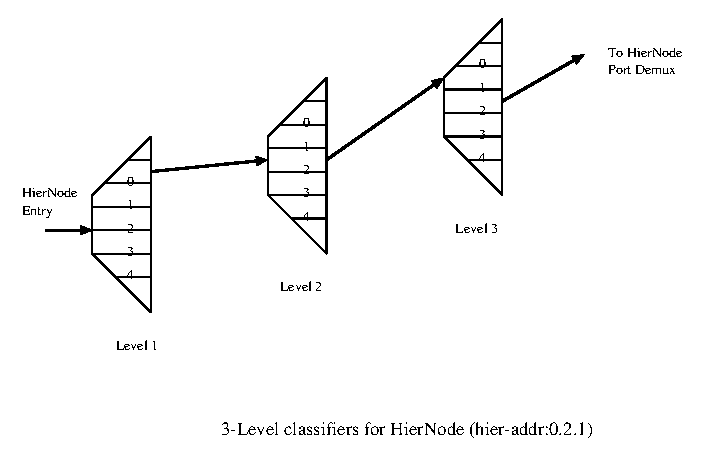
\includegraphics{hier-classifier}}
\caption{Hierarchical classifiers}
\label{fig:hier-classifier}
\end{figure}

Thus the size of the routing tables are considerably reduced from 
$n^{2}$ as seen for flat routing where each node had to store the
  next\_hop info of all other nodes in the topology. Instead, for
  hierarchical routing, a given node needs to know about its neighbours
  in its own cluster, about the all clusters in its domain and about all
  the domains. This saves on memory consumption as well as run-time for
  the simulations using several thousands of nodes in their topology.


\section{Creating large Hierarchical topologies}
\label{large-hier-topo}
The previous section describes methods to create hierarchical topologies
by hand. However, there is a script available in ns that converts
Georgia-tech's SGB-graphs into ns compatible hierarchical topologies.
Please refer to {\em http://www-mash.CS.Berkeley.EDU/ns/ns-topogen.html}
for downloading as well as instructions on using the hierarchical
converter package. 

See hier-rtg-10.tcl and hier-rtg-100.tcl in \nsf{tcl/ex} for example
scripts of hier routing on small and large topologies
respectively. 


\section{Hierarchical Routing with SessionSim}
\label{sec:hier-rtg-with-sessionsim}

Hierarchical routing may be used in conjunction with Session simulations
(see Chapter ~\ref{chap:session}). Session-level simulations which are used
for running multicast simulations over very large topologies, gains
additionally in terms of memory savings if used with hierarchical
routing. See simulation script \nsf{tcl/ex/newmcast/session-hier.tcl}
for an example of sessionsim over hier rtg.


\section{Commands at a glance}

Following is a list of hierarchical routing/addressing related commands
used in simulation scripts:
\begin{flushleft}
\code{$ns_ set-address-format hierarchical}\\
This command was used to setup hierarchical addressing in \ns. However with
the recent changes in node APIs, this command has been replaced by\\
\code{ns_ node-config -addressType hierarchical}\\
This creates a default topology of 3 levels of hierarchy, assigning 8 bits
to each level.


\code{$ns_ set-address-format hierarchical <nlevels> <#bits in level1>....<#bits in level n>}\\
This command creates a hierarchy of <nlevels> and assigns the bits in each level
as specified in the arguments.


\begin{program}
AddrParams set domain_num_ <n_domains>
AddrParams set cluster_num_ <n_clusters>
AddrParams set nodes_num_ <n_nodes>
\end{program}
The above APIs are used to specify the hierarchical topology, i.e the number of
domains, clusters and nodes present in the topology. Default values used by
AddrParams (i.e if nothing is specified) provide a topology with a single
domain with 4 clusters, with each cluster consisting of 5 nodes.


Internal procedures:\\

\code{$Hiernode_ add-hroute <dst> <target>}\\
This procedure is used to add next-hop entries of a destination <dst> for a
given <target>. Since hier-nodes have multiple classifiers, one for each level
of hierarchy, add-hroute populates hier-classifiers correctly and should be
used in place of add-route used for flat-routing.


\code{$hiernode_ split-addrstr <str>}\\
This splits up a hierarchical adrress string  (say a.b.c) into a list of
the addresses at each level (i.e, a,b and c).

\end{flushleft}

\endinput


\part{Transport}
\chapter{UDP Agents}
\label{sec:udpAgents}

\section{UDP Agents}
UDP agents are implemented in \code{udp.\{cc, h\}}.  A UDP agent accepts
data in variable size chunks from an application, and segments the data 
if needed.  UDP packets also contain a monotonically increasing sequence
number.  Although real UDP packets do not contain sequence numbers, this
sequence number does not incur any simulated overhead, and may be useful
for tracefile analysis.

The default maximum segment size (MSS) for UDP agents is 1000 byte:
\begin{program}
Agent/UDP set packetSize_   1000              \; max segment size;
\end{program}
This OTcl instvar is bound to the C++ agent variable \code{size_}.  

Applications can access UDP agents via the \fcn[]{sendmsg} function in C++,
or via the \code{send} or \code{sendmsg} methods in OTcl, as described in
section \ref{sec:systemcalls}.  

The following is a simple example of how a UDP agent may be used in a program.  
In the example, the CBR traffic generator is started at time 1.0, at which time
the generator begins to periodically call the UDP agent \fcn[]{sendmsg}
function.
\begin{program}
        set ns [new Simulator]
        set n0 [$ns node]
        set n1 [$ns node]
        $ns duplex-link $n0 $n1 5Mb 2ms DropTail

        set udp0 [new Agent/UDP]
        $ns attach-agent $n0 $udp0
        set cbr0 [new Application/Traffic/CBR]
        $cbr0 attach-agent $udp0
        $udp0 set packetSize_ 536	\; set MSS to 536 bytes;

        set null0 [new Agent/Null]
        $ns attach-agent $n1 $null0
        $ns connect $udp0 $null0
        $ns at 1.0 "$cbr0 start"
\end{program}
\endinput

\chapter{TCP Agents}
\label{sec:tcpAgents}

This section describes the operation of the TCP agents in \ns.
There are two major types of TCP agents: one-way agents
and a two-way agent.
One-way agents are further subdivided into a set of TCP senders
(which obey different congestion and error control techniques)
and receivers (``sinks'').
The two-way agent is symmetric in the sense that it represents
both a sender and receiver.
It is still under development.

The files described in this section are too numerous to enumerate here.
Basically it covers most files matching the regular expression
\nsf{tcp*.\{cc, h\}}.

The one-way TCP sending agents currently supported are:
\begin{itemize}\itemsep0pt
        \item Agent/TCP - a ``tahoe'' TCP sender
        \item Agent/TCP/Reno - a ``Reno'' TCP sender
        \item Agent/TCP/NewReno - Reno with a modification
        \item Agent/TCP/Sack1 - TCP with selective repeat (follows RFC2018)
        \item Agent/TCP/Vegas - TCP Vegas
        \item Agent/TCP/Fack - Reno TCP with ``forward acknowledgment''
\end{itemize}
The one-way TCP receiving agents currently supported are:
\begin{itemize}\itemsep0pt
        \item Agent/TCPSink - TCP sink with one ACK per packet
        \item Agent/TCPSink/DelAck - TCP sink with configurable delay per ACK
        \item Agent/TCPSink/Sack1 - selective ACK sink (follows RFC2018)
        \item Agent/TCPSink/Sack1/DelAck - Sack1 with DelAck
\end{itemize}
The two-way experimental sender currently supports only a Reno form of TCP:
\begin{itemize}
        \item Agent/TCP/FullTcp
\end{itemize}

The section comprises three parts:
the first part is a simple overview and example of configuring
the base TCP send/sink agents (the sink requires no configuration).
The second part describes the internals of the base send agent,
and last part is a description of the extensions
for the other types of agents that have been included in the
simulator.

\section{One-Way TCP Senders}
\label{sec:oneWayTcp}

The simulator supports several versions of an abstracted TCP sender.
These objects attempt to capture the essence of the TCP congestion
and error control behaviors, but are not intended to be faithful
replicas of real-world TCP implementations.
They do not contain a dynamic window advertisement, they do segment
number and ACK number computations entirely in packet units,
there is no SYN/FIN connection establishment/teardown, and no
data is ever transferred (e.g. no checksums or urgent data).

\subsection{The Base TCP Sender (Tahoe TCP)}
\label{sec:tahoetcp}

The ``Tahoe'' TCP agent \code{Agent/TCP} performs congestion
control and round-trip-time estimation
in a way similar to the version of TCP released with the
4.3BSD ``Tahoe'' UN'X system release from UC Berkeley.
The congestion window is increased by one packet per new ACK received
during slow-start (when $cwnd\_ < ssthresh\_$) and is increased
by $\frac{1}{cwnd\_}$ for each new ACK received during congestion avoidance
(when $cwnd\_ \geq ssthresh\_$).

\paragraph{Responses to Congestion}
Tahoe TCP assumes a packet has been lost (due to congestion)
when it observes {\tt NUMDUPACKS} (defined in \code{tcp.h}, currently 3)
duplicate ACKs, or when a retransmission timer expires.
In either case, Tahoe TCP reacts by setting {\tt ssthresh\_} to half
of the current window size (the minimum of {\tt cwnd\_} and {\tt window\_})
or 2, whichever is larger.
It then initializes {\tt cwnd\_} back to the value of
{\tt windowInit\_}.  This will typically cause the TCP to
enter slow-start.

\paragraph{Round-Trip Time Estimation and RTO Timeout Selection}
Four variables are used to estimate the round-trip time and
set the retransmission timer: {\tt rtt\_, srtt\_, rttvar\_, tcpTick\_,
and backoff\_}.
TCP initializes rttvar to $3/tcpTick\_$ and backoff to 1.
When any future retransmission timer is set, it's timeout
is set to the current time plus $\max(bt(a+4v+1), 64)$ seconds,
where $b$ is the current backoff value, $t$ is the value of tcpTick,
$a$ is the value of srtt, and $v$ is the value of rttvar.

Round-trip time samples arrive with new ACKs.
The RTT sample is computed as the difference between the current
time and a ``time echo'' field in the ACK packet.
When the first sample is taken, its value is used as the initial
value for {\tt srtt\_}.  Half the first sample is used as the initial
value for {\tt rttvar\_}.
For subsequent samples, the values are updated as follows:

\[ srtt = \frac{7}{8} \times srtt + \frac{1}{8} \times sample \]
\[ rttvar = \frac{3}{4} \times rttvar + \frac{1}{4} \times |sample-srtt| \]

\subsection{Configuration}
\label{sec:tcp-config}

Running an TCP simulation requires
creating and configuring the agent,
attaching an application-level data source (a traffic generator), and
starting the agent and the traffic generator.

\subsection{Simple Configuration}

\paragraph{Creating the Agent}
\begin{program}
set ns [new Simulator]                  \; preamble initialization;
set node1 [$ns node]                     \; agent to reside on this node;
set node2 [$ns node]                     \; agent to reside on this node;

{\bfseries{}set tcp1 [$ns create-connection TCP $node1 TCPSink $node2 42]}
$tcp  set window_ 50                   \; configure the TCP agent;

{\bfseries{}set ftp1 [new Application/FTP]}
{\bfseries{}$ftp1 attach-agent $tcp1}

$ns at 0.0 "$ftp start"
\end{program}
This example illustrates the use of the simulator built-in
function {\tt create-connection}.
The arguments to this function are: the source agent to create,
the source node, the target agent to create, the target node, and
the flow ID to be used on the connection.
The function operates by creating the two agents, setting the
flow ID fields in the agents, attaching the source and target agents
to their respective nodes, and finally connecting the agents
(i.e. setting appropriate source and destination addresses and ports).
The return value of the function is the name of the source agent created.

\paragraph{TCP Data Source}
The TCP agent does not generate any application data on its own;
instead, the simulation user can connect any traffic generation
module to the TCP agent to generate data.
Two applications are commonly used for TCP: FTP and Telnet.
FTP represents a bulk data transfer of large size, and telnet chooses
its transfer sizes randomly from tcplib (see the file
\code{tcplib-telnet.cc}.
Details on configuring these application source objects are in
Section~\ref{sec:simapps}.

\subsection{Other Configuration Parameters}

In addition to the \code{window_} parameter listed above,
the TCP agent supports additional configuration variables.
Each of the variables described in this subsection is
both a class variable and an instance variable.
Changing the class variable changes the default value
for all agents that are created subsequently.
Changing the instance variable of a particular agent
only affects the values used by that agent.
For example,
\begin{program}
  Agent/TCP set window_ 100     \; Changes the class variable;
  $tcp set window_ 2.0          \; Changes window_ for the $tcp object only;
\end{program}

The default parameters for each TCP agent are:
\begin{program}
Agent/TCP set window_   20              \; max bound on window size;
Agent/TCP set windowInit_ 1             \; initial/reset value of cwnd;
Agent/TCP set windowOption_ 1           \; cong avoid algorithm (1: standard);
Agent/TCP set windowConstant_ 4         \; used only when windowOption != 1;
Agent/TCP set windowThresh_ 0.002       \; used in computing averaged window;
Agent/TCP set overhead_ 0               \; !=0 adds random time between sends;
Agent/TCP set ecn_ 0                    \; TCP should react to ecn bit ;
Agent/TCP set packetSize_ 1000          \; packet size used by sender (bytes);
Agent/TCP set bugFix_ true              \; see explanation;
Agent/TCP set slow_start_restart_ true  \; see explanation;
Agent/TCP set tcpTick_ 0.1              \; timer granulatiry in sec (.1 is NONSTANDARD);
Agent/TCP set maxrto_ 64                \; bound on RTO (seconds);
Agent/TCP set dupacks_ 0                \; duplicate ACK counter;
Agent/TCP set ack_ 0                    \; highest ACK received;
Agent/TCP set cwnd_ 0                   \; congestion window (packets);
Agent/TCP set awnd_ 0                   \; averaged cwnd (experimental);
Agent/TCP set ssthresh_ 0               \; slow-stat threshold (packets);
Agent/TCP set rtt_ 0                    \; rtt sample;
Agent/TCP set srtt_ 0                   \; smoothed (averaged) rtt;
Agent/TCP set rttvar_ 0                 \; mean deviation of rtt samples;
Agent/TCP set backoff_ 0                \; current RTO backoff factor;
Agent/TCP set maxseq_ 0                 \; max (packet) seq number sent;
\end{program}

For many simulations, few of the configuration parameters are likely
to require modification.
The more commonly modified parameters include: {\tt window\_} and
{\tt packetSize\_}.
The first of these bounds the window TCP uses, and is considered
to play the role of the receiver's advertised window in real-world
TCP (although it remains constant).
The packet size essentially functions like the MSS size in real-world
TCP.
Changes to these parameters can have a profound effect on the behavior
of TCP.
Generally, those TCPs with larger packet sizes, bigger windows, and
smaller round trip times (a result of the topology and congestion) are
more agressive in acquiring network bandwidth.

\subsection{Other One-Way TCP Senders}

\paragraph{Reno TCP}
The Reno TCP agent is very similar to the Tahoe TCP agent,
except it also includes {\em fast recovery}, where the current
congestion window is ``inflated'' by the number of duplicate ACKs
the TCP sender has received before receiving a new ACK.
A ``new ACK'' refers to any ACK with a value higher than the higest
seen so far.
In addition, the Reno TCP agent does not return to slow-start during
a fast retransmit.
Rather, it reduces sets the congestion window to half the current
window and resets {\tt ssthresh\_} to match this value.

\paragraph{NewReno TCP}
This agent is based on the Reno TCP agent, but which modifies the
action taken when receiving new ACKS.
In order to exit fast recovery, the sender must receive an ACK for the
highest sequence number sent.
Thus, new ``partial ACKs'' (those which represent new ACKs but do not
represent an ACK for all outstanding data) do not deflate the window
(and possibly lead to a stall, characteristic of Reno).

\paragraph{Vegas TCP}
This agent implements ``Vegas'' TCP (\cite{Brak94:TCP,Brak94a:TCP}).
It was contributed by Ted Kuo.

\paragraph{Sack TCP}
This agent implements selective repeat, based on selective ACKs provided
by the receiver.
It follows the ACK scheme described in \cite{rfc2018}, and was developed
with Matt Mathis and Jamshid Mahdavi.

\paragraph{Fack TCP}
This agent implements ``forward ACK'' TCP, a modification of Sack
TCP described in \cite{Math96:Forward}.

\section{TCP Receivers (sinks)}

The TCP senders described above represent one-way data senders.
They must peer with a ``TCP sink'' object.

\subsection{The Base TCP Sink}

The base TCP sink object ({\tt Agent/TCPSink})
is responsible for returning ACKs to
a peer TCP source object.
It generates one ACK per packet received.
The size of the ACKs may be configured.
The creation and configuration of the TCP sink object
is generally performed automatically by a library
call (see {\tt create-connection} above).

\paragraph{configuration parameters}
\begin{program}
        Agent/TCPSink set packetSize_ 40
\end{program}

\subsection{Delayed-ACK TCP Sink}

A delayed-ACK sink object ({\tt Agent/Agent/TCPSink/DelAck}) is available
for simulating a TCP receiver that ACKs less than once per packet received.
This object contains a bound variable {\tt interval\_} which gives the
number of seconds to wait between ACKs.
The delayed ACK sink implements an agressive ACK policy whereby
only ACKs for in-order packets are delayed.
Out-of-order packets cause immediate ACK generation.

\paragraph{configuration parameters}
\begin{program}
        Agent/TCPSink/DelAck set interval_ 100ms
\end{program}

\subsection{Sack TCP Sink}

The selective-acknowledgment TCP sink ({\tt Agent/TCPSink/Sack1}) implements
SACK generation modeled after the description of SACK in RFC 2018.
This object includes a bound variable {\tt maxSackBlocks\_} which gives
the maximum number of blocks of information in an ACK available for
holding SACK information.
The default value for this variable is 3, in accordance with the expected
use of SACK with RTTM (see RFC 2018, section 3).
Delayed and selective ACKs together are implemented by
an object of type {\tt Agent/TCPSink/Sack1/DelAck}.

\paragraph{configuration parameters}
\begin{program}
        Agent/TCPSink set maxSackBlocks_ 3
\end{program}

\section{Two-Way TCP Agents (FullTcp)}
\label{sec:fulltcp}

The {\tt Agent/TCP/FullTcp} object is a new addition to the suite of
TCP agents supported in the simulator and is still under development.
It is different from (and incompatible with) the other agents, but
does use some of the same architecture.
It differs from these agents in the following ways:
following ways:
\begin{itemize}\itemsep0pt
\item connections may be establised and town down
(SYN/FIN packets are exchanged)
\item bidirectional data transfer is supported
\item sequence numbers are in bytes rather than packets
\end{itemize}

The generation of SYN packets (and their ACKs) can be
of critical importance in trying to model real-world behavior
when using many very short data transfers.
This version of TCP currently defaults to sending
data on the 3rd segment of an initial 3-way handshake, a behavior
somewhat different than common real-world TCP implementations.
A ``typical'' TCP connection proceeds with an active opener
sending a SYN, the passive opener responding with a SYN+ACK,
the active opener responding with an ACK, and then some time later
sending the first segment with data (corresponding to the first
application write).
Thus, this version of TCP sends data at a time somewhat earlier
than typical implementations.
This TCP can also be configured to send data on the initial SYN
segment.
Future changes to FullTCP may include a modification to send the
first data segment later, and possibly to implement T/TCP functionality.

Currently FullTCP is only implemented with Reno congestion control,
but ultimately it should be available with the full range of
congestion control algorithms (e.g., Tahoe, SACK, Vegas, etc.).


\subsection{Simple Configuration}
Running an Full TCP simulation requires
creating and configuring the agent,
attaching an application-level data source (a traffic generator), and
starting the agent and the traffic generator.

\paragraph{Creating the Agent}
\begin{program}
# {\cf set up connection (do not use "create-connection" method because }
# {\cf we need a handle on the sink object)}
set src [new Agent/TCP/FullTcp] \; create agent;
set sink [new Agent/TCP/FullTcp] \; create agent;
$ns_ attach-agent $node_(s1) $src \; bind src to node;
$ns_ attach-agent $node_(k1) $sink \; bind sink to node;
$src set fid_ 0   \; set flow ID field;
$sink set fid_ 0  \; set flow ID field;
$ns_ connect $src $sink \; active connection src to sink;

# {\cf set up TCP-level connections}
$sink listen \; will figure out who its peer is;
$src set window_ 100;
\end{program}

The creation of the FullTcp agent is similar to the other agents,
but the sink is placed in a listening state by the {\tt listen} method.
Because a handle to the receiving side is required in order to make
this call, the {\tt create-connection} call used above cannot be used.

\paragraph{Configuration Parameters}
The following configuration parameters are available through Tcl
for the FullTcp agent:
\begin{program}
Agent/TCP/FullTcp set segsperack_ 1 \; segs received before generating ACK;
Agent/TCP/FullTcp set segsize_ 536  \; segment size (MSS size for bulk xfers);
Agent/TCP/FullTcp set tcprexmtthresh_ 3 \; dupACKs thresh to trigger fast rexmt;
Agent/TCP/FullTcp set iss_ 0 \; initial send sequence number;
Agent/TCP/FullTcp set nodelay_ false \; disable sender-side Nagle algorithm;
Agent/TCP/FullTcp set data_on_syn_ false \; send data on initial SYN?;
Agent/TCP/FullTcp set dupseg_fix_ true \; avoid fast rxt due to dup segs+acks;
Agent/TCP/FullTcp set dupack_reset_ false \; reset dupACK ctr on !0 len data segs containing dup ACKs;
Agent/TCP/FullTcp set interval_ 0.1 \; as in TCP above, (100ms is non-std);
\end{program}

\section{Architecture and Internals}
\label{sec:tcparchitecture}

The base TCP agent (class {\tt Agent/TCP}) is constructed
as a collection of routines for sending packets, processing ACKs,
managing the send window, and handling timeouts.
Generally, each of these routines may be over-ridden by a
function with the same name in a derived class (this is how
many of the TCP sender variants are implemented).

\paragraph{The TCP header}
The TCP header is defined by the {\tt hdr\_tcp} structure
in the file \nsf{tcp.h}.
The base agent only makes use of the following subset of the fields:
\begin{program}
ts_     \* current time packet was sent from source */
ts_echo_ \* for ACKs: timestamp field from packet associated with this ACK */
seqno_ \* sequence number for this data segment or ACK (Note: overloading!) */
reason_ \* set by sender when (re)transmitting to trace reason for send */
\end{program}

\paragraph{Functions for Sending Data}
Note that generally the sending TCP never actually sends
data (it only sets the packet size).

{\bf send\_much(force, reason, maxburst)} - this function
attempts to send as many packets as the current sent window allows.
It also keeps track of how many packets it has sent, and limits to the
total to {\em maxburst}. \\
The function {\tt output(seqno, reason)} sends one packet
with the given sequence number and updates the maximum sent sequence
number variable ({\tt maxseq\_}) to hold the given sequence number if
it is the greatest sent so far.
This function also assigns the various fields in the TCP
header (sequence number, timestamp, reason for transmission).
This function also sets a retransmission timer if one is not already
pending.

\paragraph{Functions for Window Management}

The usable send window at any time is given by the function {\bf window()}.
It returns the minimum of the congestion window and the variable {\tt wnd\_},
which represents the receiver's advertised window.

{\bf opencwnd()} - this function opens the congestion window.  It is invoked
when a new ACK arrives.
When in slow-start, the function merely increments {\tt cwnd\_} by each
ACK received.
When in congestion avoidance, the standard configuration increments {\tt cwnd\_}
by its reciprocal.
Other window growth options are supported during congestion avoidance,
but they are experimental (and not documented; contact Sally Floyd for
details).

{\bf closecwnd(int how)} - this function reduces the congestion window. It
may be invoked in several ways: when entering fast retransmit, due to
a timer expiration, or due to a congestion notification (ECN bit set).
Its argument {\tt how} indicates how the congestion window should
be reduced.  The value {\bf 0} is used for retransmission timeouts and
fast retransmit in Tahoe TCP.  It typically causes the TCP to enter
slow-start and reduce {\tt ssthresh\_} to half the current window.
The value {\bf 1} is used by Reno TCP for implementing fast recovery
(which avoids returning to slow-start).
The value {\bf 2} is used for reducing the window due to an ECN indication.
It resets the congestion window to its initial value (usually causing
slow-start), but does not alter {\tt ssthresh\_}.

\paragraph{Functions for Processing ACKs}

{\bf recv()} - this function is the main reception path for ACKs.
Note that because only one direction of data flow is in use, this function
should only ever be invoked with a pure ACK packet (i.e. no data).
The function stores the timestamp from the ACK in {\tt ts\_peer\_}, and
checks for the presence of the ECN bit (reducing the send window if
appropriate).
If the ACK is a new ACK, it calls {\bf newack()}, and otherwise
checks to see if it is a duplicate of the last ACK seen.
If so, it enters fast retransmit by closing the window, resetting the
retransmission timer, and sending a packet by calling {\tt send\_much}.

{\bf newack()} - this function processes a ``new'' ACK (one that contains
an ACK number higher than any seen so far).
The function sets a new retransmission timer by calling {\bf newtimer()},
updates the RTT estimation by calling {\bf rtt\_update}, and updates
the highest and last ACK variables.

\paragraph{Functions for Managing the Retransmission Timer}

These functions serve two purposes: estimating the round-trip time
and setting the actual retransmission timer.
{\bf rtt\_init} - this function initializes {\tt srtt\_} and {\tt rtt\_}
to zero, sets {\tt rttvar\_} to $3/tcp\_tick\_$, and sets the backoff
multiplier to one.

{\bf rtt\_timeout} - this function gives the timeout value in seconds that
should be used to schedule the next retransmission timer.
It computes this based on the current estimates of the mean and deviation
of the round-trip time.  In addition, it implements Karn's
exponential timer backoff for multiple consecutive retransmission timeouts.

{\bf rtt\_update} - this function takes as argument the measured RTT
and averages it in to the running mean and deviation estimators
according to the description above.
Note that {\tt t\_srtt\_} and {\tt t\_rttvar} are both
stored in fixed-point (integers).
They have 3 and 2 bits, respectively, to the right of the binary
point.

{\bf reset\_rtx\_timer} -  This function is invoked during fast retransmit
or during a timeout.
It sets a retransmission timer
by calling {\tt set\_rtx\_timer} and if invoked by a timeout also calls
{\tt rtt\_backoff}.

{\bf rtt\_backoff} - this function backs off the retransmission timer
(by doubling it).

{\bf newtimer} - this function called only when a new ACK arrives.
If the sender's left window edge is beyond the ACK, then
{\tt set\_rtx\_timer} is called, otherwise if a retransmission timer
is pending it is cancelled.

\section{Tracing TCP Dynamics}
\label{sec:traceTcpdyn}

The behavior of TCP is often observed by constructing a
sequence number-vs-time plot.
Typically, a trace is performed by enabling tracing on a link
over which the TCP packets will pass.
Two trace methods are supported: the default one (used for tracing
TCP agents), and an extension used only for FullTcP.

\section{One-Way Trace TCP Trace Dynamics}
\label{sec:trace1WayTcpdyn}

TCP packets generated by one of the one-way TCP agents and destined for
a TCP sink agent
passing over a traced link (see section~\ref{chap:trace})
will generate a trace file lines of the form:
\begin{verbatim}
+ 0.94176 2 3 tcp 1000 ------ 0 0.0 3.0 25 40
+ 0.94276 2 3 tcp 1000 ------ 0 0.0 3.0 26 41
d 0.94276 2 3 tcp 1000 ------ 0 0.0 3.0 26 41
+ 0.95072 2 0 ack 40 ------ 0 3.0 0.0 14 29
- 0.95072 2 0 ack 40 ------ 0 3.0 0.0 14 29
- 0.95176 2 3 tcp 1000 ------ 0 0.0 3.0 21 36
+ 0.95176 2 3 tcp 1000 ------ 0 0.0 3.0 27 42
\end{verbatim}
The exact format of this trace file is given in section~\ref{sec:traceformat}.
When tracing TCP, packets of type {\sf tcp} or {\sf ack} are relevant.
Their type, size, sequence number (ack number for ack packets),
and arrival/depart/drop time are given by field positions
5, 6, 11, and 2, respectively.
The {\sf +} indicates a packet arrival, {\sf d} a drop, and {\sf -} a
departure.
A number of scripts process this file to produce graphical output or
statistical summaries (see,  for example, \nsf{test-suite.tcl}, the
{\tt finish} procedure.

\section{One-Way Trace TCP Trace Dynamics}
\label{sec:tcpdyn}

TCP packets generated by FullTcp and
passing over a traced link contain additional information not displayed
by default using the regular trace object.
By enabling the flag {\tt show\_tcphdr\_} on the trace object
(see section~ref{sec:traceformat}), 3 additional header fields are
written to the trace file: ack number, tcp-specific flags, and header length.

\endinput

\documentclass{article}

\usepackage{times}
\usepackage[T1]{fontenc}

\PassOptionsToPackage{draft}{nsDoc}
\usepackage{nsDoc}

\begin{document}

\title{\nsTcl\ internals documentation}
\author{%
  Various members of the VINT project \tup{vint@catarina.usc.edu}\\
  Kevin Fall \tup{kfall@ee.lbl.gov}, Editor,\\
  Kannan Varadhan \tup{kannan@catarina.usc.edu}, Editor.}
\date{\today}

\def\c#1{\ensuremath{C_{#1}}}
\def\d#1{\ensuremath{D_{#1}}}

% \maketitle

\section{Agent/SRM}
\label{sec:agent/srm}

This section describes the internals of the SRM implementation in \ns.
The section is in three parts:
the first part is an overview of a minimal SRM configuration,
and a ``complete'' description of the configuration parameters 
of the base SRM agent.
The second part describes the architecture, internals, and the code path
of the base SRM agent.
The last part of the section is a description of the extensions
for other types of SRM agents that have been attempted to date.

\subsection{Configuration}
\label{sec:srm-config}

Running an SRM simulation requires
creating and configuring the agent,
attaching an application-level data source (a traffic generator), and
starting the agent and the traffic generator.

\subsubsection{Trivial Configuration}

\paragraph{Creating the Agent}
\begin{program}
        set ns [new Simulator]          \; preamble initialization;
        $ns enableMcast
        set node [$ns node]                \; agent to reside on this node;
        set group [$ns allocaddr]           \; multicast group for this agent;

        {\bfseries{}set srm [new Agent/SRM]}
        $srm  set dst_ $group            \; configure the SRM agent;
        {\bfseries{}$ns attach-agent $node $srm}

        $srm set fid_ 1                \; optional configuration;
        $srm log [open srmStats.tr w]   \; log statistics in this file;
        $srm trace [open srmEvents.tr w]  \; trace events for this agent;
\end{program}
The key steps in configuring a virgin SRM agent are to assign
its multicast group, and attach it to a node.

Other useful configuration parameters are
to assign a separate flow id to traffic originating from this agent,
to open a log file for statistics, and
a trace file for trace data%
\footnote{%
Note that the trace data can also be used
to gather certain kinds of trace data.
We will illustrate this later.}.

The file
\fcnref{\|tcl/mcast/srm-nam.tcl|}{../ns-2/srm-nam.tcl}{Agent/SRM::send}
contains definitions that overload the agent's \|send| methods;
this separates control traffic originating from the agent by type.
Each type is allocated a separate flowID.
The traffic is separated into session messages (flowid = 40),
requests (flowid = 41), and repair messages (flowid = 42).
The base flowid can be changed by setting global variable \|ctrlFid|
to one less than the desired flowid before sourcing \|srm-nam.tcl|.
To do this, the simulation script must source \|srm-nam.tcl|
before creating any SRM agents.
This is useful for analysis of traffic traces, or
for visualization in nam.

\paragraph{Application Data Handling}
The agent does not generate any application data on its own;
instead, the simulation user can connect any traffic generation
module to any SRM agent to generate data.
The following code demonstrates
how a traffic generation agent can be attached to an SRM agent:
\begin{program}
        set packetSize 210
        set exp0 [new Traffic/Expoo]    \; configure traffic generator;
        $exp0 set packet-size $packetSize
        $exp0 set burst-time 500ms 
        $exp0 set idle-time 500ms
        $exp0 set rate 100k 

        set s0 [new Agent/CBR/UDP]   \; attach traffic generator to application;
        $s0 set fid_ 0
        $s0 attach-traffic $exp0

        {\bfseries{}$srm(0) traffic-source $s0} \; attach application to SRM agent;
        {\bfseries{}$srm(0) set packetSize_ $packetSize} \; to generate repair packets of appropriate size;
\end{program}
The instproc \texttt{\textbf{traffic-source}} specifies the application agent
that will produce data for the SRM agent.
The user can attach any agent;
the only distinguishing criteria is that the destination address must be zero.
The SRM agent will add the SRM headers, 
set the destination address to the multicast group, and
deliver the packet to its target.
The SRM header contains the type of the message,
the identity of the sender,
the sequence number of the message,
and (for control messages), the round for which this message is being sent.
Each data unit in SRM is identified as
\tup{sender's id, message sequence number}.

The SRM agent does not generate its own data;
it does not also keep track of the data sent,
except to record the sequence numbers of messages received
in the event that it has to do error recovery.
Since the agent has no actual record of past data,
it needs to know what packet size to use for each repair message.
Hence, the instance variable \|packetSize_| specifies the size
of repair messages generated by the agent.

\paragraph{Starting the Agent and Traffic Generator}
The agent and the traffic generator must be started separately.
\begin{program}
        {\bfseries{}\fcnref{$srm start}{../ns-2/srm.tcl}{Agent/SRM::start}}
        {\bfseries{}\fcnref{$srm start-source}{../ns-2/srm.tcl}{Agent/SRM::start-source}}
\end{program}
At \|start|, the agent joins the multicast group, and 
starts generating session messages.
The \|start-source| triggers the traffic generator to start sending
data.

\subsubsection{Other Configuration Parameters}
\label{sec:config-param}

In addition to the above parameters,
the SRM agent supports additional configuration variables.
Each of the variables described in this subsection is
both an OTcl class variable and an OTcl object's instance variable.
Changing the class variable changes the default value
for all agents that are created subsequently.
Changing the instance variable of a particular agent
only affects the values used by that agent.
For example,
\begin{program}
                Agent/SRM set D1_ 2.0 \; Changes the class variable;
                $srm set D1_ 2.0        \; Changes D1_ for the particular $srm object only;
\end{program}

The default request and repair timer parameters \cite{Floy95:Reliable}
for each SRM agent are:
\begin{program}
        Agent/SRM set C1_       2.0 \; request parameters;
        Agent/SRM set C2_       2.0
        Agent/SRM set D1_       1.0 \; repair parameters;
        Agent/SRM set D2_       1.0
\end{program}
It is thus possible to trivially obtain two flavours of SRM agents
based on whether the agents use probabilistic or deterministic
suppression by using the following definitions:
\begin{program}
        Class Agent/SRM/Deterministic -superclass Agent/SRM
        Agent/SRM/Deterministic set C2_ 0.0
        Agent/SRM/Deterministic set D2_ 0.0

        Class Agent/SRM/Probabilistic -superclass Agent/SRM
        Agent/SRM/Probabilistic set C1_ 0.0
        Agent/SRM/Probabilistic set D1_ 0.0
\end{program}
In \href{a later section}{Section}{sec:extensions},
we will discuss other ways of extending the SRM agent.

Timer related functions are handled by separate objects
belonging to the class  SRM.
Timers are required for loss recovery and sending periodic session messages.
There are loss recovery objects to send request and repair messages.
The agent creates a separate request or repair object to handle each loss.
In contrast, the agent only creates one session object to send
periodic session messages.
The default classes the express each of these functions are:
\begin{program}
        Agent/SRM set requestFunction_  "SRM/request"
        Agent/SRM set repairFunction_   "SRM/repair"
        Agent/SRM set sessionFunction_  "SRM/session"

        Agent/SRM set requestBackoffLimit_      5       \; parameter to requestFunction_;
        Agent/SRM set sessionDelay_             1.0     \; parameter to sessionFunction_;
\end{program}
The instance procedures
\fcnref{\proc[]{requestFunction}}{../ns-/srm.tcl}{Agent/SRM::requestFunction},
\fcnref{\proc[]{repairFunction}}{../ns-/srm.tcl}{Agent/SRM::repairFunction},
and
\fcnref{\proc[]{sessionFunction}}{../ns-/srm.tcl}{Agent/SRM::sessionFunction}
can be used to change the default function for individual agents.
The last two lines are specific parameters used by the request 
and session objects.
The \href{following section}{Section}{sec:architecture}
describes the implementation of theses objects in greater detail.

\subsubsection{Statistics}
Each agent tracks two sets of statistics:
statistics to measure the response to data loss,
and overall statistics for each request/repair.
In addition, there are methods to access other
information from the agent.

\paragraph{Data Loss}
The statistics to measure the response to data losses
tracks the duplicate requests (and repairs),
and the average request (and repair) delay.
The algorithm used is documented in Floyd \etal \cite{Floy95:Reliable}.
In this algorithm,
each new request (or repair) starts a new request (or repair) period.
During the request (or repair) period, the agent measures
the number of first round duplicate requests (or repairs)
until the round terminates either due to receiving a request (or
repair), or due to the agent sending one.
% These statistics are used by the adaptive timer algorithms;
% we will describe our implementation of these algorithms
% in the following subsections.
The following code illustrates how the user can simple retrieve the
current values in an agent:
\begin{program}
                set statsList [$srm array get statistics_]
                array set statsArray [$srm array get statistics_]
\end{program}
The first form returns a list of key-value pairs.
The second form loads the list into the \|statsArray| for further manipulation.
The keys of the array are
\|dup-req|, \|ave-dup-req|, \|req-delay|, \|ave-req-delay|,
\|dup-rep|, \|ave-dup-rep|, \|rep-delay|, and \|ave-rep-delay|.

\paragraph{Overall Statistics}
In addition, each loss recovery and session object keeps track of
times and statistics.
In particular, each object records its
\|startTime|, \|serviceTime|, \|distance|, as are relevant to that object;
startTime is the time that this object was created,
serviceTime is the time for this object to complete its task, and the
distance is the one-way time to reach the remote peer.

For request objects, startTime is the time a packet loss is detected,
serviceTime is the time to finally receive that packet,
and distance is the distance to the original sender of the packet.
For repair objects, startTime is the time that a request for
retransmission is received, serviceTime is the time send a repair,
and the distance is the distance to the original requester.
For both types of objects, the serviceTime is normalised by the
distance.
For  the session object,
startTime is the time that the agent joins the multicast group.
serviceTime and distance are not relevant.

Each object also maintains statistics particular to that type of object.
Request objects track the number of duplicate requests and repairs received,
the number of requests sent, and the number of times this object
had to backoff before finally receiving the data.
Repair objects track the number of duplicate requests and repairs,
as well as whether or not this object for this agent sent the repair.
Session objects simply record the number of session messages sent.

The values of the timers and the statistics for each object are written
to the log file every time an object completes the error recovery function
it was tasked to do.
The format of this trace file is:
\begin{program}
                \tup{prefix} \tup{id} \tup{times} \tup{stats}
{\itshape{}where}
\tup{prefix} is         \tup{time} n \tup{node id} m \tup{msg id} r \tup{round}
                \tup{msg id} is expressed as \tup{source id:sequence number}
\tup{id} is             type \tup{of object}
\tup{times} is          list of key-value pairs of startTime, serviceTime, distance
\tup{stats} is          list of key-value pairs of per object statistics
                \|dupRQST|, \|dupREPR|, \|#sent|, \|backoff|             {\itshape for request objects}
                \|dupRQST|, \|dupREPR|, \|#sent|                      {\itshape for repair objects}
                \|#sent|                                        {\itshape for session objects}
\end{program}
The following sample output illustrates the output file format (the lines
have been folded to fit on the page):
{\small
\begin{verbatim}
 3.6274 n 0 m <1:1> r 1 type repair serviceTime 0.500222 \
        startTime 3.5853553333333332 distance 0.0105 #sent 1 dupREPR 0 dupRQST 0
 3.6417 n 1 m <1:1> r 2 type request serviceTime 2.66406 \
        startTime 3.5542666666666665 distance 0.0105 backoff 1 #sent 1 dupREPR 0 dupRQST 0
 3.6876 n 2 m <1:1> r 2 type request serviceTime 1.33406 \
        startTime 3.5685333333333333 distance 0.021 backoff 1 #sent 0 dupREPR 0 dupRQST 0
 3.7349 n 3 m <1:1> r 2 type request serviceTime 0.876812 \
        startTime 3.5828000000000002 distance 0.032 backoff 1 #sent 0 dupREPR 0 dupRQST 0
 3.7793 n 5 m <1:1> r 2 type request serviceTime 0.669063 \
        startTime 3.5970666666666671 distance 0.042 backoff 1 #sent 0 dupREPR 0 dupRQST 0
 3.7808 n 4 m <1:1> r 2 type request serviceTime 0.661192 \
        startTime 3.5970666666666671 distance 0.0425 backoff 1 #sent 0 dupREPR 0 dupRQST 0
\end{verbatim}
}

\paragraph{Miscellaneous Information}
Finally, the user can use the following methods to gather
additional information about the agent:
\begin{list}{\textbullet}{}
\item
  \fcnref{\proc[]{groupSize?}}{../ns-2/srm.tcl.html}{Agent/SRM::groupSize?} 
  returns the agent's current estimate of the multicast group size.
\item
  \fcnref{\proc[]{distances?}}{../ns-2/srm.cc.html}{SRMAgent::command}
  returns a list of key-value pairs of distances;
  the key is the address of the agent, 
  the value is the estimate of the distance to that agent.
  The first element is the address of this agent, and the distance of 0.
\item
  \fcnref{\proc[]{distance?}}{../ns-2/srm.cc.html}{SRMAgent::command}
  returns the distance to the particular agent specified as argument.

  The default distance at the start of any simulation is 1.
\end{list}
\begin{program}
        $srm(i) groupSize?    \; returns $srm(i)'s estimate of the group size;
        $srm(i) distances?    \; returns list of \tup{address, distance} tuples;
        $srm(i) distance? 257 \; returns the distance to agent at address 257;
\end{program}

\subsubsection{Tracing}
Each object writes out trace information that can be used to track the
progress of the object in its error recovery.
Each trace entry is of the form:
\begin{program}
\tup{prefix} \tup{tag} \tup{type of entry} \tup{values}
\end{program}
The prefix is as describe in the previous subsection for statistics.
The tag is {\bf Q} for request objects, {\bf P} for repair objects, and
{\bf S} for session objects.
The following types of trace entries and parameters are written by each
object:

\centerline{\small\renewcommand{\arraystretch}{1.3}
\begin{tabular}{rclp{2in}}\hline
      & Type of &              & \\
  Tag & Object  & Other values & Comments\\ \hline
  Q & DETECT & & \\
  Q & INTERVALS & C1 \tup{C1\_} C2 \tup{C2\_} dist \tup{distance} i \tup{backoff\_} & \\
  Q & NTIMER & at \tup{time} & Time the request timer will fire \\
  Q & SENDNACK & & \\
  Q & NACK & IGNORE-BACKOFF \tup{time} & Receive NACK, ignore other NACKs until
  \tup{time} \\
  Q & REPAIR & IGNORES \tup{time} & Receive REPAIR, ignore NACKs until \tup{time}  \\
  Q & DATA & & Agent receives data instead of repair.  Possibly indicates out of order arrival of data. \\ \hline
  P & NACK & from \tup{requester} & Receive NACK, initiate repair \\
  P & INTERVALS & D1 \tup{D1\_} D2 \tup{D2\_} dist \tup{distance} & \\
  P & RTIMER & at \tup{time} & Time the repair timer will fire \\
  P & SENDREP & \\
  P & REPAIR & IGNORES \tup{time} & Receive REPAIR, ignore NACKs until \tup{time} \\
  P & DATA & & Agent receives data instead of repair.  Indicates premature request by an agent. \\ \hline
  S & SESSION & & logs session message sent \\ \hline
\end{tabular}}
The following illustrates a typical trace for a single loss and recovery.
{\small
\begin{verbatim}
 3.5543 n 1 m <1:1> r 0 Q DETECT
 3.5543 n 1 m <1:1> r 1 Q INTERVALS C1 2.0 C2 0.0 d 0.0105 i 1
 3.5543 n 1 m <1:1> r 1 Q NTIMER at 3.57527
 3.5685 n 2 m <1:1> r 0 Q DETECT
 3.5685 n 2 m <1:1> r 1 Q INTERVALS C1 2.0 C2 0.0 d 0.021 i 1
 3.5685 n 2 m <1:1> r 1 Q NTIMER at 3.61053
 3.5753 n 1 m <1:1> r 1 Q SENDNACK
 3.5753 n 1 m <1:1> r 2 Q INTERVALS C1 2.0 C2 0.0 d 0.0105 i 2
 3.5753 n 1 m <1:1> r 2 Q NTIMER at 3.61727
 3.5753 n 1 m <1:1> r 2 Q NACK IGNORE-BACKOFF 3.59627
 3.5828 n 3 m <1:1> r 0 Q DETECT
 3.5828 n 3 m <1:1> r 1 Q INTERVALS C1 2.0 C2 0.0 d 0.032 i 1
 3.5828 n 3 m <1:1> r 1 Q NTIMER at 3.6468
 3.5854 n 0 m <1:1> r 0 P NACK from 257
 3.5854 n 0 m <1:1> r 1 P INTERVALS D1 1.0 D2 0.0 d 0.0105
 3.5854 n 0 m <1:1> r 1 P RTIMER at 3.59586
 3.5886 n 2 m <1:1> r 2 Q INTERVALS C1 2.0 C2 0.0 d 0.021 i 2
 3.5886 n 2 m <1:1> r 2 Q NTIMER at 3.67262
 3.5886 n 2 m <1:1> r 2 Q NACK IGNORE-BACKOFF 3.63062
 3.5959 n 0 m <1:1> r 1 P SENDREP
 3.5959 n 0 m <1:1> r 1 P REPAIR IGNORES 3.62736
 3.5971 n 4 m <1:1> r 0 Q DETECT
 3.5971 n 4 m <1:1> r 1 Q INTERVALS C1 2.0 C2 0.0 d 0.0425 i 1
 3.5971 n 4 m <1:1> r 1 Q NTIMER at 3.68207
 3.5971 n 5 m <1:1> r 0 Q DETECT
 3.5971 n 5 m <1:1> r 1 Q INTERVALS C1 2.0 C2 0.0 d 0.042 i 1
 3.5971 n 5 m <1:1> r 1 Q NTIMER at 3.68107
 3.6029 n 3 m <1:1> r 2 Q INTERVALS C1 2.0 C2 0.0 d 0.032 i 2
 3.6029 n 3 m <1:1> r 2 Q NTIMER at 3.73089
 3.6029 n 3 m <1:1> r 2 Q NACK IGNORE-BACKOFF 3.66689
 3.6102 n 1 m <1:1> r 2 Q REPAIR IGNORES 3.64171
 3.6172 n 4 m <1:1> r 2 Q INTERVALS C1 2.0 C2 0.0 d 0.0425 i 2
 3.6172 n 4 m <1:1> r 2 Q NTIMER at 3.78715
 3.6172 n 4 m <1:1> r 2 Q NACK IGNORE-BACKOFF 3.70215
 3.6172 n 5 m <1:1> r 2 Q INTERVALS C1 2.0 C2 0.0 d 0.042 i 2
 3.6172 n 5 m <1:1> r 2 Q NTIMER at 3.78515
 3.6172 n 5 m <1:1> r 2 Q NACK IGNORE-BACKOFF 3.70115
 3.6246 n 2 m <1:1> r 2 Q REPAIR IGNORES 3.68756
 3.6389 n 3 m <1:1> r 2 Q REPAIR IGNORES 3.73492
 3.6533 n 4 m <1:1> r 2 Q REPAIR IGNORES 3.78077
 3.6533 n 5 m <1:1> r 2 Q REPAIR IGNORES 3.77927
\end{verbatim}
The logging of request and repair traces is done by
\fcnref{\proc[]{SRM::evTrace}}{../ns-2/srm.tcl}{SRM::evTrace}.
However, the routine
\fcnref{\proc[]{SRM/Session::evTrace}}{../ns-2/srm.tcl}{SRM/Session::evTrace},
overrides the base class definition of \proc[]{srm::evTrace},
and writes out nothing.
Individual simulation scripts can override these methods
for greater flexibility in logging options.
One possible reason to override these methods might to
reduce the amount of data generated;
the new procedure could then generate compressed and processed output.

Notice that the trace filoe contains sufficient information and details
to derive most of the statistics written out in the log file, or
is stored in the statistics arrays.

\subsection{Architecture and Internals}
\label{sec:architecture}

The SRM agent implementation splits the protocol functions
into packet handling, loss recovery, and session message activity.
\begin{list}{}{}
\item  Packet handling consists of forwarding application data messages,
  sending and receipt of control messages.
  These activities are executed by C++ methods.
\item  Error detection is done in C++ due to receipt of messages.
  However, the loss recovery is entirely done through 
  instance procedures in OTcl.
\item  The sending and processing of messages is accomplished in C++;
  the policy about when these messages should be sent is decided
  by instance procedures in OTcl.
\end{list}
We first describe the C++
\href{processing due to receipt of messages}{Section}{sec:reciept}.
Loss recovery and the sending of session messages involves
timer based processing.
The agent uses a separate \clsref{SRM}{../ns-2/srm.tcl}
to perform the timer based functions.
For each loss, an agent may do either request or repair processing.
Each agent will instantiate a separate loss recovery object
for every loss, as is appropriate for the processing that it has to do.
In the following section
\href{we describe the basic timer based functions and
the loss recovery mechanisms}{Section}{sec:recovery}.
Finally, each agent uses one timer based function
for \href{sending periodic session messages}{Section}{sec:session}.

\subsection{Packet Handling: Processing received messages}
\label{sec:reciept}

The
\fcnref{\fcn[]{recv}}{../ns-2/srm.cc}{SRMAgent::recv}
method can receive four type of messages:
data, request, repair, and session messages.

\paragraph{Data Packets}
The agent does not generate any data messages.
The user has to specify an external agent to generate traffic.
The \fcn[]{recv} method must distinguish between
locally originated data that must be sent to the multicast group,
and data received from multicast group that must be processed.
Therefore, the application agent must
set the packet's destination address to zero.

For locally originated data, 
the agent adds the appropriate SRM headers,
sets the destination address to the multicast group, 
and forwards the packet to its target.

On receiving a data message from the group,
\fcnref{\fcn[sender, msgid]{recv\_data}}{../ns-2/srm.cc}{SRMAgent::recv\_data}
will update its state marking message \tup{sender, msgid} received,
and possibly trigger requests if it detects losses.
In addition, if the message was an older message received out of order,
then there must be a pending request or repair that must be cleared.
In that case, the compiled object invokes the OTcl instance procedure,
\fcnref{\proc[sender, msgid]{recv-data}}{%
  ../ns-2/srm.tcl}{Agent/SRM::recv-data}%
\footnote{Technically,
  \fcn[]{recv\_data} invokes the instance procedure
  \|recv data \tup{sender} \tup{msgid}|,
  that then invokes \proc[]{recv-data}.
  The indirection allows individual simulation scripts to override the
  \proc[]{recv} as needed.}.

Currently, there is no provision for the receivers
to actually receive any application data.
The agent does not also store any of the user data.
It only generates repair messages of the appropriate size,
defined by the instance variable \|packetSize_|.
However, the agent assumes that any application data
is placed in the data portion of the packet,
pointed to by \|packet->accessdata()|.

\paragraph{Request Packets}
On receiving a request, 
\fcnref{\fcn[sender, msgid]{recv\_rqst}}{../ns-2/srm.cc}{SRMAgent::recv\_rqst}
will check whether it needs to schedule requests for other missing data.
If it has received this request
before it was aware that the source had generated this data message
(\ie, the sequence number of the request is higher than 
the last known sequence number of data from this source),
then the agent can infer that it is missing this, as well as data
from the last known sequence number onwards;
it schedules requests for all of the missing data and returns.
On the other hand, if the sequence number of the request is less
than the last known sequence number from the source,
then the agent can be in one of three states:
(1) it does not have this data, and has a request pending for it,
(2) it has the data, and has seen an earlier request,
    upon which it has a repair pending for it, or
(3) it has the data, and it should instantiate a repair.
All of these error recovery mechanisms are done in OTcl;
\fcn[]{recv\_rqst} invokes the instance procedure
\fcnref{\proc[sender, msgid,
  requester]{recv-rqst}}{../ns-2/srm.tcl}{Agent/SRM::recv-rqst}
for further processing.

\paragraph{Repair Packets}
On receiving a repair, 
\fcnref{\fcn[sender, msgid]{recv\_repr}}{../ns-2/srm.cc}{SRMAgent::recv\_repr}
will check whether it needs to schedule requests for other missing data.
If it has received this repair
before it was aware that the source had generated this data message
(\ie, the sequence number of the repair is higher than 
the last known sequence number of data from this source),
then the agent can infer that it is missing all
data between the last known sequence number and that on the repair;
it schedules requests for all of this data,
 marks this message as received, and returns.
On the other hand, if the sequence number of the request is less
than the last known sequence number from the source,
then the agent can be in one of three states:
(1) it does not have this data, and has a request pending for it,
(2) it has the data, and has seen an earlier request,
    upon which it has a repair pending for it, or
(3) it has the data, and probably scheduled a repair for it at some time;
    after error recovery, its holddown timer (equal to three times its
    distance to some requestor) expired, at which time the pending object
    was cleared.  In this last situation, the agent will simply ignore
    the repair, for lack of being able to do anything meaningful.
All of these error recovery mechanisms are done in OTcl;
\fcn[]{recv\_repr} invokes the instance procedure
\fcnref{\proc[sender, msgid]{recv-repr}}{%
  ../ns-2/srm.tcl}{Agent/SRM::recv-rqst}
to complete the loss recovery phase for the particular message.
  
\paragraph{Session Packets}
On receiving a session message,
the agent updates its sequence numbers for all active sources,
and computes its instantaneous distance to the sending agent if possible.
The agent will ignore earlier session messages from a group member,
if it has received a later one out of order.
  
Session message processing is done in
\fcnref{\fcn[]{recv\_sess}}{../ns-2/srm.cc}{SRMAgent::recv\_sess}.
The format of the session message is:
\tup{count of tuples in this message, list of tuples},
where each tuple indicates the
\tup{sender id, last sequence number from the source, time the last
  session message was received from this sender, time that that message
  was sent}.
The first tuple is the information about the local agent%
\footnote{Note that this implementation of session message handling
  is subtly different from that used in \emph{wb} or described in
  \cite{Floy95:Reliable}.
  In principle, an agent disseminates a list of the data it has
  actually received.
  Our implementation, on the other hand, only disseminates
  a count of the last message sequence number per source that the
  agent knows that that the source has sent.
  This is a constraint when studying aspects of loss recovery
  during partition and healing.
  It is reasonable to expect that the maintainer of this code will fix
  this problem during one of his numerous intervals of copious spare time.}.

\subsection{Loss Recovery Objects}
\label{sec:recovery}

In the last section,
we described the agent behaviour when it receives a message.
Timers are used to control when any particular control message is to be sent.
The SRM agent uses a separate
\clsref{SRM}{../ns-2/srm.tcl}
to do the timer based processing.
In this section, we describe the basecs if the class SRM,
and the loss recovery objects.
The following section will describe how the class SRM is used 
for sending periodic session messages.
An SRM agent will instantiate one object to recover from one lost data packet.
Agents that detect the loss will instantiate an object in the
\clsref{SRM/request}{../ns-2/srm.tcl};
agents that receive a request and have the required data will
instantiate an object in the \clsref{SRM/repair}{../ns-2/srm.tcl}.

\paragraph{Request Mechanisms}
SRM agents detect loss when they receive a message, and
infer the loss based on the sequence number on the message received.
Since packet reception is handled entirely by the compiled object,
loss detection occurs in the C++ methods.
Loss recovery, however, is handled entirely by instance procedures
of the corresponding interpreted object in OTcl.

When any of the methods detects new losses, it invokes
\fcnref{\proc[]{Agent/SRM::request}}{../ns-2/srm.tcl}{Agent/SRM::request}
with a list of the message sequence numbers that are missing.
\proc[]{request} will create a new \|requestFunction_|
object for each message that is missing.
The agent stores the object handle in its array of \|pending_| objects.
The key to the array is the message identifier \tup{sender}:\tup{msgid}.
\begin{list}{}{}
\item 
  The default \|requestFunction_| is \clsref{SRM/request}.
  The constructor for the class SRM/request
  calls the base class constructor to initialise 
  the simulator instance (\|ns_|), the SRM agent (\|agent_|),
  trace file (\|trace_|), and the \|times_| array.
  It then initialises its \|statistics_| array with the pertinent elements.

\item
  A separate call to
  \fcnref{\proc[]{set-params}}{../ns-2/srm.tcl}{SRM::set-params}
  sets the \|sender_|, \|msgid_|, \|round_| instance variables for
  the request object.
  The object determines \|C1_| and \|C2_| by querying its \|agent_|.
  It sets its distance to the sender (\|times_(distance)|)
  and fixes other scheduling parameters:
  the backoff constant (\|backoff_|),
  the current number of backoffs (\|backoffCtr_|),
  and the limit (\|backoffLimit_|) fixed by the agent.
  \proc[]{set-params} writes the trace entry ``\textsc{q detect}''.

\item
  The final step in \proc[]{request} is to schedule the timer
  to send the actual request at the appropriate moment.
  \fcnref{\proc[]{SRM/request::schedule}}{../ns-2/srm.tcl}{%
    SRM/request::schedule}
  uses 
  \fcnref{\proc[]{compute-delay}}{%
    ../ns-2/srm.tcl}{SRM/request::compute-delay}
  and its current backoff constant to determine the delay.
  The object schedules
  \fcnref{\proc[]{send-request}}{../ns-2/srm.tcl}{SRM/request::send-request}
  to be executed after \|delay_| seconds.
  The instance variable \|eventID_| stores a handle to the scheduled event.
  The default \proc[]{compute-delay} function returns a value
  uniformly distributed in the interval $[C_1 d_s, (C_1 + C_2) d_s]$,
  where $d_s$ is twice \|$times_(distance)|.
  The \proc[]{schedule} schedules an event to send a request
  after the computed delay. 
  The routine writes a trace entry ``\textsc{q ntimer } at \tup{time}''.
\end{list}

When the scheduled timer fires, the routine
\fcnref{\proc[]{send-request}}{../ns-2/srm.tcl}{SRM/request::send-request}
sends the appropriate message.
It invokes ``\|$agent_| send request \tup{args}'' to send the request.
Note that \proc[]{send} is an instproc-like,
executed by the \fcn[]{command} method of the compiled object.
However, it is possible to overload the instproc-like
with a specific instance procedure \proc[]{send}
for specific configurations.
As an example, recall that the file \|tcl/mcast/srm-nam.tcl|
overloads the \proc[]{send} command
to set the flowid based on type of message that is sent.
\proc[]{send-request} updates the statistics, and writes the trace entry
``\textsc{q sendnack}''.

When the agent receives a control message for a packet
for which a pending object exists,
the agent will hand the message off to the object for processing.
\begin{list}{}{}
\item When a 
  \fcnref{request for a particular packet is received}{../ns-2/srm.tcl}{%
        SRM/request::recv-request},
  the request object can be in one of two states:
  it is ignoring requests, considering them to be duplicates, or
  it will cancel its send event and re-schedule another one,
  after having backed off its timer.
  If ignoring requests it will update its statistics,
  and write the trace entry ``\textsc{q nack } dup''.
  Otherwise, set a time based on its current estimate of the \|delay_|,
  until which to ignore further requests.
  This interval is marked by the instance variable \|ignore_|.
  If the object reschedules its timer, it will write the trace entry
  ``\textsc{ q nack ignore-backoff } \tup{ignore}''.
  Note that this re-scheduling relies on the fact that
  the agent has joined the multicast group, and will therefore
  receive a copy of every message it sends out.
  
\item When the
  \fcnref{request object receives a repair for the particular packet}{%
    ../ns-2/srm.tcl}{SRM/request::recv-repair},
  it can be in one of two states:
  either it is still waiting for the repair,
  or it has already received an earlier repair.
  If it is the former, there will be an event pending
  to send a request, and \|eventID_| will point to that event.
  The object will compute its serviceTime, cancel that event,
  and set a holddown period during which it will ignore 
  other requests.
  At the end of the holddown period, the object will ask its
  agent to clear it.
  It will write the trace entry ``\textsc{q repair ignores } \tup{ignore}''.
  On the other hand, if this is a duplicate repair,
  the object will update its statistics, and write the trace entry
  ``\textsc{q repair } dup''.
\end{list}

When the loss recovery phase is completed by the object,
\fcnref{\proc[]{Agent/SRM::clear}}{../ns-2/srm.tcl}{Agent/SRM::clear}
will remove the object from its array of \|pending_| objects,
and place it in its list of \|done_| objects.
Periodically, the agent will cleanup and delete the \|done_| objects.

\paragraph{Repair Mechanisms}
The agent will initiate a repair if it receives a request for a packet,
and it does not have a request object \|pending_| for that packet.
The default repair object belongs to the
\clsref{SRM/repair}{../ns-2/srm.tcl}.
Barring minor differences,
the sequence of events and the instance procedures in this class
are identical to those for SRM/request.
Rather than outline every single procedure, we only outline
the differences from those described earlier for a request object.

The repair object uses the repair parameters, \|D1_|, \|D2_|.
A repair object does not repeatedly reschedule is timers;
therefore, it does not use any of the backoff variables
such as that used by a request object.
The repair object ignores all requests for the same packet.
The repair objet does not use the \|ignore_| variable that
request objects use.
The trace entries written by repair objects are marginally different;
they are ``\textsc{p nack } from \tup{requester}'',
``\textsc{p rtimer } at \tup{fireTime}'',
``\textsc{p sendrep}'', ``\textsc{p repair ignores } \tup{holddown}''.

Apart from these differences,
the calling sequence for events in a repair object is similar to that
of a request object.

\paragraph{Mechanisms for Statistics}
The agent, in concert with the request and repair objects, 
collect statistics about their response to data loss \cite{Floy95:Reliable}.
Each call to the agent \proc[]{request} procedure marks a new period.
At the start of a new period,
\fcnref{\proc[]{mark-period}}{../ns-2/srm.tcl}{Agent/SRM::mark-period}
computes the moving average of the number of duplicates in the last period.
Whenever the agent receives a first round request from another agent,
and it had sent a request in that round, then it considers the request
as a duplicate request, and increments the appropriate counters.
A request object does not consider duplicate requests if it did not
itself send a request in the first round. 
If the agent has a repair object pending, then it does not consider
the arrival of duplicate requests for that packet.
The object methods
\fcnref{\proc[]{SRM/request::dup-request?}}{../ns-2/srm.tcl}{%
        SRM/request::dup-request?} and
\fcnref{\proc[]{SRM/repair::dup-request?}}{../ns-2/srm.tcl}{%
        SRM/repair::dup-request?} 
encode these policies, and return 0 or 1 as required.

A request object also computes the elapsed time between 
when the loss is detected to when it receives the first request.
The agent computes a moving average of this elapsed time.
The object computes the elapsed time (or delay) when it
\fcnref{cancels}{../ns-2/srm.tcl}{SRM/request::cancel}
its scheduled event for the first round.
The object invokes
\fcnref{Agent/SRM::update-ave}{../ns-2/srm.tcl}{Agent/SRM::update-ave}
to compute the moving average of the delay.

The agent keeps similar statistics of the duplicate repairs,
and the repair delay.

The agent stores the number of rounds taken for one loss recovery,
to ensure that subsequent loss recovery phases for that packet
that are not definitely not due to data loss
do not account for these statistics.
The agent stores the number of routes taken for a phase in
the array \|old_|.
When a new loss recovery object is instantiated,
the object will use the agent's instance procedure
\fcnref{\proc[]{round?}}{../ns-2/srm.tcl}{Agent/SRM::round?}
to determine the number of rounds in a previous loss recovery phase
for that packet.

\subsection{Session Objects}
\label{sec:session}

Session objects,
\href{like the loss recovery objects}{Section}{sec:recovery},
are derived from the base \clsref{SRM}.
Unlike the loss recovery objects though,
the agent only creates one session object for the lifetime of the agent.
The constructor invokes the base class constructor as before;
it then sets its instance variable \|sessionDelay_|.
The agent creates the session object when it \proc[]{start}s.
At that time, it also invokes
\fcnref{SRM/session::schedule}{../ns-2/srm.tcl}{SRM/session::schedule},
to send a session message after \|sessionDelay_| seconds.

When the object sends a session message,
it will schedule to send the next one after some interval.
It will also update its statistics.
\fcnref{\proc[]{send-session}}{../ns-2/srm.tcl}{SRM/session::send-session}
writes out the trace entry ``\textsc{s session}''.

The class overrides the
\proc[]{evTrace} routine that writes out the trace entries.
\fcnref{SRM/session::evTrace}{../ns-2/srm.tcl}{SRM/sesion::evTrace}
disable writing out the trace entry for session messages.

Two types of session message scheduling strategies are currently
available:
The function in the base class schedules sending session messages at
fixed intervals of \|sessionDelay_| jittered around a small value
to avoid synchronization among all the agents at all the nodes.
\clsref{SRM/session/logScaled} schedules sending messages
at intervals of \|sessionDelay| times $\log_2$(\|groupSize_|)
so that the frequency of session messages is inversely proportional to 
the size of the group.

The base class that sends messages at fixed intervals
is the default \|sessionFunction_| for the agent.

\subsection{Extending the Base Class Agent}
\label{sec:extensions}

In
\href{the earlier section on configuration parameters}{Section}{sec:config-param},
we had shown how to trivially extend the agent to
get deterministic and probabilistic protocol behaviour.
In this section, we describe how to derive more complex
extensions to the protocol for fixed and adaptive timer mechanisms.

\subsubsection{Fixed Timers}

The fixed timer mechanism are done in
the derived \clsref{Agent/SRM/Fixed}.
The main difference with fixed timers is that
the repair parameters are set to $\log$(\|groupSize_|).
Therefore, 
\fcnref{the repair procedure of a fixed timer agent}{../ns-2/srm.tcl}{%
        Agent/SRM/Fixed::repair}
will set \d1 and \d2 to be proportional to the group size
before scheduling the repair object.

\subsubsection{Adaptive Timers}

Agents using adaptive timer mechanisms
modify their request and repair parameters under three conditions
(1) every time a new loss object is created;
(2) when sending a message; and
(3) when they receive a duplicate, if their relative distance to the loss
    is less than that of the agent that sends the duplicate.
All three changes require extensions to the agent and the loss objects.
The \clsref{Agent/SRM/Adaptive}{../ns-2/srm-adaptive.tcl}
uses \clsref{SRM/request/Adaptive}{../ns-2/srm-adaptive.tcl} and
\clsref{SRM/repair/Adaptive}{../ns-2/srm-adaptive.tcl}
as the request and repair functions respectively.
In addition, the last item requires extending the packet headers,
to advertise their distances to the loss.
The corresponding compiled class for the agent is the
\clsref{ASRMAgent}{../ns-2/srm.h}.

\paragraph{Recompute for Each New Loss Object}
Each time a new request object is created,
\fcnref{SRM/request/Adaptive::set-params}{../ns-2/srm-adaptive.tcl}{%
        SRM/request/Adaptive::set-params}
invokes \|$agent_ recompute-request-params|.
The agent method
\fcnref{\fcn[]{recompute-request-params}}{../ns-2/srm-adaptive.tcl}{%
        Agent/SRM/Adaptive::recompute-request-params}.
uses the statistics about duplicates and delay
to modify \c1 and \c2 for the current and future requests.

Similarly,
\fcnref{SRM/request/Adaptive::set-params}{../ns-2/srm-adaptive.tcl}{%
        SRM/request/Adaptive::set-params}
for a new repair object
invokes \|$agent_ recompute-repair-params|.
The agent method
\fcnref{\fcn[]{recompute-repair-params}}{../ns-2/srm-adaptive.tcl}{%
        Agent/SRM/Adaptive::recompute-repair-params}.
uses the statistics objects to modify \d1 and \d2
for the current and future repairs.

\paragraph{Sending a Message}
If a loss object 
\fcnref{sends a request}{../ns-2/srm-adaptive.tcl}{%
        SRM/request/Adaptive::send-request}
in its first \|round_|,
then the agent, in the instance procedure
\fcnref{\proc[]{sending-request}}{../ns-2/srm-adaptive.tcl}{%
        Agent/SRM/Adaptive::sending-request},
will lower \c1,
and set its instance variable \|closest_(requestor)| to 1.

Similarly,
a loss object that
\fcnref{sends a repair}{../ns-2/srm-adaptive.tcl}{%
        SRM/repair/Adaptive::send-repair}
in its first \|round_|
will invoke the agent's instance procedure,
\fcnref{\proc[]{sending-repair}}{../ns-2/srm-adaptive.tcl}{%
        Agent/SRM/Adaptive::sending-repair},
to lower \d1 and set \|closest_(repairor)| to 1.

\paragraph{Advertising the Distance}
Each agent must add additional information to each request/repair
that it sends out.
The base \clsref{SRMAgent}{../ns-2/srm.cc}
invokes the virtual method
\fcnref{\fcn[]{addExtendedHeaders}}{../ns-2/srm.h}{%
        SRMAgent::addExtendedHeaders}
for each SRM packet that it sends out.
The method is invoked after adding the SRM packet headers, and
before the packet is transmitted.
The adaptive SRM agent overloads the method
\fcnref{\fcn[]{addExtendedHeaders}}{../ns-2/srm.h}{%
        ASRMAgent::addExtendedHeaders}
to specify its distances in the additional headers.
When sending a request, that agent unequivocally knows the
identity of the sender.
As an example, the definition of
\fcn[]{addExtendedHeaders} for the adaptive SRM agent is:
\begin{program}
        void addExtendedHeaders(Packet* p) \{
                SRMinfo* sp;
                hdr_srm*  sh = (hdr_srm*) p->access(off_srm_);
                hdr_asrm* seh = (hdr_asrm*) p->access(off_asrm_);
                switch (sh->type()) \{
                case SRM_RQST:
                        sp = get_state(sh->sender());
                        seh->distance() = sp->distance_;
                        break;
                \ldots
                \}
        \}
\end{program}


Sinilarly, the method
\fcnref{\fcn[]{parseExtendedHeaders}}{../ns-2/srm.h}{%
        ASRMAgent::parseExtendedHeaders}
is invoked everytime an SRM paket is received.
It sets the agent member variable \|pdistance_|
to the distance advertised by the peer that sent the message.
The member variable is bound to an instance variable of the same name,
so that the peer distance can be accessed
by the appropriate instance procedures.
The corresponding \fcn[]{parseExtendedHeaders} method for the
Adaptive SRM agent is simply:
\begin{program}
        void parseExtendedHeaders(Packet* p) \{
                hdr_asrm* seh = (hdr_asrm*) p->access(off_asrm_);
                pdistance_ = seh->distance();
        \}
\end{program}


Finally, the adaptive SRM agent's extended headers are defined as
\structref{hdr\_asrm}{../ns-2/srm.h}.
The header declaration is identical to declaring other packet headers in \ns.
% xref external documentation here.
Unlike most other packet headers, 
these are not automatically available in the packet.
The
\fcnref{interpreted constructor}{../ns-2/srm-adaptive.tcl}{%
        Agent/SRM/Adaptive::init}
for the first adaptive agent
will add the header to the packet format.
For example, the start of the constructor for the
\code{Agent/SRM/Adaptive} agent is:
\begin{program}
        Agent/SRM/Adaptive set done_ 0
        Agent/SRM/Adaptive instproc init args \{
            if ![$class set done_] \{
                set pm [[Simulator instance] set packetManager_]
                TclObject set off_asrm_ [$pm allochdr aSRM]
                $class set done_ 1
            \}

            eval $self next $args
            \ldots
        \}
\end{program}


\end{document}

### Local Variables:
### mode: latex
### comment-column: 60
### backup-by-copying-when-linked: t
### file-precious-flag: nil
### End:

\chapter{PLM}
{\sloppy
\label{sec:PLM}
This chapter describes the ns  implementation of the PLM protocol
\cite{legout_sigmetrics2000}. The code of the PLM 
protocol  is written in both C++ and OTcl. The PLM Packet Pair generator is
written in C++ and the PLM core machinery is written in OTcl. The chapter has simply
three parts: the first part shows how to create and configure a PLM session; the
second part describes the Packet Pair source generator; the third part describes
the architecture and internals of the PLM protocol. In this last part, rather
than giving a list of procedures and functions, we introduce the main
procedures per functionality (instantiation of a PLM source, instantiation of a
PLM receiver, reception of a packet, detection of a loss, etc.).

The procedures, functions, and variables described in this chapter can be found in:
\nsf{cbr\_PP\_traffic.cc}, \nsf{loss-monitor.cc}, \nsf{tcl/plm/plm.tcl},
\nsf{tcl/plm/plm-ns.tcl}, \nsf{tcl/plm/plm-topo.tcl},
\nsf{tcl/lib/ns-default.tcl}, \nsf{tcl/lib/ns-source.tcl}, and \nsf{tcl/lib/ns-agent.tcl}.

\section{Configuration}
\label{sec:Configuration}
\paragraph{Creating a simple scenario with one PLM flow (only one receiver)\\}
This simple example can be run as is.

\begin{program}
  set packetSize 500                          \;Packet size (in bytes);
  set plm_debug_flag 2                        \;Debugging output;
  set rates "50e3 50e3 50e3 50e3 50e3"        \;Rate of each layer;
  set rates_cum [calc_cum $rates]       \;Cumulated rate of the layers (mandatory);
  set level [llength $rates]            \;Number of layers (mandatory);
  
  set Queue_sched_ FQ                         \;Scheduling of the queues;
  set PP_burst_length 2                       \;PP burst length (in packets);
  set PP_estimation_length 3                  \;Minimum number of PP required to make an estimate;

  Class Scenario0 -superclass PLMTopology
  Scenario0 instproc init args \{
    eval $self next $args
    $self instvar ns node
    
    $self build_link 1 2 100ms 256Kb           \;Build a link;
    set addr(1) [$self place_source 1 3]      \;Set a PLM source;
    $self place_receiver 2 $addr(1) 5 1       \;Set a PLM receiver;
    
{\cf #set up the multicast routing}
    DM set PruneTimeout 1000                  \;A large PruneTimeout value is required;
    set mproto DM
    set mrthandle [$ns mrtproto $mproto \{\} ]
    \}


  set ns [new Simulator -multicast on]            \;PLM needs multicast routing;
  $ns multicast
  $ns namtrace-all [open out.nam w]               \;Nam output;
  set scn [new Scenario0 $ns]                     \;Call of the scenario;
  $ns at 20 "exit 0"
  $ns run
\end{program}

Several variables are introduced in this example. They all need to be set in the
simulation script (there is no default value for these variables). In particular
the two following lines  are mandatory and must not be omitted:
\begin{program}
  set rates_cum [calc_cum $rates]
  set level [llength $rates]
\end{program}

We describe now in detail each variable:
\begin{description}
\item[\tt packetSize] represents the size of the packets in bytes sent by the PLM
  source. 
\item [\tt plm\_debug\_flag] represents the verbose level of debugging output: from 0 no
  output to 3 full output. For \code{plm_debug_flag} set to 3 (full output), long
  lines output are 
  generated which is not compatible with nam visualization. 
\item [\tt rates] is a list specifying
  the bandwidth of each layer (this is not the cumulated bandwidth!). 
\item [\tt rates\_cum] is a list specifying the cumulated bandwidth of the
  layers: the first element of \code{rates_cum} is the bandwidth a layer 1, the
  second element of \code{rates_cum} is the sum of the bandwidth of layer 1 and
  layer 2, etc. The proc \proc{calc\_cum} computes the cumulated rates. 
\item [\tt level] is the number of layers. 
\item [\tt Queue\_sched\_] represents the scheduling of the queues. This is used by the
  PLMTopology instproc \code{build_link}. PLM requires FQ scheduling or a
  variation. 
\item [\tt PP\_burst\_length] represents the size of the Packet Pair bursts
  in packets. 
\item [\tt PP\_estimation\_length] represents the minimum number of Packet
  Pair required to compute an estimate (see
  section~\ref{sec:PLMReception-Packet}). 
\end{description}


All the simulations for PLM should be setup using the PLMTopology environment (as
in the example script where we define a PLMTopology superclass called Scenario0). The
user interface is (all the instproc can be found in \nsf{tcl/plm/plm-topo.tcl}):
\begin{description}
\item[\tt build\_link a b d bw] creates a duplex link between node
  \code{a} and \code{b} with a delay \code{d} and a bandwidth \code{bw}. If
  either node does not exist, \code{build_link} creates it.
\item[\tt place\_source n t] creates and places a PLM source at node \code{n} and
  starts it at time \code{t}. \code{place_source} returns \code{addr} which
  allows to attach receivers to this source.
\item[\tt place\_receiver n addr C nb] creates and places a PLM receiver at node
  \code{n} and attached it to the source which return the address \code{addr}. The
  check value for this PLM receiver is \code{C}. An optional parameter \code{nb}
  allows to get an instance of the PLM receiver called \code{PLMrcvr($nb)}. This
  instance is only useful to get some specific statistics about this receiver
  (mainly the number of packets received or lost). %$
\end{description}




\section{The Packet Pair Source Generator}
This section describes the Packet Pair source generator; the relevant files are:
\nsf{cbr\_PP\_traffic.cc}, \nsf{tcl/lib/ns-default.tcl}. The OTcl class name of
the PP source is: Application/Traffic/CBR\_PP. 
The Packet Pair (PP) source generator is in the file
\nsf{cbr\_PP\_traffic.cc}. This source 
generator is a variation of the CBR source generator in \nsf{cbr\_traffic.cc}.
We just describe the salient differences between the code of
the CBR source and the code of the PP source. 
The default values in \nsf{tcl/lib/ns-default.tcl} for the PP source generator are the same
than for the CBR source. We need for the PP source generator a new parameter {\tt PBM\_}:
\begin{program}
Application/Traffic/CBR_PP set PBM_ 2 \;Default value;
\end{program}

The OTcl instvar bounded variable {\tt PBM\_} (same name in C++ and in OTcl)
specifies the number of back-to-back packets to be sent. For {\tt PBM\_}=1 we
have a CBR source, for {\tt PBM\_}=2 we have a Packet Pair source (a source which
sends two packets back-to-back), etc. The mean rate of the PP source is
\code{rate_}, but the packets are sent in burst of \code{PBM_} packets. Note
that we also use the terminology Packet Pair source and Packet Pair burst for
{\tt PBM\_$>$2}.
We compute the \code{next_interval} as:
\begin{program}
double CBR_PP_Traffic::next_interval(int& size)
{
{\cf /*(PP_ - 1) is the  number of packets in the current burst.*/}
        if (PP_ >= (PBM_ - 1)){         
                interval_ = PBM_*(double)(size_ << 3)/(double)rate_;
                PP_ = 0;
        }
        else {
                interval_ = 1e-100; //zero
                PP_ += 1 ;
        }
...
}
\end{program}

The \proc{timeout} method puts the {\tt NEW\_BURST} flag in the first packet of a
burst. This is useful for the PLM protocol to identify the beginning of a PP
burst.

\begin{program}
  void CBR_PP_Traffic::timeout()
  {
    ...
    if (PP_ == 0) 
      agent_->sendmsg(size_, "NEW_BURST");
    else 
      agent_->sendmsg(size_);
    
    ...
    }
\end{program}

\section{Architecture of the PLM Protocol}
The code of the PLM protocol is divided in three files: \nsf{tcl/plm/plm.tcl},
which contains the PLM protocol machinery without any specific interface with
\ns; \nsf{tcl/plm/plm-ns.tcl}, which contains the specific ns interface.
However, we do not guarantee the strict validity of this ns interfacing;
\nsf{tcl/plm/plm-topo.tcl}, which contains a user interface to build simulation
scenarios with PLM flows. 

In the following we do not discuss the various procedures per object (for
instance all the instproc of the PLM class)  but rather per functionality (for
instance which instproc among the various classes are involved in the instantiation
of a PLM receiver). For a given functionality, we do not describe in details all
the code involved, but we give the principal steps.



\subsection{Instantiation of a PLM Source}
To create a PLM source, place it at node \code{n}, and start it at {\tt t$_0$},  we call
the PLMTopology instproc {\tt place\_source n t$_0$}. This instproc return {\tt
addr}, the address required to attach a receiver to this source. {\tt
place\_source} calls the Simulator instproc \code{PLMbuild_source_set} that
creates as many 
Application/Traffic/CBR\_PP instances as there are layers (in the following we call an
instance of the class Application/Traffic/CBR\_PP a layer). Each layer corresponds to a
different multicast group. 

To speed up the simulations when the PLM sources start we use the
following trick:
At $t=0$, \code{PLMbuild_source_set} restricts each
layer to send
only one packet ({\tt maxpkts\_} set to 1). That allows to build the multicast trees
-- one multicast tree per layer -- without flooding the whole network. Indeed,
each layer only sends one packet to build the corresponding multicast tree. 

The multicast trees take at most the maximum RTT of the network to be established and
must be established before {\tt t$_0$}, the PLM source starting time. Therefore,
{\tt t$_0$} must be carrefully chosen, otherwise the source sends a large number of 
useless packets. However, as 
we just need to start the PLM source after the multicast trees are estabished,
{\tt t$_0$} can be largely overestimated. 
At time {\tt t$_0$}, we set {\it maxpkts\_} to 268435456 for all the layers.

It is fundamental, in order to have persistent multicast trees, that the
prune timeout is set to a large value. For instance, with DM routing: 
\begin{program}
  DM set PruneTimeout 1000
\end{program}

Each layer of a same PLM source has the same flow id {\tt fid\_}. Consequently,
each PLM source is considered as a single flow for a Fair Queueing
scheduler. The PLM code manages automatically the {\tt fid\_} to prevent different
sources to have the same {\tt fid\_}. The {\tt fid\_} starts at 1 for the first
source and is increased by one for each new source. Be careful to avoid other
flows (for instance concurrent TCP flows) to have the same {\tt fid\_} than the
PLM sources. Additionally, If you consider {\tt fid\_} larger than 32, do not
forget to increase the {\tt MAXFLOW} in \nsf{fq.cc} ({\tt MAXFLOW} must be set
to the highest {\tt fid\_} considered in the simulation).


\subsection{Instantiation of a PLM Receiver}

\begin{figure}[tbp]
  \centerline{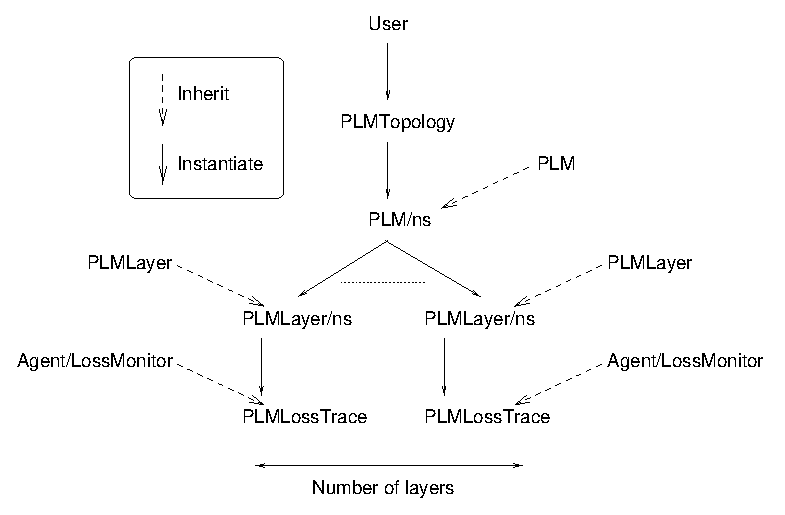
\includegraphics{figures/instanPLMrecv.eps}}
  \caption{Inheritance and instantiation when we create a receiver.}
  \label{fig:instanPLMrecv}
\end{figure}

All the PLM machinery is implemented at the receiver. In this section we decribe
the instantiation process of a receiver. To create, place at node
{\tt n},  attach to source {\tt S}, and start at {\tt t$_1$} a PLM receiver we
call the PLMTopology instproc {\tt 
  build\_receiver n addr t$_1$ C} where {\tt addr} is the address returned
by {\tt place\_source} when {\tt S} was created, and {\tt C} is the check value. The
receiver created by {\tt build\_receiver} is an instance of the class PLM/ns,
the ns interface to the PLM 
machinery. At the initialisation of the receiver, the PLM instproc {\tt init} is
called due to inheritance. {\tt init} calls the PLM/ns instproc
{\tt create-layer} and, by this way,  creates as many instances of the class 
PLMLayer/ns (the ns interface to the PLMLayer class) as there are layers. Each
instance of PLMLayer/ns creates an instance of the class PLMLossTrace which is
reponsible for 
monitoring the received and lost packets thanks to the fact that the class
PLMLossTrace inherits from the class LossMonitor. 
Fig.~\ref{fig:instanPLMrecv} schematically describes the process  of a PLM
receiver instantiation. In the following we describe the behavior of a PLM
receiver when it receives a packet and when it detects a loss.



\subsection{Reception of a Packet}
\label{sec:PLMReception-Packet}
We add in {\tt void LossMonitor::recv(Packet* pkt, Handler*)} a Tcl call to the
  LossMonitor instproc {\tt log-PP} each time a packet is received :
\begin{program}
  void LossMonitor::recv(Packet* pkt, Handler*)
  {
    ...
    if (expected_ >= 0) {
      ...
      }
    Tcl::instance().evalf("%s log-PP", name());
    }
\end{program}

The LossMonitor instproc {\tt log-PP} is empty. In fact, we define the {\tt
  log-PP} instproc for the class PLMLossTrace. {\tt log-PP}
computes an estimate of the available bandwidth based on a single PP burst (of
length {\tt PP\_burst\_length} in packets). Once {\tt log-PP} has received the 
  {\tt PP\_burst\_length} packets of the burst, it computes the estimate and
  calls the PLM instproc {\tt make\_estimate} with the computed estimate as
  argument. 

{\tt make\_estimate} puts the estimate based on a single PP
({\tt PP\_value}) in an array of  estimate samples ({\tt PP\_estimate}). If {\tt
  PP\_value} is lower than the current subscription level (i.e.~lower than the
throughput achieved according to the current number of layers subscribed), {\tt
  make\_estimate} calls the PLM instproc {\tt stability-drop} which simply drops
layers until the current subscription level becomes lower than {\tt PP\_value}.
{\tt make\_estimate} makes an estimate {\tt PP\_estimate\_value} by taking the
minimum {\tt PP\_value} received during the last {\tt check\_estimate} period
(if there are at
least {\tt PP\_estimation\_length} single PP estimate received). Once {\tt
  make\_estimate} has a {\tt PP\_estimate\_value} it calls the PLM instproc {\tt
  choose\_layer} which joins or drops layer(s) according to the current subscription
level and to the {\tt PP\_estimate\_value}. For details about the PLM instproc
\code{make_estimate}, refer to its code in \nsf{tcl/plm/plm.tcl}.



\subsection{Detection of a Loss}
Each time a loss is detected by an instance of the class LossMonitor, a call to
the LossMonitor instproc {\tt log-loss} is triggered. The LossMonitor instproc {\tt log-loss}
is empty. In fact, we define the {\tt log-loss} instproc for the class
PLMLossTrace. The PLMLossTrace instproc {\tt log-loss} simply
calls the PLM instproc {\tt log-loss} which contains the PLM machinery in case
of loss. In summary, {\tt log-loss} only drops a layer when the loss rate
exceeds 10\% (this test is executed by the PLM instproc {\tt
  exeed\_loss\_thresh}). After a layer drop {\tt log-loss} precludes any
other layer drop due to loss for 500ms. For details about the PLM instproc {\tt
  log-loss}, refer to its code in \nsf{tcl/plm/plm.tcl}. 

\subsection{Joining or Leaving a Layer}
To join a layer the PLM instproc {\tt add-layer} is called. This instproc
calls the PLMLayer instproc {\tt join-group} which calls the PLMLayer/ns instproc {\tt
  join-group}.
To leave a layer the PLM instproc {\tt drop-layer} is called. This instproc
calls the PLMLayer instproc {\tt leave-group} which calls the PLMLayer/ns instproc {\tt
  leave-group}.

\section{Commands at a Glance}
Note: This section is a copy paste of the end of
section~\ref{sec:Configuration}. We add this section to preserve homogeneity with
the ns manual.

All the simulations for PLM should be set using the PLMTopology environment (as
in the example script where we define a PLMTopology superclass called Scenario0). The
user interface is (all the instproc can be found in \nsf{tcl/plm/plm-topo.tcl}):
\begin{description}
\item[\tt build\_link a b d bw] creates a duplex link between node
  \code{a} and \code{b} with a delay \code{d} and a bandwidth \code{bw}. If
  either node does not exist, \code{build_link} creates it.
\item[\tt place\_source n t] creates and places a PLM source at node \code{n} and
  starts it at time \code{t}. \code{place_source} returns \code{addr} which
  allows to attach receivers to this source.
\item[\tt place\_receiver n addr C nb] creates and places a PLM receiver at node
  \code{n} and attached it to the source which return the address \code{addr}. The
  check value for this PLM receiver is \code{C}. An optional parameter \code{nb}
  allows to get an instance of the PLM receiver called \code{PLMrcvr($nb)}. This
  instance is only useful to get some specific statistics about this receiver
  (mainly the number of packets received or lost). %$
\end{description}
}

% Local Variables: 
% mode: latex
% TeX-master: t
% End: 


\part{Application}
\chapter{Applications and transport agent API}
\label{chap:applications}

In \ns, applications sit on top of transport agents.  There are two basic types
of applications:  sources and traffic generators.  Generally, source objects
are used to generate traffic that is transported by TCP Agent objects, and
traffic generators are used in conjunction with UDP Agent objects.  
Figure~\ref{fig:application} illustrates two examples of how applications
are composed and attached to transport agents.  Transport agents are described
in Part V (Transport).

\begin{figure}[tb] 
  \centerline{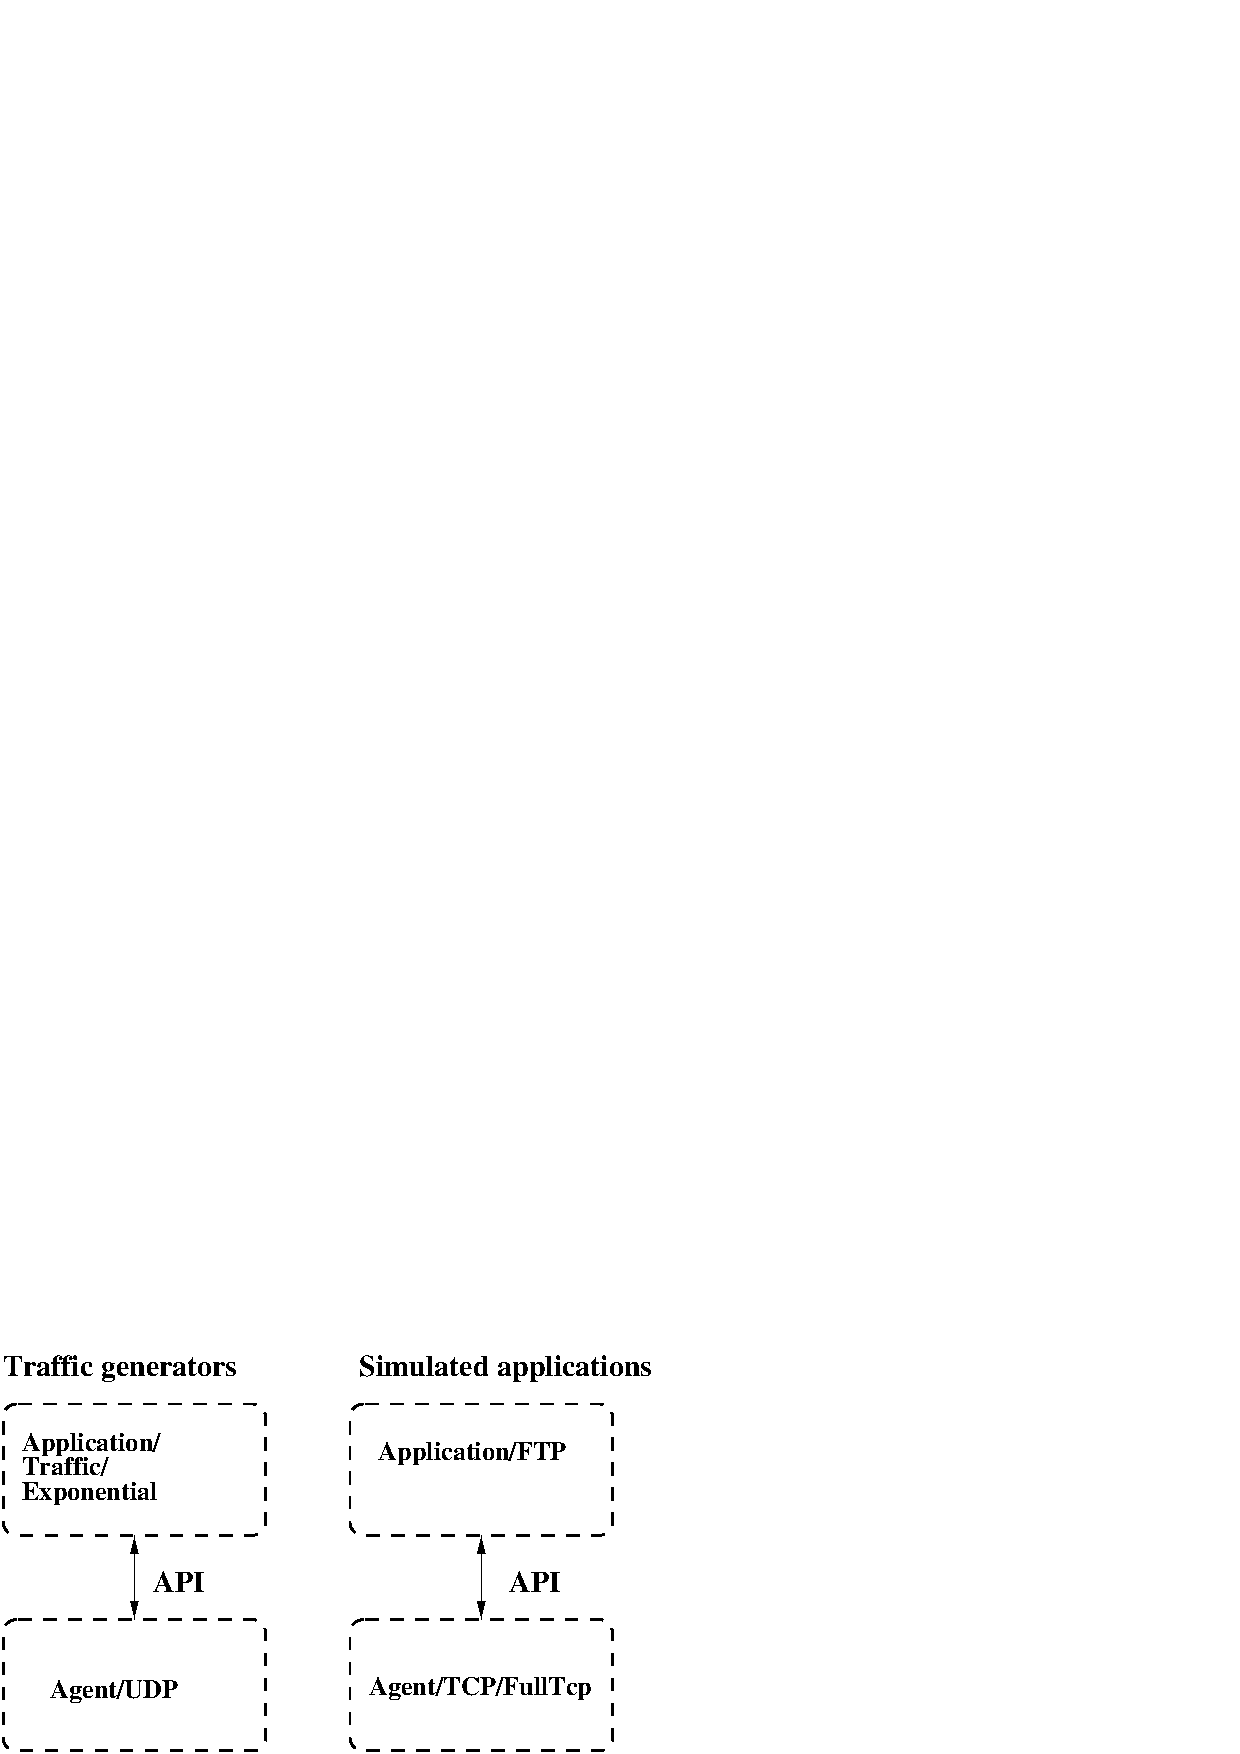
\includegraphics{application}}
  \caption{Example of Application Composition}
  \label{fig:application} 
\end{figure}

This chapter first describes the base \clsref{Application}{../ns-2/app.h}. 
Next, the transport API, through which applications request services from
underlying transport agents, is described.  Finally, the current 
implementations of traffic generators and sources are explained.  

%There are currently two methods of traffic generation in \ns.
%One method uses the abstract
%\clsref{TrafficGenerator}{../ns-2/trafgen.h}
%to generate inter-packet intervals and packet sizes.
%Currently, classes derived
%from TrafficGenerator are used in conjunction with the UDP\_Agent
%objects, which are responsible for actually allocating and
%transmitting the generated packets (Section~\ref{sec:trafgenclass}).
%The second method of traffic generation uses the Source class.
%Source objects generate traffic that is transported by TCPAgent objects
%(Section~\ref{sec:sourceobjects}).

\section{The class Application}
\label{sec:appclass}

Application is a C++ class defined as follows:
\begin{program}
        class Application : public TclObject \{
        public:
                Application();
                virtual void send(int nbytes);
                virtual void recv(int nbytes);
                virtual void resume();
        protected:
                int command(int argc, const char*const* argv);
                virtual void start();
                virtual void stop();
                Agent *agent_;
                int enableRecv_;                // call OTcl recv or not
                int enableResume_;              // call OTcl resume or not
        \};
\end{program}
Although objects of \code{class Application} are not meant to be instantiated,
we do not make it an abstract base class so that it is visible from OTcl level.
The class provides basic prototypes for application behavior 
(\code{send(), recv(), resume(), start(), stop()}), a pointer to the 
transport agent to which it is connected, and flags that indicate whether
a OTcl-level upcall should be made for \code{recv()} and 
\code{resume()} events.  

\section{The transport agent API}
In real-world systems, applications typically access network services through
a well-defined applications programming interface (API).  The most popular
of these APIs is known as ``sockets.''  In \ns, we mimic the behavior of the
sockets API through a set of well-defined API functions.  These functions 
are then mapped to the appropriate internal agent functions (e.g.,
a call to \code{send(numBytes)} causes TCP to increment its ``send buffer'' 
by a corresponding number of bytes).

This section describes how agents and applications are hooked together and
communicate with one another via the API.

\subsection{Attaching transport agents to nodes}
\label{sec:attachagentnode}
This step is typically done at OTcl level.  Agent management was also briefly
discussed in Section \ref{sec:node:node}.  

\begin{program}
        set src [new Agent/TCP/FullTcp]
        set sink [new Agent/TCP/FullTcp]
        $ns_ attach-agent $node_(s1) $src
        $ns_ attach-agent $node_(k1) $sink
        $ns_ connect $src $sink
\end{program}

The above code illustrates that in \ns, agents are first attached to a node
via \code{attach-agent}.  Next, the \code{connect} instproc sets each agent's
destination target to the other.  Note that, in \ns, \code{connect()} has
different semantics than in regular sockets.  In \ns, \code{connect()} simply
establishes the destination address for an agent, but does not set up the
connection.  As a result, the overlying application does not need to know
its peer's address.  For TCPs that exchange SYN segments, the first call to 
\code{send()} will trigger the SYN exchange. 

To detach an agent from a node, the instproc \code{detach-agent} can be 
used; this resets the target for the agent to a null agent.

\subsection{Using transport agents via system calls}
\label{sec:systemcalls}
Once transport agents have been configured, applications can use their 
services via the following system calls.  These calls can be invoked at either
OTcl or C++ level, thereby allowing applications to be coded in either C++ or
OTcl.  These functions have been implemented as virtual functions in the base
\code{class Agent}, and can be redefined as needed by derived Agents. 
\begin{itemize}
\item \code{send(int nbytes)}---Send nbytes of data to peer.  For TCP agents,
if \code{nbytes == -1}, this corresponds to an ``infinite'' send; i.e., the
TCP agent will act as if its send buffer is continually replenished by the
application.
\item \code{sendmsg(int nbytes, const char* flags = 0)}---Identical to 
\code{send(int nbytes)}, except that it passes an additional string 
\code{flags}.  Currently one flag value, ``MSG\_EOF,'' is defined; MSG\_EOF
specifies that this is the last batch of data that the application will 
submit, and serves as an implied close (so that TCP can send FIN with data).
\item \code{close()}---Requests the agent to close the connection (only 
applicable for TCP).
\item \code{listen()}---Requests the agent to listen for new connections
(only applicable for Full TCP).
\end{itemize}
Note that certain calls are not applicable for certain agents; e.g., a call
to \fcn[]{close} a UDP connection results in a no-op.  Additional calls
can be implemented in specialized agents, provided that they are made
\code{public} member functions. 

\subsection{Attaching applications to agents}
\label{sec:attachappagent}

After applications are instantiated, they must be connected to a transport
agent.  The \code{attach-agent} method can be used to attach an application
to an agent, as follows:
\begin{program}
        set ftp1 [new Application/FTP]
        $ftp1 attach-agent $src
\end{program}

The attach-agent method is implemented in C++.  It sets the \code{agent_}
pointer in \code{class Application} to point to the transport agent, and then
it calls \code{attachApp()} in \code{agent.cc} to set the \code{app_} pointer
to point back to the application.  By maintaining this binding only in C++,
OTcl-level instvars pointers are avoided and consistency between OTcl and C++ 
is guaranteed.  The OTcl-level command \code{[$ftp1 agent]} can be used by 
applications to obtain the handler for the transport agent.

\subsection{Upcalls to applications}
\label{sec:upcalls}

Since presently in \ns there is no actual data being passed between 
applications, agents can instead announce to applications the occurence of 
certain events at the transport layer through ``upcalls.''  For example,
applications can be notified of the arrival of a number of bytes of data;
this information may aid the application in modelling real-world application
behavior more closely.  Two basic ``upcalls'' have been implemented in 
base \code{class Application}:
\begin{itemize} 
\item \code{recv(int nbytes)}---Announces that \code{nbytes} of data have been
received by the agent.  For UDP agents, this signifies the arrival of
a single packet.  For TCP agents, this signifies the ``delivery'' of an 
amount of in-sequence data, but does not necessarily correspond with the 
arrival of a certain number of packets (due to the possibility of reordering
in the network).
\item \code{resume()}---This indicates to the application that the transport
agent has sent out all of the data submitted to it up to that point in time.  
For TCP, it does not indicate whether the data has been ACKed yet, only that
it has been sent out for the first time. 
\end{itemize}
The default behavior is as follows: 
If an application has been implemented at OTcl-level, these C++ functions
call a similarly named (\code{recv, resume}) OTcl method in the application,
if such methods have been defined.   

Although strictly not a callback to applications, certain Agents have
implemented a callback from C++ to OTcl-level that has been used by 
applications such as HTTP simulators.  This callback method, \code{done()},
is used in TCP and CBR agents\footnote{CBR agents are a combination of UDP 
agent and CBR traffic generator that was implemented before this API was 
finalized.  Under the current API structure, CBR traffic generators can be
implemented as \code{class Application/Traffic/CBR} on top of a UDP agent}.
In TCP, \code{done} is called when a TCP sender has received ACKs for all of 
its data and is now closed.  In CBR agents, \code{done} indicates that
the CBR agent has stopped, due to either a user request or a lack of 
packets to send.

\subsection{An example}
\label{sec:syscallsexample}
Here is an example of how the API is used to implement a simple application
(FTP) on top of a FullTCP connection. 

\begin{program}
        set src [new Agent/TCP/FullTcp]
        set sink [new Agent/TCP/FullTcp]
        $ns_ attach-agent $node_(s1) $src
        $ns_ attach-agent $node_(k1) $sink
        $ns_ connect $src $sink

        # set up TCP-level connections
        $sink listen; 
        $src set window_ 100

        set ftp1 [new Application/FTP]
        $ftp1 attach-agent $src

        $ns_ at 0.0 "$ftp1 start"
\end{program}

In the configuration script, the first five lines of code allocates two new
FullTcp agents, attaches them to the correct nodes, and "connects" them
together (assigns the correct destination addresses to each agent).  The
next two lines configure the TCP agents further, placing one of them in
LISTEN mode.  Next, \code{ftp1} is defined as a new FTP Application, and 
the \code{attach-agent} method is called in C++ (\code{app.cc}).     

The ftp1 application is started at time 0:
\begin{program}
        Application/FTP instproc start \{\} \{
      	        [$self agent] send -1;   # Send indefinitely
        \}
\end{program}
Alternatively, the FTP application could have been implemented in C++ as
follows:
\begin{program}
        void FTP::start()
        \{
                agent_->send(-1);    // Send indefinitely
        \}
\end{program}  
Since the FTP application does not make use of callbacks, these functions
are null in C++ and no OTcl callbacks are made. 

\section{The class TrafficGenerator}
\label{sec:trafgenclass}

TrafficGenerator is an abstract C++ class defined as follows:
\begin{program}
        class TrafficGenerator : public Application \{
        public:
                TrafficGenerator();
                virtual double next_interval(int &) = 0;
                virtual void init() \{\}
                virtual double interval() \{ return 0; \}
                virtual int on() \{ return 0; \}
                virtual void timeout();
                virtual void recv() \{\}
                virtual void resume() \{\}
        protected:
                virtual void start();
                virtual void stop();
                double nextPkttime_;
                int size_;
                int running_;
                TrafficTimer timer_;
        \};
\end{program}
The pure virtual function \fcn[]{next\_interval} returns the time until the
next packet is created and also sets the size in bytes of the next
packet.  The function \fcn[]{start} calls \fcn{init} and starts the 
timer.  The function \fcn[]{timeout} sends a packet and reschedules the
next timeout.  The function \fcn[]{stop} cancels any pending transmissions.
Callbacks are typically not used for traffic generators, so these 
functions (\code{recv, resume}) are null.

Currently, there are four C++ classes derived from the
class TrafficGenerator:
\begin{enumerate}
\item \code{EXPOO_Source}---generates traffic according to an
  Exponential On/Off distribution.
  Packets are sent at a fixed rate during on periods, and
  no packets are sent during off periods.
  Both on and off periods are taken from an exponential distribution.
  Packets are constant size.
\item \code{POO_Source}---generates traffic
  according to a Pareto On/Off distribution.
  This is identical to the Exponential On/Off distribution,
  except the on and off periods are taken from a pareto distribution.
  These sources can be used to generate aggregate traffic
  that exhibits long range dependency.
\item \code{CBR_Source}---generates traffic according to a deterministic rate.
  Packets are constant size.  Optionally, some randomizing dither can be
  enabled on the interpacket departure intervals. 
\item \code{TrafficTrace}---generates traffic according to a trace file.
  Each record in the trace file consists of 2 32-bit fields.
  The first contains the time in microseconds
  until the next packet is generated.
  The second contains the length in bytes of the next packet.
\end{enumerate}
These classes can be created from OTcl.  The OTcl classes names and
associated parameters are given below:

\paragraph{Exponential On/Off}
An Exponential On/Off object is embodied in the OTcl class
Application/Traffic/Expoo.  The member variables that parameterize this
object are:
\begin{alist}
\code{packet-size} & the constant size of the packets generated\\
\code{burst-time} & the average "on" time for the source\\
\code{idle-time} & the average "off" time for the source\\
\code{rate} & the sending rate during "on" times\\
\end{alist}
Hence a new Exponential On/Off source can be created and parameterized
as follows:
\begin{program}
        set e [new Application/Traffic/Expoo]
        $e set packet-size 210
        $e set burst-time 500ms
        $e set idle-time 500ms
        $e set rate 100k
\end{program}

\paragraph{Pareto On/Off}
A Pareto On/Off object is embodied in the OTcl class Application/Traffic/Pareto.
The member variables that parameterize this object are:
\begin{alist}
\code{packet-size} & the constant size of the packets generated\\
\code{burst-time} & the average "on" time for the source\\
\code{idle-time} & the average "off" time for the source\\
\code{rate} & the sending rate during "on" times\\
\code{shape} & the "shape" parameter used by the pareto distribution\\
\end{alist}
A new Pareto On/Off source can be created as follows:
\begin{program}
        set p [new Application/Traffic/Pareto]
        $p set packet-size 210
        $p set burst-time 500ms
        $p set idle-time 500ms
        $p set rate 200k
        $p set shape 1.5
\end{program}

\paragraph{CBR}
A CBR  object is embodied in the OTcl class
Application/Traffic/CBR.  The member variables that parameterize this
object are:  
\begin{alist}
\code{rate} & the sending rate \\
\code{packet-size} & the constant size of the packets generated\\
\code{random} & flag indicating whether or not to introduce random ``noise'' 
in the scheduled departure times (default is off)\\
\end{alist}
Hence a new CBR source can be created and parameterized
as follows:
\begin{program}
        set e [new Application/Traffic/CBR]
        $e set packet-size 48
        $e set rate 64Kb
        $e set random 1
\end{program}

\paragraph{Traffic Trace}
A Traffic Trace object is instantiated by the OTcl class 
Application/Traffic/Trace.
The associated class Tracefile is used to enable multiple 
Traffic/Trace objects to be associated with a single trace file.
The Traffic/Trace class uses the method attach-tracefile to associate
a Traffic/Trace object with a particular Tracefile object.
The method filename of the Tracefile class associates a trace file
with the Tracefile object.
The following example shows how to create two Application/Traffic/Trace objects,
each associated with the same trace file
(called "example-trace" in this example).
To avoid synchronization of the traffic generated,
random starting places within the trace file are chosen for
each Traffic/Trace object.
\begin{program}
        set tfile [new Tracefile]
        $tfile filename example-trace

        set t1 [new Application/Traffic/Trace]
        $t1 attach-tracefile $tfile
        set t2 [new Application/Traffic/Trace]
        $t2 attach-tracefile $tfile
\end{program}

\subsection{An example}

The following code illustrates the basic steps to configure an Exponential
traffic source over a UDP agent, for traffic flowing from node s1 to node k1:

\begin{program}
        set src [new Agent/UDP]
        set sink [new Agent/UDP]
        $ns_ attach-agent $node_(s1) $src
        $ns_ attach-agent $node_(k1) $sink
        $ns_ connect $src $sink
	
        set e [new Application/Traffic/Expoo]
        $e attach-agent $src
        $e set packet-size 210
        $e set burst-time 500ms
        $e set idle-time 500ms
        $e set rate 100k

        $ns_ at 0.0 "$e start"
\end{program}

\section{Simulated applications}
\label{sec:simapps}
 
There are currently two ``application'' classes derived from Application:
Application/FTP and Application/Telnet.  These classes work by advancing the
count of packets available to be sent by a TCP transport agent.
The actual transmission of available packets is still controlled by TCP's flow 
control algorithm.
 
\paragraph{Application/FTP} 
Application/FTP, implemented in OTcl, simulates bulk data transfer.  
The following are methods of the Application/FTP class:
\begin{alist}
\code{attach-agent} & attaches an Application/FTP object to an agent.\\ 
\code{start} & start the Application/FTP by calling the TCP agent's 
\code{send(-1)} function, which causes TCP to behave as if the application 
were continuously sending new data.\\
\code{stop} & stop sending.\\ 
\code{produce n} &  set the counter of packets to be sent to $n$.\\ 
\code{producemore n} &  increase the counter of packets to be sent by $n$. \\
\code{send n} & similar to \code{producemore}, but sends $n$ bytes instead of
packets.  
\end{alist} 

\paragraph{Application/Telnet} 
Application/Telnet objects generate packets in one of two ways.
If the member variable \code{interval_} is non-zero,
then inter-packet times are chosen
from an exponential distribution with average equal to \code{interval_}.
If \code{interval_} is zero, then inter-arrival times are chosen
according to the tcplib distribution (see tcplib-telnet.cc).
The start method starts the packet generation process.
 
\endinput

\chapter{Web cache as an application}
\label{chap:webcache}

All applications described above are ``virtual'' applications, in the sense
that they do not actually transfer their own data in the simulator; all 
that matter is the \emph{size} and the \emph{time} when data are transferred.
Sometimes we may want applications to transfer their own data in simulations.
One such example is web caching, where we want HTTP servers to send HTTP 
headers to caches and clients. These headers contain 
page modification time information and other caching directives, which are 
important for some cache consistency algorithms.

In the following, we first describe general issues regarding
transmitting application-level data in \ns, then we discuss special
issues, as well as APIs, related to transmitting application data
using TCP as transport. We will then proceed to discuss the internal
design of HTTP client, server, and proxy cache. 

\section{Using application-level data in \ns}

\begin{figure}[tb]
  \begin{center}
    \centerline{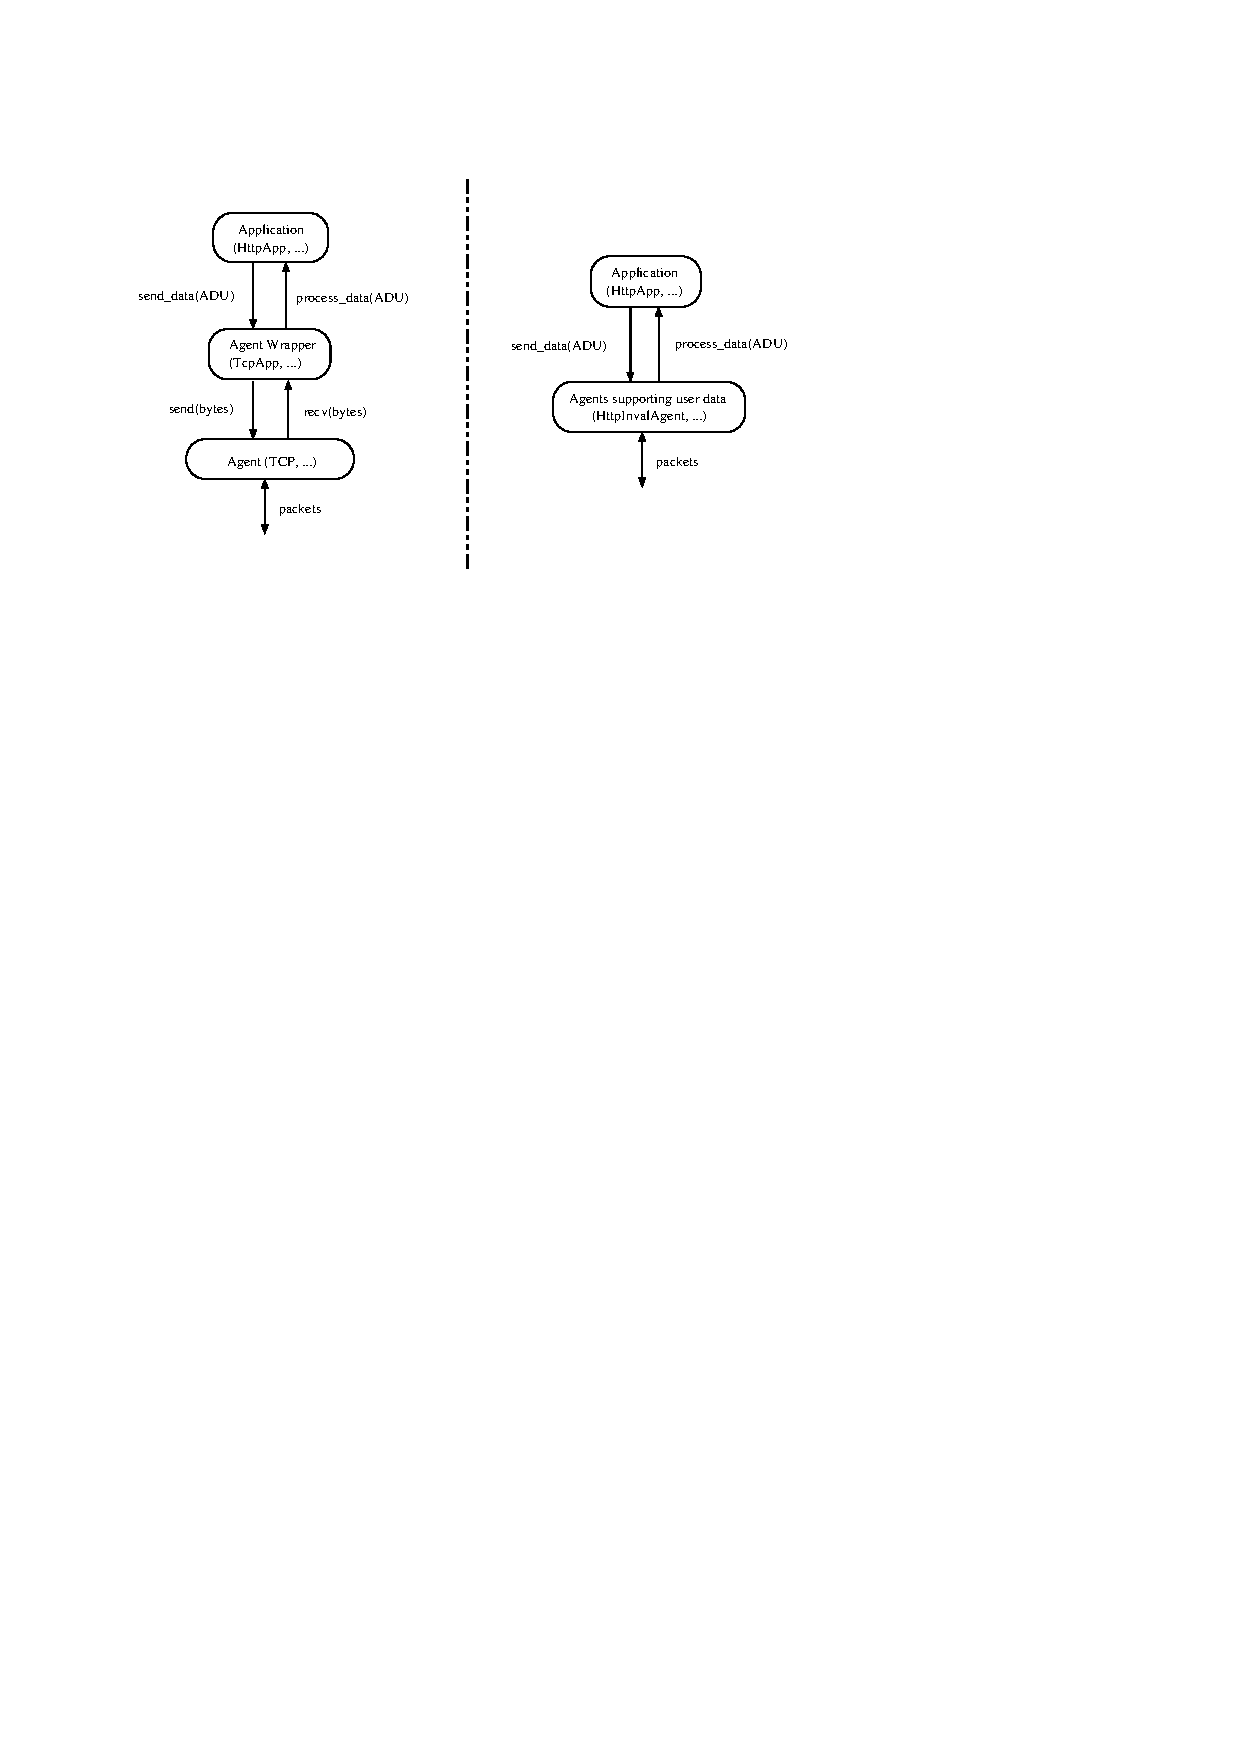
\includegraphics{app-dataflow}}
    \caption{Examples of application-level data flow}
    \label{fig:app-dataflow}
  \end{center}
\end{figure}

In order to transmit application-level data in \ns, we provide a 
uniform structure to pass data among applications, and to
pass data from applications to transport agents (Figure
\ref{fig:app-dataflow}). It has three major components: 
a representation of a uniform application-level data unit (ADU), a 
common interface to pass data between applications, and two mechanisms
to pass data between applications and transport agents.

\subsection{ADU} 

The functionality of an ADU is similar to that of a Packet. It needs to
pack user data into an array, which is then included in the user data
area of an \ns packet by an Agent (this is not supported by current
Agents. User must derive new agents to accept user data from
applications, or use an wrapper like TcpApp. We'll discuss this
later). 

Compared with Packet, ADU provides this functionality in a different
way. In Packet, a common area is allocated for all packet headers; an
offset is used to access different headers in this area. In ADU this
is not applicable, because some ADU allocates their space dynamically
according the the availability of user data. For example, if we want
to deliver an OTcl script between applications, the size of the script
is undetermined beforehand. Therefore, we choose a less efficient but
more flexible method. Each ADU defines its own data members, and
provides methods to serialize them (i.e., pack data into an array and
extract them from an array). For example, in the abstract base class
of all ADU, AppData, we have:

\begin{program}
        class AppData \{
        private:
                AppDataType type_;  // ADU type
        public:
                struct hdr \{
                        AppDataType type_;
                \};
        public:
                AppData(char* b) \{
                        assert(b != NULL);
                        type_ = ((hdr *)b)->type_;
                \}
                virtual void pack(char* buf) const;
        \}
\end{program}

Here \code{pack(char* buf)} is used to write an AppData object
into an array, and \code{AppData(char* b)} is used to build a new
AppData from a ``serialized'' copy of the object in an array.

When deriving new ADU from the base class, users may add more data,
but at the same time a new \code{pack(char *b)} and a new constructor 
should be provided to write and read those new data members from an
array. For an example as how to derive from an ADU, look at 
\ns/webcache/http-aux.h.

\subsection{Passing data between applications}

The class Application does not define how to handle application-level
data, nor does it define how to pass those data between
applications. We provide an abstract interface, class AppConnector,
for this purpose. It's defined as follows:

\begin{program}
        class AppConnector \{
        public: 
                AppConnector() : target_(0) \{\}
                inline AppConnector*& target() \{ return target_; \}

                virtual void process_data(int size, char* data) = 0;
                virtual void send_data(int size, char* data = 0);

        protected:
                AppConnector* target_;
        \};
\end{program}

AppConnector enables Applications to link together, just as Connector
enables Agents to link together. An application can either inherit
directly from AppConnector, or it can inherit from both TclObject (or
another Application) and AppConnector. The latter allows an
application to both handle user data and to enjoy the benefits
provided by TclCL (e.g., split object). For example, in the web cache
code, class HttpApp is derived from both TclObject and AppConnector 
(\ns/webcache/http.h), and class TcpApp is derived from both
AppConnector and Application. 

\subsection{Transmitting user data over UDP}

Currently there are no supports in class Agent to transmit user
data. There are two ways to  transmit serialized ADU through transport
agents. First, for UDP agent (and all agents derived from there), we
can derive from class UDP and add a new method
\code{send(int nbytes, char *userdata)} to pass user data from
Application to Agent. To pass data from an Agent to an Application is
somewhat trickier: each agent has a pointer to its attached
application, we dynamically cast this pointer to an AppConnector and
then call \code{AppConnector::process_data()}.

As an example, we illustrate how class HttpInvalAgent is
implemented. It is based on UDP, and is inteded to deliver web cache
invalidation messages (\ns/webcache/inval-agent.h). It is defined as:

\begin{program}
        class HttpInvalAgent : public Agent \{
        public: 
                HttpInvalAgent();

                virtual void recv(Packet *, Handler *);
                virtual void send(int realsize, AppData* data);

        protected:
                int off_inv_;
        \};
\end{program}

Here \code{recv(Packet*, Handler*)} overridden to extract user data,
and a new \code{send(int, AppData*)} is provided to include user data
in packetes. An application (HttpApp) is attached to an HttpInvalAgent
using \code{Agent::attachApp()} (a dynamic cast is needed). In
\code{send()}, the following code is used to write user data from
AppData to the user data area in a packet:

\begin{program}
        Packet *pkt = allocpkt(data->size());
        hdr_inval *ih = (hdr_inval *)pkt->access(off_inv_);
        ih->size() = data->size();
        char *p = (char *)pkt->accessdata();
        data->pack(p);
\end{program}

In \code{recv()}, the following code is used to read user data from
packet and to deliver to the attached application:

\begin{program}
        hdr_inval *ih = (hdr_inval *)pkt->access(off_inv_);
        ((HttpApp*)app_)->process_data(ih->size(), (char *)pkt->accessdata());
        Packet::free(pkt);
\end{program}


\subsection{Transmitting user data over TCP}
\label{sec:webcache-tcpapp}

Transmitting user data using TCP is trickier than doing that over UDP,
mainly because of TCP's reassembly queue is only available for
FullTcp. We deal with this problem by abstracting a TCP connection as
a FIFO pipe. 

As indicated in section \ref{sec:upcalls}, transmission of application data
can be implemented via agent upcalls. Assuming we are using TCP agents, 
all data are delivered in sequence, which means we can view the TCP 
connection as a FIFO pipe. We emulate user data transmission over TCP
as follows. We first provide buffer 
for application data at the sender. Then we count the bytes received at the 
receiver. When the receiver has got all bytes of the current data transmission,
it then gets the data directly from the sender. Class Application/TcpApp is 
used to implement this functionality.

A TcpApp object contains a pointer to a transport agent, presumably either
a FullTcp or a SimpleTcp.
\footnote{A SimpleTcp agent is used solely for web caching simulations. It 
is actually an UDP agent. It has neither error recovery nor flow/congestion
control. It doesn't do packet segmentation. Assuming a loss-free network 
and in-order packet delivery,
SimpleTcp agent simplifies the trace files 
and hence aids the debugging of application protocols, which, in our case, 
is the web cache consistency protocol.}
(Currently TcpApp doesn't support asymmetric TCP agents, i.e., sender is
separated from receiver). It provides the following OTcl interfaces:

\begin{itemize}
\item \code{connect}: Connecting another TcpApp to this one. This
  connection is bi-directional, i.e., only one call to \code{connect} is 
  needed, and data can be sent in either direction. 
\item \code{send}: It takes two arguments: \code{(nbytes, str)}.
  \code{nbytes} is the ``nominal'' size of application data. \code{str} 
  is application data in string form.
\end{itemize}

In order to send application data in binary form, TcpApp provides a 
virtual C++ method \code{send(int nbytes, int dsize, const char *data)}.
In fact, this is the method used to implement the OTcl method \code{send}.
Because it's difficult to deal with binary data in Tcl, no OTcl interface
is provided to handle binary data. \code{nbytes} is the number of bytes 
to be transmitted, \code{dsize} is the actual size of the array \code{data}.

TcpApp provides a C++ virtual method \code{process_data(int size, char*data)}
to handle the received data. The default handling is to treat the data 
as a tcl script and evaluate the script. But it's easy to derive a class
to provide other types of handling.

Here is an example of using Application/TcpApp. A similar example is 
\code{Test/TcpApp-2node} in \ns/tcl/test/test-suite-webcache.tcl.
First, we create FullTcp agents and connect them:

\begin{program}
        set tcp1 [new Agent/TCP/FullTcp]
        set tcp2 [new Agent/TCP/FullTcp]
        # {\cf Set TCP parameters here, e.g., window_, iss_, \ldots}

        $ns attach-agent $n1 $tcp1
        $ns attach-agent $n2 $tcp2
        $ns connect $tcp1 $tcp2
        $tcp2 listen
\end{program}

Then we Create TcpApps and connect them:

\begin{program}
        set app1 [new Application/TcpApp $tcp1]
        set app2 [new Application/TcpApp $tcp2]
        $app1 connect $app2
\end{program}

Now we let \code{$app1} %$
be sender and \code{$app2} %$ 
be receiver:

\begin{program}
        $ns at 1.0 "$app1 send 100 \bs"$app2 app-recv 100\bs""
\end{program} %$

Where \code{app-recv} is defined as:

\begin{program}
        Application/TcpApp instproc app-recv { size } {
                global ns
                puts "[$ns now] app2 receives data $size from app1"
        }
\end{program}

\subsection{Class hierarchy related to user data handling}

We conclude this section by providing a hierarchy of classes involved
in this section (Figure \ref{fig:appdata-hier}).

\begin{figure}[tb]
  \begin{center}
    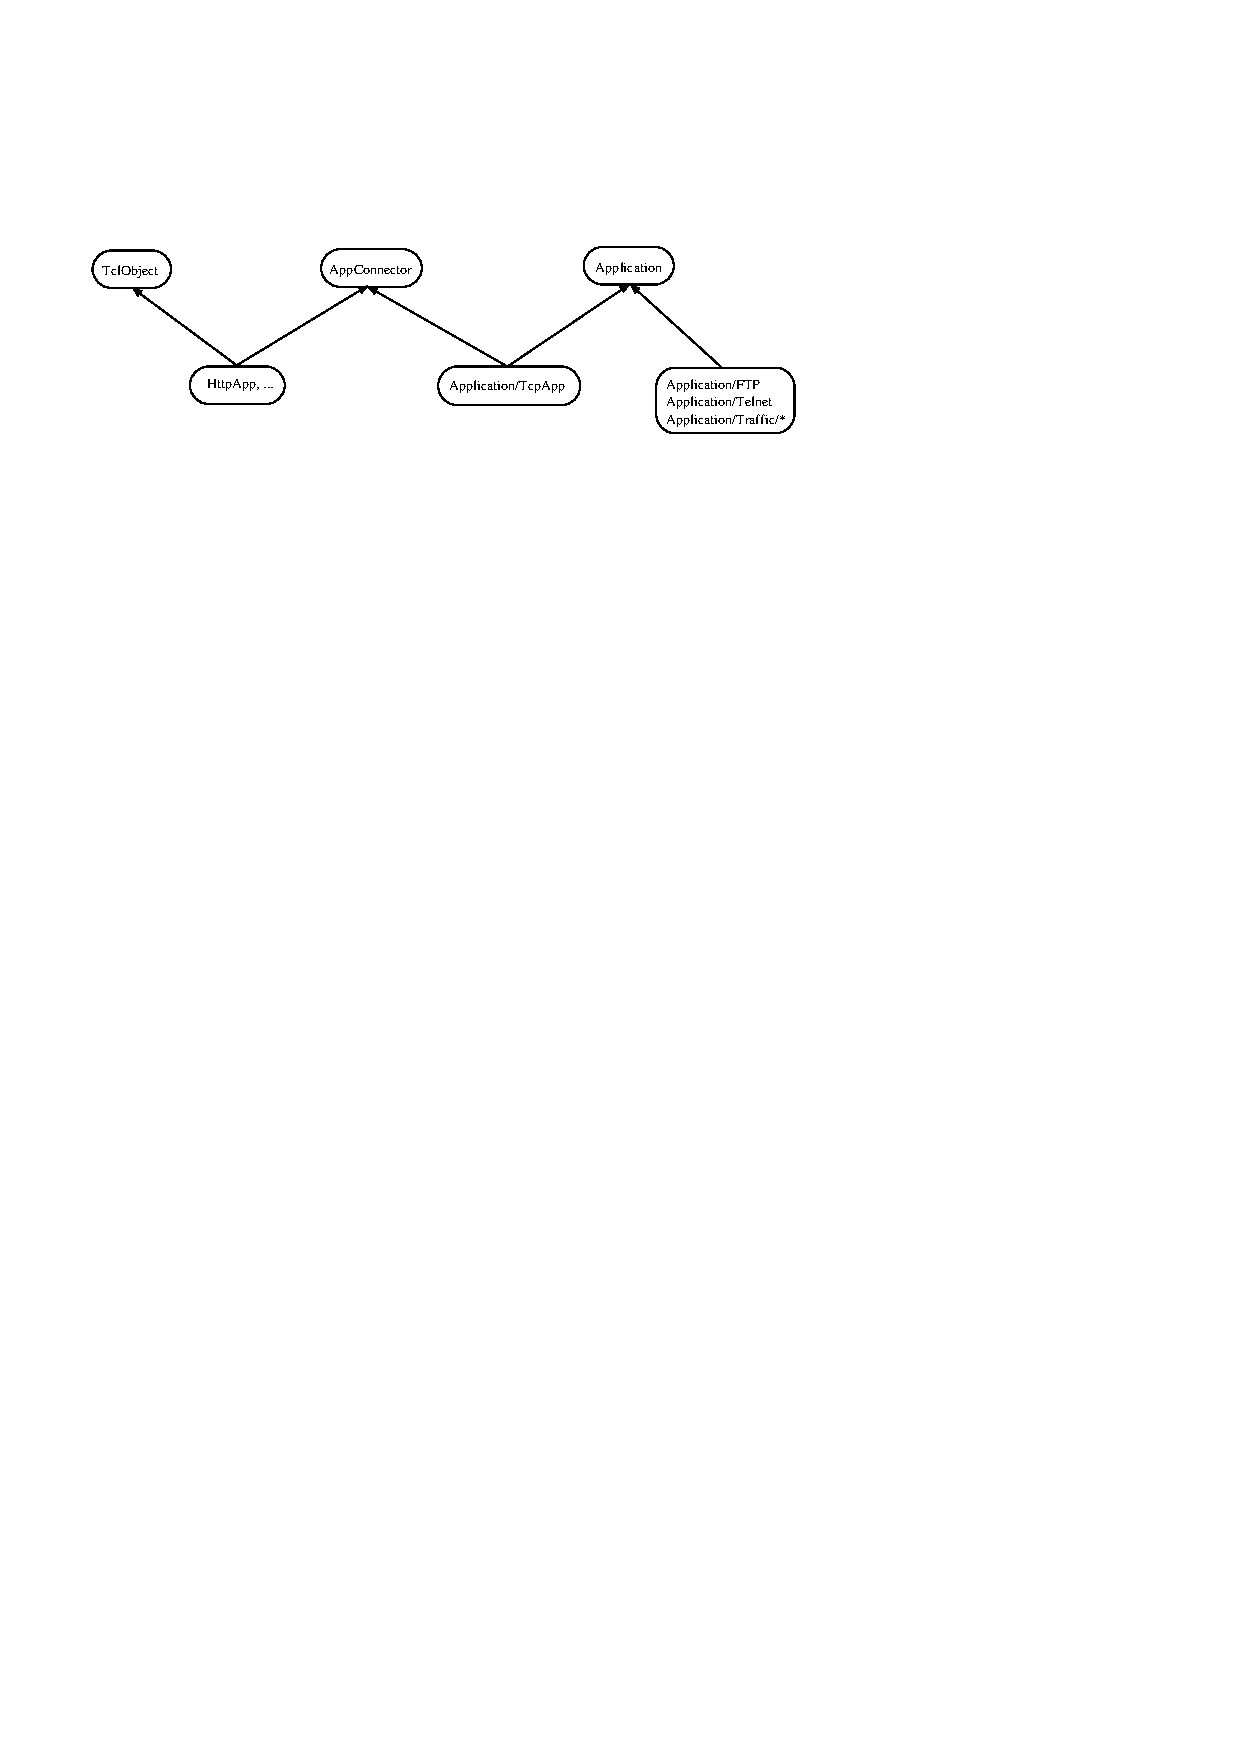
\includegraphics{appdata-hier}
    \caption{Hierarchy of classes related to application-level data handling}
    \label{fig:appdata-hier}
  \end{center}
\end{figure}


\section{Overview of web cache classes}
\label{sec:webcache-class}

There are three major classes related to web cache, as it is in the
real world: client (browser), server, and cache. Because they share a
common feature, i.e., the HTTP protocol, they are derived from the
same base class \code{Http} (Name of OTcl class, it's called
\code{HttpApp} in C++). For the following reasons, it's not a real
Application.  First, an HTTP object (i.e., client/cache/server) may
want to maintain multiple concurrent HTTP connections, but an
Application contains only one \code{agent_}.  Also, an HTTP object
needs to transmit real data (e.g., HTTP header) and that's provided by
TcpApp instead of any Agent. Therefore, we choose to use a standalone
class derived from TclObject for common features of all HTTP objects,
which are managing HTTP connections and a set of pages.  In the rest
of the section, we'll discuss these functionalities of Http. In the
next three sections, we'll in turn describe HTTP client, cache and
server.

\subsection{Managing HTTP connections}
\label{sec:webcache-connection}

Every HTTP connection is embodied as a TcpApp
object. Http maintains a hash of TcpApp objects, which are all of 
its active connections. It assumes that to any other Http, it 
has only one HTTP connection. It also allows dynamic establishment and 
teardown of connections. Only OTcl interface is provided for establishing,
tearing down a connection and sending data through a connection.

\paragraph{OTcl methods}
Following is a list of OTcl interfaces related to connection management 
in Http objects:

\begin{alist}
id & return the id of the Http object, which is the id of the node the object
is attached to. \\

get-cnc \tup{client} & return the TCP agent associated with \$client (Http object).\\

is-connected \tup{server} & return 0 if not connected to \$server, 1 otherwise.\\

send \tup{client} \tup{bytes} \tup{callback} & send \$bytes of data to 
\$client. When it's done, execute \$callback (a OTcl command). \\

connect \tup{client} \tup{TCP} & associate a TCP agent with \$client (Http object). That agent will be used to send packets \emph{to} \$client. \\

disconnect \tup{client} & delete the association of a TCP agent with \$client.
Note that neither the TCP agent nor \$client is not deleted, only the 
association is deleted.\\
\end{alist}

\paragraph{Configuration parameter}

By default, Http objects use Agent/SimpleTcp as transport agents
(section \ref{sec:webcache-tcpapp}). They can also use Agent/FullTcp
agents, which allows Http objects to operate in a lossy network.
Class variable code{TRANSPORT\_} is used for this purpose. E.g.,
\code{Http set TRANSPORT\_ FullTcp} tells all Http objects use
FullTcp agents.

This configuration should be done \emph{before} simulation starts, and 
it should not change during simulation, because FullTcp agents do not 
inter-operate with SimpleTcp agents.

\subsection{Managing web pages}
\label{sec:webcache-page}

Http also provides OTcl interfaces to manage a set of pages. The 
real management of pages are handled by class \code{PagePool} and its
subclasses. Because different HTTP objects have different requirements
for page management, we allow different PagePool subclasses to be attached
to different subclasses of Http class. Meanwhile, we export
a common set of PagePool interfaces to OTcl through
Http. For example, a browser may use a PagePool only to generate a 
request stream, so its PagePool only needs to contain a list of URLs. But
a cache may want to store page size, last modification time of every page 
instead of a list of URLs. However, this separation is not clearcut in 
the current implementation. 

Page URLs are represented in the form of:
\code{\tup{ServerName}:\tup{SequenceNumber}}
where the {\tt ServerName} is the name of OTcl object, and 
every page in every server should have a unique {\tt SequenceNumber}. 
Page contents are ignored. Instead, every page contains several 
\emph{attributes}, which are represented in OTcl as a list of the following 
(\tup{name} \tup{value}) pairs: ``modtime \tup{val}'' (page 
modification time), ``size \tup{val}'' (page size), and ``age \tup{val}''\}
The ordering of these pairs is not significant.

Following is a list of related OTcl methods.

\begin{alist}
set-pagepool \tup{pagepool} & set page pool \\

enter-page \tup{pageid} \tup{attributes} & add a page with id \$pageid
into pool. \$attributes is the attributes of \$pageid, as described above. \\

get-page \tup{pageid} & return page attributes in the format described 
above. \\

get-modtime \tup{pageid} & return the last modification time of the page 
\$pageid. \\

exist-page \tup{pageid} & return 0 if \$pageid doesn't exist in this 
Http object, 1 otherwise. \\

get-size \tup{pageid} & return the size of \$pageid. \\

get-cachetime \tup{pageid} & return the time when page \$pageid is entered
into the cache. \\
\end{alist}

\subsection{Debugging}
\label{sec:webcache-debug}

HttpApp provides two debugging methods. \code{log} registers a file 
handle as the trace file for all HttpApp-specific traces. Its trace format 
is described in section \ref{sec:webcache-trace}. \code{evTrace} logs a 
particular event into trace file. It concatenates
time and the id of the HttpApp to the given string, and writes it out. 
Details can be found in \ns/webcache/http.cc.


\section{Representing web pages}

We represent web pages as the abstract class Page. It is defined as follows:

\begin{program}
class Page {
public:
        Page(int size) : size_(size) {}
        int size() const { return size_; }
        int& id() { return id_; }
        virtual WebPageType type() const = 0;

protected:
        int size_;
        int id_;
};
\end{program}

It represents the basic properties of a web page: size and URL. Upon
it we derive two classes of web pages: ServerPage and ClientPage. The
former contains a list of page modification times, and is supposed to
by used by servers. It was originally designed to work with a special
web server trace; currently it is not widely used in \ns. The latter,
ClientPage, is the default web page for all page pools below. 

A ClientPage has the following major properties (we omit some
variables used by web cache with invalidation, which has too many
details to be covered here):

\begin{itemize}
\item \code{HttpApp* server_} - Pointer to the original server of this
  page. 
\item \code{double age_} - Lifetime of the page.
\item \code{int status_} - Status of the page. Its contents are
  explained below.
\end{itemize}

The status (32-bit) of a ClientPage is separated into two 16-bit
parts. The first part (with mask 0x00FF) is used to store page
status, the second part (with mask 0xFF00) is used to store expected
page actions to be performed by cache. Available page status are (again,
we omit those closely related to web cache invalidation):

\begin{alist}
HTTP\_VALID\_PAGE & Page is valid. \\
HTTP\_UNCACHEABLE & Page is uncacheable. This option can be used to
simulate CGI pages or dynamic server pages. \\
\end{alist}

CilentPage has the following major C++ methods: 

\begin{itemize}
\item \code{type()} - Returns the type of the page. Assuming pages of
  the same type should have identical operations, we let all
  ClientPage to be of type ``HTML''. If later on other types of web
  pages are needed, a class may be derived from ClientPage (or Page)
  with the desired type. 
\item \code{name(char *buf)} - Print the page's name into the given
  buffer. A page's name is in the format of:
  \tup{ServerName}:\tup{PageID}. 
\item \code{split_name(const char *name, PageID& id)} - Split a given
  page name into its two components. This is a static method. 
\item \code{mtime()} - Returns the last modification time of the page.
\item \code{age()} - Returns the lifetime of the page. 
\end{itemize}


\section{Page pools}
\label{sec:webcache-pagepool}

PagePool and its derived classes are used by servers to generate page
information (name, size, modification time, lifetime, etc.), by caches
to describe which pages are in storage, and by clients to generate a
request stream. Figure~\ref{fig:pagepool-hier} provides an overview of
the class hierarchy here. 

\begin{figure}[tb]
  \begin{center}
    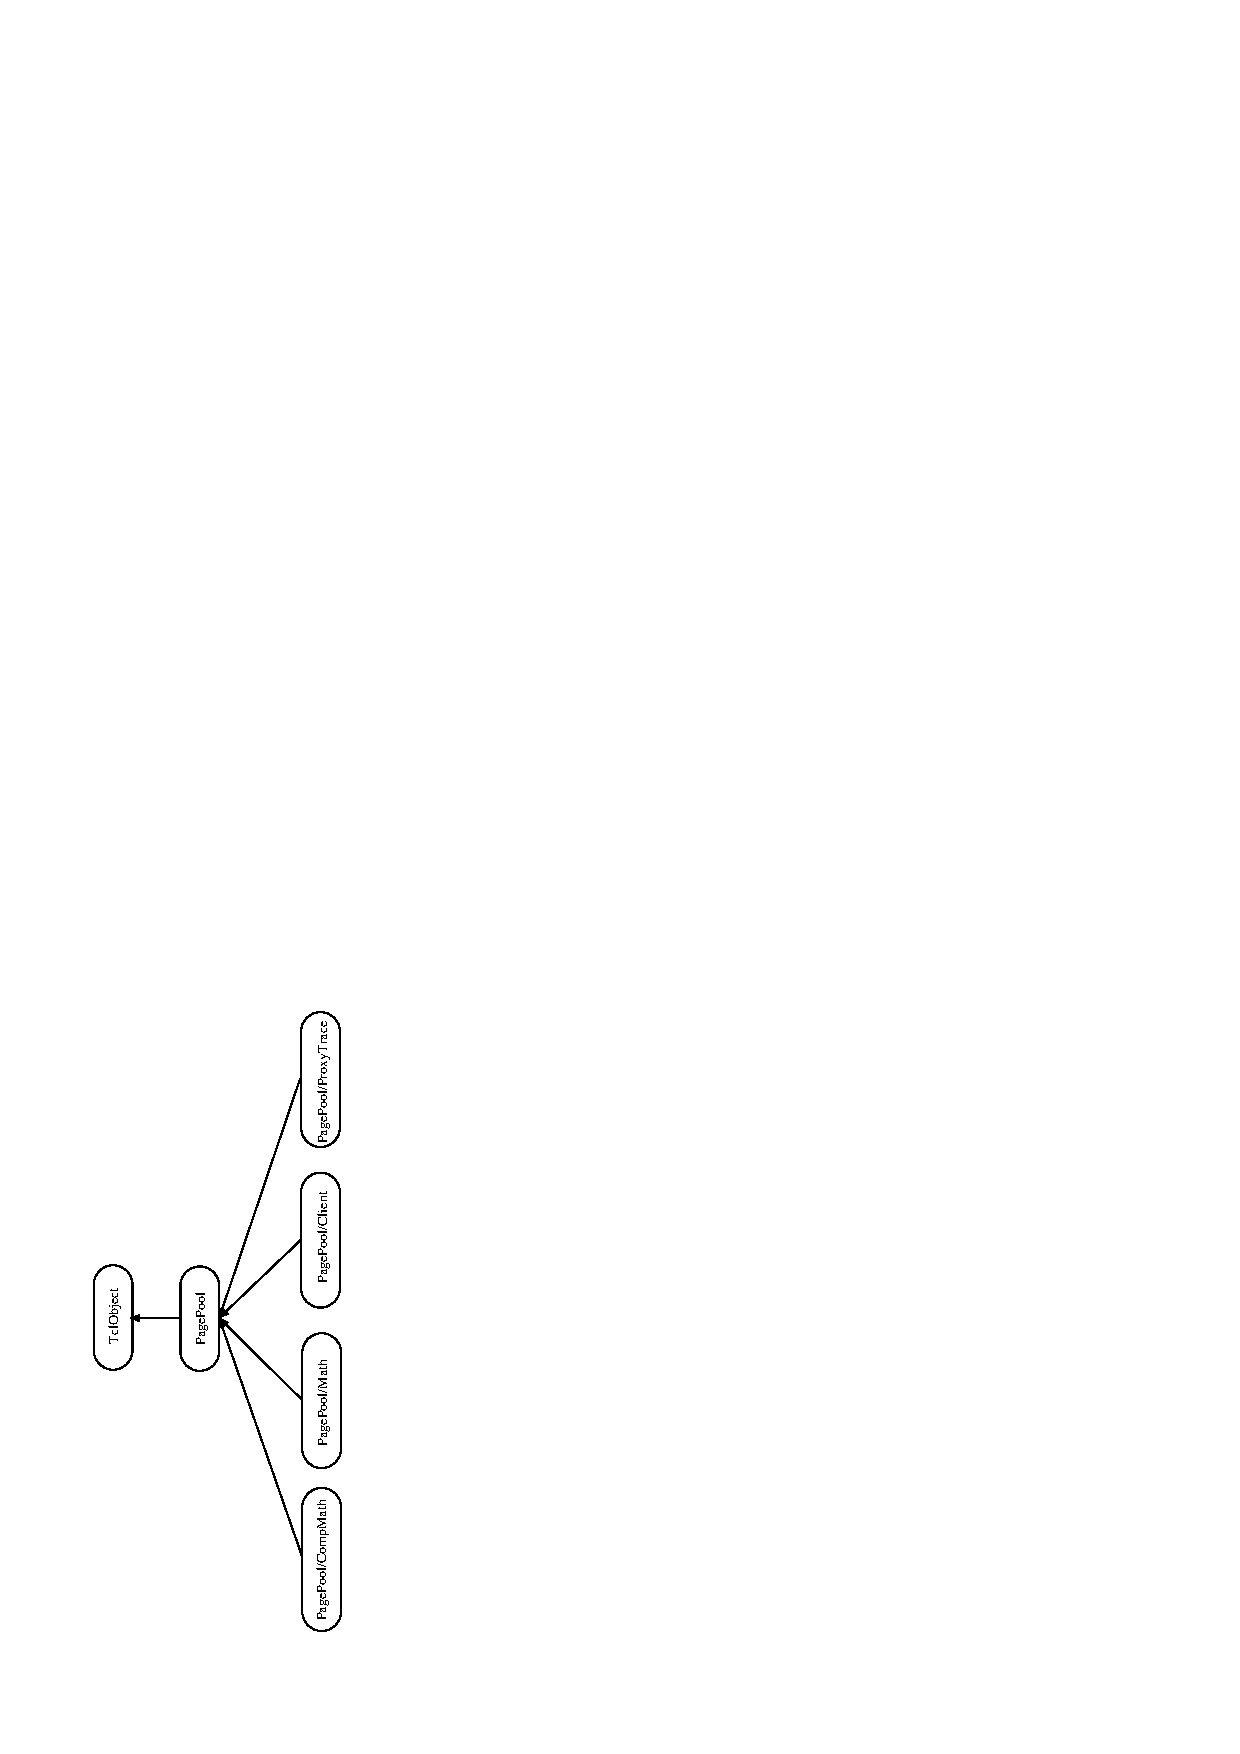
\includegraphics{pagepool-hier}
    \caption{Class hierarchy of page pools}
    \label{fig:pagepool-hier}
  \end{center}
\end{figure}

Among these, class PagePool/Client is mostly used by caches to store
pages and other cache-related information; other three classes are
used by servers and clients. In the following we describe these
classes one by one.

\subsection{PagePool/Math}

This is the simplest type of page pool. It has only one page, whose
size can be generated by a given random variable. Page modification
sequence and request sequence are 
generated using two given random variables. It has the following OTcl
methods:

\begin{alist}
gen-pageid & Returns the page ID which will be requested next. Because
 it has only one page, it always returns 0.\\

gen-size & Returns the size of the page. It can be generated by a
  given random variable. \\

gen-modtime \tup{pageID} \tup{mt} & Returns the next modification time of the
  page. \tup{mt} gives the last modification time. It uses the
  lifetime random variable. \\

ranvar-age \tup{rv} & Set the file lifetime random variable as
  \tup{rv}. \\

ranvar-size \tup{rv} & Set the file size random variable to be
  \tup{rv}. \\
\end{alist}

{\em NOTE}: There are two ways to generate a request sequence. With
all page pools except PagePool/ProxyTrace, request sequence is
generated with a random variable which describes the request
interval, and the \code{gen-pageid} method of other page pools gives
the page ID of the next request. PagePool/ProxyTrace loads the request
stream during initialization phase, so it does not need a random
variable for request interval; see its description below. 

An example of using PagePool/Math is at Section
\ref{sec:webcache-example}. That script is also available at 
\ns/tcl/ex/simple-webcache.tcl. 

\subsection{PagePool/CompMath}

It improves over PagePool/Math by introducing a compound page
model. By a compound page we mean a page which consists of a main text
page and a number of embedded objects, e.g., GIFs. We model a compound
page as a main page and several component objects. The main page is
always assigned with ID 0. All component pages
have the same size; both the main page size and component object size is
fixed, but adjustable through OTcl-bound variables \code{main_size_}
and \code{comp_size_}, respectively. The number of component objects
can be set using the OTcl-bound variable \code{num_pages_}.

PagePool/CompMath has the following major OTcl methods:

\begin{alist}
gen-size \tup{pageID} & If \tup{pageID} is 0, return
  \code{main\_size\_}, otherwise return \code{comp\_size\_}.\\

ranvar-main-age \tup{rv} & Set random variable for main page
  lifetime. Another one, \code{ranvar-obj-age}, set that for component
  objects. \\

gen-pageid & Always returns 0, which is the main page ID. \\ 

gen-modtime \tup{pageID} \tup{mt} & Returns the next modification time
  of the given page \tup{pageID}. If the given ID is 0, it uses the
  main page lifetime random variable; otherwise it uses the component
  object lifetime random variable. \\
\end{alist}

An example of using PagePool/CompMath is available at 
\ns/tcl/ex/simple-webcache-comp.tcl.

\subsection{PagePool/ProxyTrace}

The above two page pool synthesize request stream to a single web page
by two random variables: one for request interval, another for
requested page ID. Sometimes users may want more complicated request
stream, which consists of multiple pages and exhibits spatial locality
and temporal locality. There exists one proposal (SURGE
\cite{Barf98:WebWorkload}) 
which generates such request streams, we choose to provide an
alternative solution: use real web proxy cache trace (or server
trace). 

The class PagePool/ProxyTrace uses real traces to drive
simulation. Because there exist many web traces with different
formats, they should be converted into a intermediate format before
fed into this page pool. The converter is available at 
http://mash.cs.berkeley.edu/dist/vint/webcache-trace-conv.tar.gz.
It accepts four trace formats: DEC proxy trace (1996), UCB
Home-IP trace, NLANR proxy trace, and EPA web server trace. It
converts a given trace into two files: pglog and reqlog. Each line in
pglog has the following format:
\begin{center}
\begin{verbatim}
[<serverID> <URL_ID> <PageSize> <AccessCount>]
\end{verbatim}
\end{center}

Each line, except the last line, in reqlog has the following format:
\begin{center}
\begin{verbatim}
[<time> <clientID> <serverID> <URL_ID>]
\end{verbatim}
\end{center}

The last line in reqlog records the duration of the entire trace and
the total number of unique URLs:
\begin{center}
\begin{verbatim}
i <Duration> <Number_of_URL>
\end{verbatim}
\end{center}

PagePool/ProxyTrace takes these two file as input, and use them to
drive simulation. Because most existing web proxy traces do not
contain complete page modification information, we choose to use a
bimodal page modification model \cite{Cao97:CacheConsistency}. We
allow user to select $x\%$ of the pages to have one random page
modification interval generator, and the rest of the pages to have
another generator. In this way, it's possible to let $x\%$ pages to be
dynamic, i.e., modified frequently, and the rest static. Hot pages are
evenly distributed among all pages. For example, assume 10\% pages are
dynamic, then if we sort pages into a list according to their popularity,
then pages 0, 10, 20, $\ldots$ are dynamic, rest are static. Because
of this selection mechanism, we only allow bimodal ratio to change in
the unit of 10\%. 

In order to distribute requests to different requestors in the
simulator, PagePool/ProxyTrace maps the client ID in the traces to
requestors in the simulator using a modulo operation. 

PagePool/ProxyTrace has the following major OTcl methods:

\begin{alist}
get-poolsize & Returns the total number of pages. \\

get-duration & Returns the duration of the trace. \\

bimodal-ratio & Returns the bimodal ratio. \\

set-client-num \tup{num} & Set the number of requestors in the
simulation. \\

gen-request \tup{ClientID} & Generate the next request for the given
requestor. \\

gen-size \tup{PageID} & Returns the size of the given page. \\

bimodal-ratio \tup{ratio} & Set the dynamic pages to be \tup{ratio}*10
percent. Note that this ratio changes in unit of 10\%. \\

ranvar-dp \tup{ranvar} & Set page modification interval generator for 
dynamic pages. Similarly, ranvar-sp \tup{ranvar} sets the generator
for static pages. \\

set-reqfile \tup{file} & Set request stream file, as discussed
above. \\

set-pgfile \tup{file} & Set page information file, as discussed
above. \\

gen-modtime \tup{PageID} \tup{LastModTime} & Generate next
modification time for the given page. \\
\end{alist}

An example of using PagePool/ProxyTrace is available at 
\ns/tcl/ex/simple-webcache-trace.tcl. 


\subsection{PagePool/Client}

The class PagePool/Client helps caches to keep track of pages resident
in cache, and to store various cache-related information about
pages. It is mostly implemented in C++, because it is mainly used
internally and little functionality is needed by users. It has the
following major C++ methods:

\begin{itemize}
\item \code{get_page(const char* name)} - Returns a pointer to the
  page with the given name. 
\item \code{add_page(const char *name, int size, double mt,
    double et, double age)} - Add a page with given size, last modification
    time (mt), cache entry time (et), and page lifetime (age). 
\item \code{remove_page(const char* name)} - Remove a page from cache.
\end{itemize}

This page pool should support various cache replacement algorithms,
however, it has not been implemented yet. 


\section{Web client}
\label{sec:webcache-client}

Class Http/Client models behavior of a simple web browser. It
generates a sequence of page requests, where request interval and page 
IDs are randomized. It's a pure OTcl class inherited from Http. 
Next we'll walk through its functionalities and usage.

\paragraph{Creating a client}

First of all, we create a client and connect it to a cache and a web server.
Currently a client is only allowed to connect to a single cache, but it's 
allowed to connect to multiple servers. Note that this has to be called 
\emph{AFTER} the simulation starts (i.e., after \code{$ns run} %$
is called).
This remains true for all of the following methods and code examples of 
Http and its derived classes, unless explicitly said.

\begin{program}
        # Assuming $server is a configured Http/Server. 
        set client [new Http/Client $ns $node] \; client resides on this node;
        $client connect $server \; connecting client to server;
\end{program} %$

\paragraph{Configuring request generation}

For every request, Http/Client uses PagePool to generate a random page
ID, and use a random variable to generate intervals between two 
consecutive requests:
\footnote{Some PagePool,
e.g., PagePool/Math, has only one page and therefore it always returns the
same page. Some other PagePool, e.g. PagePool/Trace, has multiple pages 
and needs a random variable to pick out a random page.} 

\begin{program}
        $client set-page-generator $pgp \; attach a configured PagePool;
        $client set-interval-generator $ranvar \; attach a random variable;
\end{program}

Here we assume that PagePools of Http/Client share the same set of pages
as PagePools of the server. Usually we simplify our simulation by letting
all clients and servers share the same PagePool, i.e., they have the same
set of pages. When there are multiple servers, or servers' PagePools 
are separated from those of clients', care must be taken to make sure that 
every client sees the same set of pages as the servers to which they are
attached.

\paragraph{Starting}

After the above setup, starting requests is very simple:

\begin{program}
        $client start-session $cache $server \; assuming $cache is a configured Http/Cache;
\end{program}

\paragraph{OTcl interfaces}
Following is a list of its OTcl methods (in addition to those
inherited from Http). This is not a complete list. More details can be
found in \ns/tcl/webcache/http-agent.tcl.

\begin{alist}
send-request \tup{server} \tup{type} \tup{pageid} \tup{args} & 
send a request of page \$pageid and type \$type to \$server. The only 
request type allowed for a client is GET. \$args has a format identical
to that of \$attributes described in \code{Http::enter-page}. \\

start-session \tup{cache} \tup{server} & start sending requests of a 
random page to \$server via \$cache. \\

start \tup{cache} \tup{server} & before sending requests, populate
\$cache with all pages in the client's PagePool. This method is useful 
when assuming infinite-sized caches and we want to observe behaviors 
of cache consistency algorithms in steady state. \\

set-page-generator \tup{pagepool} & attach a PagePool to generate 
random page IDs.\\

set-interval-generator \tup{ranvar} & attach a random variable to generate
random request intervals.\\
\end{alist}


\section{Web server}
\label{seccom:webcache-server}

Class Http/Server models behavior of a HTTP server. Its
configuration is very simple. All that a user needs to do is to create 
a server, attach a PagePool and wait:

\begin{program}
        set server [new Http/Server $ns $node] \; attach \$server to \$node;
        $server set-page-generator $pgp \; attach a page pool;
\end{program}

An Http/Server object waits for incoming requests after simulation starts.
Usually clients and caches initiates connection to an Http/Server. But 
it still has its own \code{connect} method, which allows an Http/Server 
object to actively connect to a certain cache (or client). Sometimes this
is useful, as explained in Test/TLC1::set-groups\{\} in 
\ns/tcl/test/test-suite-webcache.tcl.

An Http/Server object accepts two types of requests: GET and IMS.  GET
request models normal client requests. For every GET request, it
returns the attributes of the requested page.  IMS request models
If-Modified-Since used by TTL algorithms for cache consistency. For
every IMS (If-Modified-Since) request, it compares the page
modification time given in the request and that of the page in its
PagePool. If the time indicated in the request is older, it sends back
a response with very small size, otherwise it returns all of the page 
attributes with response size equal the real page size.


\section{Web cache}
\label{sec:webcache-cache}

Currently 6 types of web caches are implemented, including 
the base class Http/Cache. Its five derived subclasses 
implement 5 types of cache consistency algorithms: Plain old TTL, 
adaptive TTL, Omniscient TTL, Hierarchical multicast invalidation, 
and hierarchical multicast invalidation plus direct request.

In the following we'll only describe the base class Http/Cache, because 
all the subclasses involves discussion of cache consistency algorithms 
and it does not seem to be appropriate here.

\subsection{Http/Cache}
\label{sec:webcache-cache-base}

Class Http/Cache models behavior of a simple HTTP cache with infinite 
size. It doesn't contain removal algorithm, nor consistency algorithm. 
It is not intended to be used by itself. Rather, it is meant to be a 
base class for experimenting with various cache consistency algorithms and
other cache algorithms. 

\paragraph{Creation and startup}

Creating an Http/Cache requires the same set of parameters as
Http/Client and Http/Server. After creation, a cache needs to connect 
to a certain server. Note that this creation can also be done dynamically,
when a request comes in and the cache finds that it's not connected to 
the server. However, we do not model this behavior in current code.
Following code is an example:

\begin{program}
        set cache [new HttpCache $ns $node] \; attach cache to \$node;
        $cache connect $server \; connect to \$server;
\end{program}

Like Http/Server, an Http/Cache object waits for requests (and packets
from server) after it's initialized as above. When hierarchical
caching is used, the following can be used to create the hierarchy:

\begin{program}
        $cache set-parent $parent \; set parent cache;
\end{program}

Currently all TTL and multicast invalidation caches support hierarchical
caching. However, only the two multicast invalidation caches allows 
multiple cache hierarchies to inter-operate.

\paragraph{OTcl methods}

Although Http/Cache is a SplitObject, all of its methods are in OTcl. 
Most of them are used to process an incoming request. Their relations can
be illustrated with the flowchart below, followed by explainations:

\begin{figure}[h]
  \begin{center}
    \includegraphics{cache-flowchart}
    \caption{Handling of incoming request in Http/Cache}
    \label{fig:webcache-handle-request}
  \end{center}
\end{figure}

\begin{alist}
get-request \tup{client} \tup{type} \tup{pageid} & 
The entry point of processing any request. It checks if the requested 
page \$pageid exists in the cache's page pool, then call either 
\code{cache-hit} or \code{cache-miss}. \\

cache-miss \tup{client} \tup{type} \tup{pageid} & 
This cache doesn't have the page. Send a request to server (or parent 
cache) to refetch the page if it hasn't already done so. Register 
\$client in a list so that when the cache gets the page, it'll forward
the page to all clients who have requested the page. \\

cache-hit \tup{client} \tup{type} \tup{pageid} &
Checks the validatity of the cached page. If it's valid, send \$client
the cached page, otherwise refetch the page. \\ 

is-consistent \tup{client} \tup{type} \tup{pageid} & 
Returns 1 if \$pageid is valid. This is intended to be overridden by 
subclasses. \\

refetch \tup{client} \tup{type} \tup{pageid} & 
Refetch an invalid page from server. This is intended to be overridden 
by subclasses. \\
\end{alist}


\section{Putting together: a simple example}
\label{sec:webcache-example}

We have seen all the pieces, now we present a script which provides a
complete view of all pieces together. First, we build topology and 
other usual initializations:

\begin{program}
        set ns [new Simulator]

        # Create topology/routing
        set node(c) [$ns node] 
        set node(e) [$ns node]
        set node(s) [$ns node]
        $ns duplex-link $node(s) $node(e) 1.5Mb 50ms DropTail
        $ns duplex-link $node(e) $node(c) 10Mb 2ms DropTail 
        $ns rtproto Session
\end{program}

Next we create the Http objects:

\begin{program}
        # HTTP logs
        set log [open "http.log" w]

        # Create page pool as a central page generator. Use PagePool/Math
        set pgp [new PagePool/Math]
        set tmp [new RandomVariable/Constant] \;# Page size generator;
        $tmp set val_ 1024  \;# average page size;
        $pgp ranvar-size $tmp
        set tmp [new RandomVariable/Exponential] \;# Page age generator;
        $tmp set avg_ 5 \;# average page age;
        $pgp ranvar-age $tmp

        set server [new Http/Server $ns $node(s)] \;# Create a server and link it to the central page pool;
        $server set-page-generator $pgp
        $server log $log

        set cache [new Http/Cache $ns $node(e)] \;# Create a cache;
        $cache log $log

        set client [new Http/Client $ns $node(c)] \;# Create a client;
        set tmp [new RandomVariable/Exponential] \;# Poisson process as request sequence;
        $tmp set avg_ 5 \;# average request interval;
        $client set-interval-generator $tmp
        $client set-page-generator $pgp
        $client log $log

        set startTime 1 \;# simulation start time;
        set finishTime 50 \;# simulation end time;
        $ns at $startTime "start-connection"
        $ns at $finishTime "finish"
\end{program} %$

Then we define a procedure which will be called after simulation
starts.  The procedure will setup connections among all Http objects.
\begin{program}
        proc start-connection {} {
                global ns server cache client
                $client connect $cache
                $cache connect $server
                $client start-session $cache $server
        }
\end{program} %$

At the end, the usual closing:
\begin{program}
        proc finish {} {
                global ns log
                $ns flush-trace
                flush $log
                close $log
                exit 0
        }
        $ns run
\end{program}

This script is also available at \ns/tcl/ex/simple-webcache.tcl. 
Examining its output \code{http.log}, one will find that the result of 
the absense cache consistency algorithm results in a lot of stale hits. 
This can be easily remedied by replacing ``new Http/Cache'' line with:
\code{set cache [new Http/Cache/TTL $ns $node(e)]}. For more complicated
cache consistency algorithm examples, see 
\ns/tcl/test/test-suite-webcache.tcl.

\section{Http trace format}
\label{sec:webcache-trace}

The trace file of Http agents are constructed in a similar way as the
SRM trace files. It consists of multiple entries, each of which
occupies one line.  The format of each entry is:

\begin{tabular}[h]{c|c|c}
  Time & ObjectID & Object Values
\end{tabular}

There are three types of objects: client ({\bf C}), cache ({\bf E})
and server ({\bf S}). Following is a complete enumeration of all possible 
events and value types associated with these three types of objects.

\begin{center}
  \begin{tabular}[h]{c|c|l}
    \emph{Object Type} & \emph{Event Type} & \emph{Values} \\ \hline
    E & HIT & \tup{Prefix} \\
    E & MISS & \tup{Prefix} z \tup{RequestSize} \\
    E & IMS & \tup{Prefix} z \tup{Size} t \tup{CacheEntryTime} \\
    E & REF & p \tup{PageID} s \tup{ServerID} z \tup{Size} \\
    E & UPD & p \tup{PageID} m \tup{LastModifiedTime} z \tup{PageSize} \\
    &     & s \tup{ServerID} \\ 
    E & GUPD & z \tup{PageSize} \\
    E & SINV & p \tup{PageID} m \tup{LastModTime} z \tup{PageSize} \\
    E & GINV & p \tup{PageID} m \tup{LastModTime} \\
    E & SPF & p \tup{PageID} c \tup{DestCache} \\
    E & RPF & p \tup{PageID} c \tup{SrcCache} \\
    E & ENT & p \tup{PageID} m \tup{LastModifiedTime} z \tup{PageSize} \\
    &     & s \tup{ServerID} \\ \hline
    C & GET & p \tup{PageID} s \tup{PageServerID} z \tup{RequestSize}\\
    C & STA & p \tup{PageID} s \tup{OrigServerID} l \tup{StaleTime}\\
    C & RCV & p \tup{PageID} s \tup{PageServerID} l \tup{ResponseTime} z \tup{PageSize}\\ \hline
    S & INV & p \tup{PageID} m \tup{LastModifiedTime} z \tup{Size} \\
    S & UPD & p \tup{PageID} m \tup{LastModifiedTime} z \tup{Size} \\
    S & SND & p \tup{PageID} m \tup{LastModifiedTime} z \tup{PageSize} \\
      &     & t \tup{Requesttype} \\
    S & MOD & p \tup{PageID} n \tup{NextModifyTime} \\
  \end{tabular}
\end{center}

\tup{Prefix} is the information common to all trace entries. It includes:

\begin{center}
  \begin{tabular}[h]{c|c|c}
    p \tup{PageID} & c \tup{RequestClientID} & s \tup{PageServerID}
  \end{tabular}
\end{center}

\emph{Short Explaination of event operations}: 

\begin{center}
  \begin{tabular}[h]{c|c|l}
    \emph{Object Type} & \emph{Event Type} & \emph{Explaination} \\ \hline
    E & HIT & Cache hit. PageSererID is the id of the ``owner'' of the page. \\
    E & MISS & Cache miss. In this case the cache will send a request to the
    server to fetch the page. \\
    E & IMS & If-Modified-Since. Used by TTL procotols to validate an expired 
    page. \\
    E & REF & Page refetch. Used by invalidation protocols to refetch an 
    invalidated page. \\
    E & UPD & Page update. Used by invalidation protocols to ``push'' updates\\
      & & from parent cache to children caches. \\
    E & SINV & Send invalidation. \\
    E & GINV & Get invalidation. \\
    E & SPF & Send a pro forma \\
    E & RPF & Receive a pro forma \\
    E & ENT & Enter a page into local page cache. \\ 
    \hline
    C & GET & Client sends a request for a page. \\
    C & STA & Client gets a stale hit. OrigModTime is the modification time \\
    & & in the web server, CurrModTime is the local page's modification time.\\
    C & RCV & Client receives a page. \\
    \hline
    S & SND & Server send a response. \\
    S & UPD & Server pushes a page update to its ``primary cache''. Used by
    invalidation protocol only. \\
    S & INV & Server sends an invalidation message. Used by invalidation 
    protocol only. \\
    S & MOD & Server modified a page. The page will be modified next
    at \tup{NextModifyTime}. \\
  \end{tabular}
\end{center}


\endinput

% Local Variables:
% TeX-master: "everything"
% LocalWords:
% End:
% LocalWords:  HTTP tb app dataflow ADU OTcl AppData AppDataType struct hdr buf
% LocalWords:  const AppConnector inline int TclCL HttpApp webcache http nbytes
% LocalWords:  userdata HttpInvalAgent inteded inval recv realsize inv FullTcp
% LocalWords:  SimpleTcp bi str dsize Tcl tcl tcp iss ns TcpApps Mb ms DropTail
% LocalWords:  tmp val RandomVariable pgp ranvar avg startTime finishTime proc


\part{Scale}
\chapter{Session-level Packet Distribution}
\label{chap:session}

This section describes the internals of the Session-level Packet Distribution
implementation in \ns.
The section is in two parts:
the first part is an overview of 
a basic Session configuration,
and a ``complete'' description of the configuration parameters 
of a Session.
The second part describes the architecture, internals, and the code path
of the Session-level Packet distribution.

Session-level Packet Distribution enables simulations with large-scale 
topologies.  A 2048 node and 8 connectivity degree topology takes roughly 
40 MB in memory, 2049-4096 node topology takes about 167 MB, and 4097-
8194 node topology takes about 671 MB.  However, the queuing delays that
may occur in routers are ignored.  Therefore, if simulations are involved 
with high source rate or multiple sources merging at some point resulting
a high aggregated rate, please avoid using Session-level Packet Distribution.

\section{Configuration}

\subsection{Basic Configuration}
\label{sec:basic-config}

Each Session (i.e., a multicast tree) must be configured strictly in
this order:
creating(obtaining) the session source,
assigning the destination address,
creating the session helper, 
attaching to session source, and
the session members joining the group.


\begin{program}
        set ns [new SessionSim]          \; preamble initialization;
        set node [$ns node]              \; source and receiver to reside on this node;
        set group [$ns allocaddr]        \; multicast group for this session;

        set src [new Agent/CBR]
        $src set dst_ $group            \; configure the source;
        $ns attach-agent $node $src

        $ns create-session $node $src   \; creating the session helper and attaching to the source;

        set rcvr [new Agent/NULL]        \; configure the receiver;
        $ns attach-agent $node $rcvr
        $ns at 0.0 "$node join-group $rcvr $group" \; joining the session;

        $ns at 0.1 "$src start"          \; start the source;

\end{program}

\subsection{Inserting a Loss Module}
\label{sec:loss-config}

When simulating mechanism robustness(e.g., SRM error recovery mechanism), 
modules like lossy links are desired to create error senarios.  This 
subsection is describe how to create a lossy link, meaning inserting 
a loss module for a 'virtual link' (a link directly connecting source
and receiver with accumulative bandwidth and delay).

Please note that packets dropped at a particular link in a
multicast tree will not be received by
the receivers in the particular downstream subtree. We have worked 
on this dependency problem and now the loss modules for the downstream 
receivers will be installed automatically when a lossy link is created.


\paragraph{Creating a Loss Module}
Before we can insert a loss module in between a source-receiver pair,
we have to create the loss module.  Basically,
a loss module compares two values to decide whether to drop a packet.
The first value is obtained every time when the loss module receives 
a packet from a random variable.  The second value
is fixed and configured when the loss module is created.

The following code gives an example to create a uniform 
0.1 loss rate.

\begin{program}
        # creating the uniform distribution random variable
        set loss_random_variable [new RandomVariable/Uniform] 
        # setting the range of random variable
        $loss_random_variable set min_ 0
        $loss_random_variable set max_ 100

        # creating an error module;
        set loss_module [new ErrorModel]
        # set target for dropped packets;
        $loss_module drop-target [new Agent/Null]
        # setting error rate to 0.1, 10/(100-0);
        $loss_module set rate_ 10
        # attaching the random variable to the loss module;
        $loss_module ranvar $loss_random_variable 

\end{program}

Several random variable distributions are available.
%%% Need xref to ranvar pages
Please refer to tcl/ex/ranvar.tcl.

\paragraph{Inserting a Loss Module}

If it is intended to insert a loss module for a receiver, keep a handle to the 
loss module when created.  Loss modules can only be inserted after the
corresponding receivers finish joining the group.

\begin{program}
        # keep a handle to the loss module;
        set sessionhelper [$ns create-session $node $src] 
        # insert the loss module;
        $ns at 0.1 "$sessionhelper insert-depended-loss $loss_module $rcvr" 
\end{program}

\section{Architecture}
\label{sec:session-arch}
The purpose of Session-level packet distribution is to
speed up simulations and reduce memory consumption while 
maintaining reasonable accuracy(if no queuing involved).  The first
bottleneck observed is the memory consumption by heavy-weight
links and nodes.  Therefore, in SessionSim (Simulator for Session-level
packet distribution), we keep only minimal amount of 
states for links and nodes, and connect the higher level source and 
receiver applications with appropriate delay and loss modules.  When
a connection is a multicast group, we attach a replicator 
to the source application, so the replicator replicates packets
to all loss or delay modules attached to the receiver applications.

In short, almost the entire network layer(routing and queuing)
is abstract out.  Packets in SessionSim do not get routed.  
They only follow the established Session.

\section{Internals}
In this section, we explain the internals of Session-level Packet 
Distribution.  The implementation is split into two parts:
\begin{list}{}{}
\item  Linkage of objects to make a Session in OTcl 
\item  Packet forwarding activities are executed by C++ methods.  
\end{list}

\subsection{Object Linkage}
\label{sec:session-objlink}

\begin{list}{}{}
\item  Simplified links and nodes.
\item  Replicator
\item  Delay and loss modules
\end{list}

\paragraph{Nodes and Links}
A link only contains the values of
its bandwidth and delay, and a node contains only its id and port number
for next agent.

\begin{program}
SessionSim instproc simplex-link \{ n1 n2 bw delay type \} \{
    $self instvar bw_ delay_
    set sid [$n1 id]
    set did [$n2 id]

    set bw_($sid:$did) [expr [string trimright $bw Mb] * 1000000]
    set delay_($sid:$did) [expr [string trimright $delay ms] * 0.001]
\}

SessionNode instproc init \{\} \{
    $self instvar id_ np_
    set id_ [Node getid]
    set np_ 0
\}
\end{program}

\paragraph{Replicator}
One replicator is required per source.  While the source is configured,
a replicator (session helper) need to be attached to the source.  By
calling \proc[]{create-session}, a replicator is:
created,
attached to the source application, and 
kept in a SessionSim instance variable \code{session_} array with 
its source and destination addresses as the index.

Note that the destination of source agent must be set before
calling \proc[]{create-session}.

\begin{program}
SessionSim instproc create-session \{ node agent \} \{
    $self instvar session_

    set nid [$node id]                           \; get source address;
    set dst [$agent set dst_]                    \; get destination address;
    set session_($nid:$dst) [new Classifier/Replicator/Demuxer]  \; creating the replicator;
    $agent target $session_($nid:$dst)           \; attach the replicator to the source;
    return $session_($nid:$dst) \; keep the replicator in the SessionSim instance variable session_ array;
\}
\end{program}

\paragraph{Delay and Loss Modules}

At least one delay module is required per receiver.
See Section~\ref{sec:loss-config} for inserting a loss module for a receiver.
When a receiver joins a group, 
the \proc[]{join-group} method goes through
all replicators (session helpers) maintained in \code{session_}.
If the destination index matches the group address
the receiver are joining, then the following actions are performed.

1. A new slot of the replicator (session helper) is created and assigned to the receiver.

2. An accumulated bandwidth and delay between the source and receiver are obtained by SessionSim instance procedure \proc[]{get-bw} and \proc[]{get-delay}.

3. A constant random variable is created and assigned with the
accumulative delay.

4. A delay module is created and assigned with the constant random 
variable and the accumulative bandwidth.

5. The delay module in inserted into the replicator slot in
front of the receiver.

\begin{program}
SessionSim instproc join-group \{ agent group \} \{
    $self instvar session_

    foreach index [array names session_] \{
        set pair [split $index :]
        if \{[lindex $pair 1] == $group\} \{
            # Note: must insert the chain of loss, delay, 
            # and destination agent in this order:

            #1. insert destination agent into session replicator
            $session_($index) insert $agent

            #2. find accumulative bandwidth and delay
            set src [lindex $pair 0]
            set dst [[$agent set node_] id]
            set accu_bw [$self get-bw $dst $src]
            set delay [$self get-delay $dst $src]

            #3. set up a constant delay random variable
            set random_variable [new RandomVariable/Constant]
            $random_variable set avg_ $delay

            #4. set up the delay module
            set delay_module [new DelayModel]
            $delay_module bandwidth $accu_bw
            $delay_module ranvar $random_variable

            #5. insert the delay module in front of the dest agent
            $session_($index) insert-module $delay_module $agent
        \}
    \}
\}
\end{program}


\subsection{Packet Forwarding}
\label{sec:session-pktforward}
Packet forwarding activities are executed in C++.  A source application 
generates a packet and forwards to its target which must be a replicator 
(session helper).  The replicator copies the packet and forwards 
to targets in the active slots which are either delay modules or loss modules. If loss modules, a decision is made whether to drop the packet.
If yes, the packet is forwarded to the loss modules drop target.  If not,
the loss module forwards it to its target which must be a delay module.
The delay module will forward the packet with a delay to its target which
must be a receiver application.

%% PH: not sure this will come out right
%% PH: make .eps picture but not sure how to import that

\begin{program}
                    / Loss module - Delay module - Receiver 1
Source - Replicator --------------- Delay module - Receiver 2
    (Session Helper)\bs Loss module - Delay module - Receiver 3

\end{program}

\endinput

### Local Variables:
### mode: latex
### comment-column: 60
### backup-by-copying-when-linked: t
### file-precious-flag: nil
### End:


\part{Emulation}
\chapter{Emulation}
\label{sec:emulation}

This chapter describes the {\em emulation} facility
of \ns.
Emulation refers to the ability to introduce the
simulator into a live network.
Special objects within the simulator are capable
of introducing live traffic into the simulator and
injecting traffic from the simulator into the
live network.

\section{Introduction}

The emulation facility can be subdivided into
two modes:
\begin{enumerate}
\item {\sf opaque mode} -- live data treated as opaque data packets
\item {\sf protocol mode} -- live data may interpreted/generated by simulator
\end{enumerate}
In opaque mode, the simulator
treats network data as uninterpreted packets.
In particular, real-world protocol fields
are not directly manipulated by the simulator.
In opaque mode, live data packets may be dropped, delayed, re-ordered, or
duplicated, but because no protocol processing is performed,
protocol-specific traffic manipulation scenarios (e.g. ``drop the TCP segment
containing a retransmission of sequence number 23045'') may not be performed.
In protocol mode, the simulator is able to interpret and/or generate
live network traffic containing arbitrary field assignments.
{\bf To date (Mar 1998), only Opaque Mode is currently implemented}.

The interface between the simulator and live network is provided by
a collection of objects including {\em tap agents} and {\em network objects}.
Tap agents embed live network data into simulated packets and
vice-versa.
Network objects are installed in tap agents and provide an entrypoint
for the sending and receipt of live data.
Both objects are described in the following sections.

\section{Tap Agents}

The class {\tt TapAgent} is a simple class derived from the base
{\tt Agent} class.
As such, it is able to generate simulator packets containing
arbitrarily-assigned values within the \ns common header.
The tap agent handles the setting of the common header packet
size field and the type field.  
It uses the packet type {\tt PT\_LIVE} for packets injected
into the simulator.
Each tap agent can have at most one associated network object, although
more than one tap agent may be instantiated on a single simulator node.

\paragraph{Configuration}
Tap agents are able to send and receive packets to/from an
associated {\tt Network} object.
Assuming a network object {\tt \$netobj} refers to a network
object, a tap agent is configured using the {\tt network} method:
\begin{verbatim}
        set a0 [new Agent/Tap]
	$a0 network $netobj
	$a0 set fid_ 26
	$a0 set prio_ 2
	$ns connect $a0 $a1
\end{verbatim}
Note that the configuration of the flow ID and priority are
handled through the {\tt Agent} base class.
The purpose of setting the flow id field in the common header
is to label packets belonging to particular flows of live data.
Such packets can be differentially treated with respect
to drops, reorderings, etc.
The {\tt connect} method instructs agent {\tt \$a0} to send
its live traffic to the {\tt \$a1} agent via the current
route through the simulated topology.

\section{Network Objects}

\endinput


\part{Visualization with Nam - The Network Animator}

\chapter{Nam}
\label{chap:nam}


\section{Introduction}

Nam is a Tcl/TK based animation tool for viewing network simulation traces and real world packet tracedata. The design theory behind nam was to create an animator that is able to read large animation data sets and be extensible enough so that it could be used indifferent network visualization situations.  Under this constraint nam was designed to read simple animation event commands from a large trace file.  In order to handle large animtion data sets a minimum amount of information is kept in memory.  Event commands are kept in the file and reread from the file whenever necessary.

The first step to use nam is to produce the trace file. The trace file contains topology information, e.g., nodes, links, as well as packet traces. The detailed format is described in the section \ref{sec:namtraceformat}. Usually, the trace file is generated by ns. During an ns simulation, user can produce topology configurations, layout information, and packet traces using tracing events in ns.  However any application can generate a nam trace file.

When the trace file is generated, it is ready to be animated by nam. Upon startup, nam will read the tracefile, create topology, pop up a window, do layout if necessary, and then pause at time 0. Through its user interface, nam provides control over many aspects of animation. These functionalities will be described in detail in the USER INTERFACE section.

There are bugs in nam however each successive has become much more stable than the previous one.  Please  mail ns-users@isi.edu if you encounter any bugs, or have suggestions for addiotional desired functionality.

\section{Nam Command Line Options}
\label{sec:namcommandlineoptions}
\begin{program}
nam [ -g <geometry> ] [ -t <graphInput> ] [ -i <interval> ] [ -j <startup time> ] 
    [ -k <intial socket port number> ] [ -N <application name> ] [ -c <cache size> ] 
    [ -f <configuration file> ] [ -r initial animation rate ]
    [ -a ] [ -p ] [ -S ]
    [ <tracefile(s)> ]
\end{program}

\textbf{Command Line Options}

\begin{tabular}{ll}
-g & Specify geometry of the window upon startup. \\

-t & Instruct nam to use tkgraph, and specify input file nam for tkgraph. \\

-i & [Information  for  this  option  may  not  be  accurate]  Specify rate (real)  milliseconds  as  the  screenupdate rate. The default rate is 50ms (i.e., 20 frames per second). Note that the X server may not be able to keep up with this rate, in which case the animation will run as fast as the X server allowsit to (at 100\% cpu utilization). \\
-N & Specify the application name of this nam instance. This application name may later be used in peer synchronization. \\
-c & The  maximum  size  of  the  cache  used  to  store  'active' objects when doing animating in reverse. \\
-f & Name of the initialization files to be loaded during startup. In this file, user can define functions which will be called in the trace file. An example for this is the 'link-up' and 'link-down' events of dynamic links in ns. (Refer to \$ns rtmodel for detail, and tcl/ex/simple-dyn.tcl in your ns direc-tory for example). Example initialization files can be found at ex/sample.nam.tcl and ex/dynamicnam.conf. \\
-a & Create a separate instance of nam. \\
-p & Print out nam trace file format. \\
-S & Enable synchronous X behavior so it is easier for graphics debugging. For UNIX system running X only. \\
<tracefile> & is the name of the file containing the trace data to be animated.  If <tracefile> cannot be read, nam will try to open <tracefile>.nam. \\
\end{tabular}


\section{User Interface}
\label{sec:userinterface}

Starting up nam will first create the nam console window.  You can have multiple animations running under the same nam instance.  At the top of all nam windows is a menu bar.  For the nam console there are 'File' and 'Help' menus.  Under the 'File' there is a 'New' command for creating a ns topology using the nam editor (under construction) , an 'Open' command which allows you to open existing tracefiles, a 'WinList' command that popup a window will the names of all currently opened tracefiles, and a 'Quit' command which exits nam. The 'Help' menu contains a very limited popup help screen and a command to show version and copyright information. 

Once a tracefile has been loaded into nam (either by using the 'Open' menu command or by specifying the tracefile on the command line) an animation window will appear.  It has a 'Save layout' command which will save the current network layout to a file and a 'Print' command which will print the current network layout.

The 'Views' menu has 4 buttons:
\begin{itemize}
\item New view button: Creates a new view of the same animation. User can scroll and zoom on the newview. All views will be animated synchronously.
\item  Show monitors checkbox: If checked, will show a pane at the lower half of window, where moni-tors will be displayed.
\item  Show autolayout checkbox: If checked, will show a pane at the lower half of window, which con-tains input boxes and a button for automatic layout adjustments. This box will not be enabled when using link orientain layouts.
\item Show annotation checkbox: If checked, will show a listbox at the lower half of window, which will be used to list annotations in the ascending order of time.
\end{itemize}

Below the  menu  bar, there  is  a control  bar containing  6  buttons,  a  label,  and  a  small  scrollbar(scale). They can be clicked in any order. We will explain them from left to right.

\begin{itemize}
\item Button 1 (<<) - Rewind. When clicked, animation time will go back at the rate of 25  times the current screen update rate.
\item  Button 2 (<) - Backward play. When clicked, animation will be played backward with time decreasing.
\item Button 3 (square) - Stop. When clicked, animation will pause.
\item Button 4 (>)  - Forward play. When clicked, animation will be played forward with time increasing.
\item Button 5 (>>) - Fast  Forward.  When  clicked,  animation  time  will  go  forward  at  the  rate  of  25  times  the  current screen update rate.
\item Button 6 (Chevron logo) - Close current animation window.
\end{itemize}

Time label - Show the current animation time (i.e., simulation time as in the trace file). 
Rate Slider - Controls the screen update rate (animation granularity). The current rate is displayed in the label above the slider.


Below the first control bar, there is Main Display, which contains a tool bar and a main view pane with two panning scroll bars. All new views created by menu command  'Views/New view' will have these three components. The  tool bar contains two zoom buttons. The  button with an up arrow zooms in, the button with a down arrrow zooms out. The two scroll bars are used to pan the main animation view. 

Clicking the left button on any of the objects in the main view pane will pop up a information window. For packet and agent objects, there is a 'monitor' button in the popup window. Clicking that  button  will  bring  out  the  monitor  pane (if  it  is  not already there),  and add a monitor to the object.  For link objects, there will be a 'Graph' button. Clicking on that button will bring up another popup window, where users can select between drawing a bandwidth  utilization graph or drawing a link loss graph of one simplex edge of the duplex link.

Below the user interface objects we have discussed  so  far, there  may  or  may  not  be  a Monitor  pane, depending  on whether the checkbox 'Views/Show monitors' is set. (The default is unset). All monitors will be shown in this pane. A monitor looks like a big button in the pane. Currently only packets and agents may have monitors.

 A packet monitor shows the size, id, and sent time. When the packet reaches its destination, the monitor will still be there, but will say that the packet is invisible. An agent monitor shows the name of the agent, and if there are any variable traces associated with this agent, they will be shown there as well.
 
Below the monitor pane (or in its place if the monitor pane isn't there), there is a Time Slider. It looks likea scaled ruler, with a tag 'TIME' which can be dragged along the ruler. It is used to set the current animation time.  As you drag the 'TIME' tag, current animation time will be displayed in the time label in the control bar above. The left edge of the slider represents the earliest event time in the trace file and the right edge represents the last event time. Clicking left button on the ruler (not on the tag) has the same effect as Rewind or Fast Forward, depending on the clicking position.

The Automatic Layout Pane may be visible or hidden. If visible, it is below the time slider. It has three inputboxes and one relayout button. The labeled input boxes let user adjust two automatic layout constants, and the number of iterations during next layout. When user press ENTER in any of the input boxes, or click the'relayout' button, that number of iterations will be performed. Refer to the AUTOMATIC LAYOUT section for details of usage.

 The bottom component of the nam window is a Annotation Listbox, where annotations are displayed. Anannotation is a (time, string) pair, which describes a event occuring at that time. Refer to ns(1) for functions to generate annotations. Double-clicking on an annotation in the listbox will bring nam to the time when that annotation is recorded. When the pointer is within the listbox,  clicking the right button will stop the animation and bring up a popup menu with 3 options: Add, Delete, Info. 'Add' will bring up a dialog box with a text input to add a new annotation entry which has the current animation time. The user can type an annotation string in the dialog box. `Delete' will delete the annotation entry pointed by the pointer. `Info' will bring out a pane which shows both the annotation time and the annotation string.

\section{Keyboard Commands}
\label{sec:keyboardcommands}
Most of the buttons have keyboard equivalents. Note they only function when the mouse cursor is inside the nam window.

\begin{itemize}
\item <return> - Typing a <return> will pause nam if it's not already paused. If nam is paused, <return> will step the animation one simulated clock tick. (If your keyboard autorepeats, holding down <return> is a goodway to slow-step through the animation.)
\item 'p' or 'P' - Pause but not step if paused.
\item 'c' or 'C' - Continue after a pause.
\item 'b' or 'B' - Decrease animation time for one screen update interval.
\item 'r' or 'R' - Rewind.
\item 'f' or 'F' - Fast Forward.
\item 'n' or 'N' - Jump to time of next event in the tracefile.
\item 'x' or 'X' - Undo the last rate change.
\item 'u' or 'U' - Undo the last time slider drag.
\item '>' or `.' Increase the granularity (speed up) by 5\%.
\item '<' or ',' Decrease the granularity (slow down) by 5\%.
\item <space bar> -  Toggle the pause state of nam. 
\item 'q', 'Q' or <control-c> - Quit.
\end{itemize}

\section{Generating External Animations from Nam}
\label{sec:exteranlanimations}

Nam animations can be saved and converted to animated gifs or MPEG movies.

To save the frames of your movie, first start nam with your trace and set it up where you want it to start and adjust other parameters (step rate, size, etc.) Select 'Record Animation' from the File menu to start saving frames.  Each animation step will be saved in a X-window dump file called ``nam\%d.xwd'' where \%d is the frame number. These files can then be assembled into animated GIFs or MPEGs with the appropriate post-processing tools.

The following shell script (sh, not csh) converts these files into an animated gif:
\begin{program}
    for i in *.xwd; do
    	xwdtoppm <$i |
    	ppmtogif -interlace -transparent'#e5e5e5' >`basename $i .xwd`.gif;
    done
    gifmerge -l0 -2 -229,229,229 *.gif >movie.gif
\end{program}

Please note that the programs xwdtoppm, ppmtogif, and gifmerge are \emph{not} part of ns.
You can get the first two from
\url{http://download.sourceforge.net/netpbm/}
and gifmerge from
\url{http://www.the-labs.com/GIFMerge/}.


\section{Network Layout}
\label{sec:networklayout}

In nam, a topology is specified by alternating node objects with edge objects. But to display the topology in a comprehensible way, a layout mechanism is needed. Currently nam provides three layout methods. First, user may specify layout by the link's orientation. A link orientation is the angle between the edge and a horizontal line, in the interval [0, 2$\pi$]. During layout, nam will honor the given link orientation. Generally, it will first choose a reference node, then place other nodes using link orientations and link length.  The link length is determined by link delay and connecting node sizes. This works well for small and manually generated topologies.

Second, when dealing with randomly generated topologies, we may want to do layout automatically. An automatic graph layout algorithm has been adapted and implemented. The basic idea of the algorithm is to model the graph as balls (nodes) connected by springs (links). Balls will repulse each other, while springs pull them together. This system will (hopefully) converge after some number of iterations. In practice, after a small number of iterations (tens or hundreds), most small to medium sized graphs will converge to a visually comprehensible structure. Larger graphs may take a combination of automatic layout and hand placement to achieve an acceptable layout. 

There are 3 parameters to tune the automatic layout process: 
Ca  Attractive force constant, which controls springs's force between balls.
Cr  Repulsive force constant, which controls the repulsive force between balls.
Number of iterations How many times to run the autolayout procedure.

For small topologies with tens of nodes, using the default parameters (perhaps with 20 to 30 more iterations) will suffice to produce a nice layout. But for larger topology, careful parameter tuning is necessary. Following is a empirical method to layout a 100 node random transit stub topologygenerated  by  Georgia  Tech's ITM  internet  topology  modeler. First,  set Ca  and  Cr  to  0.2,  do about 30 iterations, then set Cr to 1.0, Ca to about 0.01, then do about 10 iterations, then set Ca to 0.5, Cr to 1.0, do about 6 iterations.

Third, there is a x,y coordinate style layout.  This was developed for use in displaying a wireless topologies in which permanent links don't exist.  Using this style, nodes events are given x and y coordinate values indicating where those nodes should be placed in a cartesian world.



\section{Animation Objects}

Nam does animation using the following building blocks which are defined below:

\begin{description}
\item[Node]
Nodes are created from 'n' trace event in trace file. It represents a source, host, or router. Nam will skip over any duplicate definitions for the same node. A node may have three shapes, (circle, square, and hexagon), but once created it cannot change its shape. Nodes can change its color during animation.

\item[Link]
Links are created between nodes to form a network topology. Internally nam links are consist of 2 simplex links. The trace event 'l' creates two simplex links and does other necessary setup. Therefore, for a users perspective all links are duplex links.  Links can change color during the animation.

\item[Queue]
Queues need to be constructed in nam between two nodes. A nam queue is associated to only one edge of a duplex link. Queues are visualized as stacked packets.  Packets are stacked along a line, the angle between the line and the horizontal line can be specified in the queue trace event.

\item[Packet]
Packets are visualized as a block with an arrow. The direction of the arrow shows the flow direction of the packet. Queued packets are shown as little squares. A packet may be dropped from a queue or a link. Dropped packets are shown as falling rotating squares, and disappear at the end of the screen.  Unfortunately, due to nam's design dropped packets are not visible during backward animation.

\item[Agent]
Agents are used to separate protocol states from nodes. They are always associated with nodes. An agent has a name, which is a unique identifier of the agent. It is shown as a square with its name inside, and is drawn next to its associated node.
\end{description}


\chapter{Nam Trace}
\label{chap:namtrace}

Nam is a Tcl/Tk based animation tool that is used to visualize the ns
simulations and real world packet trace data. The first step to use nam is
to produce a nam trace file. The nam trace file should contain topology
information like nodes, links, queues, node connectivity etc as well as
packet trace information. In this chapter we shall describe the nam trace
format and simple ns commands/APIs that can be used to produce topology 
configurations and control animation in nam.

\section{Nam Trace format}
\label{sec:namtraceformat}
The C++ class Trace used for ns tracing is used for nam tracing as
well. Description of this class may be found under section
\ref{sec:tracemoncplus}. The method Trace::format() defines nam 
format used in nam trace files which are used by nam for
visualization of ns simulations. Trace class method Trace::format() is
described in section \ref{sec:traceformat} of chapter \ref{chap:trace}. If
the macro NAM\_TRACE has been defined (by default it is defined in
trace.h), then the following code is executed as part of the
Trace::format() function:

\begin{program}
        if (namChan_ != 0)
                sprintf(nwrk_,
                        "%c -t "TIME_FORMAT" -s %d -d %d -p %s -e %d -c %d
-i %d -a %d -x {%s.%s %s.%s %d %s %s}",
                        tt,
                        Scheduler::instance().clock(),
                        s,
                        d,
                        name,
                        th->size(),
                        iph->flowid(),
                        th->uid(),
                        iph->flowid(),
                        src_nodeaddr,
                        src_portaddr,
                        dst_nodeaddr,
                        dst_portaddr,
                        seqno,flags,sname);
\end{program}

Every line in a nam trace file follows this format:
\begin{verbatim}
<event-type> -t <time> ...
\end{verbatim}
Depending on the event type, there are different flags following the
time flag. 

In the following we describe nam trace event format in 7 classes:
packet, node, node mark, link/queue, agent, feature, and
miscellaneous.

\subsection{Packet Traces}

When a trace line describes a packet, 
the event type may be + (enqueue), - (dequeue), r (receive), d (drop), 
or h (hop). 
\begin{description}
\item['h'] Hop: The packet started to be transmitted on the link from
src\_addr to dst\_addr and is forwarded to the next\_hop towards its
dst\_addr.

\item['r'] Receive: The packet finished transmission and started to be
received at the destination.

\item['d] Drop: The packet was dropped from queue or link from src\_addr
to dst\_addr. Drop here doesn't distinguish between dropping from queue or
link. This is decided by the drop time.  

\item['+'] Enter queue: The packet entered the queue from src\_addr to
dst\_addr.

\item['-'] Leave queue: The packet left the queue from src\_addr to
dst\_addr.  
\end{description}

The other flags have the following meaning:
\begin{description}
\item[-t <time>] is the time the event occurred.
\item[-s <src>] is the originating node.
\item[-d <dst>] is the destination node.
\item[-p <pkt-type>] is the descriptive name of the type of packet seen.
See section \ref{sec:traceptype} for the different types of packets 
supported in \ns.
\item[-e <extent>] is the size (in bytes) of the packet.
\item[-c <conv>] is the conversation id or flow-id of that session.
\item[-i <id>] is the packet id in the conversation.
\item[-a <attr>] is the packet attribute, which is currently used as color
id. 
\item[-x <src-na.pa> <dst-sa.na> <seq> <flags> <sname>] is taken from
ns-traces and it gives the source and destination node and port
addresses, sequence number, flags (if any) and the type of message.
For example \code{ -x {0.1 -2147483648.0 -1 ------- SRM_SESS} } denotes an
SRM message being sent from node 0 (port 1).
\end{description}

In addition to the above nam format for packet events there are nam traces
that provide information about nam version, hierarchical
addressing structure, node/link/queue states, node-marks, protocol states,
color and annotations. These nam trace outputs typically have the
following letters (or tags) as their first field and they represent the
following trace types: 
n (node state), m (node marking), l (link state), q (queue), a 
(protocol state), f (protocol state variable),
V (nam version), A (hierarchy information), c (nam color) and v
(annotations).

\subsection{Node state}

The nam trace format defining node state is:\\
\code{n -t <time> -a <src-addr> -s <src-id> -S <state> -v <shape> -c 
<color> -i <l-color> -o <color>}\\
"n" denotes the node state. Flags "-t" indicates time and "-a" and "-s"
denotes the node address and id. "-S" gives the node state transition.
The possible values: 
\begin{itemize}
\item UP, DOWN indicates node recovery and failure.
\item COLOR indicates node color change. If COLOR is given, a
  following {\tt -c <color>} is expected which gives the new color
  value. Also, flag {\tt -o} is expected so that backtracing can
  restore the old color of a node. 
\item DLABEL indicates addition of label to node. If DLABEL is
  given, a following -l <old-label> -L <new-label> is expected that gives
  the old-label, if any (for backtracing) and current label. Shape gives
  the node shape. The color of a node label can be specified via the
  {\tt -i} flag. 
\end{itemize}
As an example, the line\\
\code{n -t * -a 4 -s 4 -S UP -v circle -c tan -i tan}\\
defines a node with address and id of 4 that has the shape of a
circle, and color of tan and label-color (-i) of tan.

\subsection{Node Marking}

Node marks are colored concentric circles around nodes. 
They are created by:
\begin{verbatim}
m -t <time> -n <mark name> -s <node> -c <color> -h <shape> -o <color>
\end{verbatim}
and can be deleted by:
\begin{verbatim}
m -t <time> -n <mark name> -s <node> -X
\end{verbatim}
Note that once created, a node mark cannot change its shape. The possible
choices for shapes are, circle, square, and hexagon. They are defined as 
lower-case strings exactly as above. A nam trace showing node mark is:
\begin{verbatim}
m -t 4 -s 0 -n m1 -c blue -h circle
\end{verbatim}
indicating node 0 is marked with a blue circle at time 4.0. The name of
the mark is m1.

\subsection{Link/Queue State}

The nam trace for link and queue states are given by (respectively):
\begin{verbatim}
l -t <time> -s <src> -d <dst> -S <state> -c <color> -o orientation -r <bw> -D <delay>
q -t <time> -s <src> -d <dst> -a <attr>
\end{verbatim}
where {\tt <state>} and {\tt <color>} indicate the same attributes
(and the same format) as described above in the node state traces. 
Flag {\tt -o} gives the link orientation (angle between link and
horizontal). 
Flags {\tt -r} and {\tt -D} give the bandwidth (in Mb) and delay (in
ms), respectively.
An example of a link trace is:
\begin{verbatim}
l -t * -s 0 -d 1 -S UP -r 1500000 -D 0.01 -c black -o right
\end{verbatim}
Queues are visualized in nam as a straight line along which packets
(small squares) are packed.
In queue trace events, flag {\tt -a} specifies the orientation of the
line of the queue (angle between the queue line and the horizontal
line, counter-clockwise). 
For example, the following line specifies a queue that grows
vertically upwards with respect to the screen (here {\tt 0.5} means
the angle of the queue line is $\frac{\pi}{2}$):
\begin{verbatim}
q -t * -s 0 -d 1 -a 0.5
\end{verbatim}

\subsection{Agent Tracing}

Agent trace events are used to visualize protocol state.
They are always associated with nodes. 
An agent event has a name, which is a {\it unique} identifier of the
agent. 
An agent is shown as a square with its name inside, and a line link
the square to its associated node 

Agent events are constructed using the following format:
\begin{verbatim}
a -t <time> -n <agent name> -s <src> 
\end{verbatim}
Because in \ns, agents may be detached from nodes, an agent may be 
``destructed'' in nam with:
\begin{verbatim}
a -t <time> -n <agent name> -s <src> -X
\end{verbatim}
For example, the following nam trace line creates an agent named {\tt
  srm(5)} associated with node 5 at time 0:
\begin{verbatim}
a -t 0.00000000000000000 -s 5 -n srm(5)
\end{verbatim}

\subsection{Variable Tracing}

To visualize state variables associated with a protocol agent, we use
the feature trace events.
% three types of features: timers, lists and simple variable
Currently we allow a feature to display a simple variable, i.e., a
variable with a single value. 
Notice that the value is simple treated as a string (without
white space).
Every feature is required to be associated with an agent. 
Then, it can be added or modified at any time after its agent is created.
The trace line to create a feature is:
\begin{verbatim}
f -t <time> -s <src> -a <agentname> -T <type> -n <varname> -v <value> -o <prev value>
\end{verbatim}
Flag {\tt <type>} is ``l'' for a list, ``v'' for a simple variable, ``s''
for a stopped timer, ``u'' for an up-counting timer, ``d'' for a
down-counting timer.
However, only ``v'' is implemented in \ns. 
Flag {\tt -v <value>} gives the new value of the variable. 
Variable values are simple ASCII strings obeying the TCL string
quoting conventions. 
List values obey the TCL list conventions. 
Timer values are ASCII numeric. 
Flag {\tt -o <prev value>} gives the previous value of the variable. 
This is used in backward animation. 
Here is an example of a simple feature event:
\begin{verbatim}
\code{f -t 0.00000000000000000 -s 1 -n C1_ -a srm(1) -v 2.25000 -T v}\\
\end{verbatim}

Features may be deleted using:
\begin{verbatim}
f -t <time> -a <agent name> -n <var name> -o <prev value> -X
\end{verbatim}

\subsection{Miscellaneous Trace Events}

There are other trace events in addition to the formats described above:
\begin{description}
\item[Annotation] This event is represented by event type ``v''. 
  It is used for generic annotation:
\begin{verbatim}
v -t <time> <TCL script string>  
\end{verbatim}
  Notice that this event is very generic, in that it may include an
  arbitrary tcl script to be executed at a given
  time, as long as it is in one line (no more than 256
  characters).
  There may be white spaces in the string.
  The order of flag and the string is important.

  Here is an example of this event:
\begin{verbatim}
v -t 4 sim_annotation 4 3 node 0 added one mark
\end{verbatim}
  This line calls a special tcl function {\tt sim\_annotation} in
  nam, which inserts the given string \code{node 0 added one mark}
  into nam's annotation pane.

\item[Color] Nam allows one to associate color names with
  integers. This is very useful in coloring packets, where flow id of
  a packet is used to color the packet using the corresponding color:
\begin{verbatim}
c -t <time> -i <color id> -n <color name>
\end{verbatim}
  Notice the color name should be one of the names
  listed in color database in X11 (/usr/X11/lib/rgb.txt). 

\item[Version]
  The following line define the nam version as required to visualize
  the given trace:
\begin{verbatim}
V -t <time> -v <version> -a <attr>
\end{verbatim}
  Normally there is only one version string in a given tracefile, and
  it is usually the first line of the file.

\item[Hierarchy] Hierarchical address information is defined by:

  \code{A -t <time> -n <levels> -o <address-space size> -c <mcastshift> -a 
    <mcastmask> -h <nth level> -m <mask in nth level> -s <shift in nth
    level>}
  
  This trace gives the details of hierarchy, if hierarchical
  addressing is being used for simulation. 
  Flag {\tt -n <levels>}
  indicate the total number of hierarchical tiers, which is 1 for flat
  addressing, 2 for a 2-level hierarchy etc. 
  Flag {\tt -o <address space size>} 
  denotes the total number of bits used for addressing. 
  Flag {\tt -h <nth level>} specifies the level of the address
  hierarchy. 
  Flag {\tt -m <mask>} and {\tt -s <shift>} describes the address mask
  and the bit shift of a given level in the address hierarchy,
  respectively. 
  Here is an example of a trace for topology with 3 level hierachy:
\begin{verbatim}
A -t * -n 3 -p 0 -o 0xffffffff -c 31 -a 1
A -t * -h 1 -m 1023 -s 22
A -t * -h 2 -m 2047 -s 11
A -t * -h 3 -m 2047 -s 0 
\end{verbatim}
\end{description}

The functions that implement the different nam trace formats described
above may be found in the following files: \ns/trace.cc, 
\ns/trace.h, \ns/tcl/lib/ns-namsupp.tcl.

\section{Ns commands for creating and controlling nam animations}
\label{sec:namcommands}

This section describes different APIs in \ns that may be used to
manipulate nam animations for objects like nodes, links, queues and
agents. 
The implementation of most of these APIs is contained in
\ns/tcl/lib/ns-namsupp.tcl.
Demonstration of nam APIs may be found in \ns/tcl/ex/nam-example.tcl.

\subsection{Node}

Nodes are created from the ``n'' trace event in trace file. 
Each node represents a host or a router. 
Nam terminates if there are duplicate definitions of the same node.
Attributes specific to node are color, shape, label, label-color,
position of label and adding/deleting mark on the node.
Each node can have 3 shapes: circle (default), square, or hexagon.
But once created, the shape of a node cannot be changed during the
simulation.
Different node may have different colors, and its color may be changed
during animation. 
The following OTcl procedures are used to set node attributes, they
are methods of the class Node:

\begin{program}
$node color [color]      ;# sets color of node
$node shape [shape]      ;# sets shape of node
$node label [label]      ;# sets label on node
$node label-color [lcolor]  ;# sets color of label
$node label-at [ldirection] ;# sets position of label
$node add-mark [name] [color] [shape]   ;# adds a mark to node
$node delete-mark [name]    ;# deletes mark from node
\end{program} %$

\subsection{Link/Queue}

Links are created between nodes to form a network topology. 
\nam links
are internally simplex, but it is invisible to the users. The trace
event ``l'' creates two simplex links and other necessary setups, hence
it looks to users identical to a duplex link. Link may have many
colors and it can change its color during animation. Queues are
constructed in nam between two nodes. Unlike link, nam queue is
associated to a simplex link.  The trace event ``q'' only creates a
queue for a simplex link. In nam, queues are visualized as stacked
packets. Packets are stacked along a line, and the angle between the
line and the horizontal line can be specified in the trace event ``q''.
Commands to setup different animation attributes of a link are as
follows:

\code{$ns duplex-link-op <attribute> <value>} %$

The <attribute> may be one of the following: orient, color, queuePos.
Orient or the link orientation defines the angle between the link and
horizontal. The optional orientation values may be difined in
degrees or by text like right (0), right-up (45), right-down (-45), left
(180), left-up (135), left-down (-135), up (90), down (-90). The queuePos
or position of queue is defined as the angle of the queue line with
horizontal. 
Examples for each attribute are given as following : 
\begin{program}
$ns duplex-link-op orient right      ;# orientation is set as right. The order
                                     ;# in which links are created in nam
                                     ;# depends on calling order of this function.
$ns duplex-link-op color "green"
$ns duplex-link-op queuePos 0.5
\end{program} %$

\subsection{Agent and Features}

Agents are used to separate protocol states from nodes. They are always
associated with nodes. An agent has a name, which is a unique identifier
of the agent. It is shown as a square with its name inside, and a line
link the square to its associated node. The following are commands that
support agent tracing:
\begin{program}
$ns add-agent-trace <agent> <name> <optional:tracefile>
$ns delete-agent-trace <agent>
$ns monitor-agent-trace <agent>
\end{program} %$

Once the above command is used to create an agent in nam trace, the
{\tt tracevar} method of the \ns agent can be used to create feature
traces of a given variable in the agent. 
For example, the following code segment creates traces of the variable
{\tt C1\_} in an SRM agent {\tt \$srm(0)}:

\begin{program}
        $ns attach-agent $n($i) $srm(0)
        $ns add-agent-trace $srm($i) srm(0)
        $ns monitor-agent-trace $srm(0) ;# turn nam monitor on from the start
        $srm(0) tracevar C1_
\end{program}%$

\subsection{Some Generic Commands}

\code{$ns color <color-id>} %$
defines color index for nam. Once
specified, {\tt color-id} can be used in place of the color name in
nam traces.

\code{$ns trace-annotate <annotation>} %$
inserts an annotation in nam. Notice that if {\tt <annotation>} 
contains white spaces, it must be quoted using the double quote.
An example of this would be
\code{$ns at $time "$ns trace-annotate \"Event A happened\""} %$
This annotation appears in the nam window and is used to control
playing of nam by events. 



\part{Other}
\chapter{Educational use of NS and NAM}
\label{chap:edu}

This chapter is about using \ns and nam for educational purpose. \ns is a discrete event simulator and supports various flavors of TCP, many different models of unicast and multicast routing, alongwith different multicast protocols. It supports mobile networking including local and satellite networks. It also supports applications like web caching. And \ns uses nam, an animation tool, developed in Tcl/Tk, to visualize the simulation packet traces which is created by running \ns scripts. Thus \ns and nam could be used together to easily demonstrate different networking issues in a classroom environment. In this chapter we'll talk mostly about an educational scripts' database that we have developed. We'll also talk about how to use nam to run namtrace files.


\section{Using NS for educational purposes}
\label{sec:ns-for-edu}
We have developed a web-based interface specifically to cater to the above mentioned educational need of using \ns in the classrooms. This web-interface is serviced by a database of ns scripts that could be used for classroom demonstrations and/or other educational purposes. It can be found at {\em http://www.isi.edu/nsnam/script\_inv}. This page also serves as an interface for uploading or submitting similar scripts to the inventory. So even though we currently have only a few scripts in the inventory to start with, we hope that the inventory will eventually grow in size with script contributions from all of you. In the following paragraphs we shall talk more about this educational scripts' index webpage.


\subsection{Installing/building/running \ns}
In order to run the educational scripts mentioned in the previous section, you would need to have a running version of \ns in your machine. The homepage for \ns is located at {\em http://www.isi.edu/nsnam/ns}. See ns-build page at {\em http://www.isi.edu/nsnam/ns/ns-build.html} for downloading and building \ns in your machine. If you want to know about using \ns to write/run scripts, visit \ns tutorial for beginners at {\em http://www.isi.edu/nsnam/ns/tutorial/index.html}. 


\subsection{The educational scripts' inventory page:}
\label{sec:edu-script-inv-page}
The educational script inventory page is located at {\em http://www.isi.edu/nsnam/script\_inv}. It may be used either to search, browse and download one or more simulation scripts (and/or related files like the namtrace, screenshot, webpage describing whatever is being demonstrated through the simulation) from the inventory or to submit simulation scripts to the inventory. We discuss both the options in the following paragraphs:

\begin{description}
\item[{\bf SEARCH/VIEW/DOWNLOAD NS SCRIPTS:}]
You could search the database using keywords by going to the ``Search database'' page. You could also browse through the entire database by going to the ``View database'' page. The search function is very basic at the present and we hope to extend it as the database begins to grow in size.
Each script entry in the database has the following information:
\begin{description}
\item[{Name of the script}] 
\item[{Name of the author, author's email-id and webpage(if provided)}]
\item[{Description of what the simulation does.}]
\item[{\ns version required to run the script}]
\item[{Any other comments about script}] and 
\item[{The category of the script}] 
Currently we have categories of Application, Transport (TCP and others), Routing (unicast and multicast), Multicast protocols, Queue management, Wireless and Others (to include any other category).
\item[{Other related files}] 
At the right hand down corner of each entry there might be links to a NamTracefile, a screenshot and a webpage for the simulation script, if these files/information have been submitted by the author along with the script.
\end{description}

In order to download any script or any of the related files, simply left-click on the filename and a download dialog box will appear where you can provide the path to download the file to.




\item[{\bf SUBMIT NS SCRIPTS TO INVENTORY:}]
Incase you have simulation scripts suitable for classroom demonstrations, you could submit them to the inventory. You have to {\bf ATLEAST} submit the following in order to successfully upload your script:
\begin{description}
\item[{Name of author}]
\item[{Author's E-mailid}]
\item[{Name of script (and path to the location of your script) to contribute}]
\item[{Brief description of script}]
\item[{Version of NS script uses}]
\item[{Category for the script}]
\end{description}


You may {\bf OPTIONALLY} provide the following along with the above required fields:
\begin{description}
\item[{Author's WebPage}]
\item[{Namtrace file (namdump for your script simulation)}]
\item[{Screenshot (an image of your nam screen)}]
\item[{Webpage (pointer to webpage you may have for the script)}]
\item[{Other comments, if any}]
\end{description}

{\em Important:} We suggest that you provide the namtracefile alongwith your script since many users might want to use the namtrace only, for visualization, and download script only when they want to make any changes to the simulation.
\end{description}


\section{Using NAM for educational purposes}
\label{sec:nam-for-edu}
Inorder to visualize an ns simulation, you need to have the NAM tool installed. You could either simply download the nam binary for your platform or download the nam distribution and build in your machine. The link for getting nam binaries as well as nam source is {\em http://www.isi.edu/nsnam/nam} which also happens to be the nam homepage.

{\em Steps to use nam in powerpoint:}
After opening powerpoint, go to ``Slide Show'' (visible on the top menu) and click on ``action buttons''. Select the type of button you prefer. This would create a button for your slide. Clicking on your button will pop up an ``Action Setting" window. Inside the window, there is a place called ``Run Program'' where you
can define your nam program to run.



\endinput


%\include{debugging}

% Start-Of-Trailer

\bibliography{ns}

\printindex

\end{document}
